\maketitle
%%%%%%%%%%%%%%%%%%%%%%%%%%%%%%%%%%%%%%%%%%%%%%%%%%%%%
% Disclaimer
%%%%%%%%%%%%%%%%%%%%%%%%%%%%%%%%%%%%%%%%%%%%%%%%%%%%%
\chapter*{\DocStrTitleDisclaimer}
\begin{itemize}
\item 本文書、および\RDM の著作権は鈴木慎吾に属します。
\item \RDM の仕様、および本文書の内容は将来予告なしに変更することがあります。
\item 本文書で使用されている製品名、社名などは、一般にその所有者の商標または登録商法です。
\item 著者は本文書、および\RDM の完全性・正確性を保障致しません。いかなる場合においても、著者は本文書、および\RDM に関連して生じた通常の直接的、間接的、必然的、偶発的、特別な、あるいは懲罰的賠償について、たとえ著者がそのような賠償が発生する可能性があることを通告されたとしても、何ら責任を負いません。
\end{itemize}
\vskip\baselineskip
\noindent【著作者】\par
\noindent 鈴木慎吾\par
\noindent SAS Institute Japan株式会社\par
\noindent Risk Solution Unit\par
\noindent\texttt{shingo.suzuki@sas.com}
\vskip2\baselineskip
\begin{center}
\doublebox{%
\begin{minipage}{12truecm}
本書の内容の全部または一部を無断で複写,複製,転記載および磁気または光記録媒体等への入力を行うことは,法律で定められた場合を除き,著作権の侵害となりますので,その場合はあらかじめ小社あて許諾を求めて下さい.
\end{minipage}}
\end{center}
 
% Table of Contents
\tableofcontents
 
%%%%%%%%%%%%%%%%%%%%%%%%%%%%%%%%%%%%%%%%%%%%%%%%%%%%%
%%%%%%%%%%%%%%%%%%%%%%%%%%%%%%%%%%%%%%%%%%%%%%%%%%%%%
%
% Part.1: ユーザーズガイド
%
%%%%%%%%%%%%%%%%%%%%%%%%%%%%%%%%%%%%%%%%%%%%%%%%%%%%%
%%%%%%%%%%%%%%%%%%%%%%%%%%%%%%%%%%%%%%%%%%%%%%%%%%%%%
\part{\DocStrTitlePartUsersManual}
 
%%%%%%%%%%%%%%%%%%%%%%%%%%%%%%%%%%%%%%%%%%%%%%%%%%%%%
% Chp.1: RSU Development Module とは
%%%%%%%%%%%%%%%%%%%%%%%%%%%%%%%%%%%%%%%%%%%%%%%%%%%%%
\chapter{\DocStrTitleWhatIsRDM}
 
%%%% Sec.1-1: RSU Development Module 開発背景 %%%%
\section{\DocStrTitleRDMBackground}
\subsection{これまでのBase SASプログラミング}
プログラム作成していると、基本的な処理を何度も何度も記述することがあります。
\paragraph{頻出定形処理の例}
\begin{itemize}
\item マクロ変数が空か否かの判定
\item データセットのオブザベーション数取得
\item データセットの変数一覧をスペース区切りで連結
\item 2つのデータセットのInner Join
\item ディレクトリ作成
\item ディレクトリ内のファイル一覧取得
\item 複数の.sas ファイルのインクルード
\end{itemize}
 
こうした頻出の基本処理でも、Base SAS言語ではかなりのコーディング--しかも、他の言語と比較してかなり個性的なコーディング--を要求されます。
 
\paragraph{例1: マクロ変数が空か否かの判定}
この目的を達成するための手法はそれこそ山のようにあり、十人十色のコードが生み出されています\footnote{参考になるドキュメント:\texttt{https://support.sas.com/resources/papers/proceedings09/022-2009.pdf}}。
\begin{lstlisting}[language=SAS, caption={マクロ変数が空か否かのチェック}, label={code:is_macro_blank}, breaklines = true]
/* 方法1 */
%if (&_my_macro. =) %then %do;
...
%end;
 
/* 方法2 */
%if ("&_my_macro." = "") %then %do;
...
%end;
 
/* 方法3 */
%if (%length(&_my_macro.) = 0) %then %do;
...
%end;
 
/* 方法4 */
%if (&_my_macro. = %str()) %then %do;
...
%end;
 
/* etc. etc... */
\end{lstlisting}
 
\paragraph{例2: データセットのオブザベーション数取得}
いくつかの方法が存在しますが、最も基本的な方法はSQLを使った方法ではないでしょうか(\coderef{get_count})。
\begin{lstlisting}[language=SAS, caption={データセットのオブザベーション数取得}, label={code:get_count}, breaklines = true]
proc sql noprint;
	select
		count(*) into: _no_of_obs trimmed
	from
		WORK.dsA
	;
quit;
%put &=_no_of_obs;
\end{lstlisting}
 
\paragraph{例3: Inner Join}
データセット\texttt{WORK.dsA}にデータセット\texttt{WORK.dsB}の情報を結合する場合を考えます。
結合のキーはデータセットAのカラムaとデータセットBのカラムbとします(両データセットに同名の変数はないものとします)。
 
\begin{enumerate}
\item 両データセットで結合キーとなるカラムを同じ名前にする
\item 両データセットを結合キーでソートする
\item 両データセットをmerges する。その際 ``in''オプションを使う
\item 両データセットにオブザベーションが存在するか否かを判定して output する
\end{enumerate}
このように煩雑な処理が必要です。
 
こうしたSAS言語特有の作法・記述法が思い出せないために、データセットに対する基本的なオペレーションにおいてですら、いざコーディングする際には毎回インターネットを検索、マニュアル(ヘルプ)を調査、過去コードからコピペすることが常態化しています。
結果として、以下ような問題が発生します。
\begin{itemize}
\item 調査による開発効率の低下
\item 参考コードの違いによるスタイルの違い(参考サイトからコードをコピペした場合に顕著)
\item コピペミスによるバグの誘発
\item 人により(場合によっては同一人物であっても)同一処理であっても処理方法が異なる
\item 類似コードが多数量産されることによるメンテナンス性の低下
\end{itemize}
 
こうした問題を解決すべく開発されたのが``{\bfseries \RDM}''です。
 
\subsection{これからのBase SASプログラミング}
\RDM を用いると、先のサンプルコードは以下のように記述されます。
\paragraph{例1(\RDM 使用版): マクロ変数が空か否かの判定}\mbox{}\\
\begin{lstlisting}[language=SAS, caption={マクロ変数が空か否かの判定}, label={code:is_macro_blank_new}, breaklines = true]
%if (%&RSUUtil.IsMacroBlank(_my_macro)) %then %do;
	%put マクロ変数は空です;
%end;
\end{lstlisting}
``\texttt{IsMacroBlank}''という、一見しただけで処理の内容が読み取れる関数を用いています。
 
\paragraph{例2(\RDM 使用版): データセットのオブザベーション数取得}\mbox{}\\
\begin{lstlisting}[language=SAS, caption={データセットのオブザベーション数取得}, label={code:get_count_new}, breaklines = true]
%put %&RSUDS.GetCount(WORK.dsA);
\end{lstlisting}
この例も同様に``\texttt{GetCount}''という、一見しただけで処理の内容が読み取れる関数を用いています。
 
\paragraph{例3(\RDM 使用版): Inner Join}\mbox{}\\
\begin{lstlisting}[language=SAS, caption={データセットのInner Join}, label={code:inner_join_new}, breaklines = true]
%&RSUDS.InnerJoin(ids_lhs_ds = WORK.dsA
						, ids_rhs_ds = WORK.dsB
						, i_condition = a:b)
\end{lstlisting}
``\texttt{InnerJoin}''という、一見しただけで処理の内容が読み取れる関数を用いており、関数に渡す引数については特に事前処理も必要ありません。
 
 
%%%% Sec.1-2: RSU Development Moduleの存在意義 %%%%
\section{\DocStrTitleRDMRaisonDetre}
\subsection{\RDM Pros \& Cons}
\subsubsection{Pros}
\RDM は使用頻度の高い処理をSASマクロとして提供するもので、このモジュールを積極的に利用することで以下の効果が見込まれます。
\begin{itemize}
	\item コーディングの効率化
	\item コードの短縮
	\item コードの均質化
	\item 可読性の向上
	\item プログラムをSASマクロ言語に統一することで他言語(SQL、LUAなど)の開発スキルを要求しない
	\item プログラム作成中に複数の言語を渡り歩く必要を減らし、思考の断絶を防ぐ
	\item 開発効率の向上(特にプロトタイプ作成、テストコード作成などのワンショット開発の効率向上)
	\item Base SASコード開発に不慣れな開発者がスムーズに開発に着手可能
\end{itemize}
\subsubsection{Cons}
一方で、\RDM を用いることが憚られる場合も存在します。
\begin{itemize}
	\item コードの可視性が求められる場合
	\item 全コードに対する編集可能性が求められる場合
	\item パフォーマンスが求められる部分\footnote{例えば\RDM が提供する「マクロによるループ処理」は、人間にとって処理は分かりやすいですが、スピードは各段に遅いです(\RDM だから遅いのではなく、一般に遅い)。スピードが求められる場合にはdata step一発で処理する等の最適化が必要です。}
	\item Base SASのプログラミングスキル向上を目的とする場合
\end{itemize}
 
\subsection{\RDM の利用シーン}
以下のようなシーンで、\RDM は効果を発揮すると考えます。
\begin{itemize}
\item ワーカーのスキルに拠らず、「同一機能 = 同一コード」というコードの均質化が求められる多数の人間による共同開発時
\item プロトタイプ作成など、とにかく迅速な開発が求められる時
\end{itemize}
 
%%%% Sec.1-3: RSU Development Moduleの特徴 %%%%
\section{\DocStrTitleRDMFeatures}
\RDM は以下の特徴を有します。
\begin{itemize}
	\item SAS マクロプログラム集
	\item 戻り値ありのマクロ関数
	\item 独自の記法
	\item (疑似)オブジェクト指向
	\item 容易なインストールと起動
\end{itemize}
 
\subsection{SAS マクロプログラム集}
SASでプログラムを作成する場合、以下に見るような様々な体系の言語を行き来することが往々にあります。
\begin{itemize}
\item SASマクロプログラム(\texttt{\%}で始まるコード)
\item data step
\item プロシージャ(\texttt{proc ***})
\item プロシージャを通じての多言語(SQL、LUA、RiskDimensionなど)
\item fcmp
\end{itemize}
\RDM では、プログラムを出来る限りSASマクロで記述できるように、様々な場面で用いる処理をマクロで提供します。
 
\subsection{戻り値ありのマクロ関数}
\coderef{is_macro_blank_new}や\coderef{get_count_new}に見るように、\RDM が提供する多くのマクロ関数には「戻り値」があり、通常のプログラミング言語の「関数」の如く機能します。
 
\begin{marker}
通常のプログラミング言語と異なり、戻り値を無視することはできません(必ずマクロ変数で受けとる、\texttt{\%put} などで戻り値を処理しなければいけません)。
\end{marker}
 
\subsection{独自の記法}
\RDM で提供されている関数を呼び出す場合、一見見慣れない記述法``\texttt{\%\&...}を使用します。
\begin{lstlisting}
/* データセット WORK.test を /tmp/test に保存する */
%&RSUDS.SaveAs(i_dataset = WORK.test
	, i_dir_path = /temp/test)
\end{lstlisting}
種明かしをすると、まずModule内で\texttt{RSDS}というグローバルマクロが以下のように定義されており、
\begin{center}
\texttt{\%global /readonly RSUDS = RSUDS\_\_;}
\end{center}
同時に\RDM には、``\texttt{RSUDS\_\_SaveAs}''というマクロ関数が定義されています。
\begin{lstlisting}
/* データセット WORK.test を /tmp/test に保存する */
%macro RSUDS__SaveAs(i_dataset = WORK.test
			, i_dir_path = /temp/test);
	...
%mend RSUDS__SaveAs;
\end{lstlisting}
以上により、``\texttt{\%\&RSUDS.SaveAs} = \texttt{\%RSUDS\_\_SaveAs}''となり、実は単にマクロ関数を呼び出しているだけであることが分かります。
 
この記法により以下の効果が得られます。
\begin{itemize}
	\item 可読性:上記の例では、``\texttt{RSUDS}''というパッケージの``\texttt{SaveAs}''関数であるということが容易に読み取れます(C\#やJavaのスタティック関数のようなもの)。
	\item 容易な検索:``\texttt{\%\&RSU}''でコード内を検索することにより、\RDM が提供している機能を用いたコードを抽出可能です。
\end{itemize}
 
\subsection{(疑似)オブジェクト指向}
あたかもオブジェクト指向プログラムでいうクラスの定義、インスタンスの生成ごとき処理によってオブジェクト指向プログラムに近い記述を実現しました。
\begin{lstlisting}
%macro process;
%local /readonly _MY_TIMER = %&RSUTimer.Create;  /* Timerのインスタンスを作成して_MY_TIMERに保持 */
...
%&_MY_TIMER.Lap                      /* ラップ表示1 */
...
%&_MY_TIMER.Lap                      /* ラップ表示2 */
...
%&_MY_TIMER.Stop                     /* タイマーストップ */
%&RSUClass.Dispose(_MY_TIMER)        /* インスタンスの破棄 */
%mend;
\end{lstlisting}
サンプルコードでは``\texttt{\_my\_timer}''というインスタンス(もどき)を生成し、以下の操作(\texttt{Lap}、\texttt{Stop})を\texttt{\_my\_timer}に対して行っています。
LapやStopでは、前回の記録時刻が必要となりますが、その値をあたかもインスタンス``\texttt{\_my\_timer}''が保持しているかのような挙動になります。
 
\subsection{容易なインストールと起動}
\RDM を使用するには2つのファイルをサーバーの任意の場所(プログラムからパスが通じる場所に)配置し、\RDM 使用プログラムの先頭に``\texttt{\%rsu\_steppingstones\_activate}''と記述するだけです(\chapref{RDM_USAGE})。
 
%%%%%%%%%%%%%%%%%%%%%%%%%%%%%%%%%%%%%%%%%%%%%%%%%%%%%
% Chp.2: RSU Development Module 使用法
%%%%%%%%%%%%%%%%%%%%%%%%%%%%%%%%%%%%%%%%%%%%%%%%%%%%%
\chapter{\DocStrTitleRDMUsage}\label{chap:RDM_USAGE}
 
%%%% Sec.2-1: RSU Development Module ファイル配置 %%%%
\section{\DocStrTitleRDMDeployment}
\subsection{配布ファイル}
\RDM のファイルは以下の2ファイルです。
\begin{itemize}
	\item sasデータセット``\texttt{rsu\_stepping\_stones\_v***.sas7bdat}''(モジュール本体)\footnote{データセット名の末尾の3桁の数字はバージョンを表しています。}
	\item sasプログラムファイル``\texttt{rsu\_steppingstones\_activate.sas}''(モジュール起動プログラム)
\end{itemize}
 
\subsection{ファイル配置}
\begin{itemize}
	\item sasデータセット``\texttt{rsu\_stepping\_stones\_v***.sas7bdat}''をプログラムから参照できるディレクトリに配置します\footnote{異なるバージョンのモジュールを並列に配置しておくことも可能です。}。
	\item sasプログラム``\texttt{rsu\_steppingstones\_activate.sas}''をプログラムから参照できるディレクトリに配置します。
	\item ``\texttt{rsu\_stepping\_stones\_v***.sas7bdat}''を配置したディレクトリ下に``\texttt{work}''という名前のディレクトリを作成します。
\end{itemize}
図\ref{fig:DEPLOYMENT}に配置の例を示します(モジュールバージョン 2.00 配置例)。
\begin{figure}[!ht]
\begin{center}
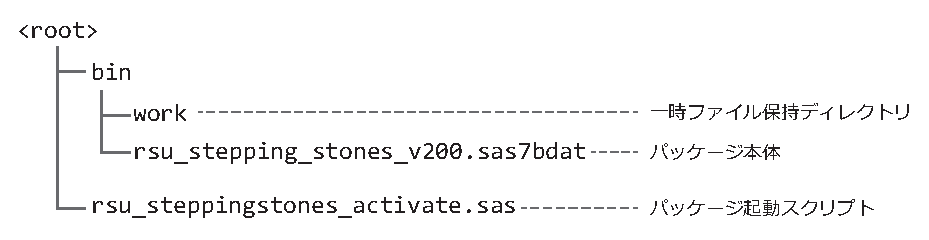
\includegraphics[width=10truecm]{figs/fig_deployment.eps}
\end{center}
\caption{パッケージの配置例}\label{fig:DEPLOYMENT}
\end{figure}
\begin{marker}
モジュール本体を配置するディレクトリ(およびその配下の\texttt{work}ディレクトリ)にはユーザーによる{\bfseries 書き込み権限}が与えられている必要があります。
\end{marker}
\paragraph{推奨設定}
\begin{itemize}
	\item 起動プログラム```\texttt{rsu\_steppingstones\_activate.sas}''配置ディレクトリに``\texttt{bin}''ディレクトリを作成し、そこにモジュール本体を配置します。
	\item SAS起動時実行プログラム``\texttt{appserver\_autoexec\_usermods.sas}''にグローバルマクロ変数 ``\texttt{G\_SAS\_RSU\_DEV\_MODULE\_ROOT\_DIR}''の設定とsasautosオプションの設定をしておきます(\coderef{sasautos})。
\end{itemize}
 
\begin{lstlisting}[language=SAS, caption={\texttt{appserver\_autoexec\_usermods.sas}における設定内容例}, label={code:sasautos}, breaklines = true]
...
%global /readonly G_SAS_RSU_DEV_MODULE_ROOT_DIR = /sas/RSU/RSU_DevModule;
options insert = (sasautos = ("&G_SAS_RSU_DEV_MODULE_ROOT_DIR."));
...
\end{lstlisting}
 
こうすることで、\RDM の起動が容易になります(次節参照)。
 
%%%% Sec.2-2: RSU Development Module 使い方 %%%%
\section{\DocStrTitleRDMHowToUse}
RSU Develoment Moduleの機能を使用するには、{\bfseries セッションごと}にモジュールを起動する必要があります。以下に起動手順を示します。
\begin{enumerate}
\item グローバルマクロ変数 ``\texttt{G\_SAS\_RSU\_DEV\_MODULE\_ROOT\_DIR}''に起動プログラム``\texttt{rsu\_steppingstones\_activate}''を配置したディレクトリの絶対パスを設定します。
\item マクロ``\texttt{rsu\_steppingstones\_activate}''を実行します\footnote{このマクロは\texttt{rsu\_steppingstones\_activate.sas}ファイルに定義されています。}。
\end{enumerate}
\begin{lstlisting}[language=SAS, caption={RSU Stepping Stones 使用例}, label={code:activation}, breaklines = true]
%global G_SAS_RSU_DEV_MODULE_ROOT_DIR;
%let G_SAS_RSU_DEV_MODULE_ROOT_DIR = /sas/RSU/RSU_DevModule;					/* モジュールのパス設定 */
 
%include "&G_SAS_RSU_DEV_MODULE_ROOT_DIR./rsu_dev_module_activate.sas";
%rsu_dev_module_activate(i_dir = /sas/RSU/RSU_DevModule)							/* モジュール起動(モジュール本体を配置したディレクトリを指定) */
 
%&RSUSys.ShowModuleInfo																		/* モジュールの機能実行例 */
\end{lstlisting}
 
前節で示した推奨設定を行ってある場合、自身のプログラムの先頭に\texttt{\%rsu\_steppingstones\_activate}と記述するだけでモジュールの起動が完了します(\coderef{activation_revised})。
\begin{lstlisting}[language=SAS, caption={RSU Steppting Stones起動例}, label={code:activation_revised}, breaklines = true]
%rsu_steppginstones_activate													/* モジュール起動(パスの指定不要) */
 
%&RSUSys.ShowModuleInfo															/* モジュールの機能実行例 */
\end{lstlisting}
\begin{marker}
モジュール配置ディレクトリに複数のバージョンのモジュールが配置してある場合、上記コードによって最新バージョンのものが選択・起動されます。
\end{marker}
 
\paragraph{起動マクロ詳細}
モジュール配置ディレクトリに複数のバージョンのモジュールが配置してある場合、下記コードによって使用バージョンを指定できます。
\begin{lstlisting}[language=SAS, caption={RSU Stepping Stones 起動例(バージョン指定)}, label={code:activation_revised_versioned}, breaklines = true]
%rsu_steppginstones_activate(i_version = 180)							/* モジュール起動(バージョン 1.8.0) */
 
%&RSUSys.ShowModuleInfo															/* モジュールの機能実行例 */
\end{lstlisting}
 
%%%%%%%%%%%%%%%%%%%%%%%%%%%%%%%%%%%%%%%%%%%%%%%%%%%%%
%%%%%%%%%%%%%%%%%%%%%%%%%%%%%%%%%%%%%%%%%%%%%%%%%%%%%
%
% Part.2: リファレンスガイド
%
%%%%%%%%%%%%%%%%%%%%%%%%%%%%%%%%%%%%%%%%%%%%%%%%%%%%%
%%%%%%%%%%%%%%%%%%%%%%%%%%%%%%%%%%%%%%%%%%%%%%%%%%%%%
\part{\DocStrTitleReferenceManual}
 
%%%%%%%%%%%%%%%%%%%%%%%%%%%%%%%%%%%%%%%%%%%%%%%%%%%%%
% Chp.3: 予約済みマクロ変数
%%%%%%%%%%%%%%%%%%%%%%%%%%%%%%%%%%%%%%%%%%%%%%%%%%%%%
\chapter{\DocStrTitleRDMReservedMacVars}
\section{グローバル定数}
以下の変数はモジュール内で使用される読み取り専用グローバル変数です。
\begin{marker}
プログラム内で同名のグローバル変数を宣言したり、当該変数を書き換えようとするとエラーが発生し、処理が中断します。
\end{marker}
 
%%%%%% Table of global constants %%%%%
\begin{center}
{\footnotesize
\begin{xltabular}{\textwidth}{|p{5truecm}|X|p{5truecm}|}
\hline
\thead{\DocStrHeaderGlobalConstantName}&\thead{\DocStrDescription}&\thead{\DocStrHeaderGlobalConstantValue}\\
\hline
\hline
\texttt{RSUArray}&配列パッケージ Prefix&\texttt{RSUArray\_\_}\\
\hline
\texttt{RSUBool}&Boolean構造体&\texttt{RSUBoolean\_\_}\\
\hline
\texttt{RSUClass}&クラスパッケージ Prefix&\texttt{RSUClass\_\_}\\
\hline
\texttt{RSUCounter}&配列パッケージ Prefix&\texttt{RSUCounter\_\_}\\
\hline
\texttt{RSUDS}&データセットパッケージ Prefix&\texttt{RSUDS\_\_}\\
\hline
\texttt{RSUDate}&日付パッケージ Prefix&\texttt{RSUDate\_\_}\\
\hline
\texttt{RSUDayWeek}&曜日構造体&\texttt{RSUDayWeek\_\_}\\
\hline
\texttt{RSUDebug}&デバッグパッケージ Prefix&\texttt{RSUDebug\_\_}\\
\hline
\texttt{RSUDic}&連想配列パッケージ Prefix&\texttt{RSUDic\_\_}\\
\hline
\texttt{RSUDir}&ディレクトリパッケージ Prefix&\texttt{RSUDir\_\_}\\
\hline
\texttt{RSUDirection}&Direction構造体&\texttt{RSUDirection\_\_}\\
\hline
\texttt{RSUExcel}&エクセルファイルパッケージ Prefix&\texttt{RSUExcel\_\_}\\
\hline
\texttt{RSUExecMode}&実行モード構造体&\texttt{RSUExecMode\_\_}\\
\hline
\texttt{RSUExeclDateOffset}&Execlの日付とSASの日付の原点のオフセット&\texttt{21916}\\
\hline
\texttt{RSUFile}&ディレクトリパッケージ Prefix&\texttt{RSUFile\_\_}\\
\hline
\texttt{RSUFileType}&ファイル種別構造体&\texttt{RSUFileType\_\_}\\
\hline
\texttt{RSULf}&複数行表示の際の改行記号&\texttt{|}\\
\hline
\texttt{RSULib}&ライブラリパッケージ Prefix&\texttt{RSULib\_\_}\\
\hline
\texttt{RSUList}&リストパッケージ Prefix&\texttt{RSUList\_\_}\\
\hline
\texttt{RSULogger}&ロガーパッケージ Prefix&\texttt{RSULogger\_\_}\\
\hline
\texttt{RSUMsg}&メッセージパッケージ Prefix&\texttt{RSUMsg\_\_}\\
\hline
\texttt{RSUNUL}&区切り文字Null(00x)&\texttt{'00'x}\\
\hline
\texttt{RSUQueue}&キューパッケージ Prefix&\texttt{RSUQueue\_\_}\\
\hline
\texttt{RSURegex}&正規表現パッケージ Prefix&\texttt{RSURegex\_\_}\\
\hline
\texttt{RSURest}&Rest パッケージ Prefix&\texttt{RSURest\_\_}\\
\hline
\texttt{RSUSkipCol}&読み込みの際、スキップするカラムの指定&\texttt{-}\\
\hline
\texttt{RSUSkippedVar}&ダミー変数名&\texttt{\_\_skipped\_var\_\_}\\
\hline
\texttt{RSUSplitChar}&ファイルパス区切り(LINUX)&\texttt{/}\\
\hline
\texttt{RSUStack}&スタックパッケージ Prefix&\texttt{RSUStack\_\_}\\
\hline
\texttt{RSUStruct}&Structパッケージ Prefix&\texttt{RSUStruct\_\_}\\
\hline
\texttt{RSUSys}&システムパッケージ Prefix&\texttt{RSUSys\_\_}\\
\hline
\texttt{RSUTab}&区切り文字タブ(09x)&\texttt{'09'x}\\
\hline
\texttt{RSUText}&テキストパッケージ Prefix&\texttt{RSUText\_\_}\\
\hline
\texttt{RSUTimer}&タイマーパッケージ Prefix&\texttt{RSUTimer\_\_}\\
\hline
\texttt{RSUUtil}&ユーティリティパッケージ Prefix&\texttt{RSUUtil\_\_}\\
\hline
\texttt{RSU\_G\_ACTIVATED}&RSU Develoment Module 本体名&\texttt{1}\\
\hline
\texttt{RSU\_G\_ARRAY\_DELIMITER}&配列要素の区切り文字&\texttt{`}\\
\hline
\texttt{RSU\_G\_CLASS\_DEFINITION\_DIR}&クラスファイルが作られるディレクトリパス&環境依存(例:\texttt{/sas/RSU/RSU\_DevModule})\\
\hline
\texttt{RSU\_G\_CLASS\_FILE\_COUNTER}&カウンタークラス定義ファイル名&\texttt{RSU\_PKG\_Class\_Counter}\\
\hline
\texttt{RSU\_G\_CLASS\_FILE\_DS\_ITERATOR}&データセットイテレータクラス定義ファイル&\texttt{RSU\_PKG\_Class\_IteratorDS}\\
\hline
\texttt{RSU\_G\_CLASS\_FILE\_FILEWRITER}&ファイルライタークラス定義ファイル名&\texttt{RSU\_PKG\_Class\_FileWriter}\\
\hline
\texttt{RSU\_G\_CLASS\_FILE\_FILE\_ITERATOR}&ファイルイテレータクラス定義ファイル名&\texttt{RSU\_PKG\_Class\_IteratorTextFile}\\
\hline
\texttt{RSU\_G\_CLASS\_FILE\_ITERATOR}&イテレータクラス定義ファイル名&\texttt{RSU\_PKG\_Class\_IteratorArray}\\
\hline
\texttt{RSU\_G\_CLASS\_FILE\_LIB}&ライブラリクラス定義ファイル名&\texttt{RSU\_PKG\_Class\_Lib}\\
\hline
\texttt{RSU\_G\_CLASS\_FILE\_MESSAGE}&メッセージ出力クラス定義ファイル名&\texttt{RSU\_PKG\_Class\_Message}\\
\hline
\texttt{RSU\_G\_CLASS\_FILE\_PROGRESS\_BAR}&プログレスバークラス定義ファイル&\texttt{RSU\_PKG\_Class\_ProgressBar}\\
\hline
\texttt{RSU\_G\_CLASS\_FILE\_REGEX\_ITE}&正規表現クラス定義ファイル名&\texttt{RSU\_PKG\_Class\_IteratorRegex}\\
\hline
\texttt{RSU\_G\_CLASS\_FILE\_REST}&Rest クラス定義ファイル名&\texttt{RSU\_PKG\_Class\_Rest}\\
\hline
\texttt{RSU\_G\_CLASS\_FILE\_TIMER}&タイマークラス定義ファイル名&\texttt{RSU\_PKG\_Class\_Timer}\\
\hline
\texttt{RSU\_G\_DATASET\_ID\_DIGIT}&データベース名のID部の桁数&\texttt{6}\\
\hline
\texttt{RSU\_G\_DEV\_MODULE\_NAME}&選択された RSU Develoment Module 本体名&環境依存(例:\texttt{rsu\_dev\_module\_v200})\\
\hline
\texttt{RSU\_G\_DEV\_MODULE\_NAME\_BODY}&RSU Development Moduleの本体名&\texttt{RSU\_DEV\_MODULE}\\
\hline
\texttt{RSU\_G\_INSTANCE\_ID\_DIGIT}&インスタンス名のID部の桁数&\texttt{4}\\
\hline
\texttt{RSU\_G\_INSTANCE\_PREFIX}&インスタンス名に付与されるprefix&\texttt{RI\_}\\
\hline
\texttt{RSU\_G\_KEY\_PREFIX}&連想配列の検索キーのPrefix&\texttt{\#KEY:}\\
\hline
\texttt{RSU\_G\_MACRO\_DEF\_TMP\_FILE}&クラス定義用一時ファイル名&\texttt{rsu\_class\_instantiate}\\
\hline
\texttt{RSU\_G\_MSG\_INDENT\_ERROR}&Error 表示時のインデント&\texttt{ERROR-␣␣␣␣}\\
\hline
\texttt{RSU\_G\_MSG\_INDENT\_NOTE}&Note 表示時のインデント&\texttt{␣␣␣␣␣␣␣␣}\\
\hline
\texttt{RSU\_G\_MSG\_INDENT\_PLANE}&平文表示時のインデント&\texttt{␣␣␣␣␣␣␣␣}\\
\hline
\texttt{RSU\_G\_MSG\_INDENT\_WARNING}&Warning 表示時のインデント&\texttt{WARNING-}\\
\hline
\texttt{RSU\_G\_PATH\_SPLITTER}&パスのセパレータ&\texttt{/}\\
\hline
\texttt{\_\_debug}&デバッグコードの終端文字列&\texttt{/}\\
\hline
\texttt{\_\_release}&リリースコードの終端文字列&\texttt{/}\\
\hline
\end{xltabular}
}
\end{center}
 
\section{グローバルマクロ変数}
以下の変数はモジュール内で使用されるグローバル変数です。
\begin{marker}
これらグローバル変数の値は書き換え可能ですが(モジュール側で書き換え制限を課せられないため)、絶対にプログラム中に削除したり、書き換えたりしないでください。予測不能な結果をもたらす可能性があります。
\end{marker}
 
%%%%% Table of global variables %%%%%
\begin{center}
{\footnotesize
\begin{xltabular}{\textwidth}{|p{5truecm}|X|}
\hline
\thead{\DocStrHeaderGlobalVariableName}&\thead{\DocStrDescription}\\
\hline
\hline
\texttt{RSU\_g\_dic\_write\_protected}&データセット書き込み禁止設定用(Dictionary)\\
\hline
\texttt{RSU\_g\_log\_conf\_log\_level}&現在のログ表示レベル\\
\hline
\texttt{RSU\_g\_log\_conf\_show\_arguments}&マクロ呼び出しトレースにおいて引数を表示するか\\
\hline
\texttt{RSU\_g\_log\_conf\_show\_macro}&マクロ呼び出しトレースを表示するか\\
\hline
\texttt{RSU\_g\_sequence\_dataset}&データセット名用連番\\
\hline
\texttt{RSU\_g\_sequence\_directory}&ディレクトリ名用連番\\
\hline
\texttt{RSU\_g\_sequence\_ds\_snapshot}&データセットスナップショット用連番\\
\hline
\texttt{RSU\_g\_sequence\_footpint}&デバッグ用フットプリント用連番\\
\hline
\texttt{RSU\_g\_sequence\_instance}&クラスインスタンス名用連番\\
\hline
\texttt{RSU\_g\_sequence\_library}&ライブラリ名用連番\\
\hline
\texttt{RSU\_g\_sequence\_macro\_snapshot}&マクロスナップショット用連番\\
\hline
\end{xltabular}
}
\end{center}
 
%%%%%%%%%%%%%%%%%%%%%%%%%%%%%%%%%%%%%%%%%%%%%%%%%%%%%
% Chp.4: 事前定義フォーマット
%%%%%%%%%%%%%%%%%%%%%%%%%%%%%%%%%%%%%%%%%%%%%%%%%%%%%
\chapter{\DocStrTitleRDMPredefinedFormat}
 
\section{\texttt{RSU\_fmt\_boolean\_en}}
\paragraph{\DocStrTitleRDMPredefinedFormatConversion}Boolean数値 \ding{224} Boolean 英語
%%%%% Table of format components %%%%%
\begin{center}
\begin{xltabular}{\textwidth}{|p{7truecm}|X|}
\hline
\thead{\DocStrHeaderFormatInput}&\thead{\DocStrHeaderFormatOutput}\\
\hline
\hline
\texttt{0}&\texttt{"True"}\\
\hline
\texttt{1}&\texttt{"False"}\\
\hline
\end{xltabular}
\end{center}
\section{\texttt{RSU\_fmt\_boolean\_jp}}
\paragraph{\DocStrTitleRDMPredefinedFormatConversion}Boolean数値 \ding{224} Boolean 日本語
%%%%% Table of format components %%%%%
\begin{center}
\begin{xltabular}{\textwidth}{|p{7truecm}|X|}
\hline
\thead{\DocStrHeaderFormatInput}&\thead{\DocStrHeaderFormatOutput}\\
\hline
\hline
\texttt{0}&\texttt{"真"}\\
\hline
\texttt{1}&\texttt{"偽"}\\
\hline
\end{xltabular}
\end{center}
\section{\texttt{\$RSU\_fmt\_inv\_weekday\_en\_long}}
\paragraph{\DocStrTitleRDMPredefinedFormatConversion}曜日英語 \ding{224} 曜日数値
%%%%% Table of format components %%%%%
\begin{center}
\begin{xltabular}{\textwidth}{|p{7truecm}|X|}
\hline
\thead{\DocStrHeaderFormatInput}&\thead{\DocStrHeaderFormatOutput}\\
\hline
\hline
\texttt{"SUNDAY"}&\texttt{"1"}\\
\hline
\texttt{"MONDAY"}&\texttt{"2"}\\
\hline
\texttt{"TUESDAY"}&\texttt{"3"}\\
\hline
\texttt{"WEDNESDAY"}&\texttt{"4"}\\
\hline
\texttt{"THURSDAY"}&\texttt{"5"}\\
\hline
\texttt{"FRIDAY"}&\texttt{"6"}\\
\hline
\texttt{"SATURDAY"}&\texttt{"7"}\\
\hline
\end{xltabular}
\end{center}
\section{\texttt{\$RSU\_fmt\_inv\_weekday\_en\_short}}
\paragraph{\DocStrTitleRDMPredefinedFormatConversion}曜日英語略称 \ding{224} 曜日数値
%%%%% Table of format components %%%%%
\begin{center}
\begin{xltabular}{\textwidth}{|p{7truecm}|X|}
\hline
\thead{\DocStrHeaderFormatInput}&\thead{\DocStrHeaderFormatOutput}\\
\hline
\hline
\texttt{"SUN"}&\texttt{"1"}\\
\hline
\texttt{"MON"}&\texttt{"2"}\\
\hline
\texttt{"TUE"}&\texttt{"3"}\\
\hline
\texttt{"WED"}&\texttt{"4"}\\
\hline
\texttt{"THU"}&\texttt{"5"}\\
\hline
\texttt{"FRI"}&\texttt{"6"}\\
\hline
\texttt{"SAT"}&\texttt{"7"}\\
\hline
\end{xltabular}
\end{center}
\section{\texttt{\$RSU\_fmt\_inv\_weekday\_jp\_long}}
\paragraph{\DocStrTitleRDMPredefinedFormatConversion}曜日日本語 \ding{224} 曜日数値
%%%%% Table of format components %%%%%
\begin{center}
\begin{xltabular}{\textwidth}{|p{7truecm}|X|}
\hline
\thead{\DocStrHeaderFormatInput}&\thead{\DocStrHeaderFormatOutput}\\
\hline
\hline
\texttt{"日曜日"}&\texttt{"1"}\\
\hline
\texttt{"月曜日"}&\texttt{"2"}\\
\hline
\texttt{"火曜日"}&\texttt{"3"}\\
\hline
\texttt{"水曜日"}&\texttt{"4"}\\
\hline
\texttt{"木曜日"}&\texttt{"5"}\\
\hline
\texttt{"金曜日"}&\texttt{"6"}\\
\hline
\texttt{"土曜日"}&\texttt{"7"}\\
\hline
\end{xltabular}
\end{center}
\section{\texttt{\$RSU\_fmt\_inv\_weekday\_jp\_short}}
\paragraph{\DocStrTitleRDMPredefinedFormatConversion}曜日日本語略称 \ding{224} 曜日数値
%%%%% Table of format components %%%%%
\begin{center}
\begin{xltabular}{\textwidth}{|p{7truecm}|X|}
\hline
\thead{\DocStrHeaderFormatInput}&\thead{\DocStrHeaderFormatOutput}\\
\hline
\hline
\texttt{"日"}&\texttt{"1"}\\
\hline
\texttt{"月"}&\texttt{"2"}\\
\hline
\texttt{"火"}&\texttt{"3"}\\
\hline
\texttt{"水"}&\texttt{"4"}\\
\hline
\texttt{"木"}&\texttt{"5"}\\
\hline
\texttt{"金"}&\texttt{"6"}\\
\hline
\texttt{"土"}&\texttt{"7"}\\
\hline
\end{xltabular}
\end{center}
\section{\texttt{RSU\_fmt\_month\_name\_en}}
\paragraph{\DocStrTitleRDMPredefinedFormatConversion}月番号 \ding{224} 英語月名
%%%%% Table of format components %%%%%
\begin{center}
\begin{xltabular}{\textwidth}{|p{7truecm}|X|}
\hline
\thead{\DocStrHeaderFormatInput}&\thead{\DocStrHeaderFormatOutput}\\
\hline
\hline
\texttt{1}&\texttt{"Junuary"}\\
\hline
\texttt{2}&\texttt{"February"}\\
\hline
\texttt{3}&\texttt{"March"}\\
\hline
\texttt{4}&\texttt{"April"}\\
\hline
\texttt{5}&\texttt{"May"}\\
\hline
\texttt{6}&\texttt{"June"}\\
\hline
\texttt{7}&\texttt{"July"}\\
\hline
\texttt{8}&\texttt{"August"}\\
\hline
\texttt{9}&\texttt{"September"}\\
\hline
\texttt{10}&\texttt{"October"}\\
\hline
\texttt{11}&\texttt{"November"}\\
\hline
\texttt{12}&\texttt{"December"}\\
\hline
\end{xltabular}
\end{center}
\section{\texttt{RSU\_fmt\_month\_name\_en\_short}}
\paragraph{\DocStrTitleRDMPredefinedFormatConversion}月番号 \ding{224} 英語月名(略)
%%%%% Table of format components %%%%%
\begin{center}
\begin{xltabular}{\textwidth}{|p{7truecm}|X|}
\hline
\thead{\DocStrHeaderFormatInput}&\thead{\DocStrHeaderFormatOutput}\\
\hline
\hline
\texttt{1}&\texttt{"Jun"}\\
\hline
\texttt{2}&\texttt{"Feb"}\\
\hline
\texttt{3}&\texttt{"Mar"}\\
\hline
\texttt{4}&\texttt{"Apr"}\\
\hline
\texttt{5}&\texttt{"May"}\\
\hline
\texttt{6}&\texttt{"Jun"}\\
\hline
\texttt{7}&\texttt{"Jul"}\\
\hline
\texttt{8}&\texttt{"Aug"}\\
\hline
\texttt{9}&\texttt{"Sep"}\\
\hline
\texttt{10}&\texttt{"Oct"}\\
\hline
\texttt{11}&\texttt{"Nov"}\\
\hline
\texttt{12}&\texttt{"Dec"}\\
\hline
\end{xltabular}
\end{center}
\section{\texttt{RSU\_fmt\_month\_name\_jp}}
\paragraph{\DocStrTitleRDMPredefinedFormatConversion}月番号 \ding{224} 日本語月名
%%%%% Table of format components %%%%%
\begin{center}
\begin{xltabular}{\textwidth}{|p{7truecm}|X|}
\hline
\thead{\DocStrHeaderFormatInput}&\thead{\DocStrHeaderFormatOutput}\\
\hline
\hline
\texttt{1}&\texttt{"1月"}\\
\hline
\texttt{2}&\texttt{"2月"}\\
\hline
\texttt{3}&\texttt{"3月"}\\
\hline
\texttt{4}&\texttt{"4月"}\\
\hline
\texttt{5}&\texttt{"5月"}\\
\hline
\texttt{6}&\texttt{"6月"}\\
\hline
\texttt{7}&\texttt{"7月"}\\
\hline
\texttt{8}&\texttt{"8月"}\\
\hline
\texttt{9}&\texttt{"9月"}\\
\hline
\texttt{10}&\texttt{"10月"}\\
\hline
\texttt{11}&\texttt{"11月"}\\
\hline
\texttt{12}&\texttt{"12月"}\\
\hline
\end{xltabular}
\end{center}
\section{\texttt{RSU\_fmt\_weekday\_en\_long}}
\paragraph{\DocStrTitleRDMPredefinedFormatConversion}曜日数値 \ding{224} 曜日英語
%%%%% Table of format components %%%%%
\begin{center}
\begin{xltabular}{\textwidth}{|p{7truecm}|X|}
\hline
\thead{\DocStrHeaderFormatInput}&\thead{\DocStrHeaderFormatOutput}\\
\hline
\hline
\texttt{1}&\texttt{"Sunday"}\\
\hline
\texttt{2}&\texttt{"Monday"}\\
\hline
\texttt{3}&\texttt{"Tuesday"}\\
\hline
\texttt{4}&\texttt{"Wednesday"}\\
\hline
\texttt{5}&\texttt{"Thursday"}\\
\hline
\texttt{6}&\texttt{"Friday"}\\
\hline
\texttt{7}&\texttt{"Saturday"}\\
\hline
\end{xltabular}
\end{center}
\section{\texttt{RSU\_fmt\_weekday\_en\_short}}
\paragraph{\DocStrTitleRDMPredefinedFormatConversion}曜日数値 \ding{224} 曜日英語略称
%%%%% Table of format components %%%%%
\begin{center}
\begin{xltabular}{\textwidth}{|p{7truecm}|X|}
\hline
\thead{\DocStrHeaderFormatInput}&\thead{\DocStrHeaderFormatOutput}\\
\hline
\hline
\texttt{1}&\texttt{"Sun"}\\
\hline
\texttt{2}&\texttt{"Mon"}\\
\hline
\texttt{3}&\texttt{"Tues"}\\
\hline
\texttt{4}&\texttt{"Wed"}\\
\hline
\texttt{5}&\texttt{"Thu"}\\
\hline
\texttt{6}&\texttt{"Fri"}\\
\hline
\texttt{7}&\texttt{"Sat"}\\
\hline
\end{xltabular}
\end{center}
\section{\texttt{RSU\_fmt\_weekday\_jp\_long}}
\paragraph{\DocStrTitleRDMPredefinedFormatConversion}曜日数値 \ding{224} 曜日日本語
%%%%% Table of format components %%%%%
\begin{center}
\begin{xltabular}{\textwidth}{|p{7truecm}|X|}
\hline
\thead{\DocStrHeaderFormatInput}&\thead{\DocStrHeaderFormatOutput}\\
\hline
\hline
\texttt{1}&\texttt{"日曜日"}\\
\hline
\texttt{2}&\texttt{"月曜日"}\\
\hline
\texttt{3}&\texttt{"火曜日"}\\
\hline
\texttt{4}&\texttt{"水曜日"}\\
\hline
\texttt{5}&\texttt{"木曜日"}\\
\hline
\texttt{6}&\texttt{"金曜日"}\\
\hline
\texttt{7}&\texttt{"土曜日"}\\
\hline
\end{xltabular}
\end{center}
\section{\texttt{RSU\_fmt\_weekday\_jp\_short}}
\paragraph{\DocStrTitleRDMPredefinedFormatConversion}曜日数値 \ding{224} 曜日日本語略称
%%%%% Table of format components %%%%%
\begin{center}
\begin{xltabular}{\textwidth}{|p{7truecm}|X|}
\hline
\thead{\DocStrHeaderFormatInput}&\thead{\DocStrHeaderFormatOutput}\\
\hline
\hline
\texttt{1}&\texttt{"日"}\\
\hline
\texttt{2}&\texttt{"月"}\\
\hline
\texttt{3}&\texttt{"火"}\\
\hline
\texttt{4}&\texttt{"水"}\\
\hline
\texttt{5}&\texttt{"木"}\\
\hline
\texttt{6}&\texttt{"金"}\\
\hline
\texttt{7}&\texttt{"土"}\\
\hline
\end{xltabular}
\end{center}
 
%%%%%%%%%%%%%%%%%%%%%%%%%%%%%%%%%%%%%%%%%%%%%%%%%%%%%
% Chp.5: 事前定義構造体
%%%%%%%%%%%%%%%%%%%%%%%%%%%%%%%%%%%%%%%%%%%%%%%%%%%%%
\chapter{\DocStrTitleRDMPredefStructure}
\RDM は``構造体''のごとき機能を提供します。
構造体のメンバーへのアクセスは、``\texttt{\%\&}<構造体名>\texttt{.}<メンバー名>''とします。
 
例えば、構造体``\texttt{RSUBool}''は``\texttt{True}''と``\texttt{False}''の2つのメンバーを持ち、\coderef{structure_example}のような記法でメンバー値を取得出来ます。
\begin{lstlisting}[language=SAS, caption={構造体の使用例}, label={code:structure_example}, breaklines = true]
%macro Structure_Sample(i_boolean =);
	%if (&i_boolean.) %then %do;
		%put 真;
	%end;
	%else %do;
		%put 偽;
	%end;
%mend Structure_Sample;
 
%Structure_Sample(i_boolean = %&RSUBool.True)		/* 構造体 RSUBool のメンバーへのアクセス */
\end{lstlisting}
\section{\texttt{RSUBool}}
\paragraph{\DocStrDescription}Boolean構造体
%%%%% Table of structure members %%%%%
\begin{center}
{\footnotesize
\begin{xltabular}{\textwidth}{|p{5truecm}|p{2truecm}|X|}
\hline
\thead{\DocStrHeaderStructMemberName}&\thead{\DocStrHeaderStructMemberValue}&\thead{\DocStrDescription}\\
\hline
\hline
\texttt{True}&\texttt{	1}&Boolean 真値\\
\hline
\texttt{False}&\texttt{	0}&Boolean 偽値\\
\hline
\end{xltabular}
}
\end{center}
\section{\texttt{RSUDayWeek}}
\paragraph{\DocStrDescription}曜日構造体
%%%%% Table of structure members %%%%%
\begin{center}
{\footnotesize
\begin{xltabular}{\textwidth}{|p{5truecm}|p{2truecm}|X|}
\hline
\thead{\DocStrHeaderStructMemberName}&\thead{\DocStrHeaderStructMemberValue}&\thead{\DocStrDescription}\\
\hline
\hline
\texttt{Sun}&\texttt{	1}&日曜日\\
\hline
\texttt{Mon}&\texttt{	2}&月曜日\\
\hline
\texttt{Tue}&\texttt{	3}&火曜日\\
\hline
\texttt{Wed}&\texttt{	4}&水曜日\\
\hline
\texttt{Thu}&\texttt{	5}&木曜日\\
\hline
\texttt{Fri}&\texttt{	6}&金曜日\\
\hline
\texttt{Sat}&\texttt{	7}&土曜日\\
\hline
\end{xltabular}
}
\end{center}
\section{\texttt{RSUDirection}}
\paragraph{\DocStrDescription}Direction構造体
%%%%% Table of structure members %%%%%
\begin{center}
{\footnotesize
\begin{xltabular}{\textwidth}{|p{5truecm}|p{2truecm}|X|}
\hline
\thead{\DocStrHeaderStructMemberName}&\thead{\DocStrHeaderStructMemberValue}&\thead{\DocStrDescription}\\
\hline
\hline
\texttt{Forward}&\texttt{	1}&イテレータの向き: 前進\\
\hline
\texttt{Backward}&\texttt{	-1}&イテレータの向き: 後進\\
\hline
\end{xltabular}
}
\end{center}
\section{\texttt{RSUExecMode}}
\paragraph{\DocStrDescription}実行モード構造体
%%%%% Table of structure members %%%%%
\begin{center}
{\footnotesize
\begin{xltabular}{\textwidth}{|p{5truecm}|p{2truecm}|X|}
\hline
\thead{\DocStrHeaderStructMemberName}&\thead{\DocStrHeaderStructMemberValue}&\thead{\DocStrDescription}\\
\hline
\hline
\texttt{Debug}&\texttt{	DEBUG}&実行モード: デバッグモード\\
\hline
\texttt{Release}&\texttt{	RELEASE}&実行モード: リリースモード\\
\hline
\end{xltabular}
}
\end{center}
\section{\texttt{RSUFileType}}
\paragraph{\DocStrDescription}ファイル種別構造体
%%%%% Table of structure members %%%%%
\begin{center}
{\footnotesize
\begin{xltabular}{\textwidth}{|p{5truecm}|p{2truecm}|X|}
\hline
\thead{\DocStrHeaderStructMemberName}&\thead{\DocStrHeaderStructMemberValue}&\thead{\DocStrDescription}\\
\hline
\hline
\texttt{File}&\texttt{	F}&ファイル種別: ファイル\\
\hline
\texttt{Directory}&\texttt{	D}&ファイル種別: ディレクトリ\\
\hline
\texttt{Both}&\texttt{	B}&ファイル種別: すべて(ファイル、ディレクトリ)\\
\hline
\end{xltabular}
}
\end{center}
 
%%%%%%%%%%%%%%%%%%%%%%%%%%%%%%%%%%%%%%%%%%%%%%%%%%%%%
% Chp.6+: パッケージ(カテゴリー別に表示)
%%%%%%%%%%%%%%%%%%%%%%%%%%%%%%%%%%%%%%%%%%%%%%%%%%%%%
\chapter{データセットの取り扱いに役立つパッケージ}\label{sec:Cate_DataHandling}
\section{\DocStrTitlePackageListInCategory}
%%%%%%%%%%%%%%%%%%%%%%%%%%%%
% Table of packages in category
%%%%%%%%%%%%%%%%%%%%%%%%%%%%
\begin{center}
\begin{xltabular}{\textwidth}{|p{2truecm}|X|p{2truecm}|}
\hline
\thead{\DocStrHeaderPackageName}&\thead{\DocStrHeaderPackagePurpose}&\thead{\DocStrRefto}\\
\hline
\hline
\texttt{RSUDS}&データセット操作&\secref{RSUDS}\\
\hline
\texttt{RSULib}&ライブラリ操作&\secref{RSULib}\\
\hline
\end{xltabular}
\end{center}
\section{\texttt{RSUDS}\;---\;データセット操作\;---}\label{sec:RSUDS}
SAS データセットに関連する操作を行うマクロ群を提供するパッケージ
%%%%%% Function list %%%%%
\paragraph{\DocStrTitleRDMPackageFunctionList}
\begin{center}
{\footnotesize
\begin{xltabular}{\textwidth}{|p{4truecm}|X|p{1.2truecm}|}
\hline
\thead{\DocStrHeaderFunctionName}&\thead{\DocStrDescription}&\thead{\DocStrRefto}\\
\hline
\hline
\texttt{\%\&RSUDS.Append}&データセットを連結(Append)します&\subsecref{RSUDS_RSUDS__Append}\\
\hline
\texttt{\%\&RSUDS.ArrangeVarOrder}&データセットの変数を並べ替えます&\subsecref{RSUDS_RSUDS__ArrangeVarOrder}\\
\hline
\texttt{\%\&RSUDS.Clone}&データセットを複製します&\subsecref{RSUDS_RSUDS__Clone}\\
\hline
\texttt{\%\&RSUDS.Concat}&データセットを縦結合します&\subsecref{RSUDS_RSUDS__Concat}\\
\hline
\texttt{\%\&RSUDS.CrossJoin}&2つのデータセットの直積を生成します&\subsecref{RSUDS_RSUDS__CrossJoin}\\
\hline
\texttt{\%\&RSUDS.Delete}&データセットを削除します&\subsecref{RSUDS_RSUDS__Delete}\\
\hline
\texttt{\%\&RSUDS.Exists}&データセットが存在しているか否かを返します&\subsecref{RSUDS_RSUDS__Exists}\\
\hline
\texttt{\%\&RSUDS.Fetch}&データセットからレコードをフェッチします。&\subsecref{RSUDS_RSUDS__Fetch}\\
\hline
\texttt{\%\&RSUDS.ForEach}&データセットのレコードの走査&\subsecref{RSUDS_RSUDS__ForEach}\\
\hline
\texttt{\%\&RSUDS.FullJoin}&データセットの Full Join を行います&\subsecref{RSUDS_RSUDS__FullJoin}\\
\hline
\texttt{\%\&RSUDS.Get1stRecord}&データセットの最初のレコードを取得します&\subsecref{RSUDS_RSUDS__Get1stRecord}\\
\hline
\texttt{\%\&RSUDS.GetCount}&指定データセットのレコード数を返します。&\subsecref{RSUDS_RSUDS__GetCount}\\
\hline
\texttt{\%\&RSUDS.GetCurrent}&開いているデータセットの現在のポインタのレコードの値を返します。&\subsecref{RSUDS_RSUDS__GetCurrent}\\
\hline
\texttt{\%\&RSUDS.GetDSDefinition}&データセットの定義を取得します。&\subsecref{RSUDS_RSUDS__GetDSDefinition}\\
\hline
\texttt{\%\&RSUDS.GetDSname}&データセット(1レベル、または2レベル)のデータセット名を返します&\subsecref{RSUDS_RSUDS__GetDSname}\\
\hline
\texttt{\%\&RSUDS.GetIterator}&データセットイテレータを生成します&\subsecref{RSUDS_RSUDS__GetIterator}\\
\hline
\texttt{\%\&RSUDS.GetLabel}&データセットに付与されているラベルを返します&\subsecref{RSUDS_RSUDS__GetLabel}\\
\hline
\texttt{\%\&RSUDS.GetLibname}&データセット(1レベル、または2レベル)のライブラリ名を返します&\subsecref{RSUDS_RSUDS__GetLibname}\\
\hline
\texttt{\%\&RSUDS.GetNoOfVariables}&データセットの変数数を返します&\subsecref{RSUDS_RSUDS__GetNoOfVariables}\\
\hline
\texttt{\%\&RSUDS.GetTempDSName}&一時データセットの名称を返します&\subsecref{RSUDS_RSUDS__GetTempDSName}\\
\hline
\texttt{\%\&RSUDS.GetUniqueList}&指定変数で一意化したデータセットを取得します&\subsecref{RSUDS_RSUDS__GetUniqueList}\\
\hline
\texttt{\%\&RSUDS.GetValue}&指定変数の値を返します&\subsecref{RSUDS_RSUDS__GetValue}\\
\hline
\texttt{\%\&RSUDS.GetVariables}&データセットの変数の配列を返します&\subsecref{RSUDS_RSUDS__GetVariables}\\
\hline
\texttt{\%\&RSUDS.InnerJoin}&データセットの Inner Join を行います&\subsecref{RSUDS_RSUDS__InnerJoin}\\
\hline
\texttt{\%\&RSUDS.IsDSEmpty}&指定データセットが空か否かを返します&\subsecref{RSUDS_RSUDS__IsDSEmpty}\\
\hline
\texttt{\%\&RSUDS.IsVarDefined}&元データセットに指定変数が定義されているか否かを返します&\subsecref{RSUDS_RSUDS__IsVarDefined}\\
\hline
\texttt{\%\&RSUDS.LeftJoin}&データセットの Left Join を行います&\subsecref{RSUDS_RSUDS__LeftJoin}\\
\hline
\texttt{\%\&RSUDS.LoadExcel}&エクセルファイルをインポートします&\subsecref{RSUDS_RSUDS__LoadExcel}\\
\hline
\texttt{\%\&RSUDS.LoadText}&テキストファイルをデータセットにロードします(定義ファイルによってデータセットの定義を行います)&\subsecref{RSUDS_RSUDS__LoadText}\\
\hline
\texttt{\%\&RSUDS.LoadTextIntoFrame}&テキストファイルをデータセットにロードします(既存データセットによってデータセットの定義を行います)&\subsecref{RSUDS_RSUDS__LoadTextIntoFrame}\\
\hline
\texttt{\%\&RSUDS.Lock}&データセットの排他ロックを取得します(取得するまで待機)&\subsecref{RSUDS_RSUDS__Lock}\\
\hline
\texttt{\%\&RSUDS.Print}&データセットの内容をログに出力します&\subsecref{RSUDS_RSUDS__Print}\\
\hline
\texttt{\%\&RSUDS.Protect}&データセットを書き込み禁止にします&\subsecref{RSUDS_RSUDS__Protect}\\
\hline
\texttt{\%\&RSUDS.ReplaceNullC}&データセットの欠損値を指定値で置き換えます(文字型のみ)&\subsecref{RSUDS_RSUDS__ReplaceNullC}\\
\hline
\texttt{\%\&RSUDS.ReplaceNullN}&データセットの欠損値を指定値で置き換えます(数値型のみ)&\subsecref{RSUDS_RSUDS__ReplaceNullN}\\
\hline
\texttt{\%\&RSUDS.SaveAs}&データセットを指定ディレクトリに保存します&\subsecref{RSUDS_RSUDS__SaveAs}\\
\hline
\texttt{\%\&RSUDS.SaveAsExcel}&データセットをExcelで保存します&\subsecref{RSUDS_RSUDS__SaveAsExcel}\\
\hline
\texttt{\%\&RSUDS.SaveAsText}&データセットをテキストで保存します&\subsecref{RSUDS_RSUDS__SaveAsText}\\
\hline
\texttt{\%\&RSUDS.Subtract}&左側データセットから右側データセットとの共通部分を取り除きます&\subsecref{RSUDS_RSUDS__Subtract}\\
\hline
\texttt{\%\&RSUDS.TerminateLoop}&ループを強制終了します&\subsecref{RSUDS_RSUDS__TerminateLoop}\\
\hline
\texttt{\%\&RSUDS.Unlock}&データセットの排他ロックを開放します&\subsecref{RSUDS_RSUDS__Unlock}\\
\hline
\texttt{\%\&RSUDS.Unprotect}&データセットの書き込み禁止を解除します&\subsecref{RSUDS_RSUDS__Unprotect}\\
\hline
\texttt{\%\&RSUDS.Update}&データセットUpdateを実行します&\subsecref{RSUDS_RSUDS__Update}\\
\hline
\texttt{\%\&RSUDS.VerifyExists}&データセットの存在を検証します(検証に失敗した場合処理が中断します)&\subsecref{RSUDS_RSUDS__VerifyExists}\\
\hline
\end{xltabular}
}
\end{center}
\subsection{\texttt{Append}}\label{subsec:RSUDS_RSUDS__Append}
データセットを連結(Append)します
%%%%% Function Detail %%%%%
\paragraph{\DocStrDetails}
Append元が存在しない場合は新規に生成します
{\small
\begin{DefFunc}{\texttt{\%\&RSUDS.Append}}
\begin{tabular}{rl}
\makecell[r]{\bfseries \DocStrTitleFunctionDefinition :}&\begin{minipage}[t]{\RSUFuncArgWidth}
%%%%%%%%%%%%%%%%%%%%%%%%%%%%%%%%%%%%%%%%%
%  Definition
%%%%%%%%%%%%%%%%%%%%%%%%%%%%%%%%%%%%%%%%%
\begin{verbatim}
%macro RSUDS__Append(
							iods_base_ds =
							, ids_data_ds =
							);
\end{verbatim}
\end{minipage}\\\\
%%%%%%%%%%%%%%%%%%%%%%%%%%%%%%%%%%%%%%%%%
%  Return value
%%%%%%%%%%%%%%%%%%%%%%%%%%%%%%%%%%%%%%%%%
\makecell[r]{\bfseries \DocStrTitleFunctionReturn :}&\DocStrFunctionNoReturn\\\\
%%%%%%%%%%%%%%%%%%%%%%%%%%%%%%%%%%%%%%%%%
%  Argument table
%%%%%%%%%%%%%%%%%%%%%%%%%%%%%%%%%%%%%%%%%
\makecell[r]{\bfseries \DocStrTitleFunctionArgument :}&\begin{minipage}[t]{\RSUFuncArgWidth}\vspace*{-7pt}
\begin{tabularx}{\RSUFuncArgWidth}{|l|X|c|}
\hline
\thead{\DocStrHeaderFunctionArgumentVariable}&\thead{\DocStrDescription}&\thead{\DocStrHeaderFunctionArgumentRequired}\\
\hline
\hline
\texttt{iods\_base\_ds}&Append元データセット&\ding{51}\\
\hline
\texttt{ids\_data\_ds}&Appendするデータセット&\ding{51}\\
\hline
\end{tabularx}
\end{minipage}\\\\
\end{tabular}
%%%%% Funcion Note %%%%%
\vskip\baselineskip
\begin{marker}
内部では\texttt{proc append}を呼び出しているので、元データセットと追加データセットの定義が異なるなどの不整合がある場合にはエラーになります
\end{marker}
\end{DefFunc}
}
\subsection{\texttt{ArrangeVarOrder}}\label{subsec:RSUDS_RSUDS__ArrangeVarOrder}
データセットの変数を並べ替えます
{\small
\begin{DefFunc}{\texttt{\%\&RSUDS.ArrangeVarOrder}}
\begin{tabular}{rl}
\makecell[r]{\bfseries \DocStrTitleFunctionDefinition :}&\begin{minipage}[t]{\RSUFuncArgWidth}
%%%%%%%%%%%%%%%%%%%%%%%%%%%%%%%%%%%%%%%%%
%  Definition
%%%%%%%%%%%%%%%%%%%%%%%%%%%%%%%%%%%%%%%%%
\begin{verbatim}
%macro RSUDS__ArrangeVarOrder(
										iods_dataset =
										, i_leading_vars =
										, i_following_vars =
										);
\end{verbatim}
\end{minipage}\\\\
%%%%%%%%%%%%%%%%%%%%%%%%%%%%%%%%%%%%%%%%%
%  Return value
%%%%%%%%%%%%%%%%%%%%%%%%%%%%%%%%%%%%%%%%%
\makecell[r]{\bfseries \DocStrTitleFunctionReturn :}&\DocStrFunctionNoReturn\\\\
%%%%%%%%%%%%%%%%%%%%%%%%%%%%%%%%%%%%%%%%%
%  Argument table
%%%%%%%%%%%%%%%%%%%%%%%%%%%%%%%%%%%%%%%%%
\makecell[r]{\bfseries \DocStrTitleFunctionArgument :}&\begin{minipage}[t]{\RSUFuncArgWidth}\vspace*{-7pt}
\begin{tabularx}{\RSUFuncArgWidth}{|l|X|c|}
\hline
\thead{\DocStrHeaderFunctionArgumentVariable}&\thead{\DocStrDescription}&\thead{\DocStrHeaderFunctionArgumentRequired}\\
\hline
\hline
\texttt{iods\_dataset}&入力データセット&\ding{51}\\
\hline
\texttt{i\_leading\_vars}&先行させる変数リスト&\\
\hline
\texttt{i\_following\_vars}&後方に移動させる変数リスト&\\
\hline
\end{tabularx}
\end{minipage}\\\\
\end{tabular}
\end{DefFunc}
}
\subsection{\texttt{Clone}}\label{subsec:RSUDS_RSUDS__Clone}
データセットを複製します
{\small
\begin{DefFunc}{\texttt{\%\&RSUDS.Clone}}
\begin{tabular}{rl}
\makecell[r]{\bfseries \DocStrTitleFunctionDefinition :}&\begin{minipage}[t]{\RSUFuncArgWidth}
%%%%%%%%%%%%%%%%%%%%%%%%%%%%%%%%%%%%%%%%%
%  Definition
%%%%%%%%%%%%%%%%%%%%%%%%%%%%%%%%%%%%%%%%%
\begin{verbatim}
%macro RSUDS__Clone(
						ids_dataset =
						, ods_cloned_dataset =
						, i_modifier =
						, i_mod_pos = POST
						);
\end{verbatim}
\end{minipage}\\\\
%%%%%%%%%%%%%%%%%%%%%%%%%%%%%%%%%%%%%%%%%
%  Return value
%%%%%%%%%%%%%%%%%%%%%%%%%%%%%%%%%%%%%%%%%
\makecell[r]{\bfseries \DocStrTitleFunctionReturn :}&\DocStrFunctionNoReturn\\\\
%%%%%%%%%%%%%%%%%%%%%%%%%%%%%%%%%%%%%%%%%
%  Argument table
%%%%%%%%%%%%%%%%%%%%%%%%%%%%%%%%%%%%%%%%%
\makecell[r]{\bfseries \DocStrTitleFunctionArgument :}&\begin{minipage}[t]{\RSUFuncArgWidth}\vspace*{-7pt}
\begin{tabularx}{\RSUFuncArgWidth}{|l|X|c|}
\hline
\thead{\DocStrHeaderFunctionArgumentVariable}&\thead{\DocStrDescription}&\thead{\DocStrHeaderFunctionArgumentRequired}\\
\hline
\hline
\texttt{ids\_dataset}&複製元のデータセット&\ding{51}\\
\hline
\texttt{ods\_cloned\_dataset}&複製先のデータセット&\ding{51}\\
\hline
\texttt{i\_modifier}&複製の際に、すべての変数名に付与する文字列&\\
\hline
\texttt{i\_mod\_pos}&変数名文字列を付与場所(PRE: 前、POST: 後)&\\
\hline
\end{tabularx}
\end{minipage}\\\\
\end{tabular}
\end{DefFunc}
}
\subsection{\texttt{Concat}}\label{subsec:RSUDS_RSUDS__Concat}
データセットを縦結合します
%%%%% Function Detail %%%%%
\paragraph{\DocStrDetails}
Append元が存在しない場合は新規に生成します
{\small
\begin{DefFunc}{\texttt{\%\&RSUDS.Concat}}
\begin{tabular}{rl}
\makecell[r]{\bfseries \DocStrTitleFunctionDefinition :}&\begin{minipage}[t]{\RSUFuncArgWidth}
%%%%%%%%%%%%%%%%%%%%%%%%%%%%%%%%%%%%%%%%%
%  Definition
%%%%%%%%%%%%%%%%%%%%%%%%%%%%%%%%%%%%%%%%%
\begin{verbatim}
%macro RSUDS__Concat(
							iods_base_ds =
							, ids_data_ds =
							);
\end{verbatim}
\end{minipage}\\\\
%%%%%%%%%%%%%%%%%%%%%%%%%%%%%%%%%%%%%%%%%
%  Return value
%%%%%%%%%%%%%%%%%%%%%%%%%%%%%%%%%%%%%%%%%
\makecell[r]{\bfseries \DocStrTitleFunctionReturn :}&\DocStrFunctionNoReturn\\\\
%%%%%%%%%%%%%%%%%%%%%%%%%%%%%%%%%%%%%%%%%
%  Argument table
%%%%%%%%%%%%%%%%%%%%%%%%%%%%%%%%%%%%%%%%%
\makecell[r]{\bfseries \DocStrTitleFunctionArgument :}&\begin{minipage}[t]{\RSUFuncArgWidth}\vspace*{-7pt}
\begin{tabularx}{\RSUFuncArgWidth}{|l|X|c|}
\hline
\thead{\DocStrHeaderFunctionArgumentVariable}&\thead{\DocStrDescription}&\thead{\DocStrHeaderFunctionArgumentRequired}\\
\hline
\hline
\texttt{iods\_base\_ds}&縦結合元データセット&\\
\hline
\texttt{ids\_data\_ds}&縦結合するデータセット&\\
\hline
\end{tabularx}
\end{minipage}\\\\
\end{tabular}
\end{DefFunc}
}
\subsection{\texttt{CrossJoin}}\label{subsec:RSUDS_RSUDS__CrossJoin}
2つのデータセットの直積を生成します
{\small
\begin{DefFunc}{\texttt{\%\&RSUDS.CrossJoin}}
\begin{tabular}{rl}
\makecell[r]{\bfseries \DocStrTitleFunctionDefinition :}&\begin{minipage}[t]{\RSUFuncArgWidth}
%%%%%%%%%%%%%%%%%%%%%%%%%%%%%%%%%%%%%%%%%
%  Definition
%%%%%%%%%%%%%%%%%%%%%%%%%%%%%%%%%%%%%%%%%
\begin{verbatim}
%macro RSUDS__CrossJoin(
								ids_lhs_ds =
								, ids_rhs_ds =
								, ods_output_ds =
								);
\end{verbatim}
\end{minipage}\\\\
%%%%%%%%%%%%%%%%%%%%%%%%%%%%%%%%%%%%%%%%%
%  Return value
%%%%%%%%%%%%%%%%%%%%%%%%%%%%%%%%%%%%%%%%%
\makecell[r]{\bfseries \DocStrTitleFunctionReturn :}&\DocStrFunctionNoReturn\\\\
%%%%%%%%%%%%%%%%%%%%%%%%%%%%%%%%%%%%%%%%%
%  Argument table
%%%%%%%%%%%%%%%%%%%%%%%%%%%%%%%%%%%%%%%%%
\makecell[r]{\bfseries \DocStrTitleFunctionArgument :}&\begin{minipage}[t]{\RSUFuncArgWidth}\vspace*{-7pt}
\begin{tabularx}{\RSUFuncArgWidth}{|l|X|c|}
\hline
\thead{\DocStrHeaderFunctionArgumentVariable}&\thead{\DocStrDescription}&\thead{\DocStrHeaderFunctionArgumentRequired}\\
\hline
\hline
\texttt{ids\_lhs\_ds}&元データセット1&\\
\hline
\texttt{ids\_rhs\_ds}&元データセット2&\\
\hline
\texttt{ods\_output\_ds}&出力データセット(省略時は元データセット1を更新)&\\
\hline
\end{tabularx}
\end{minipage}\\\\
\end{tabular}
\end{DefFunc}
}
\subsection{\texttt{Delete}}\label{subsec:RSUDS_RSUDS__Delete}
データセットを削除します
%%%%% Function Detail %%%%%
\paragraph{\DocStrDetails}
存在しないデータセットを指定した場合何も起きません。
{\small
\begin{DefFunc}{\texttt{\%\&RSUDS.Delete}}
\begin{tabular}{rl}
\makecell[r]{\bfseries \DocStrTitleFunctionDefinition :}&\begin{minipage}[t]{\RSUFuncArgWidth}
%%%%%%%%%%%%%%%%%%%%%%%%%%%%%%%%%%%%%%%%%
%  Definition
%%%%%%%%%%%%%%%%%%%%%%%%%%%%%%%%%%%%%%%%%
\begin{verbatim}
%macro RSUDS__Delete(
							iods_datasets
							);
\end{verbatim}
\end{minipage}\\\\
%%%%%%%%%%%%%%%%%%%%%%%%%%%%%%%%%%%%%%%%%
%  Return value
%%%%%%%%%%%%%%%%%%%%%%%%%%%%%%%%%%%%%%%%%
\makecell[r]{\bfseries \DocStrTitleFunctionReturn :}&\DocStrFunctionNoReturn\\\\
%%%%%%%%%%%%%%%%%%%%%%%%%%%%%%%%%%%%%%%%%
%  Argument table
%%%%%%%%%%%%%%%%%%%%%%%%%%%%%%%%%%%%%%%%%
\makecell[r]{\bfseries \DocStrTitleFunctionArgument :}&\begin{minipage}[t]{\RSUFuncArgWidth}\vspace*{-7pt}
\begin{tabularx}{\RSUFuncArgWidth}{|l|X|c|}
\hline
\thead{\DocStrHeaderFunctionArgumentVariable}&\thead{\DocStrDescription}&\thead{\DocStrHeaderFunctionArgumentRequired}\\
\hline
\hline
\texttt{iods\_datasets}&削除対象のデータセット(スペース区切りで複数指定可)&\ding{51}\\
\hline
\end{tabularx}
\end{minipage}\\\\
\end{tabular}
\end{DefFunc}
}
\subsection{\texttt{Exists}}\label{subsec:RSUDS_RSUDS__Exists}
データセットが存在しているか否かを返します
{\small
\begin{DefFunc}{\texttt{\%\&RSUDS.Exists}}
\begin{tabular}{rl}
\makecell[r]{\bfseries \DocStrTitleFunctionDefinition :}&\begin{minipage}[t]{\RSUFuncArgWidth}
%%%%%%%%%%%%%%%%%%%%%%%%%%%%%%%%%%%%%%%%%
%  Definition
%%%%%%%%%%%%%%%%%%%%%%%%%%%%%%%%%%%%%%%%%
\begin{verbatim}
%macro RSUDS__Exists(
							ids_dataset
							);
\end{verbatim}
\end{minipage}\\\\
%%%%%%%%%%%%%%%%%%%%%%%%%%%%%%%%%%%%%%%%%
%  Return value
%%%%%%%%%%%%%%%%%%%%%%%%%%%%%%%%%%%%%%%%%
\makecell[r]{\bfseries \DocStrTitleFunctionReturn :}&0:存在しない、1:存在する\\\\
%%%%%%%%%%%%%%%%%%%%%%%%%%%%%%%%%%%%%%%%%
%  Argument table
%%%%%%%%%%%%%%%%%%%%%%%%%%%%%%%%%%%%%%%%%
\makecell[r]{\bfseries \DocStrTitleFunctionArgument :}&\begin{minipage}[t]{\RSUFuncArgWidth}\vspace*{-7pt}
\begin{tabularx}{\RSUFuncArgWidth}{|l|X|c|}
\hline
\thead{\DocStrHeaderFunctionArgumentVariable}&\thead{\DocStrDescription}&\thead{\DocStrHeaderFunctionArgumentRequired}\\
\hline
\hline
\texttt{ids\_dataset}&データセット&\ding{51}\\
\hline
\end{tabularx}
\end{minipage}\\\\
\end{tabular}
\end{DefFunc}
}
\subsection{\texttt{Fetch}}\label{subsec:RSUDS_RSUDS__Fetch}
データセットからレコードをフェッチします。
{\small
\begin{DefFunc}{\texttt{\%\&RSUDS.Fetch}}
\begin{tabular}{rl}
\makecell[r]{\bfseries \DocStrTitleFunctionDefinition :}&\begin{minipage}[t]{\RSUFuncArgWidth}
%%%%%%%%%%%%%%%%%%%%%%%%%%%%%%%%%%%%%%%%%
%  Definition
%%%%%%%%%%%%%%%%%%%%%%%%%%%%%%%%%%%%%%%%%
\begin{verbatim}
%macro RSUDS__Fetch(
						i_query =
						, ovar_dsid =
						);
\end{verbatim}
\end{minipage}\\\\
%%%%%%%%%%%%%%%%%%%%%%%%%%%%%%%%%%%%%%%%%
%  Return value
%%%%%%%%%%%%%%%%%%%%%%%%%%%%%%%%%%%%%%%%%
\makecell[r]{\bfseries \DocStrTitleFunctionReturn :}&\DocStrFunctionNoReturn\\\\
%%%%%%%%%%%%%%%%%%%%%%%%%%%%%%%%%%%%%%%%%
%  Argument table
%%%%%%%%%%%%%%%%%%%%%%%%%%%%%%%%%%%%%%%%%
\makecell[r]{\bfseries \DocStrTitleFunctionArgument :}&\begin{minipage}[t]{\RSUFuncArgWidth}\vspace*{-7pt}
\begin{tabularx}{\RSUFuncArgWidth}{|l|X|c|}
\hline
\thead{\DocStrHeaderFunctionArgumentVariable}&\thead{\DocStrDescription}&\thead{\DocStrHeaderFunctionArgumentRequired}\\
\hline
\hline
\texttt{i\_query}&対象データセット(クエリ)&\ding{51}\\
\hline
\texttt{ovar\_dsid}&dataset id を保持するマクロ変数名&\ding{51}\\
\hline
\end{tabularx}
\end{minipage}\\\\
\end{tabular}
\end{DefFunc}
}
\subsection{\texttt{ForEach}}\label{subsec:RSUDS_RSUDS__ForEach}
データセットのレコードの走査
{\small
\begin{DefFunc}{\texttt{\%\&RSUDS.ForEach}}
\begin{tabular}{rl}
\makecell[r]{\bfseries \DocStrTitleFunctionDefinition :}&\begin{minipage}[t]{\RSUFuncArgWidth}
%%%%%%%%%%%%%%%%%%%%%%%%%%%%%%%%%%%%%%%%%
%  Definition
%%%%%%%%%%%%%%%%%%%%%%%%%%%%%%%%%%%%%%%%%
\begin{verbatim}
%macro RSUDS__ForEach(
							i_query =
							, i_vars =
							, ovar_dsid =
							);
\end{verbatim}
\end{minipage}\\\\
%%%%%%%%%%%%%%%%%%%%%%%%%%%%%%%%%%%%%%%%%
%  Return value
%%%%%%%%%%%%%%%%%%%%%%%%%%%%%%%%%%%%%%%%%
\makecell[r]{\bfseries \DocStrTitleFunctionReturn :}&\DocStrFunctionNoReturn\\\\
%%%%%%%%%%%%%%%%%%%%%%%%%%%%%%%%%%%%%%%%%
%  Argument table
%%%%%%%%%%%%%%%%%%%%%%%%%%%%%%%%%%%%%%%%%
\makecell[r]{\bfseries \DocStrTitleFunctionArgument :}&\begin{minipage}[t]{\RSUFuncArgWidth}\vspace*{-7pt}
\begin{tabularx}{\RSUFuncArgWidth}{|l|X|c|}
\hline
\thead{\DocStrHeaderFunctionArgumentVariable}&\thead{\DocStrDescription}&\thead{\DocStrHeaderFunctionArgumentRequired}\\
\hline
\hline
\texttt{i\_query}&対象データセット(クエリ)&\ding{51}\\
\hline
\texttt{i\_vars}&取り出した値を保持するマクロ変数名と参照変数名を ``:'' で結んだものをスペース区切りで羅列&\ding{51}\\
\hline
\texttt{ovar\_dsid}&dataset id を保持するマクロ変数名&\ding{51}\\
\hline
\end{tabularx}
\end{minipage}\\\\
\end{tabular}
\end{DefFunc}
}
\subsection{\texttt{FullJoin}}\label{subsec:RSUDS_RSUDS__FullJoin}
データセットの Full Join を行います
{\small
\begin{DefFunc}{\texttt{\%\&RSUDS.FullJoin}}
\begin{tabular}{rl}
\makecell[r]{\bfseries \DocStrTitleFunctionDefinition :}&\begin{minipage}[t]{\RSUFuncArgWidth}
%%%%%%%%%%%%%%%%%%%%%%%%%%%%%%%%%%%%%%%%%
%  Definition
%%%%%%%%%%%%%%%%%%%%%%%%%%%%%%%%%%%%%%%%%
\begin{verbatim}
%macro RSUDS__FullJoin(
							ids_lhs_ds =
							, ids_rhs_ds =
							, i_conditions =
							, ods_output_ds =
							);
\end{verbatim}
\end{minipage}\\\\
%%%%%%%%%%%%%%%%%%%%%%%%%%%%%%%%%%%%%%%%%
%  Return value
%%%%%%%%%%%%%%%%%%%%%%%%%%%%%%%%%%%%%%%%%
\makecell[r]{\bfseries \DocStrTitleFunctionReturn :}&\DocStrFunctionNoReturn\\\\
%%%%%%%%%%%%%%%%%%%%%%%%%%%%%%%%%%%%%%%%%
%  Argument table
%%%%%%%%%%%%%%%%%%%%%%%%%%%%%%%%%%%%%%%%%
\makecell[r]{\bfseries \DocStrTitleFunctionArgument :}&\begin{minipage}[t]{\RSUFuncArgWidth}\vspace*{-7pt}
\begin{tabularx}{\RSUFuncArgWidth}{|l|X|c|}
\hline
\thead{\DocStrHeaderFunctionArgumentVariable}&\thead{\DocStrDescription}&\thead{\DocStrHeaderFunctionArgumentRequired}\\
\hline
\hline
\texttt{ids\_lhs\_ds}&Join対象データセット1&\\
\hline
\texttt{ids\_rhs\_ds}&Join対象データセット2&\\
\hline
\texttt{i\_conditions}&Join条件(記述法、LHS:RHS)&\\
\hline
\texttt{ods\_output\_ds}&出力データセット&\\
\hline
\end{tabularx}
\end{minipage}\\\\
\end{tabular}
\end{DefFunc}
}
\subsection{\texttt{Get1stRecord}}\label{subsec:RSUDS_RSUDS__Get1stRecord}
データセットの最初のレコードを取得します
{\small
\begin{DefFunc}{\texttt{\%\&RSUDS.Get1stRecord}}
\begin{tabular}{rl}
\makecell[r]{\bfseries \DocStrTitleFunctionDefinition :}&\begin{minipage}[t]{\RSUFuncArgWidth}
%%%%%%%%%%%%%%%%%%%%%%%%%%%%%%%%%%%%%%%%%
%  Definition
%%%%%%%%%%%%%%%%%%%%%%%%%%%%%%%%%%%%%%%%%
\begin{verbatim}
%macro RSUDS__Get1stRecord(
									ids_dataset =
									, i_delimiter = %str(,)
									);
\end{verbatim}
\end{minipage}\\\\
%%%%%%%%%%%%%%%%%%%%%%%%%%%%%%%%%%%%%%%%%
%  Return value
%%%%%%%%%%%%%%%%%%%%%%%%%%%%%%%%%%%%%%%%%
\makecell[r]{\bfseries \DocStrTitleFunctionReturn :}&データセットの最初のレコードの値を区切り文字で連結した文字列\\\\
%%%%%%%%%%%%%%%%%%%%%%%%%%%%%%%%%%%%%%%%%
%  Argument table
%%%%%%%%%%%%%%%%%%%%%%%%%%%%%%%%%%%%%%%%%
\makecell[r]{\bfseries \DocStrTitleFunctionArgument :}&\begin{minipage}[t]{\RSUFuncArgWidth}\vspace*{-7pt}
\begin{tabularx}{\RSUFuncArgWidth}{|l|X|c|}
\hline
\thead{\DocStrHeaderFunctionArgumentVariable}&\thead{\DocStrDescription}&\thead{\DocStrHeaderFunctionArgumentRequired}\\
\hline
\hline
\texttt{ids\_dataset}&データセット&\ding{51}\\
\hline
\texttt{i\_delimiter}&区切り文字&\\
\hline
\end{tabularx}
\end{minipage}\\\\
\end{tabular}
\end{DefFunc}
}
\subsection{\texttt{GetCount}}\label{subsec:RSUDS_RSUDS__GetCount}
指定データセットのレコード数を返します。
{\small
\begin{DefFunc}{\texttt{\%\&RSUDS.GetCount}}
\begin{tabular}{rl}
\makecell[r]{\bfseries \DocStrTitleFunctionDefinition :}&\begin{minipage}[t]{\RSUFuncArgWidth}
%%%%%%%%%%%%%%%%%%%%%%%%%%%%%%%%%%%%%%%%%
%  Definition
%%%%%%%%%%%%%%%%%%%%%%%%%%%%%%%%%%%%%%%%%
\begin{verbatim}
%macro RSUDS__GetCount(
								ids_dataset
								);
\end{verbatim}
\end{minipage}\\\\
%%%%%%%%%%%%%%%%%%%%%%%%%%%%%%%%%%%%%%%%%
%  Return value
%%%%%%%%%%%%%%%%%%%%%%%%%%%%%%%%%%%%%%%%%
\makecell[r]{\bfseries \DocStrTitleFunctionReturn :}&レコード数\\\\
%%%%%%%%%%%%%%%%%%%%%%%%%%%%%%%%%%%%%%%%%
%  Argument table
%%%%%%%%%%%%%%%%%%%%%%%%%%%%%%%%%%%%%%%%%
\makecell[r]{\bfseries \DocStrTitleFunctionArgument :}&\begin{minipage}[t]{\RSUFuncArgWidth}\vspace*{-7pt}
\begin{tabularx}{\RSUFuncArgWidth}{|l|X|c|}
\hline
\thead{\DocStrHeaderFunctionArgumentVariable}&\thead{\DocStrDescription}&\thead{\DocStrHeaderFunctionArgumentRequired}\\
\hline
\hline
\texttt{ids\_dataset}&データセット&\ding{51}\\
\hline
\end{tabularx}
\end{minipage}\\\\
\end{tabular}
\end{DefFunc}
}
\subsection{\texttt{GetCurrent}}\label{subsec:RSUDS_RSUDS__GetCurrent}
開いているデータセットの現在のポインタのレコードの値を返します。
{\small
\begin{DefFunc}{\texttt{\%\&RSUDS.GetCurrent}}
\begin{tabular}{rl}
\makecell[r]{\bfseries \DocStrTitleFunctionDefinition :}&\begin{minipage}[t]{\RSUFuncArgWidth}
%%%%%%%%%%%%%%%%%%%%%%%%%%%%%%%%%%%%%%%%%
%  Definition
%%%%%%%%%%%%%%%%%%%%%%%%%%%%%%%%%%%%%%%%%
\begin{verbatim}
%macro RSUDS__GetCurrent(
								i_dsid =
								, i_var_name =
								);
\end{verbatim}
\end{minipage}\\\\
%%%%%%%%%%%%%%%%%%%%%%%%%%%%%%%%%%%%%%%%%
%  Return value
%%%%%%%%%%%%%%%%%%%%%%%%%%%%%%%%%%%%%%%%%
\makecell[r]{\bfseries \DocStrTitleFunctionReturn :}&\DocStrFunctionNoReturn\\\\
%%%%%%%%%%%%%%%%%%%%%%%%%%%%%%%%%%%%%%%%%
%  Argument table
%%%%%%%%%%%%%%%%%%%%%%%%%%%%%%%%%%%%%%%%%
\makecell[r]{\bfseries \DocStrTitleFunctionArgument :}&\begin{minipage}[t]{\RSUFuncArgWidth}\vspace*{-7pt}
\begin{tabularx}{\RSUFuncArgWidth}{|l|X|c|}
\hline
\thead{\DocStrHeaderFunctionArgumentVariable}&\thead{\DocStrDescription}&\thead{\DocStrHeaderFunctionArgumentRequired}\\
\hline
\hline
\texttt{i\_dsid}&dataset id&\ding{51}\\
\hline
\texttt{i\_var\_name}&変数名&\ding{51}\\
\hline
\end{tabularx}
\end{minipage}\\\\
\end{tabular}
\end{DefFunc}
}
\subsection{\texttt{GetDSDefinition}}\label{subsec:RSUDS_RSUDS__GetDSDefinition}
データセットの定義を取得します。
{\small
\begin{DefFunc}{\texttt{\%\&RSUDS.GetDSDefinition}}
\begin{tabular}{rl}
\makecell[r]{\bfseries \DocStrTitleFunctionDefinition :}&\begin{minipage}[t]{\RSUFuncArgWidth}
%%%%%%%%%%%%%%%%%%%%%%%%%%%%%%%%%%%%%%%%%
%  Definition
%%%%%%%%%%%%%%%%%%%%%%%%%%%%%%%%%%%%%%%%%
\begin{verbatim}
%macro RSUDS__GetDSDefinition(
										ids_dataset =
										, ods_definition_ds =
										);
\end{verbatim}
\end{minipage}\\\\
%%%%%%%%%%%%%%%%%%%%%%%%%%%%%%%%%%%%%%%%%
%  Return value
%%%%%%%%%%%%%%%%%%%%%%%%%%%%%%%%%%%%%%%%%
\makecell[r]{\bfseries \DocStrTitleFunctionReturn :}&\DocStrFunctionNoReturn\\\\
%%%%%%%%%%%%%%%%%%%%%%%%%%%%%%%%%%%%%%%%%
%  Argument table
%%%%%%%%%%%%%%%%%%%%%%%%%%%%%%%%%%%%%%%%%
\makecell[r]{\bfseries \DocStrTitleFunctionArgument :}&\begin{minipage}[t]{\RSUFuncArgWidth}\vspace*{-7pt}
\begin{tabularx}{\RSUFuncArgWidth}{|l|X|c|}
\hline
\thead{\DocStrHeaderFunctionArgumentVariable}&\thead{\DocStrDescription}&\thead{\DocStrHeaderFunctionArgumentRequired}\\
\hline
\hline
\texttt{ids\_dataset}&対象データセット&\ding{51}\\
\hline
\texttt{ods\_definition\_ds}&データセット定義を保持するデータセット&\ding{51}\\
\hline
\end{tabularx}
\end{minipage}\\\\
\end{tabular}
\end{DefFunc}
}
\subsection{\texttt{GetDSname}}\label{subsec:RSUDS_RSUDS__GetDSname}
データセット(1レベル、または2レベル)のデータセット名を返します
{\small
\begin{DefFunc}{\texttt{\%\&RSUDS.GetDSname}}
\begin{tabular}{rl}
\makecell[r]{\bfseries \DocStrTitleFunctionDefinition :}&\begin{minipage}[t]{\RSUFuncArgWidth}
%%%%%%%%%%%%%%%%%%%%%%%%%%%%%%%%%%%%%%%%%
%  Definition
%%%%%%%%%%%%%%%%%%%%%%%%%%%%%%%%%%%%%%%%%
\begin{verbatim}
%macro RSUDS__GetDSname(
								ids_dataset
								);
\end{verbatim}
\end{minipage}\\\\
%%%%%%%%%%%%%%%%%%%%%%%%%%%%%%%%%%%%%%%%%
%  Return value
%%%%%%%%%%%%%%%%%%%%%%%%%%%%%%%%%%%%%%%%%
\makecell[r]{\bfseries \DocStrTitleFunctionReturn :}&\DocStrFunctionNoReturn\\\\
%%%%%%%%%%%%%%%%%%%%%%%%%%%%%%%%%%%%%%%%%
%  Argument table
%%%%%%%%%%%%%%%%%%%%%%%%%%%%%%%%%%%%%%%%%
\makecell[r]{\bfseries \DocStrTitleFunctionArgument :}&\begin{minipage}[t]{\RSUFuncArgWidth}\vspace*{-7pt}
\begin{tabularx}{\RSUFuncArgWidth}{|l|X|c|}
\hline
\thead{\DocStrHeaderFunctionArgumentVariable}&\thead{\DocStrDescription}&\thead{\DocStrHeaderFunctionArgumentRequired}\\
\hline
\hline
\texttt{ids\_dataset}&データセット&\ding{51}\\
\hline
\end{tabularx}
\end{minipage}\\\\
\end{tabular}
\end{DefFunc}
}
\subsection{\texttt{GetIterator}}\label{subsec:RSUDS_RSUDS__GetIterator}
データセットイテレータを生成します
{\small
\begin{DefFunc}{\texttt{\%\&RSUDS.GetIterator}}
\begin{tabular}{rl}
\makecell[r]{\bfseries \DocStrTitleFunctionDefinition :}&\begin{minipage}[t]{\RSUFuncArgWidth}
%%%%%%%%%%%%%%%%%%%%%%%%%%%%%%%%%%%%%%%%%
%  Definition
%%%%%%%%%%%%%%%%%%%%%%%%%%%%%%%%%%%%%%%%%
\begin{verbatim}
%macro RSUDS__GetIterator(
								i_query
								, i_fetch_now = 0
								);
\end{verbatim}
\end{minipage}\\\\
%%%%%%%%%%%%%%%%%%%%%%%%%%%%%%%%%%%%%%%%%
%  Return value
%%%%%%%%%%%%%%%%%%%%%%%%%%%%%%%%%%%%%%%%%
\makecell[r]{\bfseries \DocStrTitleFunctionReturn :}&\DocStrFunctionNoReturn\\\\
%%%%%%%%%%%%%%%%%%%%%%%%%%%%%%%%%%%%%%%%%
%  Argument table
%%%%%%%%%%%%%%%%%%%%%%%%%%%%%%%%%%%%%%%%%
\makecell[r]{\bfseries \DocStrTitleFunctionArgument :}&\begin{minipage}[t]{\RSUFuncArgWidth}\vspace*{-7pt}
\begin{tabularx}{\RSUFuncArgWidth}{|l|X|c|}
\hline
\thead{\DocStrHeaderFunctionArgumentVariable}&\thead{\DocStrDescription}&\thead{\DocStrHeaderFunctionArgumentRequired}\\
\hline
\hline
\texttt{i\_query}&対象クエリ&\ding{51}\\
\hline
\texttt{i\_fetch\_now}&オブジェクト生成と同時に1行読み出し(Fetch)するかを指定します&\\
\hline
\end{tabularx}
\end{minipage}\\\\
\end{tabular}
\end{DefFunc}
}
\subsection{\texttt{GetLabel}}\label{subsec:RSUDS_RSUDS__GetLabel}
データセットに付与されているラベルを返します
{\small
\begin{DefFunc}{\texttt{\%\&RSUDS.GetLabel}}
\begin{tabular}{rl}
\makecell[r]{\bfseries \DocStrTitleFunctionDefinition :}&\begin{minipage}[t]{\RSUFuncArgWidth}
%%%%%%%%%%%%%%%%%%%%%%%%%%%%%%%%%%%%%%%%%
%  Definition
%%%%%%%%%%%%%%%%%%%%%%%%%%%%%%%%%%%%%%%%%
\begin{verbatim}
%macro RSUDS__GetLabel(
								ids_dataset
								);
\end{verbatim}
\end{minipage}\\\\
%%%%%%%%%%%%%%%%%%%%%%%%%%%%%%%%%%%%%%%%%
%  Return value
%%%%%%%%%%%%%%%%%%%%%%%%%%%%%%%%%%%%%%%%%
\makecell[r]{\bfseries \DocStrTitleFunctionReturn :}&データセットラベル\\\\
%%%%%%%%%%%%%%%%%%%%%%%%%%%%%%%%%%%%%%%%%
%  Argument table
%%%%%%%%%%%%%%%%%%%%%%%%%%%%%%%%%%%%%%%%%
\makecell[r]{\bfseries \DocStrTitleFunctionArgument :}&\begin{minipage}[t]{\RSUFuncArgWidth}\vspace*{-7pt}
\begin{tabularx}{\RSUFuncArgWidth}{|l|X|c|}
\hline
\thead{\DocStrHeaderFunctionArgumentVariable}&\thead{\DocStrDescription}&\thead{\DocStrHeaderFunctionArgumentRequired}\\
\hline
\hline
\texttt{ids\_dataset}&データセット&\ding{51}\\
\hline
\end{tabularx}
\end{minipage}\\\\
\end{tabular}
\end{DefFunc}
}
\subsection{\texttt{GetLibname}}\label{subsec:RSUDS_RSUDS__GetLibname}
データセット(1レベル、または2レベル)のライブラリ名を返します
{\small
\begin{DefFunc}{\texttt{\%\&RSUDS.GetLibname}}
\begin{tabular}{rl}
\makecell[r]{\bfseries \DocStrTitleFunctionDefinition :}&\begin{minipage}[t]{\RSUFuncArgWidth}
%%%%%%%%%%%%%%%%%%%%%%%%%%%%%%%%%%%%%%%%%
%  Definition
%%%%%%%%%%%%%%%%%%%%%%%%%%%%%%%%%%%%%%%%%
\begin{verbatim}
%macro RSUDS__GetLibname(
								ids_dataset
								);
\end{verbatim}
\end{minipage}\\\\
%%%%%%%%%%%%%%%%%%%%%%%%%%%%%%%%%%%%%%%%%
%  Return value
%%%%%%%%%%%%%%%%%%%%%%%%%%%%%%%%%%%%%%%%%
\makecell[r]{\bfseries \DocStrTitleFunctionReturn :}&\DocStrFunctionNoReturn\\\\
%%%%%%%%%%%%%%%%%%%%%%%%%%%%%%%%%%%%%%%%%
%  Argument table
%%%%%%%%%%%%%%%%%%%%%%%%%%%%%%%%%%%%%%%%%
\makecell[r]{\bfseries \DocStrTitleFunctionArgument :}&\begin{minipage}[t]{\RSUFuncArgWidth}\vspace*{-7pt}
\begin{tabularx}{\RSUFuncArgWidth}{|l|X|c|}
\hline
\thead{\DocStrHeaderFunctionArgumentVariable}&\thead{\DocStrDescription}&\thead{\DocStrHeaderFunctionArgumentRequired}\\
\hline
\hline
\texttt{ids\_dataset}&データセット&\ding{51}\\
\hline
\end{tabularx}
\end{minipage}\\\\
\end{tabular}
\end{DefFunc}
}
\subsection{\texttt{GetNoOfVariables}}\label{subsec:RSUDS_RSUDS__GetNoOfVariables}
データセットの変数数を返します
{\small
\begin{DefFunc}{\texttt{\%\&RSUDS.GetNoOfVariables}}
\begin{tabular}{rl}
\makecell[r]{\bfseries \DocStrTitleFunctionDefinition :}&\begin{minipage}[t]{\RSUFuncArgWidth}
%%%%%%%%%%%%%%%%%%%%%%%%%%%%%%%%%%%%%%%%%
%  Definition
%%%%%%%%%%%%%%%%%%%%%%%%%%%%%%%%%%%%%%%%%
\begin{verbatim}
%macro RSUDS__GetNoOfVariables(
										ids_dataset
										);
\end{verbatim}
\end{minipage}\\\\
%%%%%%%%%%%%%%%%%%%%%%%%%%%%%%%%%%%%%%%%%
%  Return value
%%%%%%%%%%%%%%%%%%%%%%%%%%%%%%%%%%%%%%%%%
\makecell[r]{\bfseries \DocStrTitleFunctionReturn :}&変数の数\\\\
%%%%%%%%%%%%%%%%%%%%%%%%%%%%%%%%%%%%%%%%%
%  Argument table
%%%%%%%%%%%%%%%%%%%%%%%%%%%%%%%%%%%%%%%%%
\makecell[r]{\bfseries \DocStrTitleFunctionArgument :}&\begin{minipage}[t]{\RSUFuncArgWidth}\vspace*{-7pt}
\begin{tabularx}{\RSUFuncArgWidth}{|l|X|c|}
\hline
\thead{\DocStrHeaderFunctionArgumentVariable}&\thead{\DocStrDescription}&\thead{\DocStrHeaderFunctionArgumentRequired}\\
\hline
\hline
\texttt{ids\_dataset}&データセット&\ding{51}\\
\hline
\end{tabularx}
\end{minipage}\\\\
\end{tabular}
\end{DefFunc}
}
\subsection{\texttt{GetTempDSName}}\label{subsec:RSUDS_RSUDS__GetTempDSName}
一時データセットの名称を返します
%%%%% Function Detail %%%%%
\paragraph{\DocStrDetails}
プログラム内で一時データセットをWORKライブラリに生成するケースは頻繁に発生します。このとき、``\texttt{WORK.temp}''などという安易な名称のデータセットを生成すると、他の場所で同名称のデータセットを使っている場合に深刻な結果をもたらす可能性があります。
このマクロはセッションで完全に一意のデータセット名称を払い出すので、一時データセット名はこのマクロを使って生成することを勧めます。
{\small
\begin{DefFunc}{\texttt{\%\&RSUDS.GetTempDSName}}
\begin{tabular}{rl}
\makecell[r]{\bfseries \DocStrTitleFunctionDefinition :}&\begin{minipage}[t]{\RSUFuncArgWidth}
%%%%%%%%%%%%%%%%%%%%%%%%%%%%%%%%%%%%%%%%%
%  Definition
%%%%%%%%%%%%%%%%%%%%%%%%%%%%%%%%%%%%%%%%%
\begin{verbatim}
%macro RSUDS__GetTempDSName(
									i_digit = &RSU_G_DATASET_ID_DIGIT.
									);
\end{verbatim}
\end{minipage}\\\\
%%%%%%%%%%%%%%%%%%%%%%%%%%%%%%%%%%%%%%%%%
%  Return value
%%%%%%%%%%%%%%%%%%%%%%%%%%%%%%%%%%%%%%%%%
\makecell[r]{\bfseries \DocStrTitleFunctionReturn :}&一時データセット名称\\\\
%%%%%%%%%%%%%%%%%%%%%%%%%%%%%%%%%%%%%%%%%
%  Argument table
%%%%%%%%%%%%%%%%%%%%%%%%%%%%%%%%%%%%%%%%%
\makecell[r]{\bfseries \DocStrTitleFunctionArgument :}&\begin{minipage}[t]{\RSUFuncArgWidth}\vspace*{-7pt}
\begin{tabularx}{\RSUFuncArgWidth}{|l|X|c|}
\hline
\thead{\DocStrHeaderFunctionArgumentVariable}&\thead{\DocStrDescription}&\thead{\DocStrHeaderFunctionArgumentRequired}\\
\hline
\hline
\texttt{i\_digit}&連番部桁数&\\
\hline
\end{tabularx}
\end{minipage}\\\\
\end{tabular}
\end{DefFunc}
}
\subsection{\texttt{GetUniqueList}}\label{subsec:RSUDS_RSUDS__GetUniqueList}
指定変数で一意化したデータセットを取得します
{\small
\begin{DefFunc}{\texttt{\%\&RSUDS.GetUniqueList}}
\begin{tabular}{rl}
\makecell[r]{\bfseries \DocStrTitleFunctionDefinition :}&\begin{minipage}[t]{\RSUFuncArgWidth}
%%%%%%%%%%%%%%%%%%%%%%%%%%%%%%%%%%%%%%%%%
%  Definition
%%%%%%%%%%%%%%%%%%%%%%%%%%%%%%%%%%%%%%%%%
\begin{verbatim}
%macro RSUDS__GetUniqueList(
								ids_dataset =
								, ods_output_ds =
								, i_vars =
								);
\end{verbatim}
\end{minipage}\\\\
%%%%%%%%%%%%%%%%%%%%%%%%%%%%%%%%%%%%%%%%%
%  Return value
%%%%%%%%%%%%%%%%%%%%%%%%%%%%%%%%%%%%%%%%%
\makecell[r]{\bfseries \DocStrTitleFunctionReturn :}&\DocStrFunctionNoReturn\\\\
%%%%%%%%%%%%%%%%%%%%%%%%%%%%%%%%%%%%%%%%%
%  Argument table
%%%%%%%%%%%%%%%%%%%%%%%%%%%%%%%%%%%%%%%%%
\makecell[r]{\bfseries \DocStrTitleFunctionArgument :}&\begin{minipage}[t]{\RSUFuncArgWidth}\vspace*{-7pt}
\begin{tabularx}{\RSUFuncArgWidth}{|l|X|c|}
\hline
\thead{\DocStrHeaderFunctionArgumentVariable}&\thead{\DocStrDescription}&\thead{\DocStrHeaderFunctionArgumentRequired}\\
\hline
\hline
\texttt{ids\_dataset}&入力データセット&\ding{51}\\
\hline
\texttt{ods\_output\_ds}&一意化されたデータセット&\ding{51}\\
\hline
\texttt{i\_vars}&一意対象変数リスト&\\
\hline
\end{tabularx}
\end{minipage}\\\\
\end{tabular}
\end{DefFunc}
}
\subsection{\texttt{GetValue}}\label{subsec:RSUDS_RSUDS__GetValue}
指定変数の値を返します
%%%%% Function Detail %%%%%
\paragraph{\DocStrDetails}
クエリ検索結果が複数ある場合、最初に見つかった結果が返されます
{\small
\begin{DefFunc}{\texttt{\%\&RSUDS.GetValue}}
\begin{tabular}{rl}
\makecell[r]{\bfseries \DocStrTitleFunctionDefinition :}&\begin{minipage}[t]{\RSUFuncArgWidth}
%%%%%%%%%%%%%%%%%%%%%%%%%%%%%%%%%%%%%%%%%
%  Definition
%%%%%%%%%%%%%%%%%%%%%%%%%%%%%%%%%%%%%%%%%
\begin{verbatim}
%macro RSUDS__GetValue(
							i_query =
							, i_variable =
							);
\end{verbatim}
\end{minipage}\\\\
%%%%%%%%%%%%%%%%%%%%%%%%%%%%%%%%%%%%%%%%%
%  Return value
%%%%%%%%%%%%%%%%%%%%%%%%%%%%%%%%%%%%%%%%%
\makecell[r]{\bfseries \DocStrTitleFunctionReturn :}&\DocStrFunctionNoReturn\\\\
%%%%%%%%%%%%%%%%%%%%%%%%%%%%%%%%%%%%%%%%%
%  Argument table
%%%%%%%%%%%%%%%%%%%%%%%%%%%%%%%%%%%%%%%%%
\makecell[r]{\bfseries \DocStrTitleFunctionArgument :}&\begin{minipage}[t]{\RSUFuncArgWidth}\vspace*{-7pt}
\begin{tabularx}{\RSUFuncArgWidth}{|l|X|c|}
\hline
\thead{\DocStrHeaderFunctionArgumentVariable}&\thead{\DocStrDescription}&\thead{\DocStrHeaderFunctionArgumentRequired}\\
\hline
\hline
\texttt{i\_query}&対象クエリ&\ding{51}\\
\hline
\texttt{i\_variable}&対象変数&\ding{51}\\
\hline
\end{tabularx}
\end{minipage}\\\\
\end{tabular}
\end{DefFunc}
}
\subsection{\texttt{GetVariables}}\label{subsec:RSUDS_RSUDS__GetVariables}
データセットの変数の配列を返します
{\small
\begin{DefFunc}{\texttt{\%\&RSUDS.GetVariables}}
\begin{tabular}{rl}
\makecell[r]{\bfseries \DocStrTitleFunctionDefinition :}&\begin{minipage}[t]{\RSUFuncArgWidth}
%%%%%%%%%%%%%%%%%%%%%%%%%%%%%%%%%%%%%%%%%
%  Definition
%%%%%%%%%%%%%%%%%%%%%%%%%%%%%%%%%%%%%%%%%
\begin{verbatim}
%macro RSUDS__GetVariables(
									ids_dataset
									);
\end{verbatim}
\end{minipage}\\\\
%%%%%%%%%%%%%%%%%%%%%%%%%%%%%%%%%%%%%%%%%
%  Return value
%%%%%%%%%%%%%%%%%%%%%%%%%%%%%%%%%%%%%%%%%
\makecell[r]{\bfseries \DocStrTitleFunctionReturn :}&データセットの変数名の配列\\\\
%%%%%%%%%%%%%%%%%%%%%%%%%%%%%%%%%%%%%%%%%
%  Argument table
%%%%%%%%%%%%%%%%%%%%%%%%%%%%%%%%%%%%%%%%%
\makecell[r]{\bfseries \DocStrTitleFunctionArgument :}&\begin{minipage}[t]{\RSUFuncArgWidth}\vspace*{-7pt}
\begin{tabularx}{\RSUFuncArgWidth}{|l|X|c|}
\hline
\thead{\DocStrHeaderFunctionArgumentVariable}&\thead{\DocStrDescription}&\thead{\DocStrHeaderFunctionArgumentRequired}\\
\hline
\hline
\texttt{ids\_dataset}&データセット&\ding{51}\\
\hline
\end{tabularx}
\end{minipage}\\\\
\end{tabular}
\end{DefFunc}
}
\subsection{\texttt{InnerJoin}}\label{subsec:RSUDS_RSUDS__InnerJoin}
データセットの Inner Join を行います
{\small
\begin{DefFunc}{\texttt{\%\&RSUDS.InnerJoin}}
\begin{tabular}{rl}
\makecell[r]{\bfseries \DocStrTitleFunctionDefinition :}&\begin{minipage}[t]{\RSUFuncArgWidth}
%%%%%%%%%%%%%%%%%%%%%%%%%%%%%%%%%%%%%%%%%
%  Definition
%%%%%%%%%%%%%%%%%%%%%%%%%%%%%%%%%%%%%%%%%
\begin{verbatim}
%macro RSUDS__InnerJoin(
								ids_lhs_ds =
								, ids_rhs_ds =
								, i_conditions =
								, ods_output_ds =
								);
\end{verbatim}
\end{minipage}\\\\
%%%%%%%%%%%%%%%%%%%%%%%%%%%%%%%%%%%%%%%%%
%  Return value
%%%%%%%%%%%%%%%%%%%%%%%%%%%%%%%%%%%%%%%%%
\makecell[r]{\bfseries \DocStrTitleFunctionReturn :}&\DocStrFunctionNoReturn\\\\
%%%%%%%%%%%%%%%%%%%%%%%%%%%%%%%%%%%%%%%%%
%  Argument table
%%%%%%%%%%%%%%%%%%%%%%%%%%%%%%%%%%%%%%%%%
\makecell[r]{\bfseries \DocStrTitleFunctionArgument :}&\begin{minipage}[t]{\RSUFuncArgWidth}\vspace*{-7pt}
\begin{tabularx}{\RSUFuncArgWidth}{|l|X|c|}
\hline
\thead{\DocStrHeaderFunctionArgumentVariable}&\thead{\DocStrDescription}&\thead{\DocStrHeaderFunctionArgumentRequired}\\
\hline
\hline
\texttt{ids\_lhs\_ds}&Join対象データセット1&\\
\hline
\texttt{ids\_rhs\_ds}&Join対象データセット2&\\
\hline
\texttt{i\_conditions}&Join条件(記述法、LHS:RHS)&\\
\hline
\texttt{ods\_output\_ds}&出力データセット&\\
\hline
\end{tabularx}
\end{minipage}\\\\
\end{tabular}
\end{DefFunc}
}
\subsection{\texttt{IsDSEmpty}}\label{subsec:RSUDS_RSUDS__IsDSEmpty}
指定データセットが空か否かを返します
{\small
\begin{DefFunc}{\texttt{\%\&RSUDS.IsDSEmpty}}
\begin{tabular}{rl}
\makecell[r]{\bfseries \DocStrTitleFunctionDefinition :}&\begin{minipage}[t]{\RSUFuncArgWidth}
%%%%%%%%%%%%%%%%%%%%%%%%%%%%%%%%%%%%%%%%%
%  Definition
%%%%%%%%%%%%%%%%%%%%%%%%%%%%%%%%%%%%%%%%%
\begin{verbatim}
%macro RSUDS__IsDSEmpty(
								ids_dataset
								);
\end{verbatim}
\end{minipage}\\\\
%%%%%%%%%%%%%%%%%%%%%%%%%%%%%%%%%%%%%%%%%
%  Return value
%%%%%%%%%%%%%%%%%%%%%%%%%%%%%%%%%%%%%%%%%
\makecell[r]{\bfseries \DocStrTitleFunctionReturn :}&\%\&RSUBool.False: データセットは空ではない\quad \%\&RSUBool.True: データセットが空\\\\
%%%%%%%%%%%%%%%%%%%%%%%%%%%%%%%%%%%%%%%%%
%  Argument table
%%%%%%%%%%%%%%%%%%%%%%%%%%%%%%%%%%%%%%%%%
\makecell[r]{\bfseries \DocStrTitleFunctionArgument :}&\begin{minipage}[t]{\RSUFuncArgWidth}\vspace*{-7pt}
\begin{tabularx}{\RSUFuncArgWidth}{|l|X|c|}
\hline
\thead{\DocStrHeaderFunctionArgumentVariable}&\thead{\DocStrDescription}&\thead{\DocStrHeaderFunctionArgumentRequired}\\
\hline
\hline
\texttt{ids\_dataset}&データセット&\ding{51}\\
\hline
\end{tabularx}
\end{minipage}\\\\
\end{tabular}
\end{DefFunc}
}
\subsection{\texttt{IsVarDefined}}\label{subsec:RSUDS_RSUDS__IsVarDefined}
元データセットに指定変数が定義されているか否かを返します
{\small
\begin{DefFunc}{\texttt{\%\&RSUDS.IsVarDefined}}
\begin{tabular}{rl}
\makecell[r]{\bfseries \DocStrTitleFunctionDefinition :}&\begin{minipage}[t]{\RSUFuncArgWidth}
%%%%%%%%%%%%%%%%%%%%%%%%%%%%%%%%%%%%%%%%%
%  Definition
%%%%%%%%%%%%%%%%%%%%%%%%%%%%%%%%%%%%%%%%%
\begin{verbatim}
%macro RSUDS__IsVarDefined(
									ids_dataset =
									, i_var_name =
									);
\end{verbatim}
\end{minipage}\\\\
%%%%%%%%%%%%%%%%%%%%%%%%%%%%%%%%%%%%%%%%%
%  Return value
%%%%%%%%%%%%%%%%%%%%%%%%%%%%%%%%%%%%%%%%%
\makecell[r]{\bfseries \DocStrTitleFunctionReturn :}&0:変数が定義されていない\quad 1:変数が定義されている\\\\
%%%%%%%%%%%%%%%%%%%%%%%%%%%%%%%%%%%%%%%%%
%  Argument table
%%%%%%%%%%%%%%%%%%%%%%%%%%%%%%%%%%%%%%%%%
\makecell[r]{\bfseries \DocStrTitleFunctionArgument :}&\begin{minipage}[t]{\RSUFuncArgWidth}\vspace*{-7pt}
\begin{tabularx}{\RSUFuncArgWidth}{|l|X|c|}
\hline
\thead{\DocStrHeaderFunctionArgumentVariable}&\thead{\DocStrDescription}&\thead{\DocStrHeaderFunctionArgumentRequired}\\
\hline
\hline
\texttt{ids\_dataset}&データセット&\ding{51}\\
\hline
\texttt{i\_var\_name}&変数名&\ding{51}\\
\hline
\end{tabularx}
\end{minipage}\\\\
\end{tabular}
\end{DefFunc}
}
\subsection{\texttt{LeftJoin}}\label{subsec:RSUDS_RSUDS__LeftJoin}
データセットの Left Join を行います
{\small
\begin{DefFunc}{\texttt{\%\&RSUDS.LeftJoin}}
\begin{tabular}{rl}
\makecell[r]{\bfseries \DocStrTitleFunctionDefinition :}&\begin{minipage}[t]{\RSUFuncArgWidth}
%%%%%%%%%%%%%%%%%%%%%%%%%%%%%%%%%%%%%%%%%
%  Definition
%%%%%%%%%%%%%%%%%%%%%%%%%%%%%%%%%%%%%%%%%
\begin{verbatim}
%macro RSUDS__LeftJoin(
								ids_lhs_ds =
								, ids_rhs_ds =
								, i_conditions =
								, ods_output_ds =
								);
\end{verbatim}
\end{minipage}\\\\
%%%%%%%%%%%%%%%%%%%%%%%%%%%%%%%%%%%%%%%%%
%  Return value
%%%%%%%%%%%%%%%%%%%%%%%%%%%%%%%%%%%%%%%%%
\makecell[r]{\bfseries \DocStrTitleFunctionReturn :}&\DocStrFunctionNoReturn\\\\
%%%%%%%%%%%%%%%%%%%%%%%%%%%%%%%%%%%%%%%%%
%  Argument table
%%%%%%%%%%%%%%%%%%%%%%%%%%%%%%%%%%%%%%%%%
\makecell[r]{\bfseries \DocStrTitleFunctionArgument :}&\begin{minipage}[t]{\RSUFuncArgWidth}\vspace*{-7pt}
\begin{tabularx}{\RSUFuncArgWidth}{|l|X|c|}
\hline
\thead{\DocStrHeaderFunctionArgumentVariable}&\thead{\DocStrDescription}&\thead{\DocStrHeaderFunctionArgumentRequired}\\
\hline
\hline
\texttt{ids\_lhs\_ds}&Join対象データセット(左側)&\\
\hline
\texttt{ids\_rhs\_ds}&Join対象データセット(右側)&\\
\hline
\texttt{i\_conditions}&Join条件(記述法、LHS:RHS)&\\
\hline
\texttt{ods\_output\_ds}&出力データセット&\\
\hline
\end{tabularx}
\end{minipage}\\\\
\end{tabular}
\end{DefFunc}
}
\subsection{\texttt{LoadExcel}}\label{subsec:RSUDS_RSUDS__LoadExcel}
エクセルファイルをインポートします
{\small
\begin{DefFunc}{\texttt{\%\&RSUDS.LoadExcel}}
\begin{tabular}{rl}
\makecell[r]{\bfseries \DocStrTitleFunctionDefinition :}&\begin{minipage}[t]{\RSUFuncArgWidth}
%%%%%%%%%%%%%%%%%%%%%%%%%%%%%%%%%%%%%%%%%
%  Definition
%%%%%%%%%%%%%%%%%%%%%%%%%%%%%%%%%%%%%%%%%
\begin{verbatim}
%macro RSUDS__LoadExcel(
								i_file_path =
								, i_sheet_name =
								, i_range =
								, i_schema_file_ref =
								, i_query =
								, i_contain_header = 1
								, i_dummy_row = 0
								, ods_output_ds =
								);
\end{verbatim}
\end{minipage}\\\\
%%%%%%%%%%%%%%%%%%%%%%%%%%%%%%%%%%%%%%%%%
%  Return value
%%%%%%%%%%%%%%%%%%%%%%%%%%%%%%%%%%%%%%%%%
\makecell[r]{\bfseries \DocStrTitleFunctionReturn :}&\DocStrFunctionNoReturn\\\\
%%%%%%%%%%%%%%%%%%%%%%%%%%%%%%%%%%%%%%%%%
%  Argument table
%%%%%%%%%%%%%%%%%%%%%%%%%%%%%%%%%%%%%%%%%
\makecell[r]{\bfseries \DocStrTitleFunctionArgument :}&\begin{minipage}[t]{\RSUFuncArgWidth}\vspace*{-7pt}
\begin{tabularx}{\RSUFuncArgWidth}{|l|X|c|}
\hline
\thead{\DocStrHeaderFunctionArgumentVariable}&\thead{\DocStrDescription}&\thead{\DocStrHeaderFunctionArgumentRequired}\\
\hline
\hline
\texttt{i\_file\_path}&エクセルファイルフルパス&\ding{51}\\
\hline
\texttt{i\_sheet\_name}&インポート対象シート名&\ding{51}\\
\hline
\texttt{i\_range}&インポート対象レンジ&\\
\hline
\texttt{i\_schema\_file\_ref}&テーブルスキーマ定義ファイル参照&\ding{51}\\
\hline
\texttt{i\_query}&読み込み対象絞り込みクエリ&\\
\hline
\texttt{i\_contain\_header}&ヘッダーが含まれる場合は1&\\
\hline
\texttt{i\_dummy\_row}&文字列の長さを強制的に設定するためのダミーレコード位置(空欄:ダミーレコードなし、1:ヘッダーの一行後)&\\
\hline
\texttt{ods\_output\_ds}&出力データセット&\ding{51}\\
\hline
\end{tabularx}
\end{minipage}\\\\
\end{tabular}
\end{DefFunc}
}
\subsection{\texttt{LoadText}}\label{subsec:RSUDS_RSUDS__LoadText}
テキストファイルをデータセットにロードします(定義ファイルによってデータセットの定義を行います)
{\small
\begin{DefFunc}{\texttt{\%\&RSUDS.LoadText}}
\begin{tabular}{rl}
\makecell[r]{\bfseries \DocStrTitleFunctionDefinition :}&\begin{minipage}[t]{\RSUFuncArgWidth}
%%%%%%%%%%%%%%%%%%%%%%%%%%%%%%%%%%%%%%%%%
%  Definition
%%%%%%%%%%%%%%%%%%%%%%%%%%%%%%%%%%%%%%%%%
\begin{verbatim}
%macro RSUDS__LoadText(
							i_file_path =
							, i_schema_file_path =
							, i_query =
							, i_firstobs = 2
							, i_delimiter = &RSUTab.
							, ods_output_ds =
							);
\end{verbatim}
\end{minipage}\\\\
%%%%%%%%%%%%%%%%%%%%%%%%%%%%%%%%%%%%%%%%%
%  Return value
%%%%%%%%%%%%%%%%%%%%%%%%%%%%%%%%%%%%%%%%%
\makecell[r]{\bfseries \DocStrTitleFunctionReturn :}&\DocStrFunctionNoReturn\\\\
%%%%%%%%%%%%%%%%%%%%%%%%%%%%%%%%%%%%%%%%%
%  Argument table
%%%%%%%%%%%%%%%%%%%%%%%%%%%%%%%%%%%%%%%%%
\makecell[r]{\bfseries \DocStrTitleFunctionArgument :}&\begin{minipage}[t]{\RSUFuncArgWidth}\vspace*{-7pt}
\begin{tabularx}{\RSUFuncArgWidth}{|l|X|c|}
\hline
\thead{\DocStrHeaderFunctionArgumentVariable}&\thead{\DocStrDescription}&\thead{\DocStrHeaderFunctionArgumentRequired}\\
\hline
\hline
\texttt{i\_file\_path}&テキストのフルパス(デフォルトはタブ区切りテキスト)&\ding{51}\\
\hline
\texttt{i\_schema\_file\_path}&テーブルスキーマファイルフルパス&\ding{51}\\
\hline
\texttt{i\_query}&読み込み対象絞り込みクエリ&\\
\hline
\texttt{i\_firstobs}&ロード開始行&\\
\hline
\texttt{i\_delimiter}&テキストの区切り文字&\ding{51}\\
\hline
\texttt{ods\_output\_ds}&出力先データセット&\ding{51}\\
\hline
\end{tabularx}
\end{minipage}\\\\
\end{tabular}
\end{DefFunc}
}
\subsection{\texttt{LoadTextIntoFrame}}\label{subsec:RSUDS_RSUDS__LoadTextIntoFrame}
テキストファイルをデータセットにロードします(既存データセットによってデータセットの定義を行います)
{\small
\begin{DefFunc}{\texttt{\%\&RSUDS.LoadTextIntoFrame}}
\begin{tabular}{rl}
\makecell[r]{\bfseries \DocStrTitleFunctionDefinition :}&\begin{minipage}[t]{\RSUFuncArgWidth}
%%%%%%%%%%%%%%%%%%%%%%%%%%%%%%%%%%%%%%%%%
%  Definition
%%%%%%%%%%%%%%%%%%%%%%%%%%%%%%%%%%%%%%%%%
\begin{verbatim}
%macro RSUDS__LoadTextIntoFrame(
										i_file_path =
										, iods_frame_ds =
										, i_query =
										, i_firstobs = 2
										, i_delimiter = &RSUTab.
										, i_append = 0
										);
\end{verbatim}
\end{minipage}\\\\
%%%%%%%%%%%%%%%%%%%%%%%%%%%%%%%%%%%%%%%%%
%  Return value
%%%%%%%%%%%%%%%%%%%%%%%%%%%%%%%%%%%%%%%%%
\makecell[r]{\bfseries \DocStrTitleFunctionReturn :}&\DocStrFunctionNoReturn\\\\
%%%%%%%%%%%%%%%%%%%%%%%%%%%%%%%%%%%%%%%%%
%  Argument table
%%%%%%%%%%%%%%%%%%%%%%%%%%%%%%%%%%%%%%%%%
\makecell[r]{\bfseries \DocStrTitleFunctionArgument :}&\begin{minipage}[t]{\RSUFuncArgWidth}\vspace*{-7pt}
\begin{tabularx}{\RSUFuncArgWidth}{|l|X|c|}
\hline
\thead{\DocStrHeaderFunctionArgumentVariable}&\thead{\DocStrDescription}&\thead{\DocStrHeaderFunctionArgumentRequired}\\
\hline
\hline
\texttt{i\_file\_path}&ロードテキストのフルパス(デフォルトはタブ区切りテキスト)&\ding{51}\\
\hline
\texttt{iods\_frame\_ds}&ロード先のデータセットの attribute を定義するデータセット&\ding{51}\\
\hline
\texttt{i\_query}&読み込み対象絞り込みクエリ&\\
\hline
\texttt{i\_firstobs}&ロード開始行&\\
\hline
\texttt{i\_delimiter}&ロードテキストの区切り文字&\ding{51}\\
\hline
\texttt{i\_append}&追加フラグ(1の場合、ロードテキストが既存データセットに追記されます)&\\
\hline
\end{tabularx}
\end{minipage}\\\\
\end{tabular}
\end{DefFunc}
}
\subsection{\texttt{Lock}}\label{subsec:RSUDS_RSUDS__Lock}
データセットの排他ロックを取得します(取得するまで待機)
{\small
\begin{DefFunc}{\texttt{\%\&RSUDS.Lock}}
\begin{tabular}{rl}
\makecell[r]{\bfseries \DocStrTitleFunctionDefinition :}&\begin{minipage}[t]{\RSUFuncArgWidth}
%%%%%%%%%%%%%%%%%%%%%%%%%%%%%%%%%%%%%%%%%
%  Definition
%%%%%%%%%%%%%%%%%%%%%%%%%%%%%%%%%%%%%%%%%
\begin{verbatim}
%macro RSUDS__Lock(
						ids_dataset =
						, i_timeout = 300
						, i_interval = 1
						);
\end{verbatim}
\end{minipage}\\\\
%%%%%%%%%%%%%%%%%%%%%%%%%%%%%%%%%%%%%%%%%
%  Return value
%%%%%%%%%%%%%%%%%%%%%%%%%%%%%%%%%%%%%%%%%
\makecell[r]{\bfseries \DocStrTitleFunctionReturn :}&\DocStrFunctionNoReturn\\\\
%%%%%%%%%%%%%%%%%%%%%%%%%%%%%%%%%%%%%%%%%
%  Argument table
%%%%%%%%%%%%%%%%%%%%%%%%%%%%%%%%%%%%%%%%%
\makecell[r]{\bfseries \DocStrTitleFunctionArgument :}&\begin{minipage}[t]{\RSUFuncArgWidth}\vspace*{-7pt}
\begin{tabularx}{\RSUFuncArgWidth}{|l|X|c|}
\hline
\thead{\DocStrHeaderFunctionArgumentVariable}&\thead{\DocStrDescription}&\thead{\DocStrHeaderFunctionArgumentRequired}\\
\hline
\hline
\texttt{ids\_dataset}&対象データセット&\ding{51}\\
\hline
\texttt{i\_timeout}&ロック取得までの最大試行時間(秒)&\\
\hline
\texttt{i\_interval}&ロック取得試行間隔(秒)&\\
\hline
\end{tabularx}
\end{minipage}\\\\
\end{tabular}
\end{DefFunc}
}
\subsection{\texttt{Print}}\label{subsec:RSUDS_RSUDS__Print}
データセットの内容をログに出力します
{\small
\begin{DefFunc}{\texttt{\%\&RSUDS.Print}}
\begin{tabular}{rl}
\makecell[r]{\bfseries \DocStrTitleFunctionDefinition :}&\begin{minipage}[t]{\RSUFuncArgWidth}
%%%%%%%%%%%%%%%%%%%%%%%%%%%%%%%%%%%%%%%%%
%  Definition
%%%%%%%%%%%%%%%%%%%%%%%%%%%%%%%%%%%%%%%%%
\begin{verbatim}
%macro RSUDS__Print(
						ids_dataset =
						, i_max_line = 100
						);
\end{verbatim}
\end{minipage}\\\\
%%%%%%%%%%%%%%%%%%%%%%%%%%%%%%%%%%%%%%%%%
%  Return value
%%%%%%%%%%%%%%%%%%%%%%%%%%%%%%%%%%%%%%%%%
\makecell[r]{\bfseries \DocStrTitleFunctionReturn :}&\DocStrFunctionNoReturn\\\\
%%%%%%%%%%%%%%%%%%%%%%%%%%%%%%%%%%%%%%%%%
%  Argument table
%%%%%%%%%%%%%%%%%%%%%%%%%%%%%%%%%%%%%%%%%
\makecell[r]{\bfseries \DocStrTitleFunctionArgument :}&\begin{minipage}[t]{\RSUFuncArgWidth}\vspace*{-7pt}
\begin{tabularx}{\RSUFuncArgWidth}{|l|X|c|}
\hline
\thead{\DocStrHeaderFunctionArgumentVariable}&\thead{\DocStrDescription}&\thead{\DocStrHeaderFunctionArgumentRequired}\\
\hline
\hline
\texttt{ids\_dataset}&保存対象データセット&\ding{51}\\
\hline
\texttt{i\_max\_line}&最大出力レコード数&\\
\hline
\end{tabularx}
\end{minipage}\\\\
\end{tabular}
\end{DefFunc}
}
\subsection{\texttt{Protect}}\label{subsec:RSUDS_RSUDS__Protect}
データセットを書き込み禁止にします
{\small
\begin{DefFunc}{\texttt{\%\&RSUDS.Protect}}
\begin{tabular}{rl}
\makecell[r]{\bfseries \DocStrTitleFunctionDefinition :}&\begin{minipage}[t]{\RSUFuncArgWidth}
%%%%%%%%%%%%%%%%%%%%%%%%%%%%%%%%%%%%%%%%%
%  Definition
%%%%%%%%%%%%%%%%%%%%%%%%%%%%%%%%%%%%%%%%%
\begin{verbatim}
%macro RSUDS__Protect(
							ids_dataset
							);
\end{verbatim}
\end{minipage}\\\\
%%%%%%%%%%%%%%%%%%%%%%%%%%%%%%%%%%%%%%%%%
%  Return value
%%%%%%%%%%%%%%%%%%%%%%%%%%%%%%%%%%%%%%%%%
\makecell[r]{\bfseries \DocStrTitleFunctionReturn :}&\DocStrFunctionNoReturn\\\\
%%%%%%%%%%%%%%%%%%%%%%%%%%%%%%%%%%%%%%%%%
%  Argument table
%%%%%%%%%%%%%%%%%%%%%%%%%%%%%%%%%%%%%%%%%
\makecell[r]{\bfseries \DocStrTitleFunctionArgument :}&\begin{minipage}[t]{\RSUFuncArgWidth}\vspace*{-7pt}
\begin{tabularx}{\RSUFuncArgWidth}{|l|X|c|}
\hline
\thead{\DocStrHeaderFunctionArgumentVariable}&\thead{\DocStrDescription}&\thead{\DocStrHeaderFunctionArgumentRequired}\\
\hline
\hline
\texttt{ids\_dataset}&書き込み禁止にするデータセット&\\
\hline
\end{tabularx}
\end{minipage}\\\\
\end{tabular}
\end{DefFunc}
}
\subsection{\texttt{ReplaceNullC}}\label{subsec:RSUDS_RSUDS__ReplaceNullC}
データセットの欠損値を指定値で置き換えます(文字型のみ)
{\small
\begin{DefFunc}{\texttt{\%\&RSUDS.ReplaceNullC}}
\begin{tabular}{rl}
\makecell[r]{\bfseries \DocStrTitleFunctionDefinition :}&\begin{minipage}[t]{\RSUFuncArgWidth}
%%%%%%%%%%%%%%%%%%%%%%%%%%%%%%%%%%%%%%%%%
%  Definition
%%%%%%%%%%%%%%%%%%%%%%%%%%%%%%%%%%%%%%%%%
\begin{verbatim}
%macro RSUDS__ReplaceNullC(
									iods_input_ds =
									, i_replaced_vars =
									, i_replace_value =
									);
\end{verbatim}
\end{minipage}\\\\
%%%%%%%%%%%%%%%%%%%%%%%%%%%%%%%%%%%%%%%%%
%  Return value
%%%%%%%%%%%%%%%%%%%%%%%%%%%%%%%%%%%%%%%%%
\makecell[r]{\bfseries \DocStrTitleFunctionReturn :}&\DocStrFunctionNoReturn\\\\
%%%%%%%%%%%%%%%%%%%%%%%%%%%%%%%%%%%%%%%%%
%  Argument table
%%%%%%%%%%%%%%%%%%%%%%%%%%%%%%%%%%%%%%%%%
\makecell[r]{\bfseries \DocStrTitleFunctionArgument :}&\begin{minipage}[t]{\RSUFuncArgWidth}\vspace*{-7pt}
\begin{tabularx}{\RSUFuncArgWidth}{|l|X|c|}
\hline
\thead{\DocStrHeaderFunctionArgumentVariable}&\thead{\DocStrDescription}&\thead{\DocStrHeaderFunctionArgumentRequired}\\
\hline
\hline
\texttt{iods\_input\_ds}&対象データセット&\ding{51}\\
\hline
\texttt{i\_replaced\_vars}&置き換え対象変数(文字型)&\ding{51}\\
\hline
\texttt{i\_replace\_value}&置き換え値&\ding{51}\\
\hline
\end{tabularx}
\end{minipage}\\\\
\end{tabular}
\end{DefFunc}
}
\subsection{\texttt{ReplaceNullN}}\label{subsec:RSUDS_RSUDS__ReplaceNullN}
データセットの欠損値を指定値で置き換えます(数値型のみ)
{\small
\begin{DefFunc}{\texttt{\%\&RSUDS.ReplaceNullN}}
\begin{tabular}{rl}
\makecell[r]{\bfseries \DocStrTitleFunctionDefinition :}&\begin{minipage}[t]{\RSUFuncArgWidth}
%%%%%%%%%%%%%%%%%%%%%%%%%%%%%%%%%%%%%%%%%
%  Definition
%%%%%%%%%%%%%%%%%%%%%%%%%%%%%%%%%%%%%%%%%
\begin{verbatim}
%macro RSUDS__ReplaceNullN(
									iods_input_ds =
									, i_replaced_vars =
									, i_replace_value = 0);
\end{verbatim}
\end{minipage}\\\\
%%%%%%%%%%%%%%%%%%%%%%%%%%%%%%%%%%%%%%%%%
%  Return value
%%%%%%%%%%%%%%%%%%%%%%%%%%%%%%%%%%%%%%%%%
\makecell[r]{\bfseries \DocStrTitleFunctionReturn :}&\DocStrFunctionNoReturn\\\\
%%%%%%%%%%%%%%%%%%%%%%%%%%%%%%%%%%%%%%%%%
%  Argument table
%%%%%%%%%%%%%%%%%%%%%%%%%%%%%%%%%%%%%%%%%
\makecell[r]{\bfseries \DocStrTitleFunctionArgument :}&\begin{minipage}[t]{\RSUFuncArgWidth}\vspace*{-7pt}
\begin{tabularx}{\RSUFuncArgWidth}{|l|X|c|}
\hline
\thead{\DocStrHeaderFunctionArgumentVariable}&\thead{\DocStrDescription}&\thead{\DocStrHeaderFunctionArgumentRequired}\\
\hline
\hline
\texttt{iods\_input\_ds}&対象データセット&\ding{51}\\
\hline
\texttt{i\_replaced\_vars}&置き換え対象変数(数値型)&\ding{51}\\
\hline
\texttt{i\_replace\_value}&置き換え値&\ding{51}\\
\hline
\end{tabularx}
\end{minipage}\\\\
\end{tabular}
\end{DefFunc}
}
\subsection{\texttt{SaveAs}}\label{subsec:RSUDS_RSUDS__SaveAs}
データセットを指定ディレクトリに保存します
{\small
\begin{DefFunc}{\texttt{\%\&RSUDS.SaveAs}}
\begin{tabular}{rl}
\makecell[r]{\bfseries \DocStrTitleFunctionDefinition :}&\begin{minipage}[t]{\RSUFuncArgWidth}
%%%%%%%%%%%%%%%%%%%%%%%%%%%%%%%%%%%%%%%%%
%  Definition
%%%%%%%%%%%%%%%%%%%%%%%%%%%%%%%%%%%%%%%%%
\begin{verbatim}
%macro RSUDS__SaveAs(
							ids_dataset =
							, i_dir_path =
							, i_dsname =);
\end{verbatim}
\end{minipage}\\\\
%%%%%%%%%%%%%%%%%%%%%%%%%%%%%%%%%%%%%%%%%
%  Return value
%%%%%%%%%%%%%%%%%%%%%%%%%%%%%%%%%%%%%%%%%
\makecell[r]{\bfseries \DocStrTitleFunctionReturn :}&\DocStrFunctionNoReturn\\\\
%%%%%%%%%%%%%%%%%%%%%%%%%%%%%%%%%%%%%%%%%
%  Argument table
%%%%%%%%%%%%%%%%%%%%%%%%%%%%%%%%%%%%%%%%%
\makecell[r]{\bfseries \DocStrTitleFunctionArgument :}&\begin{minipage}[t]{\RSUFuncArgWidth}\vspace*{-7pt}
\begin{tabularx}{\RSUFuncArgWidth}{|l|X|c|}
\hline
\thead{\DocStrHeaderFunctionArgumentVariable}&\thead{\DocStrDescription}&\thead{\DocStrHeaderFunctionArgumentRequired}\\
\hline
\hline
\texttt{ids\_dataset}&保存対象データセット&\ding{51}\\
\hline
\texttt{i\_dir\_path}&保存先ディレクトリパス&\ding{51}\\
\hline
\texttt{i\_dsname}&1レベル保存データセット名(省略した場合、保存対象データセットと同一名称になります)&\\
\hline
\end{tabularx}
\end{minipage}\\\\
\end{tabular}
\end{DefFunc}
}
\subsection{\texttt{SaveAsExcel}}\label{subsec:RSUDS_RSUDS__SaveAsExcel}
データセットをExcelで保存します
{\small
\begin{DefFunc}{\texttt{\%\&RSUDS.SaveAsExcel}}
\begin{tabular}{rl}
\makecell[r]{\bfseries \DocStrTitleFunctionDefinition :}&\begin{minipage}[t]{\RSUFuncArgWidth}
%%%%%%%%%%%%%%%%%%%%%%%%%%%%%%%%%%%%%%%%%
%  Definition
%%%%%%%%%%%%%%%%%%%%%%%%%%%%%%%%%%%%%%%%%
\begin{verbatim}
%macro RSUDS__SaveAsExcel(
								ids_dataset =
								, i_file_path =
								, i_sheet_name =
								, i_append = 0
								);
\end{verbatim}
\end{minipage}\\\\
%%%%%%%%%%%%%%%%%%%%%%%%%%%%%%%%%%%%%%%%%
%  Return value
%%%%%%%%%%%%%%%%%%%%%%%%%%%%%%%%%%%%%%%%%
\makecell[r]{\bfseries \DocStrTitleFunctionReturn :}&\DocStrFunctionNoReturn\\\\
%%%%%%%%%%%%%%%%%%%%%%%%%%%%%%%%%%%%%%%%%
%  Argument table
%%%%%%%%%%%%%%%%%%%%%%%%%%%%%%%%%%%%%%%%%
\makecell[r]{\bfseries \DocStrTitleFunctionArgument :}&\begin{minipage}[t]{\RSUFuncArgWidth}\vspace*{-7pt}
\begin{tabularx}{\RSUFuncArgWidth}{|l|X|c|}
\hline
\thead{\DocStrHeaderFunctionArgumentVariable}&\thead{\DocStrDescription}&\thead{\DocStrHeaderFunctionArgumentRequired}\\
\hline
\hline
\texttt{ids\_dataset}&保存対象データセット&\ding{51}\\
\hline
\texttt{i\_file\_path}&保存ファイルフルパス(.xlsxファイル)&\ding{51}\\
\hline
\texttt{i\_sheet\_name}&保存シート名&\\
\hline
\texttt{i\_append}&'0':新規保存、'1':追記&\\
\hline
\end{tabularx}
\end{minipage}\\\\
\end{tabular}
\end{DefFunc}
}
\subsection{\texttt{SaveAsText}}\label{subsec:RSUDS_RSUDS__SaveAsText}
データセットをテキストで保存します
{\small
\begin{DefFunc}{\texttt{\%\&RSUDS.SaveAsText}}
\begin{tabular}{rl}
\makecell[r]{\bfseries \DocStrTitleFunctionDefinition :}&\begin{minipage}[t]{\RSUFuncArgWidth}
%%%%%%%%%%%%%%%%%%%%%%%%%%%%%%%%%%%%%%%%%
%  Definition
%%%%%%%%%%%%%%%%%%%%%%%%%%%%%%%%%%%%%%%%%
\begin{verbatim}
%macro RSUDS__SaveAsText(
								ids_dataset =
								, i_file_path =
								, i_delimiter = &RSUTab.
								, i_is_header_skipped = %&RSUBool.False
								);
\end{verbatim}
\end{minipage}\\\\
%%%%%%%%%%%%%%%%%%%%%%%%%%%%%%%%%%%%%%%%%
%  Return value
%%%%%%%%%%%%%%%%%%%%%%%%%%%%%%%%%%%%%%%%%
\makecell[r]{\bfseries \DocStrTitleFunctionReturn :}&\DocStrFunctionNoReturn\\\\
%%%%%%%%%%%%%%%%%%%%%%%%%%%%%%%%%%%%%%%%%
%  Argument table
%%%%%%%%%%%%%%%%%%%%%%%%%%%%%%%%%%%%%%%%%
\makecell[r]{\bfseries \DocStrTitleFunctionArgument :}&\begin{minipage}[t]{\RSUFuncArgWidth}\vspace*{-7pt}
\begin{tabularx}{\RSUFuncArgWidth}{|l|X|c|}
\hline
\thead{\DocStrHeaderFunctionArgumentVariable}&\thead{\DocStrDescription}&\thead{\DocStrHeaderFunctionArgumentRequired}\\
\hline
\hline
\texttt{ids\_dataset}&保存対象データセット&\ding{51}\\
\hline
\texttt{i\_file\_path}&保存ファイルフルパス(.txtファイル)&\ding{51}\\
\hline
\texttt{i\_delimiter}&区切り文字&\\
\hline
\texttt{i\_is\_header\_skipped}&ヘッダーをスキップするか&\\
\hline
\end{tabularx}
\end{minipage}\\\\
\end{tabular}
\end{DefFunc}
}
\subsection{\texttt{Subtract}}\label{subsec:RSUDS_RSUDS__Subtract}
左側データセットから右側データセットとの共通部分を取り除きます
{\small
\begin{DefFunc}{\texttt{\%\&RSUDS.Subtract}}
\begin{tabular}{rl}
\makecell[r]{\bfseries \DocStrTitleFunctionDefinition :}&\begin{minipage}[t]{\RSUFuncArgWidth}
%%%%%%%%%%%%%%%%%%%%%%%%%%%%%%%%%%%%%%%%%
%  Definition
%%%%%%%%%%%%%%%%%%%%%%%%%%%%%%%%%%%%%%%%%
\begin{verbatim}
%macro RSUDS__Subtract(
							ids_lhs_ds =
							, ids_rhs_ds =
							, i_condition =
							, ods_output_ds =
							);
\end{verbatim}
\end{minipage}\\\\
%%%%%%%%%%%%%%%%%%%%%%%%%%%%%%%%%%%%%%%%%
%  Return value
%%%%%%%%%%%%%%%%%%%%%%%%%%%%%%%%%%%%%%%%%
\makecell[r]{\bfseries \DocStrTitleFunctionReturn :}&\DocStrFunctionNoReturn\\\\
%%%%%%%%%%%%%%%%%%%%%%%%%%%%%%%%%%%%%%%%%
%  Argument table
%%%%%%%%%%%%%%%%%%%%%%%%%%%%%%%%%%%%%%%%%
\makecell[r]{\bfseries \DocStrTitleFunctionArgument :}&\begin{minipage}[t]{\RSUFuncArgWidth}\vspace*{-7pt}
\begin{tabularx}{\RSUFuncArgWidth}{|l|X|c|}
\hline
\thead{\DocStrHeaderFunctionArgumentVariable}&\thead{\DocStrDescription}&\thead{\DocStrHeaderFunctionArgumentRequired}\\
\hline
\hline
\texttt{ids\_lhs\_ds}&Join対象データセット(左側)&\\
\hline
\texttt{ids\_rhs\_ds}&Join対象データセット(右側)&\\
\hline
\texttt{i\_condition}&Join条件(記述法、LHS:RHS)&\\
\hline
\texttt{ods\_output\_ds}&出力データセット&\\
\hline
\end{tabularx}
\end{minipage}\\\\
\end{tabular}
\end{DefFunc}
}
\subsection{\texttt{TerminateLoop}}\label{subsec:RSUDS_RSUDS__TerminateLoop}
ループを強制終了します
{\small
\begin{DefFunc}{\texttt{\%\&RSUDS.TerminateLoop}}
\begin{tabular}{rl}
\makecell[r]{\bfseries \DocStrTitleFunctionDefinition :}&\begin{minipage}[t]{\RSUFuncArgWidth}
%%%%%%%%%%%%%%%%%%%%%%%%%%%%%%%%%%%%%%%%%
%  Definition
%%%%%%%%%%%%%%%%%%%%%%%%%%%%%%%%%%%%%%%%%
\begin{verbatim}
%macro RSUDS__TerminateLoop(
									i_dsid
									);
\end{verbatim}
\end{minipage}\\\\
%%%%%%%%%%%%%%%%%%%%%%%%%%%%%%%%%%%%%%%%%
%  Return value
%%%%%%%%%%%%%%%%%%%%%%%%%%%%%%%%%%%%%%%%%
\makecell[r]{\bfseries \DocStrTitleFunctionReturn :}&\DocStrFunctionNoReturn\\\\
%%%%%%%%%%%%%%%%%%%%%%%%%%%%%%%%%%%%%%%%%
%  Argument table
%%%%%%%%%%%%%%%%%%%%%%%%%%%%%%%%%%%%%%%%%
\makecell[r]{\bfseries \DocStrTitleFunctionArgument :}&\begin{minipage}[t]{\RSUFuncArgWidth}\vspace*{-7pt}
\begin{tabularx}{\RSUFuncArgWidth}{|l|X|c|}
\hline
\thead{\DocStrHeaderFunctionArgumentVariable}&\thead{\DocStrDescription}&\thead{\DocStrHeaderFunctionArgumentRequired}\\
\hline
\hline
\texttt{i\_dsid}&dataset id&\\
\hline
\end{tabularx}
\end{minipage}\\\\
\end{tabular}
\end{DefFunc}
}
\subsection{\texttt{Unlock}}\label{subsec:RSUDS_RSUDS__Unlock}
データセットの排他ロックを開放します
{\small
\begin{DefFunc}{\texttt{\%\&RSUDS.Unlock}}
\begin{tabular}{rl}
\makecell[r]{\bfseries \DocStrTitleFunctionDefinition :}&\begin{minipage}[t]{\RSUFuncArgWidth}
%%%%%%%%%%%%%%%%%%%%%%%%%%%%%%%%%%%%%%%%%
%  Definition
%%%%%%%%%%%%%%%%%%%%%%%%%%%%%%%%%%%%%%%%%
\begin{verbatim}
%macro RSUDS__Unlock(
							ids_dataset =
							);
\end{verbatim}
\end{minipage}\\\\
%%%%%%%%%%%%%%%%%%%%%%%%%%%%%%%%%%%%%%%%%
%  Return value
%%%%%%%%%%%%%%%%%%%%%%%%%%%%%%%%%%%%%%%%%
\makecell[r]{\bfseries \DocStrTitleFunctionReturn :}&\DocStrFunctionNoReturn\\\\
%%%%%%%%%%%%%%%%%%%%%%%%%%%%%%%%%%%%%%%%%
%  Argument table
%%%%%%%%%%%%%%%%%%%%%%%%%%%%%%%%%%%%%%%%%
\makecell[r]{\bfseries \DocStrTitleFunctionArgument :}&\begin{minipage}[t]{\RSUFuncArgWidth}\vspace*{-7pt}
\begin{tabularx}{\RSUFuncArgWidth}{|l|X|c|}
\hline
\thead{\DocStrHeaderFunctionArgumentVariable}&\thead{\DocStrDescription}&\thead{\DocStrHeaderFunctionArgumentRequired}\\
\hline
\hline
\texttt{ids\_dataset}&対象データセット&\ding{51}\\
\hline
\end{tabularx}
\end{minipage}\\\\
\end{tabular}
\end{DefFunc}
}
\subsection{\texttt{Unprotect}}\label{subsec:RSUDS_RSUDS__Unprotect}
データセットの書き込み禁止を解除します
{\small
\begin{DefFunc}{\texttt{\%\&RSUDS.Unprotect}}
\begin{tabular}{rl}
\makecell[r]{\bfseries \DocStrTitleFunctionDefinition :}&\begin{minipage}[t]{\RSUFuncArgWidth}
%%%%%%%%%%%%%%%%%%%%%%%%%%%%%%%%%%%%%%%%%
%  Definition
%%%%%%%%%%%%%%%%%%%%%%%%%%%%%%%%%%%%%%%%%
\begin{verbatim}
%macro RSUDS__Unprotect(
								ids_dataset
								);
\end{verbatim}
\end{minipage}\\\\
%%%%%%%%%%%%%%%%%%%%%%%%%%%%%%%%%%%%%%%%%
%  Return value
%%%%%%%%%%%%%%%%%%%%%%%%%%%%%%%%%%%%%%%%%
\makecell[r]{\bfseries \DocStrTitleFunctionReturn :}&\DocStrFunctionNoReturn\\\\
%%%%%%%%%%%%%%%%%%%%%%%%%%%%%%%%%%%%%%%%%
%  Argument table
%%%%%%%%%%%%%%%%%%%%%%%%%%%%%%%%%%%%%%%%%
\makecell[r]{\bfseries \DocStrTitleFunctionArgument :}&\begin{minipage}[t]{\RSUFuncArgWidth}\vspace*{-7pt}
\begin{tabularx}{\RSUFuncArgWidth}{|l|X|c|}
\hline
\thead{\DocStrHeaderFunctionArgumentVariable}&\thead{\DocStrDescription}&\thead{\DocStrHeaderFunctionArgumentRequired}\\
\hline
\hline
\texttt{ids\_dataset}&書き込み禁止になっているデータセットのID&\\
\hline
\end{tabularx}
\end{minipage}\\\\
\end{tabular}
\end{DefFunc}
}
\subsection{\texttt{Update}}\label{subsec:RSUDS_RSUDS__Update}
データセットUpdateを実行します
{\small
\begin{DefFunc}{\texttt{\%\&RSUDS.Update}}
\begin{tabular}{rl}
\makecell[r]{\bfseries \DocStrTitleFunctionDefinition :}&\begin{minipage}[t]{\RSUFuncArgWidth}
%%%%%%%%%%%%%%%%%%%%%%%%%%%%%%%%%%%%%%%%%
%  Definition
%%%%%%%%%%%%%%%%%%%%%%%%%%%%%%%%%%%%%%%%%
\begin{verbatim}
%macro RSUDS__Update(
							iods_master_ds =
							, ids_transaction_ds =
							, i_by_variables =);
\end{verbatim}
\end{minipage}\\\\
%%%%%%%%%%%%%%%%%%%%%%%%%%%%%%%%%%%%%%%%%
%  Return value
%%%%%%%%%%%%%%%%%%%%%%%%%%%%%%%%%%%%%%%%%
\makecell[r]{\bfseries \DocStrTitleFunctionReturn :}&\DocStrFunctionNoReturn\\\\
%%%%%%%%%%%%%%%%%%%%%%%%%%%%%%%%%%%%%%%%%
%  Argument table
%%%%%%%%%%%%%%%%%%%%%%%%%%%%%%%%%%%%%%%%%
\makecell[r]{\bfseries \DocStrTitleFunctionArgument :}&\begin{minipage}[t]{\RSUFuncArgWidth}\vspace*{-7pt}
\begin{tabularx}{\RSUFuncArgWidth}{|l|X|c|}
\hline
\thead{\DocStrHeaderFunctionArgumentVariable}&\thead{\DocStrDescription}&\thead{\DocStrHeaderFunctionArgumentRequired}\\
\hline
\hline
\texttt{iods\_master\_ds}&Master データセット&\\
\hline
\texttt{ids\_transaction\_ds}&Transaction データセット&\\
\hline
\texttt{i\_by\_variables}&分類変数&\\
\hline
\end{tabularx}
\end{minipage}\\\\
\end{tabular}
\end{DefFunc}
}
\subsection{\texttt{VerifyExists}}\label{subsec:RSUDS_RSUDS__VerifyExists}
データセットの存在を検証します(検証に失敗した場合処理が中断します)
{\small
\begin{DefFunc}{\texttt{\%\&RSUDS.VerifyExists}}
\begin{tabular}{rl}
\makecell[r]{\bfseries \DocStrTitleFunctionDefinition :}&\begin{minipage}[t]{\RSUFuncArgWidth}
%%%%%%%%%%%%%%%%%%%%%%%%%%%%%%%%%%%%%%%%%
%  Definition
%%%%%%%%%%%%%%%%%%%%%%%%%%%%%%%%%%%%%%%%%
\begin{verbatim}
%macro RSUDS__VerifyExists(
									ids_dataset
									);
\end{verbatim}
\end{minipage}\\\\
%%%%%%%%%%%%%%%%%%%%%%%%%%%%%%%%%%%%%%%%%
%  Return value
%%%%%%%%%%%%%%%%%%%%%%%%%%%%%%%%%%%%%%%%%
\makecell[r]{\bfseries \DocStrTitleFunctionReturn :}&\DocStrFunctionNoReturn\\\\
%%%%%%%%%%%%%%%%%%%%%%%%%%%%%%%%%%%%%%%%%
%  Argument table
%%%%%%%%%%%%%%%%%%%%%%%%%%%%%%%%%%%%%%%%%
\makecell[r]{\bfseries \DocStrTitleFunctionArgument :}&\begin{minipage}[t]{\RSUFuncArgWidth}\vspace*{-7pt}
\begin{tabularx}{\RSUFuncArgWidth}{|l|X|c|}
\hline
\thead{\DocStrHeaderFunctionArgumentVariable}&\thead{\DocStrDescription}&\thead{\DocStrHeaderFunctionArgumentRequired}\\
\hline
\hline
\texttt{ids\_dataset}&データセット&\ding{51}\\
\hline
\end{tabularx}
\end{minipage}\\\\
\end{tabular}
\end{DefFunc}
}
\section{\texttt{RSULib}\;---\;ライブラリ操作\;---}\label{sec:RSULib}
ライブラリに対する操作を行うマクロ群を提供するパッケージ
%%%%%% Function list %%%%%
\paragraph{\DocStrTitleRDMPackageFunctionList}
\begin{center}
{\footnotesize
\begin{xltabular}{\textwidth}{|p{4truecm}|X|p{1.2truecm}|}
\hline
\thead{\DocStrHeaderFunctionName}&\thead{\DocStrDescription}&\thead{\DocStrRefto}\\
\hline
\hline
\texttt{\%\&RSULib.Assign}&ライブラリをアサインします&\subsecref{RSULib_RSULib__Assign}\\
\hline
\texttt{\%\&RSULib.ClearLib}&ライブラリ内のデータセットをすべて削除します&\subsecref{RSULib_RSULib__ClearLib}\\
\hline
\texttt{\%\&RSULib.CopyDSInLib}&ライブラリ内のデータセットを指定ディレクトリにコピーします&\subsecref{RSULib_RSULib__CopyDSInLib}\\
\hline
\texttt{\%\&RSULib.Deassign}&ライブラリを解放します&\subsecref{RSULib_RSULib__Deassign}\\
\hline
\texttt{\%\&RSULib.GetDSInLib}&ライブラリ内のデータセット配列を取得します&\subsecref{RSULib_RSULib__GetDSInLib}\\
\hline
\texttt{\%\&RSULib.GetPath}&ライブラリの割り当てディレクトリのフルパスを取得します&\subsecref{RSULib_RSULib__GetPath}\\
\hline
\texttt{\%\&RSULib.IsLibEmpty}&ライブラリが空か否かを返します&\subsecref{RSULib_RSULib__IsLibEmpty}\\
\hline
\end{xltabular}
}
\end{center}
\subsection{\texttt{Assign}}\label{subsec:RSULib_RSULib__Assign}
ライブラリをアサインします
{\small
\begin{DefFunc}{\texttt{\%\&RSULib.Assign}}
\begin{tabular}{rl}
\makecell[r]{\bfseries \DocStrTitleFunctionDefinition :}&\begin{minipage}[t]{\RSUFuncArgWidth}
%%%%%%%%%%%%%%%%%%%%%%%%%%%%%%%%%%%%%%%%%
%  Definition
%%%%%%%%%%%%%%%%%%%%%%%%%%%%%%%%%%%%%%%%%
\begin{verbatim}
%macro RSULib__Assign(
							i_dir_path =
							, i_engine =
							, i_options =
							);
\end{verbatim}
\end{minipage}\\\\
%%%%%%%%%%%%%%%%%%%%%%%%%%%%%%%%%%%%%%%%%
%  Return value
%%%%%%%%%%%%%%%%%%%%%%%%%%%%%%%%%%%%%%%%%
\makecell[r]{\bfseries \DocStrTitleFunctionReturn :}&ライブラリの物理名\\\\
%%%%%%%%%%%%%%%%%%%%%%%%%%%%%%%%%%%%%%%%%
%  Argument table
%%%%%%%%%%%%%%%%%%%%%%%%%%%%%%%%%%%%%%%%%
\makecell[r]{\bfseries \DocStrTitleFunctionArgument :}&\begin{minipage}[t]{\RSUFuncArgWidth}\vspace*{-7pt}
\begin{tabularx}{\RSUFuncArgWidth}{|l|X|c|}
\hline
\thead{\DocStrHeaderFunctionArgumentVariable}&\thead{\DocStrDescription}&\thead{\DocStrHeaderFunctionArgumentRequired}\\
\hline
\hline
\texttt{i\_dir\_path}&ライブラリにアサインされるディレクトリフルパス&\\
\hline
\texttt{i\_engine}&ライブラリエンジン&\\
\hline
\texttt{i\_options}&ライブラリオプション&\\
\hline
\end{tabularx}
\end{minipage}\\\\
\end{tabular}
\end{DefFunc}
}
\subsection{\texttt{ClearLib}}\label{subsec:RSULib_RSULib__ClearLib}
ライブラリ内のデータセットをすべて削除します
{\small
\begin{DefFunc}{\texttt{\%\&RSULib.ClearLib}}
\begin{tabular}{rl}
\makecell[r]{\bfseries \DocStrTitleFunctionDefinition :}&\begin{minipage}[t]{\RSUFuncArgWidth}
%%%%%%%%%%%%%%%%%%%%%%%%%%%%%%%%%%%%%%%%%
%  Definition
%%%%%%%%%%%%%%%%%%%%%%%%%%%%%%%%%%%%%%%%%
\begin{verbatim}
%macro RSULib__ClearLib(
								i_libname
								);
\end{verbatim}
\end{minipage}\\\\
%%%%%%%%%%%%%%%%%%%%%%%%%%%%%%%%%%%%%%%%%
%  Return value
%%%%%%%%%%%%%%%%%%%%%%%%%%%%%%%%%%%%%%%%%
\makecell[r]{\bfseries \DocStrTitleFunctionReturn :}&\DocStrFunctionNoReturn\\\\
%%%%%%%%%%%%%%%%%%%%%%%%%%%%%%%%%%%%%%%%%
%  Argument table
%%%%%%%%%%%%%%%%%%%%%%%%%%%%%%%%%%%%%%%%%
\makecell[r]{\bfseries \DocStrTitleFunctionArgument :}&\begin{minipage}[t]{\RSUFuncArgWidth}\vspace*{-7pt}
\begin{tabularx}{\RSUFuncArgWidth}{|l|X|c|}
\hline
\thead{\DocStrHeaderFunctionArgumentVariable}&\thead{\DocStrDescription}&\thead{\DocStrHeaderFunctionArgumentRequired}\\
\hline
\hline
\texttt{i\_libname}&対象ライブラリ名&\ding{51}\\
\hline
\end{tabularx}
\end{minipage}\\\\
\end{tabular}
\end{DefFunc}
}
\subsection{\texttt{CopyDSInLib}}\label{subsec:RSULib_RSULib__CopyDSInLib}
ライブラリ内のデータセットを指定ディレクトリにコピーします
{\small
\begin{DefFunc}{\texttt{\%\&RSULib.CopyDSInLib}}
\begin{tabular}{rl}
\makecell[r]{\bfseries \DocStrTitleFunctionDefinition :}&\begin{minipage}[t]{\RSUFuncArgWidth}
%%%%%%%%%%%%%%%%%%%%%%%%%%%%%%%%%%%%%%%%%
%  Definition
%%%%%%%%%%%%%%%%%%%%%%%%%%%%%%%%%%%%%%%%%
\begin{verbatim}
%macro RSULib__CopyDSInLib(
									i_libname =
									, i_dir_path =
									, i_dsname_regex =
									);
\end{verbatim}
\end{minipage}\\\\
%%%%%%%%%%%%%%%%%%%%%%%%%%%%%%%%%%%%%%%%%
%  Return value
%%%%%%%%%%%%%%%%%%%%%%%%%%%%%%%%%%%%%%%%%
\makecell[r]{\bfseries \DocStrTitleFunctionReturn :}&\DocStrFunctionNoReturn\\\\
%%%%%%%%%%%%%%%%%%%%%%%%%%%%%%%%%%%%%%%%%
%  Argument table
%%%%%%%%%%%%%%%%%%%%%%%%%%%%%%%%%%%%%%%%%
\makecell[r]{\bfseries \DocStrTitleFunctionArgument :}&\begin{minipage}[t]{\RSUFuncArgWidth}\vspace*{-7pt}
\begin{tabularx}{\RSUFuncArgWidth}{|l|X|c|}
\hline
\thead{\DocStrHeaderFunctionArgumentVariable}&\thead{\DocStrDescription}&\thead{\DocStrHeaderFunctionArgumentRequired}\\
\hline
\hline
\texttt{i\_libname}&コピー対象ライブラリ名&\ding{51}\\
\hline
\texttt{i\_dir\_path}&コピー先ディレクトリパス&\ding{51}\\
\hline
\texttt{i\_dsname\_regex}&データセットフィルター用正規表現&\\
\hline
\end{tabularx}
\end{minipage}\\\\
\end{tabular}
\end{DefFunc}
}
\subsection{\texttt{Deassign}}\label{subsec:RSULib_RSULib__Deassign}
ライブラリを解放します
{\small
\begin{DefFunc}{\texttt{\%\&RSULib.Deassign}}
\begin{tabular}{rl}
\makecell[r]{\bfseries \DocStrTitleFunctionDefinition :}&\begin{minipage}[t]{\RSUFuncArgWidth}
%%%%%%%%%%%%%%%%%%%%%%%%%%%%%%%%%%%%%%%%%
%  Definition
%%%%%%%%%%%%%%%%%%%%%%%%%%%%%%%%%%%%%%%%%
\begin{verbatim}
%macro RSULib__Deassign(
								i_libname
								);
\end{verbatim}
\end{minipage}\\\\
%%%%%%%%%%%%%%%%%%%%%%%%%%%%%%%%%%%%%%%%%
%  Return value
%%%%%%%%%%%%%%%%%%%%%%%%%%%%%%%%%%%%%%%%%
\makecell[r]{\bfseries \DocStrTitleFunctionReturn :}&\DocStrFunctionNoReturn\\\\
%%%%%%%%%%%%%%%%%%%%%%%%%%%%%%%%%%%%%%%%%
%  Argument table
%%%%%%%%%%%%%%%%%%%%%%%%%%%%%%%%%%%%%%%%%
\makecell[r]{\bfseries \DocStrTitleFunctionArgument :}&\begin{minipage}[t]{\RSUFuncArgWidth}\vspace*{-7pt}
\begin{tabularx}{\RSUFuncArgWidth}{|l|X|c|}
\hline
\thead{\DocStrHeaderFunctionArgumentVariable}&\thead{\DocStrDescription}&\thead{\DocStrHeaderFunctionArgumentRequired}\\
\hline
\hline
\texttt{i\_libname}&ライブラリ名&\\
\hline
\end{tabularx}
\end{minipage}\\\\
\end{tabular}
\end{DefFunc}
}
\subsection{\texttt{GetDSInLib}}\label{subsec:RSULib_RSULib__GetDSInLib}
ライブラリ内のデータセット配列を取得します
{\small
\begin{DefFunc}{\texttt{\%\&RSULib.GetDSInLib}}
\begin{tabular}{rl}
\makecell[r]{\bfseries \DocStrTitleFunctionDefinition :}&\begin{minipage}[t]{\RSUFuncArgWidth}
%%%%%%%%%%%%%%%%%%%%%%%%%%%%%%%%%%%%%%%%%
%  Definition
%%%%%%%%%%%%%%%%%%%%%%%%%%%%%%%%%%%%%%%%%
\begin{verbatim}
%macro RSULib__GetDSInLib(
									i_libname
									);
\end{verbatim}
\end{minipage}\\\\
%%%%%%%%%%%%%%%%%%%%%%%%%%%%%%%%%%%%%%%%%
%  Return value
%%%%%%%%%%%%%%%%%%%%%%%%%%%%%%%%%%%%%%%%%
\makecell[r]{\bfseries \DocStrTitleFunctionReturn :}&\DocStrFunctionNoReturn\\\\
%%%%%%%%%%%%%%%%%%%%%%%%%%%%%%%%%%%%%%%%%
%  Argument table
%%%%%%%%%%%%%%%%%%%%%%%%%%%%%%%%%%%%%%%%%
\makecell[r]{\bfseries \DocStrTitleFunctionArgument :}&\begin{minipage}[t]{\RSUFuncArgWidth}\vspace*{-7pt}
\begin{tabularx}{\RSUFuncArgWidth}{|l|X|c|}
\hline
\thead{\DocStrHeaderFunctionArgumentVariable}&\thead{\DocStrDescription}&\thead{\DocStrHeaderFunctionArgumentRequired}\\
\hline
\hline
\texttt{i\_libname}&対象ライブラリ名&\ding{51}\\
\hline
\end{tabularx}
\end{minipage}\\\\
\end{tabular}
\end{DefFunc}
}
\subsection{\texttt{GetPath}}\label{subsec:RSULib_RSULib__GetPath}
ライブラリの割り当てディレクトリのフルパスを取得します
{\small
\begin{DefFunc}{\texttt{\%\&RSULib.GetPath}}
\begin{tabular}{rl}
\makecell[r]{\bfseries \DocStrTitleFunctionDefinition :}&\begin{minipage}[t]{\RSUFuncArgWidth}
%%%%%%%%%%%%%%%%%%%%%%%%%%%%%%%%%%%%%%%%%
%  Definition
%%%%%%%%%%%%%%%%%%%%%%%%%%%%%%%%%%%%%%%%%
\begin{verbatim}
%macro RSULib__GetPath(
 
								i_libname
								);
\end{verbatim}
\end{minipage}\\\\
%%%%%%%%%%%%%%%%%%%%%%%%%%%%%%%%%%%%%%%%%
%  Return value
%%%%%%%%%%%%%%%%%%%%%%%%%%%%%%%%%%%%%%%%%
\makecell[r]{\bfseries \DocStrTitleFunctionReturn :}&ライブラリの割り当てディレクトリパス\\\\
%%%%%%%%%%%%%%%%%%%%%%%%%%%%%%%%%%%%%%%%%
%  Argument table
%%%%%%%%%%%%%%%%%%%%%%%%%%%%%%%%%%%%%%%%%
\makecell[r]{\bfseries \DocStrTitleFunctionArgument :}&\begin{minipage}[t]{\RSUFuncArgWidth}\vspace*{-7pt}
\begin{tabularx}{\RSUFuncArgWidth}{|l|X|c|}
\hline
\thead{\DocStrHeaderFunctionArgumentVariable}&\thead{\DocStrDescription}&\thead{\DocStrHeaderFunctionArgumentRequired}\\
\hline
\hline
\texttt{i\_libname}&対象ライブラリ名&\ding{51}\\
\hline
\end{tabularx}
\end{minipage}\\\\
\end{tabular}
\end{DefFunc}
}
\subsection{\texttt{IsLibEmpty}}\label{subsec:RSULib_RSULib__IsLibEmpty}
ライブラリが空か否かを返します
{\small
\begin{DefFunc}{\texttt{\%\&RSULib.IsLibEmpty}}
\begin{tabular}{rl}
\makecell[r]{\bfseries \DocStrTitleFunctionDefinition :}&\begin{minipage}[t]{\RSUFuncArgWidth}
%%%%%%%%%%%%%%%%%%%%%%%%%%%%%%%%%%%%%%%%%
%  Definition
%%%%%%%%%%%%%%%%%%%%%%%%%%%%%%%%%%%%%%%%%
\begin{verbatim}
%macro RSULib__IsLibEmpty(
									i_libname
									);
\end{verbatim}
\end{minipage}\\\\
%%%%%%%%%%%%%%%%%%%%%%%%%%%%%%%%%%%%%%%%%
%  Return value
%%%%%%%%%%%%%%%%%%%%%%%%%%%%%%%%%%%%%%%%%
\makecell[r]{\bfseries \DocStrTitleFunctionReturn :}&\%\&RSUBool.True: ライブラリは空\quad \%\&RSUBool.False: ライブラリにデータセットが存在する\\\\
%%%%%%%%%%%%%%%%%%%%%%%%%%%%%%%%%%%%%%%%%
%  Argument table
%%%%%%%%%%%%%%%%%%%%%%%%%%%%%%%%%%%%%%%%%
\makecell[r]{\bfseries \DocStrTitleFunctionArgument :}&\begin{minipage}[t]{\RSUFuncArgWidth}\vspace*{-7pt}
\begin{tabularx}{\RSUFuncArgWidth}{|l|X|c|}
\hline
\thead{\DocStrHeaderFunctionArgumentVariable}&\thead{\DocStrDescription}&\thead{\DocStrHeaderFunctionArgumentRequired}\\
\hline
\hline
\texttt{i\_libname}&対象ライブラリ名&\ding{51}\\
\hline
\end{tabularx}
\end{minipage}\\\\
\end{tabular}
\end{DefFunc}
}
\chapter{デバッグ、ログ出力に役立つパッケージ}\label{sec:Cate_DebuggingAndLogging}
\section{\DocStrTitlePackageListInCategory}
%%%%%%%%%%%%%%%%%%%%%%%%%%%%
% Table of packages in category
%%%%%%%%%%%%%%%%%%%%%%%%%%%%
\begin{center}
\begin{xltabular}{\textwidth}{|p{2truecm}|X|p{2truecm}|}
\hline
\thead{\DocStrHeaderPackageName}&\thead{\DocStrHeaderPackagePurpose}&\thead{\DocStrRefto}\\
\hline
\hline
\texttt{RSUDebug}&デバッグ&\secref{RSUDebug}\\
\hline
\texttt{RSULogger}&ロガー&\secref{RSULogger}\\
\hline
\texttt{RSUMsg}&ロケール対応メッセージ&\secref{RSUMsg}\\
\hline
\texttt{RSUTimer}&タイマー&\secref{RSUTimer}\\
\hline
\end{xltabular}
\end{center}
\section{\texttt{RSUDebug}\;---\;デバッグ\;---}\label{sec:RSUDebug}
デバッグ関連マクロ群を提供するパッケージ
%%%%%% Function list %%%%%
\paragraph{\DocStrTitleRDMPackageFunctionList}
\begin{center}
{\footnotesize
\begin{xltabular}{\textwidth}{|p{4truecm}|X|p{1.2truecm}|}
\hline
\thead{\DocStrHeaderFunctionName}&\thead{\DocStrDescription}&\thead{\DocStrRefto}\\
\hline
\hline
\texttt{\%\&RSUDebug.Assert}&デバッグモード時にのみ有効のアサーション関数&\subsecref{RSUDebug_RSUDebug__Assert}\\
\hline
\texttt{\%\&RSUDebug.Disable}&実行モードをリリースモードにします&\subsecref{RSUDebug_RSUDebug__Disable}\\
\hline
\texttt{\%\&RSUDebug.Enable}&実行モードをデバッグモードにします&\subsecref{RSUDebug_RSUDebug__Enable}\\
\hline
\texttt{\%\&RSUDebug.GetBreadcrumbs}&マクロ呼び出しのパン屑を取得します&\subsecref{RSUDebug_RSUDebug__GetBreadcrumbs}\\
\hline
\texttt{\%\&RSUDebug.IsDebugMode}&実行モードがデバッグモードか否かを返します&\subsecref{RSUDebug_RSUDebug__IsDebugMode}\\
\hline
\texttt{\%\&RSUDebug.PutFootprint}&フットプリントメッセージを表示します(デバッグモード時にのみ有効)&\subsecref{RSUDebug_RSUDebug__PutFootprint}\\
\hline
\texttt{\%\&RSUDebug.PutLog}&デバッグメッセージを出力します(デバッグモード時にのみ有効)&\subsecref{RSUDebug_RSUDebug__PutLog}\\
\hline
\texttt{\%\&RSUDebug.TakeDSSnapshot}&指定ライブラリ内のデータセットのスナップショットを撮ります&\subsecref{RSUDebug_RSUDebug__TakeDSSnapshot}\\
\hline
\texttt{\%\&RSUDebug.TakeMacroSnapshot}&マクロ変数のスナップショットを撮ります&\subsecref{RSUDebug_RSUDebug__TakeMacroSnapshot}\\
\hline
\texttt{\%rsu\_macro\_end}&マクロ実行終了追跡ログを出力します&\subsecref{RSUDebug_rsu_macro_end}\\
\hline
\texttt{\%rsu\_macro\_start}&マクロ実行開始追跡ログを出力します&\subsecref{RSUDebug_rsu_macro_start}\\
\hline
\end{xltabular}
}
\end{center}
\subsection{\texttt{Assert}}\label{subsec:RSUDebug_RSUDebug__Assert}
デバッグモード時にのみ有効のアサーション関数
{\small
\begin{DefFunc}{\texttt{\%\&RSUDebug.Assert}}
\begin{tabular}{rl}
\makecell[r]{\bfseries \DocStrTitleFunctionDefinition :}&\begin{minipage}[t]{\RSUFuncArgWidth}
%%%%%%%%%%%%%%%%%%%%%%%%%%%%%%%%%%%%%%%%%
%  Definition
%%%%%%%%%%%%%%%%%%%%%%%%%%%%%%%%%%%%%%%%%
\begin{verbatim}
%macro RSUDebug__Assert(
								i_eval_result
								, i_msg
								);
\end{verbatim}
\end{minipage}\\\\
%%%%%%%%%%%%%%%%%%%%%%%%%%%%%%%%%%%%%%%%%
%  Return value
%%%%%%%%%%%%%%%%%%%%%%%%%%%%%%%%%%%%%%%%%
\makecell[r]{\bfseries \DocStrTitleFunctionReturn :}&\DocStrFunctionNoReturn\\\\
%%%%%%%%%%%%%%%%%%%%%%%%%%%%%%%%%%%%%%%%%
%  Argument table
%%%%%%%%%%%%%%%%%%%%%%%%%%%%%%%%%%%%%%%%%
\makecell[r]{\bfseries \DocStrTitleFunctionArgument :}&\begin{minipage}[t]{\RSUFuncArgWidth}\vspace*{-7pt}
\begin{tabularx}{\RSUFuncArgWidth}{|l|X|c|}
\hline
\thead{\DocStrHeaderFunctionArgumentVariable}&\thead{\DocStrDescription}&\thead{\DocStrHeaderFunctionArgumentRequired}\\
\hline
\hline
\texttt{i\_eval\_result}&評価値(0の場合はアサーション違反)&\\
\hline
\texttt{i\_msg}&違反時メッセージ&\\
\hline
\end{tabularx}
\end{minipage}\\\\
\end{tabular}
\end{DefFunc}
}
\subsection{\texttt{Disable}}\label{subsec:RSUDebug_RSUDebug__Disable}
実行モードをリリースモードにします
{\small
\begin{DefFunc}{\texttt{\%\&RSUDebug.Disable}}
\begin{tabular}{rl}
\makecell[r]{\bfseries \DocStrTitleFunctionDefinition :}&\begin{minipage}[t]{\RSUFuncArgWidth}
%%%%%%%%%%%%%%%%%%%%%%%%%%%%%%%%%%%%%%%%%
%  Definition
%%%%%%%%%%%%%%%%%%%%%%%%%%%%%%%%%%%%%%%%%
\begin{verbatim}
%macro RSUDebug__Disable;
\end{verbatim}
\end{minipage}\\\\
%%%%%%%%%%%%%%%%%%%%%%%%%%%%%%%%%%%%%%%%%
%  Return value
%%%%%%%%%%%%%%%%%%%%%%%%%%%%%%%%%%%%%%%%%
\makecell[r]{\bfseries \DocStrTitleFunctionReturn :}&\DocStrFunctionNoReturn\\\\
%%%%%%%%%%%%%%%%%%%%%%%%%%%%%%%%%%%%%%%%%
%  Argument table
%%%%%%%%%%%%%%%%%%%%%%%%%%%%%%%%%%%%%%%%%
\makecell[r]{\bfseries \DocStrTitleFunctionArgument :}&\DocStrFunctionNoArguments\\
\end{tabular}
\end{DefFunc}
}
\subsection{\texttt{Enable}}\label{subsec:RSUDebug_RSUDebug__Enable}
実行モードをデバッグモードにします
{\small
\begin{DefFunc}{\texttt{\%\&RSUDebug.Enable}}
\begin{tabular}{rl}
\makecell[r]{\bfseries \DocStrTitleFunctionDefinition :}&\begin{minipage}[t]{\RSUFuncArgWidth}
%%%%%%%%%%%%%%%%%%%%%%%%%%%%%%%%%%%%%%%%%
%  Definition
%%%%%%%%%%%%%%%%%%%%%%%%%%%%%%%%%%%%%%%%%
\begin{verbatim}
%macro RSUDebug__Enable;
\end{verbatim}
\end{minipage}\\\\
%%%%%%%%%%%%%%%%%%%%%%%%%%%%%%%%%%%%%%%%%
%  Return value
%%%%%%%%%%%%%%%%%%%%%%%%%%%%%%%%%%%%%%%%%
\makecell[r]{\bfseries \DocStrTitleFunctionReturn :}&\DocStrFunctionNoReturn\\\\
%%%%%%%%%%%%%%%%%%%%%%%%%%%%%%%%%%%%%%%%%
%  Argument table
%%%%%%%%%%%%%%%%%%%%%%%%%%%%%%%%%%%%%%%%%
\makecell[r]{\bfseries \DocStrTitleFunctionArgument :}&\DocStrFunctionNoArguments\\
\end{tabular}
\end{DefFunc}
}
\subsection{\texttt{GetBreadcrumbs}}\label{subsec:RSUDebug_RSUDebug__GetBreadcrumbs}
マクロ呼び出しのパン屑を取得します
{\small
\begin{DefFunc}{\texttt{\%\&RSUDebug.GetBreadcrumbs}}
\begin{tabular}{rl}
\makecell[r]{\bfseries \DocStrTitleFunctionDefinition :}&\begin{minipage}[t]{\RSUFuncArgWidth}
%%%%%%%%%%%%%%%%%%%%%%%%%%%%%%%%%%%%%%%%%
%  Definition
%%%%%%%%%%%%%%%%%%%%%%%%%%%%%%%%%%%%%%%%%
\begin{verbatim}
%macro RSUDebug__GetBreadcrumbs(
											i_depth_offset = 0
											);
\end{verbatim}
\end{minipage}\\\\
%%%%%%%%%%%%%%%%%%%%%%%%%%%%%%%%%%%%%%%%%
%  Return value
%%%%%%%%%%%%%%%%%%%%%%%%%%%%%%%%%%%%%%%%%
\makecell[r]{\bfseries \DocStrTitleFunctionReturn :}&\DocStrFunctionNoReturn\\\\
%%%%%%%%%%%%%%%%%%%%%%%%%%%%%%%%%%%%%%%%%
%  Argument table
%%%%%%%%%%%%%%%%%%%%%%%%%%%%%%%%%%%%%%%%%
\makecell[r]{\bfseries \DocStrTitleFunctionArgument :}&\begin{minipage}[t]{\RSUFuncArgWidth}\vspace*{-7pt}
\begin{tabularx}{\RSUFuncArgWidth}{|l|X|c|}
\hline
\thead{\DocStrHeaderFunctionArgumentVariable}&\thead{\DocStrDescription}&\thead{\DocStrHeaderFunctionArgumentRequired}\\
\hline
\hline
\texttt{i\_depth\_offset}&表示するマクロの呼び出し深度の調整&\\
\hline
\end{tabularx}
\end{minipage}\\\\
\end{tabular}
\end{DefFunc}
}
\subsection{\texttt{IsDebugMode}}\label{subsec:RSUDebug_RSUDebug__IsDebugMode}
実行モードがデバッグモードか否かを返します
{\small
\begin{DefFunc}{\texttt{\%\&RSUDebug.IsDebugMode}}
\begin{tabular}{rl}
\makecell[r]{\bfseries \DocStrTitleFunctionDefinition :}&\begin{minipage}[t]{\RSUFuncArgWidth}
%%%%%%%%%%%%%%%%%%%%%%%%%%%%%%%%%%%%%%%%%
%  Definition
%%%%%%%%%%%%%%%%%%%%%%%%%%%%%%%%%%%%%%%%%
\begin{verbatim}
%macro RSUDebug__IsDebugMode;
\end{verbatim}
\end{minipage}\\\\
%%%%%%%%%%%%%%%%%%%%%%%%%%%%%%%%%%%%%%%%%
%  Return value
%%%%%%%%%%%%%%%%%%%%%%%%%%%%%%%%%%%%%%%%%
\makecell[r]{\bfseries \DocStrTitleFunctionReturn :}&0:リリースモード時\quad 1: デバッグモード時\\\\
%%%%%%%%%%%%%%%%%%%%%%%%%%%%%%%%%%%%%%%%%
%  Argument table
%%%%%%%%%%%%%%%%%%%%%%%%%%%%%%%%%%%%%%%%%
\makecell[r]{\bfseries \DocStrTitleFunctionArgument :}&\DocStrFunctionNoArguments\\
\end{tabular}
\end{DefFunc}
}
\subsection{\texttt{PutFootprint}}\label{subsec:RSUDebug_RSUDebug__PutFootprint}
フットプリントメッセージを表示します(デバッグモード時にのみ有効)
{\small
\begin{DefFunc}{\texttt{\%\&RSUDebug.PutFootprint}}
\begin{tabular}{rl}
\makecell[r]{\bfseries \DocStrTitleFunctionDefinition :}&\begin{minipage}[t]{\RSUFuncArgWidth}
%%%%%%%%%%%%%%%%%%%%%%%%%%%%%%%%%%%%%%%%%
%  Definition
%%%%%%%%%%%%%%%%%%%%%%%%%%%%%%%%%%%%%%%%%
\begin{verbatim}
%macro RSUDebug__PutFootprint(
									i_msg =
									, i_init_index =
									);
\end{verbatim}
\end{minipage}\\\\
%%%%%%%%%%%%%%%%%%%%%%%%%%%%%%%%%%%%%%%%%
%  Return value
%%%%%%%%%%%%%%%%%%%%%%%%%%%%%%%%%%%%%%%%%
\makecell[r]{\bfseries \DocStrTitleFunctionReturn :}&\DocStrFunctionNoReturn\\\\
%%%%%%%%%%%%%%%%%%%%%%%%%%%%%%%%%%%%%%%%%
%  Argument table
%%%%%%%%%%%%%%%%%%%%%%%%%%%%%%%%%%%%%%%%%
\makecell[r]{\bfseries \DocStrTitleFunctionArgument :}&\begin{minipage}[t]{\RSUFuncArgWidth}\vspace*{-7pt}
\begin{tabularx}{\RSUFuncArgWidth}{|l|X|c|}
\hline
\thead{\DocStrHeaderFunctionArgumentVariable}&\thead{\DocStrDescription}&\thead{\DocStrHeaderFunctionArgumentRequired}\\
\hline
\hline
\texttt{i\_msg}&追加メッセージ&\\
\hline
\texttt{i\_init\_index}&連番初期値&\\
\hline
\end{tabularx}
\end{minipage}\\\\
\end{tabular}
\end{DefFunc}
}
\subsection{\texttt{PutLog}}\label{subsec:RSUDebug_RSUDebug__PutLog}
デバッグメッセージを出力します(デバッグモード時にのみ有効)
{\small
\begin{DefFunc}{\texttt{\%\&RSUDebug.PutLog}}
\begin{tabular}{rl}
\makecell[r]{\bfseries \DocStrTitleFunctionDefinition :}&\begin{minipage}[t]{\RSUFuncArgWidth}
%%%%%%%%%%%%%%%%%%%%%%%%%%%%%%%%%%%%%%%%%
%  Definition
%%%%%%%%%%%%%%%%%%%%%%%%%%%%%%%%%%%%%%%%%
\begin{verbatim}
%macro RSUDebug__PutLog(
								i_msg
								);
\end{verbatim}
\end{minipage}\\\\
%%%%%%%%%%%%%%%%%%%%%%%%%%%%%%%%%%%%%%%%%
%  Return value
%%%%%%%%%%%%%%%%%%%%%%%%%%%%%%%%%%%%%%%%%
\makecell[r]{\bfseries \DocStrTitleFunctionReturn :}&\DocStrFunctionNoReturn\\\\
%%%%%%%%%%%%%%%%%%%%%%%%%%%%%%%%%%%%%%%%%
%  Argument table
%%%%%%%%%%%%%%%%%%%%%%%%%%%%%%%%%%%%%%%%%
\makecell[r]{\bfseries \DocStrTitleFunctionArgument :}&\begin{minipage}[t]{\RSUFuncArgWidth}\vspace*{-7pt}
\begin{tabularx}{\RSUFuncArgWidth}{|l|X|c|}
\hline
\thead{\DocStrHeaderFunctionArgumentVariable}&\thead{\DocStrDescription}&\thead{\DocStrHeaderFunctionArgumentRequired}\\
\hline
\hline
\texttt{i\_msg}&メッセージ&\\
\hline
\end{tabularx}
\end{minipage}\\\\
\end{tabular}
\end{DefFunc}
}
\subsection{\texttt{TakeDSSnapshot}}\label{subsec:RSUDebug_RSUDebug__TakeDSSnapshot}
指定ライブラリ内のデータセットのスナップショットを撮ります
{\small
\begin{DefFunc}{\texttt{\%\&RSUDebug.TakeDSSnapshot}}
\begin{tabular}{rl}
\makecell[r]{\bfseries \DocStrTitleFunctionDefinition :}&\begin{minipage}[t]{\RSUFuncArgWidth}
%%%%%%%%%%%%%%%%%%%%%%%%%%%%%%%%%%%%%%%%%
%  Definition
%%%%%%%%%%%%%%%%%%%%%%%%%%%%%%%%%%%%%%%%%
\begin{verbatim}
%macro RSUDebug__TakeDSSnapshot(
										i_libname =
										, i_dir_path =
										, i_init_index =
										, i_suffix =
										, i_dsname_regex =
										);
\end{verbatim}
\end{minipage}\\\\
%%%%%%%%%%%%%%%%%%%%%%%%%%%%%%%%%%%%%%%%%
%  Return value
%%%%%%%%%%%%%%%%%%%%%%%%%%%%%%%%%%%%%%%%%
\makecell[r]{\bfseries \DocStrTitleFunctionReturn :}&\DocStrFunctionNoReturn\\\\
%%%%%%%%%%%%%%%%%%%%%%%%%%%%%%%%%%%%%%%%%
%  Argument table
%%%%%%%%%%%%%%%%%%%%%%%%%%%%%%%%%%%%%%%%%
\makecell[r]{\bfseries \DocStrTitleFunctionArgument :}&\begin{minipage}[t]{\RSUFuncArgWidth}\vspace*{-7pt}
\begin{tabularx}{\RSUFuncArgWidth}{|l|X|c|}
\hline
\thead{\DocStrHeaderFunctionArgumentVariable}&\thead{\DocStrDescription}&\thead{\DocStrHeaderFunctionArgumentRequired}\\
\hline
\hline
\texttt{i\_libname}&コピー対象ライブラリ名&\\
\hline
\texttt{i\_dir\_path}&コピー先親ディレクトリパス&\\
\hline
\texttt{i\_init\_index}&連番初期値&\\
\hline
\texttt{i\_suffix}&ディレクトリ名に付与する添え字&\\
\hline
\texttt{i\_dsname\_regex}&コピー対象となるデータセット名フィルター用正規表現&\\
\hline
\end{tabularx}
\end{minipage}\\\\
\end{tabular}
\end{DefFunc}
}
\subsection{\texttt{TakeMacroSnapshot}}\label{subsec:RSUDebug_RSUDebug__TakeMacroSnapshot}
マクロ変数のスナップショットを撮ります
{\small
\begin{DefFunc}{\texttt{\%\&RSUDebug.TakeMacroSnapshot}}
\begin{tabular}{rl}
\makecell[r]{\bfseries \DocStrTitleFunctionDefinition :}&\begin{minipage}[t]{\RSUFuncArgWidth}
%%%%%%%%%%%%%%%%%%%%%%%%%%%%%%%%%%%%%%%%%
%  Definition
%%%%%%%%%%%%%%%%%%%%%%%%%%%%%%%%%%%%%%%%%
\begin{verbatim}
%macro RSUDebug__TakeMacroSnapshot(
											i_is_global =
											, i_dir_path =
											, i_init_index =
											, i_suffix =
											, i_varname_regex =
											);
\end{verbatim}
\end{minipage}\\\\
%%%%%%%%%%%%%%%%%%%%%%%%%%%%%%%%%%%%%%%%%
%  Return value
%%%%%%%%%%%%%%%%%%%%%%%%%%%%%%%%%%%%%%%%%
\makecell[r]{\bfseries \DocStrTitleFunctionReturn :}&\DocStrFunctionNoReturn\\\\
%%%%%%%%%%%%%%%%%%%%%%%%%%%%%%%%%%%%%%%%%
%  Argument table
%%%%%%%%%%%%%%%%%%%%%%%%%%%%%%%%%%%%%%%%%
\makecell[r]{\bfseries \DocStrTitleFunctionArgument :}&\begin{minipage}[t]{\RSUFuncArgWidth}\vspace*{-7pt}
\begin{tabularx}{\RSUFuncArgWidth}{|l|X|c|}
\hline
\thead{\DocStrHeaderFunctionArgumentVariable}&\thead{\DocStrDescription}&\thead{\DocStrHeaderFunctionArgumentRequired}\\
\hline
\hline
\texttt{i\_is\_global}&グローバルを対象にする場合1&\\
\hline
\texttt{i\_dir\_path}&コピー先親ディレクトリパス&\\
\hline
\texttt{i\_init\_index}&連番初期値&\\
\hline
\texttt{i\_suffix}&ディレクトリ名に付与する添え字&\\
\hline
\texttt{i\_varname\_regex}&コピー対象となるマクロ変数名フィルター用正規表現&\\
\hline
\end{tabularx}
\end{minipage}\\\\
\end{tabular}
\end{DefFunc}
}
\subsection{\texttt{\%rsu\_macro\_end}}\label{subsec:RSUDebug_rsu_macro_end}
マクロ実行終了追跡ログを出力します
{\small
\begin{DefFunc}{\texttt{\%rsu\_macro\_end}}
\begin{tabular}{rl}
\makecell[r]{\bfseries \DocStrTitleFunctionDefinition :}&\begin{minipage}[t]{\RSUFuncArgWidth}
%%%%%%%%%%%%%%%%%%%%%%%%%%%%%%%%%%%%%%%%%
%  Definition
%%%%%%%%%%%%%%%%%%%%%%%%%%%%%%%%%%%%%%%%%
\begin{verbatim}
%macro rsu_macro_end;
\end{verbatim}
\end{minipage}\\\\
%%%%%%%%%%%%%%%%%%%%%%%%%%%%%%%%%%%%%%%%%
%  Return value
%%%%%%%%%%%%%%%%%%%%%%%%%%%%%%%%%%%%%%%%%
\makecell[r]{\bfseries \DocStrTitleFunctionReturn :}&\DocStrFunctionNoReturn\\\\
%%%%%%%%%%%%%%%%%%%%%%%%%%%%%%%%%%%%%%%%%
%  Argument table
%%%%%%%%%%%%%%%%%%%%%%%%%%%%%%%%%%%%%%%%%
\makecell[r]{\bfseries \DocStrTitleFunctionArgument :}&\DocStrFunctionNoArguments\\
\end{tabular}
\end{DefFunc}
}
\subsection{\texttt{\%rsu\_macro\_start}}\label{subsec:RSUDebug_rsu_macro_start}
マクロ実行開始追跡ログを出力します
{\small
\begin{DefFunc}{\texttt{\%rsu\_macro\_start}}
\begin{tabular}{rl}
\makecell[r]{\bfseries \DocStrTitleFunctionDefinition :}&\begin{minipage}[t]{\RSUFuncArgWidth}
%%%%%%%%%%%%%%%%%%%%%%%%%%%%%%%%%%%%%%%%%
%  Definition
%%%%%%%%%%%%%%%%%%%%%%%%%%%%%%%%%%%%%%%%%
\begin{verbatim}
%macro rsu_macro_start;
\end{verbatim}
\end{minipage}\\\\
%%%%%%%%%%%%%%%%%%%%%%%%%%%%%%%%%%%%%%%%%
%  Return value
%%%%%%%%%%%%%%%%%%%%%%%%%%%%%%%%%%%%%%%%%
\makecell[r]{\bfseries \DocStrTitleFunctionReturn :}&\DocStrFunctionNoReturn\\\\
%%%%%%%%%%%%%%%%%%%%%%%%%%%%%%%%%%%%%%%%%
%  Argument table
%%%%%%%%%%%%%%%%%%%%%%%%%%%%%%%%%%%%%%%%%
\makecell[r]{\bfseries \DocStrTitleFunctionArgument :}&\DocStrFunctionNoArguments\\
\end{tabular}
\end{DefFunc}
}
\section{\texttt{RSULogger}\;---\;ロガー\;---}\label{sec:RSULogger}
ログ出力を操作するマクロ群を提供するパッケージ
%%%%%% Function list %%%%%
\paragraph{\DocStrTitleRDMPackageFunctionList}
\begin{center}
{\footnotesize
\begin{xltabular}{\textwidth}{|p{4truecm}|X|p{1.2truecm}|}
\hline
\thead{\DocStrHeaderFunctionName}&\thead{\DocStrDescription}&\thead{\DocStrRefto}\\
\hline
\hline
\texttt{\%\&RSULogger.Configure}&ロガーの設定ファイルを読み込みます&\subsecref{RSULogger_RSULogger__Configure}\\
\hline
\texttt{\%\&RSULogger.HideMacroArgs}&マクロ呼び出し追跡ログに引数を表示しないようにします&\subsecref{RSULogger_RSULogger__HideMacroArgs}\\
\hline
\texttt{\%\&RSULogger.Initialize}&デフォルト設定を用いてロガーの設定を行います&\subsecref{RSULogger_RSULogger__Initialize}\\
\hline
\texttt{\%\&RSULogger.PrintError}&Errorログを出力します(デフォルト出力先)&\subsecref{RSULogger_RSULogger__PrintError}\\
\hline
\texttt{\%\&RSULogger.PrintInfo}&Infoスタイルのログを出力します(デフォルト出力先)&\subsecref{RSULogger_RSULogger__PrintInfo}\\
\hline
\texttt{\%\&RSULogger.PrintLog}&装飾なしのログを表示します(デフォルト出力先)&\subsecref{RSULogger_RSULogger__PrintLog}\\
\hline
\texttt{\%\&RSULogger.PrintNote}&Noteスタイルのログを出力します(デフォルト出力先)&\subsecref{RSULogger_RSULogger__PrintNote}\\
\hline
\texttt{\%\&RSULogger.PrintSection}&Sectionログを出力します(デフォルト出力先)&\subsecref{RSULogger_RSULogger__PrintSection}\\
\hline
\texttt{\%\&RSULogger.PrintSubsection}&ログを表示します(デフォルト出力先)&\subsecref{RSULogger_RSULogger__PrintSubsection}\\
\hline
\texttt{\%\&RSULogger.PrintWarning}&Warningログを出力します(デフォルト出力先)&\subsecref{RSULogger_RSULogger__PrintWarning}\\
\hline
\texttt{\%\&RSULogger.PrintlogIf}&条件が満たされた場合のみログを出力します (デフォルト出力先)&\subsecref{RSULogger_RSULogger__PrintlogIf}\\
\hline
\texttt{\%\&RSULogger.Put}&のログを出力します(現在の出力先)&\subsecref{RSULogger_RSULogger__Put}\\
\hline
\texttt{\%\&RSULogger.PutEmph}&Empログを出力します(現在の出力先)&\subsecref{RSULogger_RSULogger__PutEmph}\\
\hline
\texttt{\%\&RSULogger.PutError}&Errorログを出力します(現在の出力先)&\subsecref{RSULogger_RSULogger__PutError}\\
\hline
\texttt{\%\&RSULogger.PutInfo}&Infoスタイルのログを出力します(現在の出力先)&\subsecref{RSULogger_RSULogger__PutInfo}\\
\hline
\texttt{\%\&RSULogger.PutLog}&装飾なしのログを出力します(現在の出力先)&\subsecref{RSULogger_RSULogger__PutLog}\\
\hline
\texttt{\%\&RSULogger.PutNote}&Noteスタイルのログを出力します(現在の出力先)&\subsecref{RSULogger_RSULogger__PutNote}\\
\hline
\texttt{\%\&RSULogger.PutSection}&Sectionログを出力します(現在の出力先)&\subsecref{RSULogger_RSULogger__PutSection}\\
\hline
\texttt{\%\&RSULogger.PutSubsection}&Subsectionログを出力します(現在の出力先)&\subsecref{RSULogger_RSULogger__PutSubsection}\\
\hline
\texttt{\%\&RSULogger.PutWarning}&Warningログを出力します(現在の出力先)&\subsecref{RSULogger_RSULogger__PutWarning}\\
\hline
\texttt{\%\&RSULogger.PutlogIf}&条件が満たされた場合のみログを出力します(現在の出力先)&\subsecref{RSULogger_RSULogger__PutlogIf}\\
\hline
\texttt{\%\&RSULogger.SetDestination}&ログのデフォルトの書き出し先を設定します&\subsecref{RSULogger_RSULogger__SetDestination}\\
\hline
\texttt{\%\&RSULogger.ShowMacroArgs}&マクロ呼び出し追跡ログに引数を出力します&\subsecref{RSULogger_RSULogger__ShowMacroArgs}\\
\hline
\end{xltabular}
}
\end{center}
\subsection{\texttt{Configure}}\label{subsec:RSULogger_RSULogger__Configure}
ロガーの設定ファイルを読み込みます
{\small
\begin{DefFunc}{\texttt{\%\&RSULogger.Configure}}
\begin{tabular}{rl}
\makecell[r]{\bfseries \DocStrTitleFunctionDefinition :}&\begin{minipage}[t]{\RSUFuncArgWidth}
%%%%%%%%%%%%%%%%%%%%%%%%%%%%%%%%%%%%%%%%%
%  Definition
%%%%%%%%%%%%%%%%%%%%%%%%%%%%%%%%%%%%%%%%%
\begin{verbatim}
%macro RSULogger__Configure(
									i_file_path =
									, i_conf_id =
									);
\end{verbatim}
\end{minipage}\\\\
%%%%%%%%%%%%%%%%%%%%%%%%%%%%%%%%%%%%%%%%%
%  Return value
%%%%%%%%%%%%%%%%%%%%%%%%%%%%%%%%%%%%%%%%%
\makecell[r]{\bfseries \DocStrTitleFunctionReturn :}&\DocStrFunctionNoReturn\\\\
%%%%%%%%%%%%%%%%%%%%%%%%%%%%%%%%%%%%%%%%%
%  Argument table
%%%%%%%%%%%%%%%%%%%%%%%%%%%%%%%%%%%%%%%%%
\makecell[r]{\bfseries \DocStrTitleFunctionArgument :}&\begin{minipage}[t]{\RSUFuncArgWidth}\vspace*{-7pt}
\begin{tabularx}{\RSUFuncArgWidth}{|l|X|c|}
\hline
\thead{\DocStrHeaderFunctionArgumentVariable}&\thead{\DocStrDescription}&\thead{\DocStrHeaderFunctionArgumentRequired}\\
\hline
\hline
\texttt{i\_file\_path}&ロガー設定ファイルパス&\\
\hline
\texttt{i\_conf\_id}&設定キー&\\
\hline
\end{tabularx}
\end{minipage}\\\\
\end{tabular}
\end{DefFunc}
}
\subsection{\texttt{HideMacroArgs}}\label{subsec:RSULogger_RSULogger__HideMacroArgs}
マクロ呼び出し追跡ログに引数を表示しないようにします
{\small
\begin{DefFunc}{\texttt{\%\&RSULogger.HideMacroArgs}}
\begin{tabular}{rl}
\makecell[r]{\bfseries \DocStrTitleFunctionDefinition :}&\begin{minipage}[t]{\RSUFuncArgWidth}
%%%%%%%%%%%%%%%%%%%%%%%%%%%%%%%%%%%%%%%%%
%  Definition
%%%%%%%%%%%%%%%%%%%%%%%%%%%%%%%%%%%%%%%%%
\begin{verbatim}
%macro RSULogger__HideMacroArgs;
\end{verbatim}
\end{minipage}\\\\
%%%%%%%%%%%%%%%%%%%%%%%%%%%%%%%%%%%%%%%%%
%  Return value
%%%%%%%%%%%%%%%%%%%%%%%%%%%%%%%%%%%%%%%%%
\makecell[r]{\bfseries \DocStrTitleFunctionReturn :}&\DocStrFunctionNoReturn\\\\
%%%%%%%%%%%%%%%%%%%%%%%%%%%%%%%%%%%%%%%%%
%  Argument table
%%%%%%%%%%%%%%%%%%%%%%%%%%%%%%%%%%%%%%%%%
\makecell[r]{\bfseries \DocStrTitleFunctionArgument :}&\DocStrFunctionNoArguments\\
\end{tabular}
\end{DefFunc}
}
\subsection{\texttt{Initialize}}\label{subsec:RSULogger_RSULogger__Initialize}
デフォルト設定を用いてロガーの設定を行います
{\small
\begin{DefFunc}{\texttt{\%\&RSULogger.Initialize}}
\begin{tabular}{rl}
\makecell[r]{\bfseries \DocStrTitleFunctionDefinition :}&\begin{minipage}[t]{\RSUFuncArgWidth}
%%%%%%%%%%%%%%%%%%%%%%%%%%%%%%%%%%%%%%%%%
%  Definition
%%%%%%%%%%%%%%%%%%%%%%%%%%%%%%%%%%%%%%%%%
\begin{verbatim}
%macro RSULogger__Initialize(
										i_conf_id =
										);
\end{verbatim}
\end{minipage}\\\\
%%%%%%%%%%%%%%%%%%%%%%%%%%%%%%%%%%%%%%%%%
%  Return value
%%%%%%%%%%%%%%%%%%%%%%%%%%%%%%%%%%%%%%%%%
\makecell[r]{\bfseries \DocStrTitleFunctionReturn :}&\DocStrFunctionNoReturn\\\\
%%%%%%%%%%%%%%%%%%%%%%%%%%%%%%%%%%%%%%%%%
%  Argument table
%%%%%%%%%%%%%%%%%%%%%%%%%%%%%%%%%%%%%%%%%
\makecell[r]{\bfseries \DocStrTitleFunctionArgument :}&\begin{minipage}[t]{\RSUFuncArgWidth}\vspace*{-7pt}
\begin{tabularx}{\RSUFuncArgWidth}{|l|X|c|}
\hline
\thead{\DocStrHeaderFunctionArgumentVariable}&\thead{\DocStrDescription}&\thead{\DocStrHeaderFunctionArgumentRequired}\\
\hline
\hline
\texttt{i\_conf\_id}&設定キー&\ding{51}\\
\hline
\end{tabularx}
\end{minipage}\\\\
\end{tabular}
\end{DefFunc}
}
\subsection{\texttt{PrintError}}\label{subsec:RSULogger_RSULogger__PrintError}
Errorログを出力します(デフォルト出力先)
{\small
\begin{DefFunc}{\texttt{\%\&RSULogger.PrintError}}
\begin{tabular}{rl}
\makecell[r]{\bfseries \DocStrTitleFunctionDefinition :}&\begin{minipage}[t]{\RSUFuncArgWidth}
%%%%%%%%%%%%%%%%%%%%%%%%%%%%%%%%%%%%%%%%%
%  Definition
%%%%%%%%%%%%%%%%%%%%%%%%%%%%%%%%%%%%%%%%%
\begin{verbatim}
%macro RSULogger__PrintError(
									i_msg
									, i_is_continue = 0
									, i_log_level = 0
									);
\end{verbatim}
\end{minipage}\\\\
%%%%%%%%%%%%%%%%%%%%%%%%%%%%%%%%%%%%%%%%%
%  Return value
%%%%%%%%%%%%%%%%%%%%%%%%%%%%%%%%%%%%%%%%%
\makecell[r]{\bfseries \DocStrTitleFunctionReturn :}&\DocStrFunctionNoReturn\\\\
%%%%%%%%%%%%%%%%%%%%%%%%%%%%%%%%%%%%%%%%%
%  Argument table
%%%%%%%%%%%%%%%%%%%%%%%%%%%%%%%%%%%%%%%%%
\makecell[r]{\bfseries \DocStrTitleFunctionArgument :}&\begin{minipage}[t]{\RSUFuncArgWidth}\vspace*{-7pt}
\begin{tabularx}{\RSUFuncArgWidth}{|l|X|c|}
\hline
\thead{\DocStrHeaderFunctionArgumentVariable}&\thead{\DocStrDescription}&\thead{\DocStrHeaderFunctionArgumentRequired}\\
\hline
\hline
\texttt{i\_msg}&メッセージ&\\
\hline
\texttt{i\_is\_continue}&ログ表示後の処理(1: 継続、0:終了、-1:切断)&\\
\hline
\texttt{i\_log\_level}&表示レベル(設定ログレベル以下のものが表示されます)&\\
\hline
\end{tabularx}
\end{minipage}\\\\
\end{tabular}
\end{DefFunc}
}
\subsection{\texttt{PrintInfo}}\label{subsec:RSULogger_RSULogger__PrintInfo}
Infoスタイルのログを出力します(デフォルト出力先)
{\small
\begin{DefFunc}{\texttt{\%\&RSULogger.PrintInfo}}
\begin{tabular}{rl}
\makecell[r]{\bfseries \DocStrTitleFunctionDefinition :}&\begin{minipage}[t]{\RSUFuncArgWidth}
%%%%%%%%%%%%%%%%%%%%%%%%%%%%%%%%%%%%%%%%%
%  Definition
%%%%%%%%%%%%%%%%%%%%%%%%%%%%%%%%%%%%%%%%%
\begin{verbatim}
%macro RSULogger__PrintInfo(
									i_msg
									, i_log_level = 0
									);
\end{verbatim}
\end{minipage}\\\\
%%%%%%%%%%%%%%%%%%%%%%%%%%%%%%%%%%%%%%%%%
%  Return value
%%%%%%%%%%%%%%%%%%%%%%%%%%%%%%%%%%%%%%%%%
\makecell[r]{\bfseries \DocStrTitleFunctionReturn :}&\DocStrFunctionNoReturn\\\\
%%%%%%%%%%%%%%%%%%%%%%%%%%%%%%%%%%%%%%%%%
%  Argument table
%%%%%%%%%%%%%%%%%%%%%%%%%%%%%%%%%%%%%%%%%
\makecell[r]{\bfseries \DocStrTitleFunctionArgument :}&\begin{minipage}[t]{\RSUFuncArgWidth}\vspace*{-7pt}
\begin{tabularx}{\RSUFuncArgWidth}{|l|X|c|}
\hline
\thead{\DocStrHeaderFunctionArgumentVariable}&\thead{\DocStrDescription}&\thead{\DocStrHeaderFunctionArgumentRequired}\\
\hline
\hline
\texttt{i\_msg}&メッセージ&\\
\hline
\texttt{i\_log\_level}&表示レベル(設定ログレベル以下のものが表示されます)&\\
\hline
\end{tabularx}
\end{minipage}\\\\
\end{tabular}
\end{DefFunc}
}
\subsection{\texttt{PrintLog}}\label{subsec:RSULogger_RSULogger__PrintLog}
装飾なしのログを表示します(デフォルト出力先)
{\small
\begin{DefFunc}{\texttt{\%\&RSULogger.PrintLog}}
\begin{tabular}{rl}
\makecell[r]{\bfseries \DocStrTitleFunctionDefinition :}&\begin{minipage}[t]{\RSUFuncArgWidth}
%%%%%%%%%%%%%%%%%%%%%%%%%%%%%%%%%%%%%%%%%
%  Definition
%%%%%%%%%%%%%%%%%%%%%%%%%%%%%%%%%%%%%%%%%
\begin{verbatim}
%macro RSULogger__PrintLog(
									i_msg
									, i_log_level = 0
									);
\end{verbatim}
\end{minipage}\\\\
%%%%%%%%%%%%%%%%%%%%%%%%%%%%%%%%%%%%%%%%%
%  Return value
%%%%%%%%%%%%%%%%%%%%%%%%%%%%%%%%%%%%%%%%%
\makecell[r]{\bfseries \DocStrTitleFunctionReturn :}&\DocStrFunctionNoReturn\\\\
%%%%%%%%%%%%%%%%%%%%%%%%%%%%%%%%%%%%%%%%%
%  Argument table
%%%%%%%%%%%%%%%%%%%%%%%%%%%%%%%%%%%%%%%%%
\makecell[r]{\bfseries \DocStrTitleFunctionArgument :}&\begin{minipage}[t]{\RSUFuncArgWidth}\vspace*{-7pt}
\begin{tabularx}{\RSUFuncArgWidth}{|l|X|c|}
\hline
\thead{\DocStrHeaderFunctionArgumentVariable}&\thead{\DocStrDescription}&\thead{\DocStrHeaderFunctionArgumentRequired}\\
\hline
\hline
\texttt{i\_msg}&メッセージ&\\
\hline
\texttt{i\_log\_level}&表示レベル(設定ログレベル以下のものが表示されます)&\\
\hline
\end{tabularx}
\end{minipage}\\\\
\end{tabular}
\end{DefFunc}
}
\subsection{\texttt{PrintNote}}\label{subsec:RSULogger_RSULogger__PrintNote}
Noteスタイルのログを出力します(デフォルト出力先)
{\small
\begin{DefFunc}{\texttt{\%\&RSULogger.PrintNote}}
\begin{tabular}{rl}
\makecell[r]{\bfseries \DocStrTitleFunctionDefinition :}&\begin{minipage}[t]{\RSUFuncArgWidth}
%%%%%%%%%%%%%%%%%%%%%%%%%%%%%%%%%%%%%%%%%
%  Definition
%%%%%%%%%%%%%%%%%%%%%%%%%%%%%%%%%%%%%%%%%
\begin{verbatim}
%macro RSULogger__PrintNote(
									i_msg
									, i_log_level = 0
									);
\end{verbatim}
\end{minipage}\\\\
%%%%%%%%%%%%%%%%%%%%%%%%%%%%%%%%%%%%%%%%%
%  Return value
%%%%%%%%%%%%%%%%%%%%%%%%%%%%%%%%%%%%%%%%%
\makecell[r]{\bfseries \DocStrTitleFunctionReturn :}&\DocStrFunctionNoReturn\\\\
%%%%%%%%%%%%%%%%%%%%%%%%%%%%%%%%%%%%%%%%%
%  Argument table
%%%%%%%%%%%%%%%%%%%%%%%%%%%%%%%%%%%%%%%%%
\makecell[r]{\bfseries \DocStrTitleFunctionArgument :}&\begin{minipage}[t]{\RSUFuncArgWidth}\vspace*{-7pt}
\begin{tabularx}{\RSUFuncArgWidth}{|l|X|c|}
\hline
\thead{\DocStrHeaderFunctionArgumentVariable}&\thead{\DocStrDescription}&\thead{\DocStrHeaderFunctionArgumentRequired}\\
\hline
\hline
\texttt{i\_msg}&メッセージ&\\
\hline
\texttt{i\_log\_level}&表示レベル(設定ログレベル以下のものが表示されます)&\\
\hline
\end{tabularx}
\end{minipage}\\\\
\end{tabular}
\end{DefFunc}
}
\subsection{\texttt{PrintSection}}\label{subsec:RSULogger_RSULogger__PrintSection}
Sectionログを出力します(デフォルト出力先)
{\small
\begin{DefFunc}{\texttt{\%\&RSULogger.PrintSection}}
\begin{tabular}{rl}
\makecell[r]{\bfseries \DocStrTitleFunctionDefinition :}&\begin{minipage}[t]{\RSUFuncArgWidth}
%%%%%%%%%%%%%%%%%%%%%%%%%%%%%%%%%%%%%%%%%
%  Definition
%%%%%%%%%%%%%%%%%%%%%%%%%%%%%%%%%%%%%%%%%
\begin{verbatim}
%macro RSULogger__PrintSection(
										i_msg
										);
\end{verbatim}
\end{minipage}\\\\
%%%%%%%%%%%%%%%%%%%%%%%%%%%%%%%%%%%%%%%%%
%  Return value
%%%%%%%%%%%%%%%%%%%%%%%%%%%%%%%%%%%%%%%%%
\makecell[r]{\bfseries \DocStrTitleFunctionReturn :}&\DocStrFunctionNoReturn\\\\
%%%%%%%%%%%%%%%%%%%%%%%%%%%%%%%%%%%%%%%%%
%  Argument table
%%%%%%%%%%%%%%%%%%%%%%%%%%%%%%%%%%%%%%%%%
\makecell[r]{\bfseries \DocStrTitleFunctionArgument :}&\begin{minipage}[t]{\RSUFuncArgWidth}\vspace*{-7pt}
\begin{tabularx}{\RSUFuncArgWidth}{|l|X|c|}
\hline
\thead{\DocStrHeaderFunctionArgumentVariable}&\thead{\DocStrDescription}&\thead{\DocStrHeaderFunctionArgumentRequired}\\
\hline
\hline
\texttt{i\_msg}&メッセージ&\\
\hline
\end{tabularx}
\end{minipage}\\\\
\end{tabular}
\end{DefFunc}
}
\subsection{\texttt{PrintSubsection}}\label{subsec:RSULogger_RSULogger__PrintSubsection}
ログを表示します(デフォルト出力先)
{\small
\begin{DefFunc}{\texttt{\%\&RSULogger.PrintSubsection}}
\begin{tabular}{rl}
\makecell[r]{\bfseries \DocStrTitleFunctionDefinition :}&\begin{minipage}[t]{\RSUFuncArgWidth}
%%%%%%%%%%%%%%%%%%%%%%%%%%%%%%%%%%%%%%%%%
%  Definition
%%%%%%%%%%%%%%%%%%%%%%%%%%%%%%%%%%%%%%%%%
\begin{verbatim}
%macro RSULogger__PrintSubsection(
												i_msg
												);
\end{verbatim}
\end{minipage}\\\\
%%%%%%%%%%%%%%%%%%%%%%%%%%%%%%%%%%%%%%%%%
%  Return value
%%%%%%%%%%%%%%%%%%%%%%%%%%%%%%%%%%%%%%%%%
\makecell[r]{\bfseries \DocStrTitleFunctionReturn :}&\DocStrFunctionNoReturn\\\\
%%%%%%%%%%%%%%%%%%%%%%%%%%%%%%%%%%%%%%%%%
%  Argument table
%%%%%%%%%%%%%%%%%%%%%%%%%%%%%%%%%%%%%%%%%
\makecell[r]{\bfseries \DocStrTitleFunctionArgument :}&\begin{minipage}[t]{\RSUFuncArgWidth}\vspace*{-7pt}
\begin{tabularx}{\RSUFuncArgWidth}{|l|X|c|}
\hline
\thead{\DocStrHeaderFunctionArgumentVariable}&\thead{\DocStrDescription}&\thead{\DocStrHeaderFunctionArgumentRequired}\\
\hline
\hline
\texttt{i\_msg}&メッセージ&\\
\hline
\end{tabularx}
\end{minipage}\\\\
\end{tabular}
\end{DefFunc}
}
\subsection{\texttt{PrintWarning}}\label{subsec:RSULogger_RSULogger__PrintWarning}
Warningログを出力します(デフォルト出力先)
{\small
\begin{DefFunc}{\texttt{\%\&RSULogger.PrintWarning}}
\begin{tabular}{rl}
\makecell[r]{\bfseries \DocStrTitleFunctionDefinition :}&\begin{minipage}[t]{\RSUFuncArgWidth}
%%%%%%%%%%%%%%%%%%%%%%%%%%%%%%%%%%%%%%%%%
%  Definition
%%%%%%%%%%%%%%%%%%%%%%%%%%%%%%%%%%%%%%%%%
\begin{verbatim}
%macro RSULogger__PrintWarning(
										i_msg
										, i_log_level = 0
										);
\end{verbatim}
\end{minipage}\\\\
%%%%%%%%%%%%%%%%%%%%%%%%%%%%%%%%%%%%%%%%%
%  Return value
%%%%%%%%%%%%%%%%%%%%%%%%%%%%%%%%%%%%%%%%%
\makecell[r]{\bfseries \DocStrTitleFunctionReturn :}&\DocStrFunctionNoReturn\\\\
%%%%%%%%%%%%%%%%%%%%%%%%%%%%%%%%%%%%%%%%%
%  Argument table
%%%%%%%%%%%%%%%%%%%%%%%%%%%%%%%%%%%%%%%%%
\makecell[r]{\bfseries \DocStrTitleFunctionArgument :}&\begin{minipage}[t]{\RSUFuncArgWidth}\vspace*{-7pt}
\begin{tabularx}{\RSUFuncArgWidth}{|l|X|c|}
\hline
\thead{\DocStrHeaderFunctionArgumentVariable}&\thead{\DocStrDescription}&\thead{\DocStrHeaderFunctionArgumentRequired}\\
\hline
\hline
\texttt{i\_msg}&メッセージ&\\
\hline
\texttt{i\_log\_level}&表示レベル(設定ログレベル以下のものが表示されます)&\\
\hline
\end{tabularx}
\end{minipage}\\\\
\end{tabular}
\end{DefFunc}
}
\subsection{\texttt{PrintlogIf}}\label{subsec:RSULogger_RSULogger__PrintlogIf}
条件が満たされた場合のみログを出力します (デフォルト出力先)
{\small
\begin{DefFunc}{\texttt{\%\&RSULogger.PrintlogIf}}
\begin{tabular}{rl}
\makecell[r]{\bfseries \DocStrTitleFunctionDefinition :}&\begin{minipage}[t]{\RSUFuncArgWidth}
%%%%%%%%%%%%%%%%%%%%%%%%%%%%%%%%%%%%%%%%%
%  Definition
%%%%%%%%%%%%%%%%%%%%%%%%%%%%%%%%%%%%%%%%%
\begin{verbatim}
%macro RSULogger__PrintlogIf(
									i_eval_result
									, i_msg
									, i_log_level = 0
									);
\end{verbatim}
\end{minipage}\\\\
%%%%%%%%%%%%%%%%%%%%%%%%%%%%%%%%%%%%%%%%%
%  Return value
%%%%%%%%%%%%%%%%%%%%%%%%%%%%%%%%%%%%%%%%%
\makecell[r]{\bfseries \DocStrTitleFunctionReturn :}&\DocStrFunctionNoReturn\\\\
%%%%%%%%%%%%%%%%%%%%%%%%%%%%%%%%%%%%%%%%%
%  Argument table
%%%%%%%%%%%%%%%%%%%%%%%%%%%%%%%%%%%%%%%%%
\makecell[r]{\bfseries \DocStrTitleFunctionArgument :}&\begin{minipage}[t]{\RSUFuncArgWidth}\vspace*{-7pt}
\begin{tabularx}{\RSUFuncArgWidth}{|l|X|c|}
\hline
\thead{\DocStrHeaderFunctionArgumentVariable}&\thead{\DocStrDescription}&\thead{\DocStrHeaderFunctionArgumentRequired}\\
\hline
\hline
\texttt{i\_eval\_result}&条件評価結果(1の場合にログが表示されます)&\\
\hline
\texttt{i\_msg}&メッセージ&\\
\hline
\texttt{i\_log\_level}&表示レベル(設定ログレベル以下のものが表示されます)&\\
\hline
\end{tabularx}
\end{minipage}\\\\
\end{tabular}
\end{DefFunc}
}
\subsection{\texttt{Put}}\label{subsec:RSULogger_RSULogger__Put}
のログを出力します(現在の出力先)
{\small
\begin{DefFunc}{\texttt{\%\&RSULogger.Put}}
\begin{tabular}{rl}
\makecell[r]{\bfseries \DocStrTitleFunctionDefinition :}&\begin{minipage}[t]{\RSUFuncArgWidth}
%%%%%%%%%%%%%%%%%%%%%%%%%%%%%%%%%%%%%%%%%
%  Definition
%%%%%%%%%%%%%%%%%%%%%%%%%%%%%%%%%%%%%%%%%
\begin{verbatim}
%macro RSULogger__Put(
								i_msg
								, i_log_level = 0
								);
\end{verbatim}
\end{minipage}\\\\
%%%%%%%%%%%%%%%%%%%%%%%%%%%%%%%%%%%%%%%%%
%  Return value
%%%%%%%%%%%%%%%%%%%%%%%%%%%%%%%%%%%%%%%%%
\makecell[r]{\bfseries \DocStrTitleFunctionReturn :}&\DocStrFunctionNoReturn\\\\
%%%%%%%%%%%%%%%%%%%%%%%%%%%%%%%%%%%%%%%%%
%  Argument table
%%%%%%%%%%%%%%%%%%%%%%%%%%%%%%%%%%%%%%%%%
\makecell[r]{\bfseries \DocStrTitleFunctionArgument :}&\begin{minipage}[t]{\RSUFuncArgWidth}\vspace*{-7pt}
\begin{tabularx}{\RSUFuncArgWidth}{|l|X|c|}
\hline
\thead{\DocStrHeaderFunctionArgumentVariable}&\thead{\DocStrDescription}&\thead{\DocStrHeaderFunctionArgumentRequired}\\
\hline
\hline
\texttt{i\_msg}&メッセージ&\\
\hline
\texttt{i\_log\_level}&表示レベル(設定ログレベル以下のものが表示されます)&\\
\hline
\end{tabularx}
\end{minipage}\\\\
\end{tabular}
\end{DefFunc}
}
\subsection{\texttt{PutEmph}}\label{subsec:RSULogger_RSULogger__PutEmph}
Empログを出力します(現在の出力先)
{\small
\begin{DefFunc}{\texttt{\%\&RSULogger.PutEmph}}
\begin{tabular}{rl}
\makecell[r]{\bfseries \DocStrTitleFunctionDefinition :}&\begin{minipage}[t]{\RSUFuncArgWidth}
%%%%%%%%%%%%%%%%%%%%%%%%%%%%%%%%%%%%%%%%%
%  Definition
%%%%%%%%%%%%%%%%%%%%%%%%%%%%%%%%%%%%%%%%%
\begin{verbatim}
%macro RSULogger__PutEmph(
											i_msg
											);
\end{verbatim}
\end{minipage}\\\\
%%%%%%%%%%%%%%%%%%%%%%%%%%%%%%%%%%%%%%%%%
%  Return value
%%%%%%%%%%%%%%%%%%%%%%%%%%%%%%%%%%%%%%%%%
\makecell[r]{\bfseries \DocStrTitleFunctionReturn :}&\DocStrFunctionNoReturn\\\\
%%%%%%%%%%%%%%%%%%%%%%%%%%%%%%%%%%%%%%%%%
%  Argument table
%%%%%%%%%%%%%%%%%%%%%%%%%%%%%%%%%%%%%%%%%
\makecell[r]{\bfseries \DocStrTitleFunctionArgument :}&\begin{minipage}[t]{\RSUFuncArgWidth}\vspace*{-7pt}
\begin{tabularx}{\RSUFuncArgWidth}{|l|X|c|}
\hline
\thead{\DocStrHeaderFunctionArgumentVariable}&\thead{\DocStrDescription}&\thead{\DocStrHeaderFunctionArgumentRequired}\\
\hline
\hline
\texttt{i\_msg}&メッセージ&\\
\hline
\end{tabularx}
\end{minipage}\\\\
\end{tabular}
\end{DefFunc}
}
\subsection{\texttt{PutError}}\label{subsec:RSULogger_RSULogger__PutError}
Errorログを出力します(現在の出力先)
{\small
\begin{DefFunc}{\texttt{\%\&RSULogger.PutError}}
\begin{tabular}{rl}
\makecell[r]{\bfseries \DocStrTitleFunctionDefinition :}&\begin{minipage}[t]{\RSUFuncArgWidth}
%%%%%%%%%%%%%%%%%%%%%%%%%%%%%%%%%%%%%%%%%
%  Definition
%%%%%%%%%%%%%%%%%%%%%%%%%%%%%%%%%%%%%%%%%
\begin{verbatim}
%macro RSULogger__PutError(
									i_msg
									, i_is_continue = 0
									, i_log_level = 0
									);
\end{verbatim}
\end{minipage}\\\\
%%%%%%%%%%%%%%%%%%%%%%%%%%%%%%%%%%%%%%%%%
%  Return value
%%%%%%%%%%%%%%%%%%%%%%%%%%%%%%%%%%%%%%%%%
\makecell[r]{\bfseries \DocStrTitleFunctionReturn :}&\DocStrFunctionNoReturn\\\\
%%%%%%%%%%%%%%%%%%%%%%%%%%%%%%%%%%%%%%%%%
%  Argument table
%%%%%%%%%%%%%%%%%%%%%%%%%%%%%%%%%%%%%%%%%
\makecell[r]{\bfseries \DocStrTitleFunctionArgument :}&\begin{minipage}[t]{\RSUFuncArgWidth}\vspace*{-7pt}
\begin{tabularx}{\RSUFuncArgWidth}{|l|X|c|}
\hline
\thead{\DocStrHeaderFunctionArgumentVariable}&\thead{\DocStrDescription}&\thead{\DocStrHeaderFunctionArgumentRequired}\\
\hline
\hline
\texttt{i\_msg}&メッセージ&\\
\hline
\texttt{i\_is\_continue}&ログ表示後の処理(1: 継続、0:終了、-1:切断)&\\
\hline
\texttt{i\_log\_level}&表示レベル(設定ログレベル以下のものが表示されます)&\\
\hline
\end{tabularx}
\end{minipage}\\\\
\end{tabular}
\end{DefFunc}
}
\subsection{\texttt{PutInfo}}\label{subsec:RSULogger_RSULogger__PutInfo}
Infoスタイルのログを出力します(現在の出力先)
{\small
\begin{DefFunc}{\texttt{\%\&RSULogger.PutInfo}}
\begin{tabular}{rl}
\makecell[r]{\bfseries \DocStrTitleFunctionDefinition :}&\begin{minipage}[t]{\RSUFuncArgWidth}
%%%%%%%%%%%%%%%%%%%%%%%%%%%%%%%%%%%%%%%%%
%  Definition
%%%%%%%%%%%%%%%%%%%%%%%%%%%%%%%%%%%%%%%%%
\begin{verbatim}
%macro RSULogger__PutInfo(
								i_msg
								, i_log_level = 0
								);
\end{verbatim}
\end{minipage}\\\\
%%%%%%%%%%%%%%%%%%%%%%%%%%%%%%%%%%%%%%%%%
%  Return value
%%%%%%%%%%%%%%%%%%%%%%%%%%%%%%%%%%%%%%%%%
\makecell[r]{\bfseries \DocStrTitleFunctionReturn :}&\DocStrFunctionNoReturn\\\\
%%%%%%%%%%%%%%%%%%%%%%%%%%%%%%%%%%%%%%%%%
%  Argument table
%%%%%%%%%%%%%%%%%%%%%%%%%%%%%%%%%%%%%%%%%
\makecell[r]{\bfseries \DocStrTitleFunctionArgument :}&\begin{minipage}[t]{\RSUFuncArgWidth}\vspace*{-7pt}
\begin{tabularx}{\RSUFuncArgWidth}{|l|X|c|}
\hline
\thead{\DocStrHeaderFunctionArgumentVariable}&\thead{\DocStrDescription}&\thead{\DocStrHeaderFunctionArgumentRequired}\\
\hline
\hline
\texttt{i\_msg}&メッセージ&\\
\hline
\texttt{i\_log\_level}&表示レベル(設定ログレベル以下のものが表示されます)&\\
\hline
\end{tabularx}
\end{minipage}\\\\
\end{tabular}
\end{DefFunc}
}
\subsection{\texttt{PutLog}}\label{subsec:RSULogger_RSULogger__PutLog}
装飾なしのログを出力します(現在の出力先)
{\small
\begin{DefFunc}{\texttt{\%\&RSULogger.PutLog}}
\begin{tabular}{rl}
\makecell[r]{\bfseries \DocStrTitleFunctionDefinition :}&\begin{minipage}[t]{\RSUFuncArgWidth}
%%%%%%%%%%%%%%%%%%%%%%%%%%%%%%%%%%%%%%%%%
%  Definition
%%%%%%%%%%%%%%%%%%%%%%%%%%%%%%%%%%%%%%%%%
\begin{verbatim}
%macro RSULogger__PutLog(
								i_msg
								, i_log_level = 0
								);
\end{verbatim}
\end{minipage}\\\\
%%%%%%%%%%%%%%%%%%%%%%%%%%%%%%%%%%%%%%%%%
%  Return value
%%%%%%%%%%%%%%%%%%%%%%%%%%%%%%%%%%%%%%%%%
\makecell[r]{\bfseries \DocStrTitleFunctionReturn :}&\DocStrFunctionNoReturn\\\\
%%%%%%%%%%%%%%%%%%%%%%%%%%%%%%%%%%%%%%%%%
%  Argument table
%%%%%%%%%%%%%%%%%%%%%%%%%%%%%%%%%%%%%%%%%
\makecell[r]{\bfseries \DocStrTitleFunctionArgument :}&\begin{minipage}[t]{\RSUFuncArgWidth}\vspace*{-7pt}
\begin{tabularx}{\RSUFuncArgWidth}{|l|X|c|}
\hline
\thead{\DocStrHeaderFunctionArgumentVariable}&\thead{\DocStrDescription}&\thead{\DocStrHeaderFunctionArgumentRequired}\\
\hline
\hline
\texttt{i\_msg}&メッセージ&\\
\hline
\texttt{i\_log\_level}&表示レベル(設定ログレベル以下のものが表示されます)&\\
\hline
\end{tabularx}
\end{minipage}\\\\
\end{tabular}
\end{DefFunc}
}
\subsection{\texttt{PutNote}}\label{subsec:RSULogger_RSULogger__PutNote}
Noteスタイルのログを出力します(現在の出力先)
{\small
\begin{DefFunc}{\texttt{\%\&RSULogger.PutNote}}
\begin{tabular}{rl}
\makecell[r]{\bfseries \DocStrTitleFunctionDefinition :}&\begin{minipage}[t]{\RSUFuncArgWidth}
%%%%%%%%%%%%%%%%%%%%%%%%%%%%%%%%%%%%%%%%%
%  Definition
%%%%%%%%%%%%%%%%%%%%%%%%%%%%%%%%%%%%%%%%%
\begin{verbatim}
%macro RSULogger__PutNote(
								i_msg
								, i_log_level = 0
								);
\end{verbatim}
\end{minipage}\\\\
%%%%%%%%%%%%%%%%%%%%%%%%%%%%%%%%%%%%%%%%%
%  Return value
%%%%%%%%%%%%%%%%%%%%%%%%%%%%%%%%%%%%%%%%%
\makecell[r]{\bfseries \DocStrTitleFunctionReturn :}&\DocStrFunctionNoReturn\\\\
%%%%%%%%%%%%%%%%%%%%%%%%%%%%%%%%%%%%%%%%%
%  Argument table
%%%%%%%%%%%%%%%%%%%%%%%%%%%%%%%%%%%%%%%%%
\makecell[r]{\bfseries \DocStrTitleFunctionArgument :}&\begin{minipage}[t]{\RSUFuncArgWidth}\vspace*{-7pt}
\begin{tabularx}{\RSUFuncArgWidth}{|l|X|c|}
\hline
\thead{\DocStrHeaderFunctionArgumentVariable}&\thead{\DocStrDescription}&\thead{\DocStrHeaderFunctionArgumentRequired}\\
\hline
\hline
\texttt{i\_msg}&メッセージ&\\
\hline
\texttt{i\_log\_level}&表示レベル(設定ログレベル以下のものが表示されます)&\\
\hline
\end{tabularx}
\end{minipage}\\\\
\end{tabular}
\end{DefFunc}
}
\subsection{\texttt{PutSection}}\label{subsec:RSULogger_RSULogger__PutSection}
Sectionログを出力します(現在の出力先)
{\small
\begin{DefFunc}{\texttt{\%\&RSULogger.PutSection}}
\begin{tabular}{rl}
\makecell[r]{\bfseries \DocStrTitleFunctionDefinition :}&\begin{minipage}[t]{\RSUFuncArgWidth}
%%%%%%%%%%%%%%%%%%%%%%%%%%%%%%%%%%%%%%%%%
%  Definition
%%%%%%%%%%%%%%%%%%%%%%%%%%%%%%%%%%%%%%%%%
\begin{verbatim}
%macro RSULogger__PutSection(
										i_msg
										);
\end{verbatim}
\end{minipage}\\\\
%%%%%%%%%%%%%%%%%%%%%%%%%%%%%%%%%%%%%%%%%
%  Return value
%%%%%%%%%%%%%%%%%%%%%%%%%%%%%%%%%%%%%%%%%
\makecell[r]{\bfseries \DocStrTitleFunctionReturn :}&\DocStrFunctionNoReturn\\\\
%%%%%%%%%%%%%%%%%%%%%%%%%%%%%%%%%%%%%%%%%
%  Argument table
%%%%%%%%%%%%%%%%%%%%%%%%%%%%%%%%%%%%%%%%%
\makecell[r]{\bfseries \DocStrTitleFunctionArgument :}&\begin{minipage}[t]{\RSUFuncArgWidth}\vspace*{-7pt}
\begin{tabularx}{\RSUFuncArgWidth}{|l|X|c|}
\hline
\thead{\DocStrHeaderFunctionArgumentVariable}&\thead{\DocStrDescription}&\thead{\DocStrHeaderFunctionArgumentRequired}\\
\hline
\hline
\texttt{i\_msg}&メッセージ&\\
\hline
\end{tabularx}
\end{minipage}\\\\
\end{tabular}
\end{DefFunc}
}
\subsection{\texttt{PutSubsection}}\label{subsec:RSULogger_RSULogger__PutSubsection}
Subsectionログを出力します(現在の出力先)
{\small
\begin{DefFunc}{\texttt{\%\&RSULogger.PutSubsection}}
\begin{tabular}{rl}
\makecell[r]{\bfseries \DocStrTitleFunctionDefinition :}&\begin{minipage}[t]{\RSUFuncArgWidth}
%%%%%%%%%%%%%%%%%%%%%%%%%%%%%%%%%%%%%%%%%
%  Definition
%%%%%%%%%%%%%%%%%%%%%%%%%%%%%%%%%%%%%%%%%
\begin{verbatim}
%macro RSULogger__PutSubsection(
											i_msg
											);
\end{verbatim}
\end{minipage}\\\\
%%%%%%%%%%%%%%%%%%%%%%%%%%%%%%%%%%%%%%%%%
%  Return value
%%%%%%%%%%%%%%%%%%%%%%%%%%%%%%%%%%%%%%%%%
\makecell[r]{\bfseries \DocStrTitleFunctionReturn :}&\DocStrFunctionNoReturn\\\\
%%%%%%%%%%%%%%%%%%%%%%%%%%%%%%%%%%%%%%%%%
%  Argument table
%%%%%%%%%%%%%%%%%%%%%%%%%%%%%%%%%%%%%%%%%
\makecell[r]{\bfseries \DocStrTitleFunctionArgument :}&\begin{minipage}[t]{\RSUFuncArgWidth}\vspace*{-7pt}
\begin{tabularx}{\RSUFuncArgWidth}{|l|X|c|}
\hline
\thead{\DocStrHeaderFunctionArgumentVariable}&\thead{\DocStrDescription}&\thead{\DocStrHeaderFunctionArgumentRequired}\\
\hline
\hline
\texttt{i\_msg}&メッセージ&\\
\hline
\end{tabularx}
\end{minipage}\\\\
\end{tabular}
\end{DefFunc}
}
\subsection{\texttt{PutWarning}}\label{subsec:RSULogger_RSULogger__PutWarning}
Warningログを出力します(現在の出力先)
{\small
\begin{DefFunc}{\texttt{\%\&RSULogger.PutWarning}}
\begin{tabular}{rl}
\makecell[r]{\bfseries \DocStrTitleFunctionDefinition :}&\begin{minipage}[t]{\RSUFuncArgWidth}
%%%%%%%%%%%%%%%%%%%%%%%%%%%%%%%%%%%%%%%%%
%  Definition
%%%%%%%%%%%%%%%%%%%%%%%%%%%%%%%%%%%%%%%%%
\begin{verbatim}
%macro RSULogger__PutWarning(
									i_msg
									, i_log_level = 0
									);
\end{verbatim}
\end{minipage}\\\\
%%%%%%%%%%%%%%%%%%%%%%%%%%%%%%%%%%%%%%%%%
%  Return value
%%%%%%%%%%%%%%%%%%%%%%%%%%%%%%%%%%%%%%%%%
\makecell[r]{\bfseries \DocStrTitleFunctionReturn :}&\DocStrFunctionNoReturn\\\\
%%%%%%%%%%%%%%%%%%%%%%%%%%%%%%%%%%%%%%%%%
%  Argument table
%%%%%%%%%%%%%%%%%%%%%%%%%%%%%%%%%%%%%%%%%
\makecell[r]{\bfseries \DocStrTitleFunctionArgument :}&\begin{minipage}[t]{\RSUFuncArgWidth}\vspace*{-7pt}
\begin{tabularx}{\RSUFuncArgWidth}{|l|X|c|}
\hline
\thead{\DocStrHeaderFunctionArgumentVariable}&\thead{\DocStrDescription}&\thead{\DocStrHeaderFunctionArgumentRequired}\\
\hline
\hline
\texttt{i\_msg}&メッセージ&\\
\hline
\texttt{i\_log\_level}&表示レベル(設定ログレベル以下のものが表示されます)&\\
\hline
\end{tabularx}
\end{minipage}\\\\
\end{tabular}
\end{DefFunc}
}
\subsection{\texttt{PutlogIf}}\label{subsec:RSULogger_RSULogger__PutlogIf}
条件が満たされた場合のみログを出力します(現在の出力先)
{\small
\begin{DefFunc}{\texttt{\%\&RSULogger.PutlogIf}}
\begin{tabular}{rl}
\makecell[r]{\bfseries \DocStrTitleFunctionDefinition :}&\begin{minipage}[t]{\RSUFuncArgWidth}
%%%%%%%%%%%%%%%%%%%%%%%%%%%%%%%%%%%%%%%%%
%  Definition
%%%%%%%%%%%%%%%%%%%%%%%%%%%%%%%%%%%%%%%%%
\begin{verbatim}
%macro RSULogger__PutlogIf(
									i_eval_result
									, i_msg
									, i_log_level = 0
									);
\end{verbatim}
\end{minipage}\\\\
%%%%%%%%%%%%%%%%%%%%%%%%%%%%%%%%%%%%%%%%%
%  Return value
%%%%%%%%%%%%%%%%%%%%%%%%%%%%%%%%%%%%%%%%%
\makecell[r]{\bfseries \DocStrTitleFunctionReturn :}&\DocStrFunctionNoReturn\\\\
%%%%%%%%%%%%%%%%%%%%%%%%%%%%%%%%%%%%%%%%%
%  Argument table
%%%%%%%%%%%%%%%%%%%%%%%%%%%%%%%%%%%%%%%%%
\makecell[r]{\bfseries \DocStrTitleFunctionArgument :}&\begin{minipage}[t]{\RSUFuncArgWidth}\vspace*{-7pt}
\begin{tabularx}{\RSUFuncArgWidth}{|l|X|c|}
\hline
\thead{\DocStrHeaderFunctionArgumentVariable}&\thead{\DocStrDescription}&\thead{\DocStrHeaderFunctionArgumentRequired}\\
\hline
\hline
\texttt{i\_eval\_result}&条件評価結果(1の場合にログが表示されます)&\ding{51}\\
\hline
\texttt{i\_msg}&メッセージ&\\
\hline
\texttt{i\_log\_level}&表示レベル(設定ログレベル以下のものが表示されます)&\\
\hline
\end{tabularx}
\end{minipage}\\\\
\end{tabular}
\end{DefFunc}
}
\subsection{\texttt{SetDestination}}\label{subsec:RSULogger_RSULogger__SetDestination}
ログのデフォルトの書き出し先を設定します
{\small
\begin{DefFunc}{\texttt{\%\&RSULogger.SetDestination}}
\begin{tabular}{rl}
\makecell[r]{\bfseries \DocStrTitleFunctionDefinition :}&\begin{minipage}[t]{\RSUFuncArgWidth}
%%%%%%%%%%%%%%%%%%%%%%%%%%%%%%%%%%%%%%%%%
%  Definition
%%%%%%%%%%%%%%%%%%%%%%%%%%%%%%%%%%%%%%%%%
\begin{verbatim}
%macro RSULogger__SetDestination(
											i_file_path =
											, i_is_replace = 0
											);
\end{verbatim}
\end{minipage}\\\\
%%%%%%%%%%%%%%%%%%%%%%%%%%%%%%%%%%%%%%%%%
%  Return value
%%%%%%%%%%%%%%%%%%%%%%%%%%%%%%%%%%%%%%%%%
\makecell[r]{\bfseries \DocStrTitleFunctionReturn :}&\DocStrFunctionNoReturn\\\\
%%%%%%%%%%%%%%%%%%%%%%%%%%%%%%%%%%%%%%%%%
%  Argument table
%%%%%%%%%%%%%%%%%%%%%%%%%%%%%%%%%%%%%%%%%
\makecell[r]{\bfseries \DocStrTitleFunctionArgument :}&\begin{minipage}[t]{\RSUFuncArgWidth}\vspace*{-7pt}
\begin{tabularx}{\RSUFuncArgWidth}{|l|X|c|}
\hline
\thead{\DocStrHeaderFunctionArgumentVariable}&\thead{\DocStrDescription}&\thead{\DocStrHeaderFunctionArgumentRequired}\\
\hline
\hline
\texttt{i\_file\_path}&デフォルトのログ書き出し先(空欄の場合、SASデフォルト)&\\
\hline
\texttt{i\_is\_replace}&0: 追記\quad 1: 新規&\\
\hline
\end{tabularx}
\end{minipage}\\\\
\end{tabular}
\end{DefFunc}
}
\subsection{\texttt{ShowMacroArgs}}\label{subsec:RSULogger_RSULogger__ShowMacroArgs}
マクロ呼び出し追跡ログに引数を出力します
{\small
\begin{DefFunc}{\texttt{\%\&RSULogger.ShowMacroArgs}}
\begin{tabular}{rl}
\makecell[r]{\bfseries \DocStrTitleFunctionDefinition :}&\begin{minipage}[t]{\RSUFuncArgWidth}
%%%%%%%%%%%%%%%%%%%%%%%%%%%%%%%%%%%%%%%%%
%  Definition
%%%%%%%%%%%%%%%%%%%%%%%%%%%%%%%%%%%%%%%%%
\begin{verbatim}
%macro RSULogger__ShowMacroArgs;
\end{verbatim}
\end{minipage}\\\\
%%%%%%%%%%%%%%%%%%%%%%%%%%%%%%%%%%%%%%%%%
%  Return value
%%%%%%%%%%%%%%%%%%%%%%%%%%%%%%%%%%%%%%%%%
\makecell[r]{\bfseries \DocStrTitleFunctionReturn :}&\DocStrFunctionNoReturn\\\\
%%%%%%%%%%%%%%%%%%%%%%%%%%%%%%%%%%%%%%%%%
%  Argument table
%%%%%%%%%%%%%%%%%%%%%%%%%%%%%%%%%%%%%%%%%
\makecell[r]{\bfseries \DocStrTitleFunctionArgument :}&\DocStrFunctionNoArguments\\
\end{tabular}
\end{DefFunc}
}
\section{\texttt{RSUMsg}\;---\;ロケール対応メッセージ\;---}\label{sec:RSUMsg}
ロケール対応メッセージ処理マクロ関数群を提供するパッケージ
%%%%%% Function list %%%%%
\paragraph{\DocStrTitleRDMPackageFunctionList}
\begin{center}
{\footnotesize
\begin{xltabular}{\textwidth}{|p{4truecm}|X|p{1.2truecm}|}
\hline
\thead{\DocStrHeaderFunctionName}&\thead{\DocStrDescription}&\thead{\DocStrRefto}\\
\hline
\hline
\texttt{\%\&RSUMsg.DefineMessage}&エクセルファイルによってメッセージを定義します&\subsecref{RSUMsg_RSUMsg__DefineMessage}\\
\hline
\texttt{\%\&RSUMsg.DefineMessageByText}&テキストファイルによってメッセージを定義します&\subsecref{RSUMsg_RSUMsg__DefineMessageByText}\\
\hline
\end{xltabular}
}
\end{center}
\subsection{\texttt{DefineMessage}}\label{subsec:RSUMsg_RSUMsg__DefineMessage}
エクセルファイルによってメッセージを定義します
{\small
\begin{DefFunc}{\texttt{\%\&RSUMsg.DefineMessage}}
\begin{tabular}{rl}
\makecell[r]{\bfseries \DocStrTitleFunctionDefinition :}&\begin{minipage}[t]{\RSUFuncArgWidth}
%%%%%%%%%%%%%%%%%%%%%%%%%%%%%%%%%%%%%%%%%
%  Definition
%%%%%%%%%%%%%%%%%%%%%%%%%%%%%%%%%%%%%%%%%
\begin{verbatim}
%macro RSUMsg__DefineMessage(
									i_file_path =
									, i_sheet_name =
									, ods_message_ds =
									);
\end{verbatim}
\end{minipage}\\\\
%%%%%%%%%%%%%%%%%%%%%%%%%%%%%%%%%%%%%%%%%
%  Return value
%%%%%%%%%%%%%%%%%%%%%%%%%%%%%%%%%%%%%%%%%
\makecell[r]{\bfseries \DocStrTitleFunctionReturn :}&\DocStrFunctionNoReturn\\\\
%%%%%%%%%%%%%%%%%%%%%%%%%%%%%%%%%%%%%%%%%
%  Argument table
%%%%%%%%%%%%%%%%%%%%%%%%%%%%%%%%%%%%%%%%%
\makecell[r]{\bfseries \DocStrTitleFunctionArgument :}&\begin{minipage}[t]{\RSUFuncArgWidth}\vspace*{-7pt}
\begin{tabularx}{\RSUFuncArgWidth}{|l|X|c|}
\hline
\thead{\DocStrHeaderFunctionArgumentVariable}&\thead{\DocStrDescription}&\thead{\DocStrHeaderFunctionArgumentRequired}\\
\hline
\hline
\texttt{i\_file\_path}&メッセージ定義エクセルファイルフルパス&\ding{51}\\
\hline
\texttt{i\_sheet\_name}&読み込みシート名&\ding{51}\\
\hline
\texttt{ods\_message\_ds}&出力データセット名&\ding{51}\\
\hline
\end{tabularx}
\end{minipage}\\\\
\end{tabular}
\end{DefFunc}
}
\subsection{\texttt{DefineMessageByText}}\label{subsec:RSUMsg_RSUMsg__DefineMessageByText}
テキストファイルによってメッセージを定義します
{\small
\begin{DefFunc}{\texttt{\%\&RSUMsg.DefineMessageByText}}
\begin{tabular}{rl}
\makecell[r]{\bfseries \DocStrTitleFunctionDefinition :}&\begin{minipage}[t]{\RSUFuncArgWidth}
%%%%%%%%%%%%%%%%%%%%%%%%%%%%%%%%%%%%%%%%%
%  Definition
%%%%%%%%%%%%%%%%%%%%%%%%%%%%%%%%%%%%%%%%%
\begin{verbatim}
%macro RSUMsg__DefineMessageByText(
											i_file_path =
											, i_message_prefix =
											);
\end{verbatim}
\end{minipage}\\\\
%%%%%%%%%%%%%%%%%%%%%%%%%%%%%%%%%%%%%%%%%
%  Return value
%%%%%%%%%%%%%%%%%%%%%%%%%%%%%%%%%%%%%%%%%
\makecell[r]{\bfseries \DocStrTitleFunctionReturn :}&\DocStrFunctionNoReturn\\\\
%%%%%%%%%%%%%%%%%%%%%%%%%%%%%%%%%%%%%%%%%
%  Argument table
%%%%%%%%%%%%%%%%%%%%%%%%%%%%%%%%%%%%%%%%%
\makecell[r]{\bfseries \DocStrTitleFunctionArgument :}&\begin{minipage}[t]{\RSUFuncArgWidth}\vspace*{-7pt}
\begin{tabularx}{\RSUFuncArgWidth}{|l|X|c|}
\hline
\thead{\DocStrHeaderFunctionArgumentVariable}&\thead{\DocStrDescription}&\thead{\DocStrHeaderFunctionArgumentRequired}\\
\hline
\hline
\texttt{i\_file\_path}&メッセージ定義テキストファイルフルパス&\ding{51}\\
\hline
\texttt{i\_message\_prefix}&メッセージ呼び出し関数の Prefix&\ding{51}\\
\hline
\end{tabularx}
\end{minipage}\\\\
\end{tabular}
\end{DefFunc}
}
\section{\texttt{RSUTimer}\;---\;タイマー\;---}\label{sec:RSUTimer}
処理の経過時間を計測するタイマー機能に係るマクロ関数群を提供するパッケージ
%%%%%% Function list %%%%%
\paragraph{\DocStrTitleRDMPackageFunctionList}
\begin{center}
{\footnotesize
\begin{xltabular}{\textwidth}{|p{4truecm}|X|p{1.2truecm}|}
\hline
\thead{\DocStrHeaderFunctionName}&\thead{\DocStrDescription}&\thead{\DocStrRefto}\\
\hline
\hline
\texttt{\%\&RSUTimer.Create}&タイマーインスタンスを作成します&\subsecref{RSUTimer_RSUTimer__Create}\\
\hline
\texttt{\%\&RSUTimer.GetNow}&現在時刻を返します&\subsecref{RSUTimer_RSUTimer__GetNow}\\
\hline
\texttt{\%\&RSUTimer.ProcessSleep}&プロセスを一時停止します&\subsecref{RSUTimer_RSUTimer__ProcessSleep}\\
\hline
\end{xltabular}
}
\end{center}
\subsection{\texttt{Create}}\label{subsec:RSUTimer_RSUTimer__Create}
タイマーインスタンスを作成します
{\small
\begin{DefFunc}{\texttt{\%\&RSUTimer.Create}}
\begin{tabular}{rl}
\makecell[r]{\bfseries \DocStrTitleFunctionDefinition :}&\begin{minipage}[t]{\RSUFuncArgWidth}
%%%%%%%%%%%%%%%%%%%%%%%%%%%%%%%%%%%%%%%%%
%  Definition
%%%%%%%%%%%%%%%%%%%%%%%%%%%%%%%%%%%%%%%%%
\begin{verbatim}
%macro RSUTimer__Create(
								i_show_message = %&RSUBool.True
								);
\end{verbatim}
\end{minipage}\\\\
%%%%%%%%%%%%%%%%%%%%%%%%%%%%%%%%%%%%%%%%%
%  Return value
%%%%%%%%%%%%%%%%%%%%%%%%%%%%%%%%%%%%%%%%%
\makecell[r]{\bfseries \DocStrTitleFunctionReturn :}&生成されたタイマーインスタンスのインスタンスID\\\\
%%%%%%%%%%%%%%%%%%%%%%%%%%%%%%%%%%%%%%%%%
%  Argument table
%%%%%%%%%%%%%%%%%%%%%%%%%%%%%%%%%%%%%%%%%
\makecell[r]{\bfseries \DocStrTitleFunctionArgument :}&\begin{minipage}[t]{\RSUFuncArgWidth}\vspace*{-7pt}
\begin{tabularx}{\RSUFuncArgWidth}{|l|X|c|}
\hline
\thead{\DocStrHeaderFunctionArgumentVariable}&\thead{\DocStrDescription}&\thead{\DocStrHeaderFunctionArgumentRequired}\\
\hline
\hline
\texttt{i\_show\_message}&生成時にメッセージを表示するか否か&\\
\hline
\end{tabularx}
\end{minipage}\\\\
\end{tabular}
\end{DefFunc}
}
\subsection{\texttt{GetNow}}\label{subsec:RSUTimer_RSUTimer__GetNow}
現在時刻を返します
{\small
\begin{DefFunc}{\texttt{\%\&RSUTimer.GetNow}}
\begin{tabular}{rl}
\makecell[r]{\bfseries \DocStrTitleFunctionDefinition :}&\begin{minipage}[t]{\RSUFuncArgWidth}
%%%%%%%%%%%%%%%%%%%%%%%%%%%%%%%%%%%%%%%%%
%  Definition
%%%%%%%%%%%%%%%%%%%%%%%%%%%%%%%%%%%%%%%%%
\begin{verbatim}
%macro RSUTimer__GetNow;
\end{verbatim}
\end{minipage}\\\\
%%%%%%%%%%%%%%%%%%%%%%%%%%%%%%%%%%%%%%%%%
%  Return value
%%%%%%%%%%%%%%%%%%%%%%%%%%%%%%%%%%%%%%%%%
\makecell[r]{\bfseries \DocStrTitleFunctionReturn :}&現在時刻(YYYY/MM/DD HH:mm:SS形式)\\\\
%%%%%%%%%%%%%%%%%%%%%%%%%%%%%%%%%%%%%%%%%
%  Argument table
%%%%%%%%%%%%%%%%%%%%%%%%%%%%%%%%%%%%%%%%%
\makecell[r]{\bfseries \DocStrTitleFunctionArgument :}&\DocStrFunctionNoArguments\\
\end{tabular}
\end{DefFunc}
}
\subsection{\texttt{ProcessSleep}}\label{subsec:RSUTimer_RSUTimer__ProcessSleep}
プロセスを一時停止します
{\small
\begin{DefFunc}{\texttt{\%\&RSUTimer.ProcessSleep}}
\begin{tabular}{rl}
\makecell[r]{\bfseries \DocStrTitleFunctionDefinition :}&\begin{minipage}[t]{\RSUFuncArgWidth}
%%%%%%%%%%%%%%%%%%%%%%%%%%%%%%%%%%%%%%%%%
%  Definition
%%%%%%%%%%%%%%%%%%%%%%%%%%%%%%%%%%%%%%%%%
\begin{verbatim}
%macro RSUTimer__ProcessSleep(
										i_count =
										, i_unit = 1
										);
\end{verbatim}
\end{minipage}\\\\
%%%%%%%%%%%%%%%%%%%%%%%%%%%%%%%%%%%%%%%%%
%  Return value
%%%%%%%%%%%%%%%%%%%%%%%%%%%%%%%%%%%%%%%%%
\makecell[r]{\bfseries \DocStrTitleFunctionReturn :}&\DocStrFunctionNoReturn\\\\
%%%%%%%%%%%%%%%%%%%%%%%%%%%%%%%%%%%%%%%%%
%  Argument table
%%%%%%%%%%%%%%%%%%%%%%%%%%%%%%%%%%%%%%%%%
\makecell[r]{\bfseries \DocStrTitleFunctionArgument :}&\begin{minipage}[t]{\RSUFuncArgWidth}\vspace*{-7pt}
\begin{tabularx}{\RSUFuncArgWidth}{|l|X|c|}
\hline
\thead{\DocStrHeaderFunctionArgumentVariable}&\thead{\DocStrDescription}&\thead{\DocStrHeaderFunctionArgumentRequired}\\
\hline
\hline
\texttt{i\_count}&停止期間を整数で与えます(単位時間間隔に対する乗数)&\ding{51}\\
\hline
\texttt{i\_unit}&時間単位を10のべき乗の秒単位で与えます&\\
\hline
\end{tabularx}
\end{minipage}\\\\
\end{tabular}
\end{DefFunc}
}
\chapter{外部ファイルシステムの扱いに役立つパッケージ}\label{sec:Cate_ExternalFile}
\section{\DocStrTitlePackageListInCategory}
%%%%%%%%%%%%%%%%%%%%%%%%%%%%
% Table of packages in category
%%%%%%%%%%%%%%%%%%%%%%%%%%%%
\begin{center}
\begin{xltabular}{\textwidth}{|p{2truecm}|X|p{2truecm}|}
\hline
\thead{\DocStrHeaderPackageName}&\thead{\DocStrHeaderPackagePurpose}&\thead{\DocStrRefto}\\
\hline
\hline
\texttt{RSUDir}&ディレクトリの操作&\secref{RSUDir}\\
\hline
\texttt{RSUExcel}&エクセルファイルに対するファイル操作&\secref{RSUExcel}\\
\hline
\texttt{RSUFile}&サーバーのファイル操作&\secref{RSUFile}\\
\hline
\end{xltabular}
\end{center}
\section{\texttt{RSUDir}\;---\;ディレクトリの操作\;---}\label{sec:RSUDir}
サーバーのディレクトリの操作、アクセス関連のマクロ群を提供するパッケージ (Linux)
%%%%%% Function list %%%%%
\paragraph{\DocStrTitleRDMPackageFunctionList}
\begin{center}
{\footnotesize
\begin{xltabular}{\textwidth}{|p{4truecm}|X|p{1.2truecm}|}
\hline
\thead{\DocStrHeaderFunctionName}&\thead{\DocStrDescription}&\thead{\DocStrRefto}\\
\hline
\hline
\texttt{\%\&RSUDir.ClearDir}&指定ディレクトリ内をクリアします&\subsecref{RSUDir_RSUDir__ClearDir}\\
\hline
\texttt{\%\&RSUDir.ClearDirX}&(x command バージョン)指定ディレクトリ内をクリアします&\subsecref{RSUDir_RSUDir__ClearDirX}\\
\hline
\texttt{\%\&RSUDir.CreateDir}&ディレクトリを作成します&\subsecref{RSUDir_RSUDir__CreateDir}\\
\hline
\texttt{\%\&RSUDir.CreateDirX}&(x command バージョン)ディレクトリを作成します&\subsecref{RSUDir_RSUDir__CreateDirX}\\
\hline
\texttt{\%\&RSUDir.Exists}&ディレクトリが存在しているか否かを返します&\subsecref{RSUDir_RSUDir__Exists}\\
\hline
\texttt{\%\&RSUDir.GetContents}&指定ディレクトリの内容(ファイル、ディレクトリ)をデータセットに格納します&\subsecref{RSUDir_RSUDir__GetContents}\\
\hline
\texttt{\%\&RSUDir.VerifyExists}&ディレクトリが存在しているか否かを検証します(検証失敗時には処理が中断されます)&\subsecref{RSUDir_RSUDir__VerifyExists}\\
\hline
\end{xltabular}
}
\end{center}
\subsection{\texttt{ClearDir}}\label{subsec:RSUDir_RSUDir__ClearDir}
指定ディレクトリ内をクリアします
{\small
\begin{DefFunc}{\texttt{\%\&RSUDir.ClearDir}}
\begin{tabular}{rl}
\makecell[r]{\bfseries \DocStrTitleFunctionDefinition :}&\begin{minipage}[t]{\RSUFuncArgWidth}
%%%%%%%%%%%%%%%%%%%%%%%%%%%%%%%%%%%%%%%%%
%  Definition
%%%%%%%%%%%%%%%%%%%%%%%%%%%%%%%%%%%%%%%%%
\begin{verbatim}
%macro RSUDir__ClearDir(
								i_dir_path
								, i_remove_root = %&RSUBool.False
								, i_is_keep_dir = %&RSUBool.True
								, i_is_recursive = %&RSUBool.True
								);
\end{verbatim}
\end{minipage}\\\\
%%%%%%%%%%%%%%%%%%%%%%%%%%%%%%%%%%%%%%%%%
%  Return value
%%%%%%%%%%%%%%%%%%%%%%%%%%%%%%%%%%%%%%%%%
\makecell[r]{\bfseries \DocStrTitleFunctionReturn :}&\DocStrFunctionNoReturn\\\\
%%%%%%%%%%%%%%%%%%%%%%%%%%%%%%%%%%%%%%%%%
%  Argument table
%%%%%%%%%%%%%%%%%%%%%%%%%%%%%%%%%%%%%%%%%
\makecell[r]{\bfseries \DocStrTitleFunctionArgument :}&\begin{minipage}[t]{\RSUFuncArgWidth}\vspace*{-7pt}
\begin{tabularx}{\RSUFuncArgWidth}{|l|X|c|}
\hline
\thead{\DocStrHeaderFunctionArgumentVariable}&\thead{\DocStrDescription}&\thead{\DocStrHeaderFunctionArgumentRequired}\\
\hline
\hline
\texttt{i\_dir\_path}&クリア対象のディレクトリパス&\\
\hline
\texttt{i\_remove\_root}&最上位ディレクトリを残すか否か&\\
\hline
\texttt{i\_is\_keep\_dir}&サブディレクトリは残す場合は1を指定します(ファイルのみ削除)&\\
\hline
\texttt{i\_is\_recursive}&サブディレクトリ内もクリアする場合は 1 を指定します&\\
\hline
\end{tabularx}
\end{minipage}\\\\
\end{tabular}
\end{DefFunc}
}
\subsection{\texttt{ClearDirX}}\label{subsec:RSUDir_RSUDir__ClearDirX}
(x command バージョン)指定ディレクトリ内をクリアします
{\small
\begin{DefFunc}{\texttt{\%\&RSUDir.ClearDirX}}
\begin{tabular}{rl}
\makecell[r]{\bfseries \DocStrTitleFunctionDefinition :}&\begin{minipage}[t]{\RSUFuncArgWidth}
%%%%%%%%%%%%%%%%%%%%%%%%%%%%%%%%%%%%%%%%%
%  Definition
%%%%%%%%%%%%%%%%%%%%%%%%%%%%%%%%%%%%%%%%%
\begin{verbatim}
%macro RSUDir__ClearDirX(
								i_dir_path =
								, i_keep_dir =
								);
\end{verbatim}
\end{minipage}\\\\
%%%%%%%%%%%%%%%%%%%%%%%%%%%%%%%%%%%%%%%%%
%  Return value
%%%%%%%%%%%%%%%%%%%%%%%%%%%%%%%%%%%%%%%%%
\makecell[r]{\bfseries \DocStrTitleFunctionReturn :}&\DocStrFunctionNoReturn\\\\
%%%%%%%%%%%%%%%%%%%%%%%%%%%%%%%%%%%%%%%%%
%  Argument table
%%%%%%%%%%%%%%%%%%%%%%%%%%%%%%%%%%%%%%%%%
\makecell[r]{\bfseries \DocStrTitleFunctionArgument :}&\begin{minipage}[t]{\RSUFuncArgWidth}\vspace*{-7pt}
\begin{tabularx}{\RSUFuncArgWidth}{|l|X|c|}
\hline
\thead{\DocStrHeaderFunctionArgumentVariable}&\thead{\DocStrDescription}&\thead{\DocStrHeaderFunctionArgumentRequired}\\
\hline
\hline
\texttt{i\_dir\_path}&クリア対象のディレクトリパス&\\
\hline
\texttt{i\_keep\_dir}&サブディレクトリは残す場合は1を指定します(ファイルのみ削除)&\\
\hline
\end{tabularx}
\end{minipage}\\\\
\end{tabular}
\end{DefFunc}
}
\subsection{\texttt{CreateDir}}\label{subsec:RSUDir_RSUDir__CreateDir}
ディレクトリを作成します
{\small
\begin{DefFunc}{\texttt{\%\&RSUDir.CreateDir}}
\begin{tabular}{rl}
\makecell[r]{\bfseries \DocStrTitleFunctionDefinition :}&\begin{minipage}[t]{\RSUFuncArgWidth}
%%%%%%%%%%%%%%%%%%%%%%%%%%%%%%%%%%%%%%%%%
%  Definition
%%%%%%%%%%%%%%%%%%%%%%%%%%%%%%%%%%%%%%%%%
\begin{verbatim}
%macro RSUDir__CreateDir(
								i_dir_path
								);
\end{verbatim}
\end{minipage}\\\\
%%%%%%%%%%%%%%%%%%%%%%%%%%%%%%%%%%%%%%%%%
%  Return value
%%%%%%%%%%%%%%%%%%%%%%%%%%%%%%%%%%%%%%%%%
\makecell[r]{\bfseries \DocStrTitleFunctionReturn :}&\DocStrFunctionNoReturn\\\\
%%%%%%%%%%%%%%%%%%%%%%%%%%%%%%%%%%%%%%%%%
%  Argument table
%%%%%%%%%%%%%%%%%%%%%%%%%%%%%%%%%%%%%%%%%
\makecell[r]{\bfseries \DocStrTitleFunctionArgument :}&\begin{minipage}[t]{\RSUFuncArgWidth}\vspace*{-7pt}
\begin{tabularx}{\RSUFuncArgWidth}{|l|X|c|}
\hline
\thead{\DocStrHeaderFunctionArgumentVariable}&\thead{\DocStrDescription}&\thead{\DocStrHeaderFunctionArgumentRequired}\\
\hline
\hline
\texttt{i\_dir\_path}&作成ディレクトリパス&\\
\hline
\end{tabularx}
\end{minipage}\\\\
\end{tabular}
\end{DefFunc}
}
\subsection{\texttt{CreateDirX}}\label{subsec:RSUDir_RSUDir__CreateDirX}
(x command バージョン)ディレクトリを作成します
{\small
\begin{DefFunc}{\texttt{\%\&RSUDir.CreateDirX}}
\begin{tabular}{rl}
\makecell[r]{\bfseries \DocStrTitleFunctionDefinition :}&\begin{minipage}[t]{\RSUFuncArgWidth}
%%%%%%%%%%%%%%%%%%%%%%%%%%%%%%%%%%%%%%%%%
%  Definition
%%%%%%%%%%%%%%%%%%%%%%%%%%%%%%%%%%%%%%%%%
\begin{verbatim}
%macro RSUDir__CreateDirX(
									i_dir_path
									);
\end{verbatim}
\end{minipage}\\\\
%%%%%%%%%%%%%%%%%%%%%%%%%%%%%%%%%%%%%%%%%
%  Return value
%%%%%%%%%%%%%%%%%%%%%%%%%%%%%%%%%%%%%%%%%
\makecell[r]{\bfseries \DocStrTitleFunctionReturn :}&\DocStrFunctionNoReturn\\\\
%%%%%%%%%%%%%%%%%%%%%%%%%%%%%%%%%%%%%%%%%
%  Argument table
%%%%%%%%%%%%%%%%%%%%%%%%%%%%%%%%%%%%%%%%%
\makecell[r]{\bfseries \DocStrTitleFunctionArgument :}&\begin{minipage}[t]{\RSUFuncArgWidth}\vspace*{-7pt}
\begin{tabularx}{\RSUFuncArgWidth}{|l|X|c|}
\hline
\thead{\DocStrHeaderFunctionArgumentVariable}&\thead{\DocStrDescription}&\thead{\DocStrHeaderFunctionArgumentRequired}\\
\hline
\hline
\texttt{i\_dir\_path}&作成ディレクトリパス&\\
\hline
\end{tabularx}
\end{minipage}\\\\
\end{tabular}
\end{DefFunc}
}
\subsection{\texttt{Exists}}\label{subsec:RSUDir_RSUDir__Exists}
ディレクトリが存在しているか否かを返します
{\small
\begin{DefFunc}{\texttt{\%\&RSUDir.Exists}}
\begin{tabular}{rl}
\makecell[r]{\bfseries \DocStrTitleFunctionDefinition :}&\begin{minipage}[t]{\RSUFuncArgWidth}
%%%%%%%%%%%%%%%%%%%%%%%%%%%%%%%%%%%%%%%%%
%  Definition
%%%%%%%%%%%%%%%%%%%%%%%%%%%%%%%%%%%%%%%%%
\begin{verbatim}
%macro RSUDir__Exists(
							i_dir_path
							);
\end{verbatim}
\end{minipage}\\\\
%%%%%%%%%%%%%%%%%%%%%%%%%%%%%%%%%%%%%%%%%
%  Return value
%%%%%%%%%%%%%%%%%%%%%%%%%%%%%%%%%%%%%%%%%
\makecell[r]{\bfseries \DocStrTitleFunctionReturn :}&0: 指定ディレクトリが存在していない\quad 1: 指定ディレクトリが存在する\\\\
%%%%%%%%%%%%%%%%%%%%%%%%%%%%%%%%%%%%%%%%%
%  Argument table
%%%%%%%%%%%%%%%%%%%%%%%%%%%%%%%%%%%%%%%%%
\makecell[r]{\bfseries \DocStrTitleFunctionArgument :}&\begin{minipage}[t]{\RSUFuncArgWidth}\vspace*{-7pt}
\begin{tabularx}{\RSUFuncArgWidth}{|l|X|c|}
\hline
\thead{\DocStrHeaderFunctionArgumentVariable}&\thead{\DocStrDescription}&\thead{\DocStrHeaderFunctionArgumentRequired}\\
\hline
\hline
\texttt{i\_dir\_path}&ディレクトリパス&\ding{51}\\
\hline
\end{tabularx}
\end{minipage}\\\\
\end{tabular}
\end{DefFunc}
}
\subsection{\texttt{GetContents}}\label{subsec:RSUDir_RSUDir__GetContents}
指定ディレクトリの内容(ファイル、ディレクトリ)をデータセットに格納します
{\small
\begin{DefFunc}{\texttt{\%\&RSUDir.GetContents}}
\begin{tabular}{rl}
\makecell[r]{\bfseries \DocStrTitleFunctionDefinition :}&\begin{minipage}[t]{\RSUFuncArgWidth}
%%%%%%%%%%%%%%%%%%%%%%%%%%%%%%%%%%%%%%%%%
%  Definition
%%%%%%%%%%%%%%%%%%%%%%%%%%%%%%%%%%%%%%%%%
\begin{verbatim}
%macro RSUDir__GetContents(
									i_dir_path =
									, ods_output_ds =
									, i_content_type = %&RSUFileType.Both
									, i_is_recursive = %&RSUBool.True
									, i_regex =
									);
\end{verbatim}
\end{minipage}\\\\
%%%%%%%%%%%%%%%%%%%%%%%%%%%%%%%%%%%%%%%%%
%  Return value
%%%%%%%%%%%%%%%%%%%%%%%%%%%%%%%%%%%%%%%%%
\makecell[r]{\bfseries \DocStrTitleFunctionReturn :}&\DocStrFunctionNoReturn\\\\
%%%%%%%%%%%%%%%%%%%%%%%%%%%%%%%%%%%%%%%%%
%  Argument table
%%%%%%%%%%%%%%%%%%%%%%%%%%%%%%%%%%%%%%%%%
\makecell[r]{\bfseries \DocStrTitleFunctionArgument :}&\begin{minipage}[t]{\RSUFuncArgWidth}\vspace*{-7pt}
\begin{tabularx}{\RSUFuncArgWidth}{|l|X|c|}
\hline
\thead{\DocStrHeaderFunctionArgumentVariable}&\thead{\DocStrDescription}&\thead{\DocStrHeaderFunctionArgumentRequired}\\
\hline
\hline
\texttt{i\_dir\_path}&ディレクトリパス&\ding{51}\\
\hline
\texttt{ods\_output\_ds}&出力データセット&\ding{51}\\
\hline
\texttt{i\_content\_type}&対象コンテンツ種別&\\
\hline
\texttt{i\_is\_recursive}&サブディレクトリも走査するか否か&\\
\hline
\texttt{i\_regex}&ファイル名フィルター用正規表現&\\
\hline
\end{tabularx}
\end{minipage}\\\\
\end{tabular}
\end{DefFunc}
}
\subsection{\texttt{VerifyExists}}\label{subsec:RSUDir_RSUDir__VerifyExists}
ディレクトリが存在しているか否かを検証します(検証失敗時には処理が中断されます)
{\small
\begin{DefFunc}{\texttt{\%\&RSUDir.VerifyExists}}
\begin{tabular}{rl}
\makecell[r]{\bfseries \DocStrTitleFunctionDefinition :}&\begin{minipage}[t]{\RSUFuncArgWidth}
%%%%%%%%%%%%%%%%%%%%%%%%%%%%%%%%%%%%%%%%%
%  Definition
%%%%%%%%%%%%%%%%%%%%%%%%%%%%%%%%%%%%%%%%%
\begin{verbatim}
%macro RSUDir__VerifyExists(i_dir_path =);
\end{verbatim}
\end{minipage}\\\\
%%%%%%%%%%%%%%%%%%%%%%%%%%%%%%%%%%%%%%%%%
%  Return value
%%%%%%%%%%%%%%%%%%%%%%%%%%%%%%%%%%%%%%%%%
\makecell[r]{\bfseries \DocStrTitleFunctionReturn :}&\DocStrFunctionNoReturn\\\\
%%%%%%%%%%%%%%%%%%%%%%%%%%%%%%%%%%%%%%%%%
%  Argument table
%%%%%%%%%%%%%%%%%%%%%%%%%%%%%%%%%%%%%%%%%
\makecell[r]{\bfseries \DocStrTitleFunctionArgument :}&\DocStrFunctionNoArguments\\
\end{tabular}
\end{DefFunc}
}
\section{\texttt{RSUExcel}\;---\;エクセルファイルに対するファイル操作\;---}\label{sec:RSUExcel}
エクセルファイル操作に係るマクロ群を提供するパッケージ
%%%%%% Function list %%%%%
\paragraph{\DocStrTitleRDMPackageFunctionList}
\begin{center}
{\footnotesize
\begin{xltabular}{\textwidth}{|p{4truecm}|X|p{1.2truecm}|}
\hline
\thead{\DocStrHeaderFunctionName}&\thead{\DocStrDescription}&\thead{\DocStrRefto}\\
\hline
\hline
\texttt{\%\&RSUExcel.ContainsSheet}&エクセルブックにシートが含まれているかを返します&\subsecref{RSUExcel_RSUExcel__ContainsSheet}\\
\hline
\texttt{\%\&RSUExcel.ExportDS}&データセットをエクセルファイルにエクスポートします&\subsecref{RSUExcel_RSUExcel__ExportDS}\\
\hline
\texttt{\%\&RSUExcel.ExportToText}&エクセルの内容をテキストに書き出します&\subsecref{RSUExcel_RSUExcel__ExportToText}\\
\hline
\texttt{\%\&RSUExcel.GetSheets}&エクセルブックのシート一覧の配列を返します&\subsecref{RSUExcel_RSUExcel__GetSheets}\\
\hline
\texttt{\%\&RSUExcel.VerifyContains}&エクセルブックにシートが含まれているかを検証します(検証失敗時は処理中断)&\subsecref{RSUExcel_RSUExcel__VerifyContains}\\
\hline
\end{xltabular}
}
\end{center}
\subsection{\texttt{ContainsSheet}}\label{subsec:RSUExcel_RSUExcel__ContainsSheet}
エクセルブックにシートが含まれているかを返します
{\small
\begin{DefFunc}{\texttt{\%\&RSUExcel.ContainsSheet}}
\begin{tabular}{rl}
\makecell[r]{\bfseries \DocStrTitleFunctionDefinition :}&\begin{minipage}[t]{\RSUFuncArgWidth}
%%%%%%%%%%%%%%%%%%%%%%%%%%%%%%%%%%%%%%%%%
%  Definition
%%%%%%%%%%%%%%%%%%%%%%%%%%%%%%%%%%%%%%%%%
\begin{verbatim}
%macro RSUExcel__ContainsSheet(
										i_file_path =
										, i_sheet_name =
										);
\end{verbatim}
\end{minipage}\\\\
%%%%%%%%%%%%%%%%%%%%%%%%%%%%%%%%%%%%%%%%%
%  Return value
%%%%%%%%%%%%%%%%%%%%%%%%%%%%%%%%%%%%%%%%%
\makecell[r]{\bfseries \DocStrTitleFunctionReturn :}&0: 指定シートが含まれていない\quad 1: 指定シートが含まれている\\\\
%%%%%%%%%%%%%%%%%%%%%%%%%%%%%%%%%%%%%%%%%
%  Argument table
%%%%%%%%%%%%%%%%%%%%%%%%%%%%%%%%%%%%%%%%%
\makecell[r]{\bfseries \DocStrTitleFunctionArgument :}&\begin{minipage}[t]{\RSUFuncArgWidth}\vspace*{-7pt}
\begin{tabularx}{\RSUFuncArgWidth}{|l|X|c|}
\hline
\thead{\DocStrHeaderFunctionArgumentVariable}&\thead{\DocStrDescription}&\thead{\DocStrHeaderFunctionArgumentRequired}\\
\hline
\hline
\texttt{i\_file\_path}&エクセルファイルフルパス&\ding{51}\\
\hline
\texttt{i\_sheet\_name}&シート名&\ding{51}\\
\hline
\end{tabularx}
\end{minipage}\\\\
\end{tabular}
\end{DefFunc}
}
\subsection{\texttt{ExportDS}}\label{subsec:RSUExcel_RSUExcel__ExportDS}
データセットをエクセルファイルにエクスポートします
{\small
\begin{DefFunc}{\texttt{\%\&RSUExcel.ExportDS}}
\begin{tabular}{rl}
\makecell[r]{\bfseries \DocStrTitleFunctionDefinition :}&\begin{minipage}[t]{\RSUFuncArgWidth}
%%%%%%%%%%%%%%%%%%%%%%%%%%%%%%%%%%%%%%%%%
%  Definition
%%%%%%%%%%%%%%%%%%%%%%%%%%%%%%%%%%%%%%%%%
\begin{verbatim}
%macro RSUExcel__ExportDS(
								i_file_path =
								, ids_dataset =
								, i_sheet_name =
								, i_append = %&RSUBool.False
								);
\end{verbatim}
\end{minipage}\\\\
%%%%%%%%%%%%%%%%%%%%%%%%%%%%%%%%%%%%%%%%%
%  Return value
%%%%%%%%%%%%%%%%%%%%%%%%%%%%%%%%%%%%%%%%%
\makecell[r]{\bfseries \DocStrTitleFunctionReturn :}&\DocStrFunctionNoReturn\\\\
%%%%%%%%%%%%%%%%%%%%%%%%%%%%%%%%%%%%%%%%%
%  Argument table
%%%%%%%%%%%%%%%%%%%%%%%%%%%%%%%%%%%%%%%%%
\makecell[r]{\bfseries \DocStrTitleFunctionArgument :}&\begin{minipage}[t]{\RSUFuncArgWidth}\vspace*{-7pt}
\begin{tabularx}{\RSUFuncArgWidth}{|l|X|c|}
\hline
\thead{\DocStrHeaderFunctionArgumentVariable}&\thead{\DocStrDescription}&\thead{\DocStrHeaderFunctionArgumentRequired}\\
\hline
\hline
\texttt{i\_file\_path}&保存ファイルフルパス(.xlsxファイル)&\ding{51}\\
\hline
\texttt{ids\_dataset}&保存対象データセット&\ding{51}\\
\hline
\texttt{i\_sheet\_name}&保存シート名&\ding{51}\\
\hline
\texttt{i\_append}&'0':新規保存、'1':追記&\\
\hline
\end{tabularx}
\end{minipage}\\\\
\end{tabular}
\end{DefFunc}
}
\subsection{\texttt{ExportToText}}\label{subsec:RSUExcel_RSUExcel__ExportToText}
エクセルの内容をテキストに書き出します
{\small
\begin{DefFunc}{\texttt{\%\&RSUExcel.ExportToText}}
\begin{tabular}{rl}
\makecell[r]{\bfseries \DocStrTitleFunctionDefinition :}&\begin{minipage}[t]{\RSUFuncArgWidth}
%%%%%%%%%%%%%%%%%%%%%%%%%%%%%%%%%%%%%%%%%
%  Definition
%%%%%%%%%%%%%%%%%%%%%%%%%%%%%%%%%%%%%%%%%
\begin{verbatim}
%macro RSUExcel__ExportToText(
										i_file_path =
										, i_sheet_name =
										, i_range =
										, i_output_fileref =			
										, i_dummy_row = 0);		  	
	%&RSUUtil.VerifyRequiredArgs(i_args = i_file_path i_sheet_name i_output_fileref)
	/*
		NOTE: エクセルファイルをテキスト出力します(データセット読み込み準備)
	*/
	%&RSUUtil.VerifyRequiredArgs(i_args = i_file_path i_sheet_name)
	%&RSUFile.VerifyExists(i_file_path = &i_file_path.)
	/*
		NOTE: 基本方針
		NOTE: テーブル定義とデータをテキストとして書き出す
		NOTE: テキスト読み込みを行う
	*/
	%if (not %RSUExcel__ContainsSheet(i_file_path = &i_file_path., i_sheet_name = &i_sheet_name.)) %then %do;
\end{verbatim}
\end{minipage}\\\\
%%%%%%%%%%%%%%%%%%%%%%%%%%%%%%%%%%%%%%%%%
%  Return value
%%%%%%%%%%%%%%%%%%%%%%%%%%%%%%%%%%%%%%%%%
\makecell[r]{\bfseries \DocStrTitleFunctionReturn :}&\DocStrFunctionNoReturn\\\\
%%%%%%%%%%%%%%%%%%%%%%%%%%%%%%%%%%%%%%%%%
%  Argument table
%%%%%%%%%%%%%%%%%%%%%%%%%%%%%%%%%%%%%%%%%
\makecell[r]{\bfseries \DocStrTitleFunctionArgument :}&\begin{minipage}[t]{\RSUFuncArgWidth}\vspace*{-7pt}
\begin{tabularx}{\RSUFuncArgWidth}{|l|X|c|}
\hline
\thead{\DocStrHeaderFunctionArgumentVariable}&\thead{\DocStrDescription}&\thead{\DocStrHeaderFunctionArgumentRequired}\\
\hline
\hline
\texttt{i\_file\_path}&エクセルファイルフルパス&\ding{51}\\
\hline
\texttt{i\_file\_path}&エクセルファイルフルパス&\ding{51}\\
\hline
\texttt{i\_sheet\_name}&シート名&\ding{51}\\
\hline
\texttt{i\_sheet\_name}&シート名&\ding{51}\\
\hline
\texttt{i\_range}&対象データ範囲&\\
\hline
\texttt{i\_output\_fileref}&出力ファイル参照&\ding{51}\\
\hline
\texttt{i\_dummy\_row}&変数の長さ決定用ダミー行数&\\
\hline
\end{tabularx}
\end{minipage}\\\\
\end{tabular}
\end{DefFunc}
}
\subsection{\texttt{GetSheets}}\label{subsec:RSUExcel_RSUExcel__GetSheets}
エクセルブックのシート一覧の配列を返します
{\small
\begin{DefFunc}{\texttt{\%\&RSUExcel.GetSheets}}
\begin{tabular}{rl}
\makecell[r]{\bfseries \DocStrTitleFunctionDefinition :}&\begin{minipage}[t]{\RSUFuncArgWidth}
%%%%%%%%%%%%%%%%%%%%%%%%%%%%%%%%%%%%%%%%%
%  Definition
%%%%%%%%%%%%%%%%%%%%%%%%%%%%%%%%%%%%%%%%%
\begin{verbatim}
%macro RSUExcel__GetSheets(
									/*</FunctionArgDesc ja_jp>エクセルファイルフルパス</FunctionArgDesc ja_jp>*/
									i_file_path =
									);
\end{verbatim}
\end{minipage}\\\\
%%%%%%%%%%%%%%%%%%%%%%%%%%%%%%%%%%%%%%%%%
%  Return value
%%%%%%%%%%%%%%%%%%%%%%%%%%%%%%%%%%%%%%%%%
\makecell[r]{\bfseries \DocStrTitleFunctionReturn :}&\DocStrFunctionNoReturn\\\\
%%%%%%%%%%%%%%%%%%%%%%%%%%%%%%%%%%%%%%%%%
%  Argument table
%%%%%%%%%%%%%%%%%%%%%%%%%%%%%%%%%%%%%%%%%
\makecell[r]{\bfseries \DocStrTitleFunctionArgument :}&\DocStrFunctionNoArguments\\
\end{tabular}
\end{DefFunc}
}
\subsection{\texttt{VerifyContains}}\label{subsec:RSUExcel_RSUExcel__VerifyContains}
エクセルブックにシートが含まれているかを検証します(検証失敗時は処理中断)
{\small
\begin{DefFunc}{\texttt{\%\&RSUExcel.VerifyContains}}
\begin{tabular}{rl}
\makecell[r]{\bfseries \DocStrTitleFunctionDefinition :}&\begin{minipage}[t]{\RSUFuncArgWidth}
%%%%%%%%%%%%%%%%%%%%%%%%%%%%%%%%%%%%%%%%%
%  Definition
%%%%%%%%%%%%%%%%%%%%%%%%%%%%%%%%%%%%%%%%%
\begin{verbatim}
%macro RSUExcel__VerifyContains(
											i_file_path =
											, i_sheet_name =
										);
\end{verbatim}
\end{minipage}\\\\
%%%%%%%%%%%%%%%%%%%%%%%%%%%%%%%%%%%%%%%%%
%  Return value
%%%%%%%%%%%%%%%%%%%%%%%%%%%%%%%%%%%%%%%%%
\makecell[r]{\bfseries \DocStrTitleFunctionReturn :}&\DocStrFunctionNoReturn\\\\
%%%%%%%%%%%%%%%%%%%%%%%%%%%%%%%%%%%%%%%%%
%  Argument table
%%%%%%%%%%%%%%%%%%%%%%%%%%%%%%%%%%%%%%%%%
\makecell[r]{\bfseries \DocStrTitleFunctionArgument :}&\begin{minipage}[t]{\RSUFuncArgWidth}\vspace*{-7pt}
\begin{tabularx}{\RSUFuncArgWidth}{|l|X|c|}
\hline
\thead{\DocStrHeaderFunctionArgumentVariable}&\thead{\DocStrDescription}&\thead{\DocStrHeaderFunctionArgumentRequired}\\
\hline
\hline
\texttt{i\_file\_path}&エクセルファイルフルパス&\ding{51}\\
\hline
\texttt{i\_sheet\_name}&シート名&\ding{51}\\
\hline
\end{tabularx}
\end{minipage}\\\\
\end{tabular}
\end{DefFunc}
}
\section{\texttt{RSUFile}\;---\;サーバーのファイル操作\;---}\label{sec:RSUFile}
サーバーのファイル操作に係るマクロ群を提供するパッケージ(Linux)
%%%%%% Function list %%%%%
\paragraph{\DocStrTitleRDMPackageFunctionList}
\begin{center}
{\footnotesize
\begin{xltabular}{\textwidth}{|p{4truecm}|X|p{1.2truecm}|}
\hline
\thead{\DocStrHeaderFunctionName}&\thead{\DocStrDescription}&\thead{\DocStrRefto}\\
\hline
\hline
\texttt{\%\&RSUFile.ClearFileRef}&ファイル参照を解放します。&\subsecref{RSUFile_RSUFile__ClearFileRef}\\
\hline
\texttt{\%\&RSUFile.Copy}&ファイルをコピーします&\subsecref{RSUFile_RSUFile__Copy}\\
\hline
\texttt{\%\&RSUFile.CreateWriter}&ファイルライターを生成します&\subsecref{RSUFile_RSUFile__CreateWriter}\\
\hline
\texttt{\%\&RSUFile.Delete}&ファイルを削除します&\subsecref{RSUFile_RSUFile__Delete}\\
\hline
\texttt{\%\&RSUFile.Exists}&ファイルの存在を確認します&\subsecref{RSUFile_RSUFile__Exists}\\
\hline
\texttt{\%\&RSUFile.GetDir}&フルパスからディレクトリパス(親ディレクトリパス)を切り出して返します&\subsecref{RSUFile_RSUFile__GetDir}\\
\hline
\texttt{\%\&RSUFile.GetExtension}&ファイルの拡張子を返します(入力文字列の最後のピリオドに続く文字列を拡張子とする)&\subsecref{RSUFile_RSUFile__GetExtension}\\
\hline
\texttt{\%\&RSUFile.GetFileName}&フルパスからファイル名を切り出して返します&\subsecref{RSUFile_RSUFile__GetFileName}\\
\hline
\texttt{\%\&RSUFile.GetFileRef}&ファイル参照を返します。戻り値は "/readonly"で受け取らないこと(ファイル参照の開放ができなくなります)。&\subsecref{RSUFile_RSUFile__GetFileRef}\\
\hline
\texttt{\%\&RSUFile.GetIterator}&テキストファイルイテレータを作成します&\subsecref{RSUFile_RSUFile__GetIterator}\\
\hline
\texttt{\%\&RSUFile.IncludeSASCodeIn}&ディレクトリ内の .sas ファイルをインクルードします&\subsecref{RSUFile_RSUFile__IncludeSASCodeIn}\\
\hline
\texttt{\%\&RSUFile.Move}&ファイルを移動します&\subsecref{RSUFile_RSUFile__Move}\\
\hline
\texttt{\%\&RSUFile.Print}&ファイルの内容をログに出力します&\subsecref{RSUFile_RSUFile__Print}\\
\hline
\texttt{\%\&RSUFile.Rename}&ファイルの名称を変更します&\subsecref{RSUFile_RSUFile__Rename}\\
\hline
\texttt{\%\&RSUFile.VerifyExists}&ファイルの存在を検証します(存在しない場合はプログラムが中断)&\subsecref{RSUFile_RSUFile__VerifyExists}\\
\hline
\texttt{\%\&RSUFile.WriteLine}&外部ファイルにテキストを1行書き込みます&\subsecref{RSUFile_RSUFile__WriteLine}\\
\hline
\end{xltabular}
}
\end{center}
\subsection{\texttt{ClearFileRef}}\label{subsec:RSUFile_RSUFile__ClearFileRef}
ファイル参照を解放します。
{\small
\begin{DefFunc}{\texttt{\%\&RSUFile.ClearFileRef}}
\begin{tabular}{rl}
\makecell[r]{\bfseries \DocStrTitleFunctionDefinition :}&\begin{minipage}[t]{\RSUFuncArgWidth}
%%%%%%%%%%%%%%%%%%%%%%%%%%%%%%%%%%%%%%%%%
%  Definition
%%%%%%%%%%%%%%%%%%%%%%%%%%%%%%%%%%%%%%%%%
\begin{verbatim}
%macro RSUFile__ClearFileRef(
										i_fileref
										);
\end{verbatim}
\end{minipage}\\\\
%%%%%%%%%%%%%%%%%%%%%%%%%%%%%%%%%%%%%%%%%
%  Return value
%%%%%%%%%%%%%%%%%%%%%%%%%%%%%%%%%%%%%%%%%
\makecell[r]{\bfseries \DocStrTitleFunctionReturn :}&\DocStrFunctionNoReturn\\\\
%%%%%%%%%%%%%%%%%%%%%%%%%%%%%%%%%%%%%%%%%
%  Argument table
%%%%%%%%%%%%%%%%%%%%%%%%%%%%%%%%%%%%%%%%%
\makecell[r]{\bfseries \DocStrTitleFunctionArgument :}&\begin{minipage}[t]{\RSUFuncArgWidth}\vspace*{-7pt}
\begin{tabularx}{\RSUFuncArgWidth}{|l|X|c|}
\hline
\thead{\DocStrHeaderFunctionArgumentVariable}&\thead{\DocStrDescription}&\thead{\DocStrHeaderFunctionArgumentRequired}\\
\hline
\hline
\texttt{i\_fileref}&ファイル参照を保持しているマクロ変数&\ding{51}\\
\hline
\end{tabularx}
\end{minipage}\\\\
\end{tabular}
\end{DefFunc}
}
\subsection{\texttt{Copy}}\label{subsec:RSUFile_RSUFile__Copy}
ファイルをコピーします
{\small
\begin{DefFunc}{\texttt{\%\&RSUFile.Copy}}
\begin{tabular}{rl}
\makecell[r]{\bfseries \DocStrTitleFunctionDefinition :}&\begin{minipage}[t]{\RSUFuncArgWidth}
%%%%%%%%%%%%%%%%%%%%%%%%%%%%%%%%%%%%%%%%%
%  Definition
%%%%%%%%%%%%%%%%%%%%%%%%%%%%%%%%%%%%%%%%%
\begin{verbatim}
%macro RSUFile__Copy(
						i_file_path =
						, i_dir_path =
						, i_file_name_new =
						);
\end{verbatim}
\end{minipage}\\\\
%%%%%%%%%%%%%%%%%%%%%%%%%%%%%%%%%%%%%%%%%
%  Return value
%%%%%%%%%%%%%%%%%%%%%%%%%%%%%%%%%%%%%%%%%
\makecell[r]{\bfseries \DocStrTitleFunctionReturn :}&\DocStrFunctionNoReturn\\\\
%%%%%%%%%%%%%%%%%%%%%%%%%%%%%%%%%%%%%%%%%
%  Argument table
%%%%%%%%%%%%%%%%%%%%%%%%%%%%%%%%%%%%%%%%%
\makecell[r]{\bfseries \DocStrTitleFunctionArgument :}&\begin{minipage}[t]{\RSUFuncArgWidth}\vspace*{-7pt}
\begin{tabularx}{\RSUFuncArgWidth}{|l|X|c|}
\hline
\thead{\DocStrHeaderFunctionArgumentVariable}&\thead{\DocStrDescription}&\thead{\DocStrHeaderFunctionArgumentRequired}\\
\hline
\hline
\texttt{i\_file\_path}&コピー元ファイルフルパス&\ding{51}\\
\hline
\texttt{i\_dir\_path}&コピー先ディレクトリパス&\ding{51}\\
\hline
\texttt{i\_file\_name\_new}&コピー先ファイル名(省略時は元ファイルと同一名称)&\\
\hline
\end{tabularx}
\end{minipage}\\\\
\end{tabular}
\end{DefFunc}
}
\subsection{\texttt{CreateWriter}}\label{subsec:RSUFile_RSUFile__CreateWriter}
ファイルライターを生成します
{\small
\begin{DefFunc}{\texttt{\%\&RSUFile.CreateWriter}}
\begin{tabular}{rl}
\makecell[r]{\bfseries \DocStrTitleFunctionDefinition :}&\begin{minipage}[t]{\RSUFuncArgWidth}
%%%%%%%%%%%%%%%%%%%%%%%%%%%%%%%%%%%%%%%%%
%  Definition
%%%%%%%%%%%%%%%%%%%%%%%%%%%%%%%%%%%%%%%%%
\begin{verbatim}
%macro RSUFile__CreateWriter(
									i_file_path =
									, i_append = 0
									);
\end{verbatim}
\end{minipage}\\\\
%%%%%%%%%%%%%%%%%%%%%%%%%%%%%%%%%%%%%%%%%
%  Return value
%%%%%%%%%%%%%%%%%%%%%%%%%%%%%%%%%%%%%%%%%
\makecell[r]{\bfseries \DocStrTitleFunctionReturn :}&生成されたファイルライターインスタンスID\\\\
%%%%%%%%%%%%%%%%%%%%%%%%%%%%%%%%%%%%%%%%%
%  Argument table
%%%%%%%%%%%%%%%%%%%%%%%%%%%%%%%%%%%%%%%%%
\makecell[r]{\bfseries \DocStrTitleFunctionArgument :}&\begin{minipage}[t]{\RSUFuncArgWidth}\vspace*{-7pt}
\begin{tabularx}{\RSUFuncArgWidth}{|l|X|c|}
\hline
\thead{\DocStrHeaderFunctionArgumentVariable}&\thead{\DocStrDescription}&\thead{\DocStrHeaderFunctionArgumentRequired}\\
\hline
\hline
\texttt{i\_file\_path}&書き出しファイルフルパス&\ding{51}\\
\hline
\texttt{i\_append}&追記フラグ&\\
\hline
\end{tabularx}
\end{minipage}\\\\
\end{tabular}
\end{DefFunc}
}
\subsection{\texttt{Delete}}\label{subsec:RSUFile_RSUFile__Delete}
ファイルを削除します
{\small
\begin{DefFunc}{\texttt{\%\&RSUFile.Delete}}
\begin{tabular}{rl}
\makecell[r]{\bfseries \DocStrTitleFunctionDefinition :}&\begin{minipage}[t]{\RSUFuncArgWidth}
%%%%%%%%%%%%%%%%%%%%%%%%%%%%%%%%%%%%%%%%%
%  Definition
%%%%%%%%%%%%%%%%%%%%%%%%%%%%%%%%%%%%%%%%%
\begin{verbatim}
%macro RSUFile__Delete(
								i_file_path
								);
\end{verbatim}
\end{minipage}\\\\
%%%%%%%%%%%%%%%%%%%%%%%%%%%%%%%%%%%%%%%%%
%  Return value
%%%%%%%%%%%%%%%%%%%%%%%%%%%%%%%%%%%%%%%%%
\makecell[r]{\bfseries \DocStrTitleFunctionReturn :}&\DocStrFunctionNoReturn\\\\
%%%%%%%%%%%%%%%%%%%%%%%%%%%%%%%%%%%%%%%%%
%  Argument table
%%%%%%%%%%%%%%%%%%%%%%%%%%%%%%%%%%%%%%%%%
\makecell[r]{\bfseries \DocStrTitleFunctionArgument :}&\begin{minipage}[t]{\RSUFuncArgWidth}\vspace*{-7pt}
\begin{tabularx}{\RSUFuncArgWidth}{|l|X|c|}
\hline
\thead{\DocStrHeaderFunctionArgumentVariable}&\thead{\DocStrDescription}&\thead{\DocStrHeaderFunctionArgumentRequired}\\
\hline
\hline
\texttt{i\_file\_path}&削除ファイルフルパス&\ding{51}\\
\hline
\end{tabularx}
\end{minipage}\\\\
\end{tabular}
\end{DefFunc}
}
\subsection{\texttt{Exists}}\label{subsec:RSUFile_RSUFile__Exists}
ファイルの存在を確認します
{\small
\begin{DefFunc}{\texttt{\%\&RSUFile.Exists}}
\begin{tabular}{rl}
\makecell[r]{\bfseries \DocStrTitleFunctionDefinition :}&\begin{minipage}[t]{\RSUFuncArgWidth}
%%%%%%%%%%%%%%%%%%%%%%%%%%%%%%%%%%%%%%%%%
%  Definition
%%%%%%%%%%%%%%%%%%%%%%%%%%%%%%%%%%%%%%%%%
\begin{verbatim}
%macro RSUFile__Exists(
								i_file_path
								);
\end{verbatim}
\end{minipage}\\\\
%%%%%%%%%%%%%%%%%%%%%%%%%%%%%%%%%%%%%%%%%
%  Return value
%%%%%%%%%%%%%%%%%%%%%%%%%%%%%%%%%%%%%%%%%
\makecell[r]{\bfseries \DocStrTitleFunctionReturn :}&0:ファイルが存在しない、1:ファイルが存在する\\\\
%%%%%%%%%%%%%%%%%%%%%%%%%%%%%%%%%%%%%%%%%
%  Argument table
%%%%%%%%%%%%%%%%%%%%%%%%%%%%%%%%%%%%%%%%%
\makecell[r]{\bfseries \DocStrTitleFunctionArgument :}&\begin{minipage}[t]{\RSUFuncArgWidth}\vspace*{-7pt}
\begin{tabularx}{\RSUFuncArgWidth}{|l|X|c|}
\hline
\thead{\DocStrHeaderFunctionArgumentVariable}&\thead{\DocStrDescription}&\thead{\DocStrHeaderFunctionArgumentRequired}\\
\hline
\hline
\texttt{i\_file\_path}&ファイルのフルパス&\ding{51}\\
\hline
\end{tabularx}
\end{minipage}\\\\
\end{tabular}
\end{DefFunc}
}
\subsection{\texttt{GetDir}}\label{subsec:RSUFile_RSUFile__GetDir}
フルパスからディレクトリパス(親ディレクトリパス)を切り出して返します
{\small
\begin{DefFunc}{\texttt{\%\&RSUFile.GetDir}}
\begin{tabular}{rl}
\makecell[r]{\bfseries \DocStrTitleFunctionDefinition :}&\begin{minipage}[t]{\RSUFuncArgWidth}
%%%%%%%%%%%%%%%%%%%%%%%%%%%%%%%%%%%%%%%%%
%  Definition
%%%%%%%%%%%%%%%%%%%%%%%%%%%%%%%%%%%%%%%%%
\begin{verbatim}
%macro RSUFile__GetDir(
								i_file_path
								);
\end{verbatim}
\end{minipage}\\\\
%%%%%%%%%%%%%%%%%%%%%%%%%%%%%%%%%%%%%%%%%
%  Return value
%%%%%%%%%%%%%%%%%%%%%%%%%%%%%%%%%%%%%%%%%
\makecell[r]{\bfseries \DocStrTitleFunctionReturn :}&ディレクトリパス\\\\
%%%%%%%%%%%%%%%%%%%%%%%%%%%%%%%%%%%%%%%%%
%  Argument table
%%%%%%%%%%%%%%%%%%%%%%%%%%%%%%%%%%%%%%%%%
\makecell[r]{\bfseries \DocStrTitleFunctionArgument :}&\begin{minipage}[t]{\RSUFuncArgWidth}\vspace*{-7pt}
\begin{tabularx}{\RSUFuncArgWidth}{|l|X|c|}
\hline
\thead{\DocStrHeaderFunctionArgumentVariable}&\thead{\DocStrDescription}&\thead{\DocStrHeaderFunctionArgumentRequired}\\
\hline
\hline
\texttt{i\_file\_path}&ファイルフルパス&\ding{51}\\
\hline
\end{tabularx}
\end{minipage}\\\\
\end{tabular}
\end{DefFunc}
}
\subsection{\texttt{GetExtension}}\label{subsec:RSUFile_RSUFile__GetExtension}
ファイルの拡張子を返します(入力文字列の最後のピリオドに続く文字列を拡張子とする)
{\small
\begin{DefFunc}{\texttt{\%\&RSUFile.GetExtension}}
\begin{tabular}{rl}
\makecell[r]{\bfseries \DocStrTitleFunctionDefinition :}&\begin{minipage}[t]{\RSUFuncArgWidth}
%%%%%%%%%%%%%%%%%%%%%%%%%%%%%%%%%%%%%%%%%
%  Definition
%%%%%%%%%%%%%%%%%%%%%%%%%%%%%%%%%%%%%%%%%
\begin{verbatim}
%macro RSUFile__GetExtension(
										i_file_path
										);
\end{verbatim}
\end{minipage}\\\\
%%%%%%%%%%%%%%%%%%%%%%%%%%%%%%%%%%%%%%%%%
%  Return value
%%%%%%%%%%%%%%%%%%%%%%%%%%%%%%%%%%%%%%%%%
\makecell[r]{\bfseries \DocStrTitleFunctionReturn :}&ファイル拡張子\\\\
%%%%%%%%%%%%%%%%%%%%%%%%%%%%%%%%%%%%%%%%%
%  Argument table
%%%%%%%%%%%%%%%%%%%%%%%%%%%%%%%%%%%%%%%%%
\makecell[r]{\bfseries \DocStrTitleFunctionArgument :}&\begin{minipage}[t]{\RSUFuncArgWidth}\vspace*{-7pt}
\begin{tabularx}{\RSUFuncArgWidth}{|l|X|c|}
\hline
\thead{\DocStrHeaderFunctionArgumentVariable}&\thead{\DocStrDescription}&\thead{\DocStrHeaderFunctionArgumentRequired}\\
\hline
\hline
\texttt{i\_file\_path}&ファイルのフルパス、またはファイル名&\ding{51}\\
\hline
\end{tabularx}
\end{minipage}\\\\
\end{tabular}
\end{DefFunc}
}
\subsection{\texttt{GetFileName}}\label{subsec:RSUFile_RSUFile__GetFileName}
フルパスからファイル名を切り出して返します
{\small
\begin{DefFunc}{\texttt{\%\&RSUFile.GetFileName}}
\begin{tabular}{rl}
\makecell[r]{\bfseries \DocStrTitleFunctionDefinition :}&\begin{minipage}[t]{\RSUFuncArgWidth}
%%%%%%%%%%%%%%%%%%%%%%%%%%%%%%%%%%%%%%%%%
%  Definition
%%%%%%%%%%%%%%%%%%%%%%%%%%%%%%%%%%%%%%%%%
\begin{verbatim}
%macro RSUFile__GetFileName(
									i_file_path
									, i_extension = %&RSUBool.True
									);
\end{verbatim}
\end{minipage}\\\\
%%%%%%%%%%%%%%%%%%%%%%%%%%%%%%%%%%%%%%%%%
%  Return value
%%%%%%%%%%%%%%%%%%%%%%%%%%%%%%%%%%%%%%%%%
\makecell[r]{\bfseries \DocStrTitleFunctionReturn :}&ファイル名\\\\
%%%%%%%%%%%%%%%%%%%%%%%%%%%%%%%%%%%%%%%%%
%  Argument table
%%%%%%%%%%%%%%%%%%%%%%%%%%%%%%%%%%%%%%%%%
\makecell[r]{\bfseries \DocStrTitleFunctionArgument :}&\begin{minipage}[t]{\RSUFuncArgWidth}\vspace*{-7pt}
\begin{tabularx}{\RSUFuncArgWidth}{|l|X|c|}
\hline
\thead{\DocStrHeaderFunctionArgumentVariable}&\thead{\DocStrDescription}&\thead{\DocStrHeaderFunctionArgumentRequired}\\
\hline
\hline
\texttt{i\_file\_path}&ファイルフルパス&\ding{51}\\
\hline
\texttt{i\_extension}&拡張子を含めるか否か&\\
\hline
\end{tabularx}
\end{minipage}\\\\
\end{tabular}
\end{DefFunc}
}
\subsection{\texttt{GetFileRef}}\label{subsec:RSUFile_RSUFile__GetFileRef}
ファイル参照を返します。戻り値は "/readonly"で受け取らないこと(ファイル参照の開放ができなくなります)。
{\small
\begin{DefFunc}{\texttt{\%\&RSUFile.GetFileRef}}
\begin{tabular}{rl}
\makecell[r]{\bfseries \DocStrTitleFunctionDefinition :}&\begin{minipage}[t]{\RSUFuncArgWidth}
%%%%%%%%%%%%%%%%%%%%%%%%%%%%%%%%%%%%%%%%%
%  Definition
%%%%%%%%%%%%%%%%%%%%%%%%%%%%%%%%%%%%%%%%%
\begin{verbatim}
%macro RSUFile__GetFileRef(
									i_file_path
									);
\end{verbatim}
\end{minipage}\\\\
%%%%%%%%%%%%%%%%%%%%%%%%%%%%%%%%%%%%%%%%%
%  Return value
%%%%%%%%%%%%%%%%%%%%%%%%%%%%%%%%%%%%%%%%%
\makecell[r]{\bfseries \DocStrTitleFunctionReturn :}&\DocStrFunctionNoReturn\\\\
%%%%%%%%%%%%%%%%%%%%%%%%%%%%%%%%%%%%%%%%%
%  Argument table
%%%%%%%%%%%%%%%%%%%%%%%%%%%%%%%%%%%%%%%%%
\makecell[r]{\bfseries \DocStrTitleFunctionArgument :}&\begin{minipage}[t]{\RSUFuncArgWidth}\vspace*{-7pt}
\begin{tabularx}{\RSUFuncArgWidth}{|l|X|c|}
\hline
\thead{\DocStrHeaderFunctionArgumentVariable}&\thead{\DocStrDescription}&\thead{\DocStrHeaderFunctionArgumentRequired}\\
\hline
\hline
\texttt{i\_file\_path}&ファイルパス(省略時は一時ファイルになります)&\\
\hline
\end{tabularx}
\end{minipage}\\\\
\end{tabular}
\end{DefFunc}
}
\subsection{\texttt{GetIterator}}\label{subsec:RSUFile_RSUFile__GetIterator}
テキストファイルイテレータを作成します
{\small
\begin{DefFunc}{\texttt{\%\&RSUFile.GetIterator}}
\begin{tabular}{rl}
\makecell[r]{\bfseries \DocStrTitleFunctionDefinition :}&\begin{minipage}[t]{\RSUFuncArgWidth}
%%%%%%%%%%%%%%%%%%%%%%%%%%%%%%%%%%%%%%%%%
%  Definition
%%%%%%%%%%%%%%%%%%%%%%%%%%%%%%%%%%%%%%%%%
\begin{verbatim}
%macro RSUFile__GetIterator(
									i_file_path =
									, i_skip_lines =
									);
\end{verbatim}
\end{minipage}\\\\
%%%%%%%%%%%%%%%%%%%%%%%%%%%%%%%%%%%%%%%%%
%  Return value
%%%%%%%%%%%%%%%%%%%%%%%%%%%%%%%%%%%%%%%%%
\makecell[r]{\bfseries \DocStrTitleFunctionReturn :}&\DocStrFunctionNoReturn\\\\
%%%%%%%%%%%%%%%%%%%%%%%%%%%%%%%%%%%%%%%%%
%  Argument table
%%%%%%%%%%%%%%%%%%%%%%%%%%%%%%%%%%%%%%%%%
\makecell[r]{\bfseries \DocStrTitleFunctionArgument :}&\begin{minipage}[t]{\RSUFuncArgWidth}\vspace*{-7pt}
\begin{tabularx}{\RSUFuncArgWidth}{|l|X|c|}
\hline
\thead{\DocStrHeaderFunctionArgumentVariable}&\thead{\DocStrDescription}&\thead{\DocStrHeaderFunctionArgumentRequired}\\
\hline
\hline
\texttt{i\_file\_path}&読み込み対象ファイルフルパス&\ding{51}\\
\hline
\texttt{i\_skip\_lines}&読み飛ばし行数&\\
\hline
\end{tabularx}
\end{minipage}\\\\
\end{tabular}
\end{DefFunc}
}
\subsection{\texttt{IncludeSASCodeIn}}\label{subsec:RSUFile_RSUFile__IncludeSASCodeIn}
ディレクトリ内の .sas ファイルをインクルードします
{\small
\begin{DefFunc}{\texttt{\%\&RSUFile.IncludeSASCodeIn}}
\begin{tabular}{rl}
\makecell[r]{\bfseries \DocStrTitleFunctionDefinition :}&\begin{minipage}[t]{\RSUFuncArgWidth}
%%%%%%%%%%%%%%%%%%%%%%%%%%%%%%%%%%%%%%%%%
%  Definition
%%%%%%%%%%%%%%%%%%%%%%%%%%%%%%%%%%%%%%%%%
\begin{verbatim}
%macro RSUFile__IncludeSASCodeIn(
											i_dir_path
											, i_is_recursive = %&RSUBool.True
											, i_is_silent_mode = %&RSUBool.True
											, i_file_name_regex =
											);
\end{verbatim}
\end{minipage}\\\\
%%%%%%%%%%%%%%%%%%%%%%%%%%%%%%%%%%%%%%%%%
%  Return value
%%%%%%%%%%%%%%%%%%%%%%%%%%%%%%%%%%%%%%%%%
\makecell[r]{\bfseries \DocStrTitleFunctionReturn :}&\DocStrFunctionNoReturn\\\\
%%%%%%%%%%%%%%%%%%%%%%%%%%%%%%%%%%%%%%%%%
%  Argument table
%%%%%%%%%%%%%%%%%%%%%%%%%%%%%%%%%%%%%%%%%
\makecell[r]{\bfseries \DocStrTitleFunctionArgument :}&\begin{minipage}[t]{\RSUFuncArgWidth}\vspace*{-7pt}
\begin{tabularx}{\RSUFuncArgWidth}{|l|X|c|}
\hline
\thead{\DocStrHeaderFunctionArgumentVariable}&\thead{\DocStrDescription}&\thead{\DocStrHeaderFunctionArgumentRequired}\\
\hline
\hline
\texttt{i\_dir\_path}&.sasファイルを保持しているディレクトリフルパス&\ding{51}\\
\hline
\texttt{i\_is\_recursive}&サブディレクトリも含めるか否か&\\
\hline
\texttt{i\_is\_silent\_mode}&ログを抑制するか否か&\\
\hline
\texttt{i\_file\_name\_regex}&拡張子を除くファイル名のフィルタ(正規表現)&\\
\hline
\end{tabularx}
\end{minipage}\\\\
\end{tabular}
%%%%% Funcion Note %%%%%
\vskip\baselineskip
\begin{marker}
拡張子(.sas)部はcase insensitive です。
\end{marker}
\end{DefFunc}
}
\subsection{\texttt{Move}}\label{subsec:RSUFile_RSUFile__Move}
ファイルを移動します
{\small
\begin{DefFunc}{\texttt{\%\&RSUFile.Move}}
\begin{tabular}{rl}
\makecell[r]{\bfseries \DocStrTitleFunctionDefinition :}&\begin{minipage}[t]{\RSUFuncArgWidth}
%%%%%%%%%%%%%%%%%%%%%%%%%%%%%%%%%%%%%%%%%
%  Definition
%%%%%%%%%%%%%%%%%%%%%%%%%%%%%%%%%%%%%%%%%
\begin{verbatim}
%macro RSUFile__Move(
							i_file_path =
							, i_dir_path =
							, i_file_name_new =
							);
\end{verbatim}
\end{minipage}\\\\
%%%%%%%%%%%%%%%%%%%%%%%%%%%%%%%%%%%%%%%%%
%  Return value
%%%%%%%%%%%%%%%%%%%%%%%%%%%%%%%%%%%%%%%%%
\makecell[r]{\bfseries \DocStrTitleFunctionReturn :}&\DocStrFunctionNoReturn\\\\
%%%%%%%%%%%%%%%%%%%%%%%%%%%%%%%%%%%%%%%%%
%  Argument table
%%%%%%%%%%%%%%%%%%%%%%%%%%%%%%%%%%%%%%%%%
\makecell[r]{\bfseries \DocStrTitleFunctionArgument :}&\begin{minipage}[t]{\RSUFuncArgWidth}\vspace*{-7pt}
\begin{tabularx}{\RSUFuncArgWidth}{|l|X|c|}
\hline
\thead{\DocStrHeaderFunctionArgumentVariable}&\thead{\DocStrDescription}&\thead{\DocStrHeaderFunctionArgumentRequired}\\
\hline
\hline
\texttt{i\_file\_path}&移動元ファイルフルパス&\ding{51}\\
\hline
\texttt{i\_dir\_path}&移動先ディレクトリパス&\ding{51}\\
\hline
\texttt{i\_file\_name\_new}&移動後ファイル名(省略時は元ファイルと同一名称)&\\
\hline
\end{tabularx}
\end{minipage}\\\\
\end{tabular}
\end{DefFunc}
}
\subsection{\texttt{Print}}\label{subsec:RSUFile_RSUFile__Print}
ファイルの内容をログに出力します
{\small
\begin{DefFunc}{\texttt{\%\&RSUFile.Print}}
\begin{tabular}{rl}
\makecell[r]{\bfseries \DocStrTitleFunctionDefinition :}&\begin{minipage}[t]{\RSUFuncArgWidth}
%%%%%%%%%%%%%%%%%%%%%%%%%%%%%%%%%%%%%%%%%
%  Definition
%%%%%%%%%%%%%%%%%%%%%%%%%%%%%%%%%%%%%%%%%
\begin{verbatim}
%macro RSUFile__Print(
							i_file_path
							, i_line_size = 500
							);
\end{verbatim}
\end{minipage}\\\\
%%%%%%%%%%%%%%%%%%%%%%%%%%%%%%%%%%%%%%%%%
%  Return value
%%%%%%%%%%%%%%%%%%%%%%%%%%%%%%%%%%%%%%%%%
\makecell[r]{\bfseries \DocStrTitleFunctionReturn :}&\DocStrFunctionNoReturn\\\\
%%%%%%%%%%%%%%%%%%%%%%%%%%%%%%%%%%%%%%%%%
%  Argument table
%%%%%%%%%%%%%%%%%%%%%%%%%%%%%%%%%%%%%%%%%
\makecell[r]{\bfseries \DocStrTitleFunctionArgument :}&\begin{minipage}[t]{\RSUFuncArgWidth}\vspace*{-7pt}
\begin{tabularx}{\RSUFuncArgWidth}{|l|X|c|}
\hline
\thead{\DocStrHeaderFunctionArgumentVariable}&\thead{\DocStrDescription}&\thead{\DocStrHeaderFunctionArgumentRequired}\\
\hline
\hline
\texttt{i\_file\_path}&ファイルのフルパス&\ding{51}\\
\hline
\texttt{i\_line\_size}&最大表示行数&\\
\hline
\end{tabularx}
\end{minipage}\\\\
\end{tabular}
\end{DefFunc}
}
\subsection{\texttt{Rename}}\label{subsec:RSUFile_RSUFile__Rename}
ファイルの名称を変更します
{\small
\begin{DefFunc}{\texttt{\%\&RSUFile.Rename}}
\begin{tabular}{rl}
\makecell[r]{\bfseries \DocStrTitleFunctionDefinition :}&\begin{minipage}[t]{\RSUFuncArgWidth}
%%%%%%%%%%%%%%%%%%%%%%%%%%%%%%%%%%%%%%%%%
%  Definition
%%%%%%%%%%%%%%%%%%%%%%%%%%%%%%%%%%%%%%%%%
\begin{verbatim}
%macro RSUFile__Rename(
							i_file_path =
							, i_file_name_new =
							, i_file_name_regex =
							);
\end{verbatim}
\end{minipage}\\\\
%%%%%%%%%%%%%%%%%%%%%%%%%%%%%%%%%%%%%%%%%
%  Return value
%%%%%%%%%%%%%%%%%%%%%%%%%%%%%%%%%%%%%%%%%
\makecell[r]{\bfseries \DocStrTitleFunctionReturn :}&\DocStrFunctionNoReturn\\\\
%%%%%%%%%%%%%%%%%%%%%%%%%%%%%%%%%%%%%%%%%
%  Argument table
%%%%%%%%%%%%%%%%%%%%%%%%%%%%%%%%%%%%%%%%%
\makecell[r]{\bfseries \DocStrTitleFunctionArgument :}&\begin{minipage}[t]{\RSUFuncArgWidth}\vspace*{-7pt}
\begin{tabularx}{\RSUFuncArgWidth}{|l|X|c|}
\hline
\thead{\DocStrHeaderFunctionArgumentVariable}&\thead{\DocStrDescription}&\thead{\DocStrHeaderFunctionArgumentRequired}\\
\hline
\hline
\texttt{i\_file\_path}&元ファイルフルパス&\ding{51}\\
\hline
\texttt{i\_file\_name\_new}&新ファイル名&\\
\hline
\texttt{i\_file\_name\_regex}&ファイル名フィルタ(拡張子を除く)&\\
\hline
\end{tabularx}
\end{minipage}\\\\
\end{tabular}
\end{DefFunc}
}
\subsection{\texttt{VerifyExists}}\label{subsec:RSUFile_RSUFile__VerifyExists}
ファイルの存在を検証します(存在しない場合はプログラムが中断)
{\small
\begin{DefFunc}{\texttt{\%\&RSUFile.VerifyExists}}
\begin{tabular}{rl}
\makecell[r]{\bfseries \DocStrTitleFunctionDefinition :}&\begin{minipage}[t]{\RSUFuncArgWidth}
%%%%%%%%%%%%%%%%%%%%%%%%%%%%%%%%%%%%%%%%%
%  Definition
%%%%%%%%%%%%%%%%%%%%%%%%%%%%%%%%%%%%%%%%%
\begin{verbatim}
%macro RSUFile__VerifyExists(
										i_file_path
										);
\end{verbatim}
\end{minipage}\\\\
%%%%%%%%%%%%%%%%%%%%%%%%%%%%%%%%%%%%%%%%%
%  Return value
%%%%%%%%%%%%%%%%%%%%%%%%%%%%%%%%%%%%%%%%%
\makecell[r]{\bfseries \DocStrTitleFunctionReturn :}&\DocStrFunctionNoReturn\\\\
%%%%%%%%%%%%%%%%%%%%%%%%%%%%%%%%%%%%%%%%%
%  Argument table
%%%%%%%%%%%%%%%%%%%%%%%%%%%%%%%%%%%%%%%%%
\makecell[r]{\bfseries \DocStrTitleFunctionArgument :}&\begin{minipage}[t]{\RSUFuncArgWidth}\vspace*{-7pt}
\begin{tabularx}{\RSUFuncArgWidth}{|l|X|c|}
\hline
\thead{\DocStrHeaderFunctionArgumentVariable}&\thead{\DocStrDescription}&\thead{\DocStrHeaderFunctionArgumentRequired}\\
\hline
\hline
\texttt{i\_file\_path}&ファイルのフルパス&\ding{51}\\
\hline
\end{tabularx}
\end{minipage}\\\\
\end{tabular}
\end{DefFunc}
}
\subsection{\texttt{WriteLine}}\label{subsec:RSUFile_RSUFile__WriteLine}
外部ファイルにテキストを1行書き込みます
{\small
\begin{DefFunc}{\texttt{\%\&RSUFile.WriteLine}}
\begin{tabular}{rl}
\makecell[r]{\bfseries \DocStrTitleFunctionDefinition :}&\begin{minipage}[t]{\RSUFuncArgWidth}
%%%%%%%%%%%%%%%%%%%%%%%%%%%%%%%%%%%%%%%%%
%  Definition
%%%%%%%%%%%%%%%%%%%%%%%%%%%%%%%%%%%%%%%%%
\begin{verbatim}
%macro RSUFile__WriteLine(
								i_file_path =
								, i_line =
								, i_append = 0
								);
\end{verbatim}
\end{minipage}\\\\
%%%%%%%%%%%%%%%%%%%%%%%%%%%%%%%%%%%%%%%%%
%  Return value
%%%%%%%%%%%%%%%%%%%%%%%%%%%%%%%%%%%%%%%%%
\makecell[r]{\bfseries \DocStrTitleFunctionReturn :}&\DocStrFunctionNoReturn\\\\
%%%%%%%%%%%%%%%%%%%%%%%%%%%%%%%%%%%%%%%%%
%  Argument table
%%%%%%%%%%%%%%%%%%%%%%%%%%%%%%%%%%%%%%%%%
\makecell[r]{\bfseries \DocStrTitleFunctionArgument :}&\begin{minipage}[t]{\RSUFuncArgWidth}\vspace*{-7pt}
\begin{tabularx}{\RSUFuncArgWidth}{|l|X|c|}
\hline
\thead{\DocStrHeaderFunctionArgumentVariable}&\thead{\DocStrDescription}&\thead{\DocStrHeaderFunctionArgumentRequired}\\
\hline
\hline
\texttt{i\_file\_path}&ファイルのフルパス&\ding{51}\\
\hline
\texttt{i\_line}&書き込むテキスト&\\
\hline
\texttt{i\_append}&追記の場合は 1 を指定します&\\
\hline
\end{tabularx}
\end{minipage}\\\\
\end{tabular}
\end{DefFunc}
}
\chapter{マクロ変数の取り扱いに役立つパッケージ}\label{sec:Cate_MacroVariable}
\section{\DocStrTitlePackageListInCategory}
%%%%%%%%%%%%%%%%%%%%%%%%%%%%
% Table of packages in category
%%%%%%%%%%%%%%%%%%%%%%%%%%%%
\begin{center}
\begin{xltabular}{\textwidth}{|p{2truecm}|X|p{2truecm}|}
\hline
\thead{\DocStrHeaderPackageName}&\thead{\DocStrHeaderPackagePurpose}&\thead{\DocStrRefto}\\
\hline
\hline
\texttt{RSUArray}&配列&\secref{RSUArray}\\
\hline
\texttt{RSUDic}&連想配列(Dictionary)&\secref{RSUDic}\\
\hline
\texttt{RSUList}&リスト&\secref{RSUList}\\
\hline
\texttt{RSUQueue}&キュー&\secref{RSUQueue}\\
\hline
\texttt{RSURegex}&正規表現&\secref{RSURegex}\\
\hline
\texttt{RSUStack}&スタック&\secref{RSUStack}\\
\hline
\texttt{RSUText}&文字列操作&\secref{RSUText}\\
\hline
\end{xltabular}
\end{center}
\section{\texttt{RSUArray}\;---\;配列\;---}\label{sec:RSUArray}
配列機能に係るマクロ関数群を提供するパッケージ
%%%%%% Function list %%%%%
\paragraph{\DocStrTitleRDMPackageFunctionList}
\begin{center}
{\footnotesize
\begin{xltabular}{\textwidth}{|p{4truecm}|X|p{1.2truecm}|}
\hline
\thead{\DocStrHeaderFunctionName}&\thead{\DocStrDescription}&\thead{\DocStrRefto}\\
\hline
\hline
\texttt{\%\&RSUArray.Clear}&配列をクリアします&\subsecref{RSUArray_RSUArray__Clear}\\
\hline
\texttt{\%\&RSUArray.ContainsItem}&指定要素が配列に含まれているか否かを返します&\subsecref{RSUArray_RSUArray__ContainsItem}\\
\hline
\texttt{\%\&RSUArray.Create}&テキストから配列を作成します(サイズ優先)&\subsecref{RSUArray_RSUArray__Create}\\
\hline
\texttt{\%\&RSUArray.ExportToDS}&配列をデータセットにエクスポートします&\subsecref{RSUArray_RSUArray__ExportToDS}\\
\hline
\texttt{\%\&RSUArray.Find}&配列内の最初に見つかった指定要素の要素番号を返します&\subsecref{RSUArray_RSUArray__Find}\\
\hline
\texttt{\%\&RSUArray.ForEach}&要素を走査し、値とインデックスを取得します&\subsecref{RSUArray_RSUArray__ForEach}\\
\hline
\texttt{\%\&RSUArray.Get}&指定要素番号の要素を返します&\subsecref{RSUArray_RSUArray__Get}\\
\hline
\texttt{\%\&RSUArray.GetIterator}&イテレータを返します&\subsecref{RSUArray_RSUArray__GetIterator}\\
\hline
\texttt{\%\&RSUArray.GetSize}&配列の要素数を返します&\subsecref{RSUArray_RSUArray__GetSize}\\
\hline
\texttt{\%\&RSUArray.GetText}&配列内の要素を連結したテキストを返します&\subsecref{RSUArray_RSUArray__GetText}\\
\hline
\texttt{\%\&RSUArray.ImportFromDS}&データセットをインポートして配列を作成します&\subsecref{RSUArray_RSUArray__ImportFromDS}\\
\hline
\texttt{\%\&RSUArray.IsEmpty}&配列が空か否かを返します&\subsecref{RSUArray_RSUArray__IsEmpty}\\
\hline
\texttt{\%\&RSUArray.MakeUnique}&配列から重複を取り除きます&\subsecref{RSUArray_RSUArray__MakeUnique}\\
\hline
\texttt{\%\&RSUArray.Print}&配列の内容をログに出力します&\subsecref{RSUArray_RSUArray__Print}\\
\hline
\texttt{\%\&RSUArray.Set}&指定要素番号の要素の内容を更新します&\subsecref{RSUArray_RSUArray__Set}\\
\hline
\end{xltabular}
}
\end{center}
\vskip\baselineskip
\paragraph{\DocStrDetails}
 
\vskip\baselineskip
\begin{marker}
 
\end{marker}
\subsection{\texttt{Clear}}\label{subsec:RSUArray_RSUArray__Clear}
配列をクリアします
{\small
\begin{DefFunc}{\texttt{\%\&RSUArray.Clear}}
\begin{tabular}{rl}
\makecell[r]{\bfseries \DocStrTitleFunctionDefinition :}&\begin{minipage}[t]{\RSUFuncArgWidth}
%%%%%%%%%%%%%%%%%%%%%%%%%%%%%%%%%%%%%%%%%
%  Definition
%%%%%%%%%%%%%%%%%%%%%%%%%%%%%%%%%%%%%%%%%
\begin{verbatim}
%macro RSUArray__Clear(
								iovar_array
								);
\end{verbatim}
\end{minipage}\\\\
%%%%%%%%%%%%%%%%%%%%%%%%%%%%%%%%%%%%%%%%%
%  Return value
%%%%%%%%%%%%%%%%%%%%%%%%%%%%%%%%%%%%%%%%%
\makecell[r]{\bfseries \DocStrTitleFunctionReturn :}&\DocStrFunctionNoReturn\\\\
%%%%%%%%%%%%%%%%%%%%%%%%%%%%%%%%%%%%%%%%%
%  Argument table
%%%%%%%%%%%%%%%%%%%%%%%%%%%%%%%%%%%%%%%%%
\makecell[r]{\bfseries \DocStrTitleFunctionArgument :}&\begin{minipage}[t]{\RSUFuncArgWidth}\vspace*{-7pt}
\begin{tabularx}{\RSUFuncArgWidth}{|l|X|c|}
\hline
\thead{\DocStrHeaderFunctionArgumentVariable}&\thead{\DocStrDescription}&\thead{\DocStrHeaderFunctionArgumentRequired}\\
\hline
\hline
\texttt{iovar\_array}&配列を保持しているマクロ変数名&\ding{51}\\
\hline
\end{tabularx}
\end{minipage}\\\\
\end{tabular}
\end{DefFunc}
}
\subsection{\texttt{ContainsItem}}\label{subsec:RSUArray_RSUArray__ContainsItem}
指定要素が配列に含まれているか否かを返します
{\small
\begin{DefFunc}{\texttt{\%\&RSUArray.ContainsItem}}
\begin{tabular}{rl}
\makecell[r]{\bfseries \DocStrTitleFunctionDefinition :}&\begin{minipage}[t]{\RSUFuncArgWidth}
%%%%%%%%%%%%%%%%%%%%%%%%%%%%%%%%%%%%%%%%%
%  Definition
%%%%%%%%%%%%%%%%%%%%%%%%%%%%%%%%%%%%%%%%%
\begin{verbatim}
%macro RSUArray__ContainsItem(
										ivar_array
										, i_item
										);
\end{verbatim}
\end{minipage}\\\\
%%%%%%%%%%%%%%%%%%%%%%%%%%%%%%%%%%%%%%%%%
%  Return value
%%%%%%%%%%%%%%%%%%%%%%%%%%%%%%%%%%%%%%%%%
\makecell[r]{\bfseries \DocStrTitleFunctionReturn :}&\%\&RSUBool.False: 指定要素なし\quad \%\&RSUBool.True: 指定要素あり\\\\
%%%%%%%%%%%%%%%%%%%%%%%%%%%%%%%%%%%%%%%%%
%  Argument table
%%%%%%%%%%%%%%%%%%%%%%%%%%%%%%%%%%%%%%%%%
\makecell[r]{\bfseries \DocStrTitleFunctionArgument :}&\begin{minipage}[t]{\RSUFuncArgWidth}\vspace*{-7pt}
\begin{tabularx}{\RSUFuncArgWidth}{|l|X|c|}
\hline
\thead{\DocStrHeaderFunctionArgumentVariable}&\thead{\DocStrDescription}&\thead{\DocStrHeaderFunctionArgumentRequired}\\
\hline
\hline
\texttt{ivar\_array}&配列を保持しているマクロ変数名&\ding{51}\\
\hline
\texttt{i\_item}&検索要素&\\
\hline
\end{tabularx}
\end{minipage}\\\\
\end{tabular}
\end{DefFunc}
}
\subsection{\texttt{Create}}\label{subsec:RSUArray_RSUArray__Create}
テキストから配列を作成します(サイズ優先)
%%%%% Function Detail %%%%%
\paragraph{\DocStrDetails}
サイズ``\texttt{i\_size}''と要素``\texttt{i\_items}''の両方を指定した場合は、\texttt{i\_size}で指定されたサイズの配列が生成されます(要素が足りない場合は空欄要素が生成されます)。
{\small
\begin{DefFunc}{\texttt{\%\&RSUArray.Create}}
\begin{tabular}{rl}
\makecell[r]{\bfseries \DocStrTitleFunctionDefinition :}&\begin{minipage}[t]{\RSUFuncArgWidth}
%%%%%%%%%%%%%%%%%%%%%%%%%%%%%%%%%%%%%%%%%
%  Definition
%%%%%%%%%%%%%%%%%%%%%%%%%%%%%%%%%%%%%%%%%
\begin{verbatim}
%macro RSUArray__Create(
								i_size =
								, i_items =
								, i_delimiter = %str( )
								, i_trimmed = %&RSUBool.True
								);
\end{verbatim}
\end{minipage}\\\\
%%%%%%%%%%%%%%%%%%%%%%%%%%%%%%%%%%%%%%%%%
%  Return value
%%%%%%%%%%%%%%%%%%%%%%%%%%%%%%%%%%%%%%%%%
\makecell[r]{\bfseries \DocStrTitleFunctionReturn :}&配列\\\\
%%%%%%%%%%%%%%%%%%%%%%%%%%%%%%%%%%%%%%%%%
%  Argument table
%%%%%%%%%%%%%%%%%%%%%%%%%%%%%%%%%%%%%%%%%
\makecell[r]{\bfseries \DocStrTitleFunctionArgument :}&\begin{minipage}[t]{\RSUFuncArgWidth}\vspace*{-7pt}
\begin{tabularx}{\RSUFuncArgWidth}{|l|X|c|}
\hline
\thead{\DocStrHeaderFunctionArgumentVariable}&\thead{\DocStrDescription}&\thead{\DocStrHeaderFunctionArgumentRequired}\\
\hline
\hline
\texttt{i\_size}&配列サイズ&\\
\hline
\texttt{i\_items}&要素を結合した文字列&\\
\hline
\texttt{i\_delimiter}&要素間の区切り文字&\\
\hline
\texttt{i\_trimmed}&要素の前後スペースを削除するか否か&\\
\hline
\end{tabularx}
\end{minipage}\\\\
\end{tabular}
\end{DefFunc}
}
\subsection{\texttt{ExportToDS}}\label{subsec:RSUArray_RSUArray__ExportToDS}
配列をデータセットにエクスポートします
{\small
\begin{DefFunc}{\texttt{\%\&RSUArray.ExportToDS}}
\begin{tabular}{rl}
\makecell[r]{\bfseries \DocStrTitleFunctionDefinition :}&\begin{minipage}[t]{\RSUFuncArgWidth}
%%%%%%%%%%%%%%%%%%%%%%%%%%%%%%%%%%%%%%%%%
%  Definition
%%%%%%%%%%%%%%%%%%%%%%%%%%%%%%%%%%%%%%%%%
\begin{verbatim}
%macro RSUArray__ExportToDS(
									ivar_array
									, ods_output_ds
									, i_contain_index = %&RSUBool.False
									, i_var_length = 500
									);
\end{verbatim}
\end{minipage}\\\\
%%%%%%%%%%%%%%%%%%%%%%%%%%%%%%%%%%%%%%%%%
%  Return value
%%%%%%%%%%%%%%%%%%%%%%%%%%%%%%%%%%%%%%%%%
\makecell[r]{\bfseries \DocStrTitleFunctionReturn :}&\DocStrFunctionNoReturn\\\\
%%%%%%%%%%%%%%%%%%%%%%%%%%%%%%%%%%%%%%%%%
%  Argument table
%%%%%%%%%%%%%%%%%%%%%%%%%%%%%%%%%%%%%%%%%
\makecell[r]{\bfseries \DocStrTitleFunctionArgument :}&\begin{minipage}[t]{\RSUFuncArgWidth}\vspace*{-7pt}
\begin{tabularx}{\RSUFuncArgWidth}{|l|X|c|}
\hline
\thead{\DocStrHeaderFunctionArgumentVariable}&\thead{\DocStrDescription}&\thead{\DocStrHeaderFunctionArgumentRequired}\\
\hline
\hline
\texttt{ivar\_array}&配列を保持しているマクロ変数名&\ding{51}\\
\hline
\texttt{ods\_output\_ds}&エクスポート先のデータセット&\ding{51}\\
\hline
\texttt{i\_contain\_index}&配列番号を含めるか否か&\\
\hline
\texttt{i\_var\_length}&変数サイズ&\\
\hline
\end{tabularx}
\end{minipage}\\\\
\end{tabular}
\end{DefFunc}
}
\subsection{\texttt{Find}}\label{subsec:RSUArray_RSUArray__Find}
配列内の最初に見つかった指定要素の要素番号を返します
{\small
\begin{DefFunc}{\texttt{\%\&RSUArray.Find}}
\begin{tabular}{rl}
\makecell[r]{\bfseries \DocStrTitleFunctionDefinition :}&\begin{minipage}[t]{\RSUFuncArgWidth}
%%%%%%%%%%%%%%%%%%%%%%%%%%%%%%%%%%%%%%%%%
%  Definition
%%%%%%%%%%%%%%%%%%%%%%%%%%%%%%%%%%%%%%%%%
\begin{verbatim}
%macro RSUArray__Find(
							ivar_array
							, i_item
							);
\end{verbatim}
\end{minipage}\\\\
%%%%%%%%%%%%%%%%%%%%%%%%%%%%%%%%%%%%%%%%%
%  Return value
%%%%%%%%%%%%%%%%%%%%%%%%%%%%%%%%%%%%%%%%%
\makecell[r]{\bfseries \DocStrTitleFunctionReturn :}&0:指定要素なし\quad 0以外:指定要素の要素番号\\\\
%%%%%%%%%%%%%%%%%%%%%%%%%%%%%%%%%%%%%%%%%
%  Argument table
%%%%%%%%%%%%%%%%%%%%%%%%%%%%%%%%%%%%%%%%%
\makecell[r]{\bfseries \DocStrTitleFunctionArgument :}&\begin{minipage}[t]{\RSUFuncArgWidth}\vspace*{-7pt}
\begin{tabularx}{\RSUFuncArgWidth}{|l|X|c|}
\hline
\thead{\DocStrHeaderFunctionArgumentVariable}&\thead{\DocStrDescription}&\thead{\DocStrHeaderFunctionArgumentRequired}\\
\hline
\hline
\texttt{ivar\_array}&配列を保持しているマクロ変数名&\ding{51}\\
\hline
\texttt{i\_item}&検索要素&\\
\hline
\end{tabularx}
\end{minipage}\\\\
\end{tabular}
\end{DefFunc}
}
\subsection{\texttt{ForEach}}\label{subsec:RSUArray_RSUArray__ForEach}
要素を走査し、値とインデックスを取得します
{\small
\begin{DefFunc}{\texttt{\%\&RSUArray.ForEach}}
\begin{tabular}{rl}
\makecell[r]{\bfseries \DocStrTitleFunctionDefinition :}&\begin{minipage}[t]{\RSUFuncArgWidth}
%%%%%%%%%%%%%%%%%%%%%%%%%%%%%%%%%%%%%%%%%
%  Definition
%%%%%%%%%%%%%%%%%%%%%%%%%%%%%%%%%%%%%%%%%
\begin{verbatim}
%macro RSUArray__ForEach(
								ivar_array
								, ovar_item =
								, iovar_index =
								);
\end{verbatim}
\end{minipage}\\\\
%%%%%%%%%%%%%%%%%%%%%%%%%%%%%%%%%%%%%%%%%
%  Return value
%%%%%%%%%%%%%%%%%%%%%%%%%%%%%%%%%%%%%%%%%
\makecell[r]{\bfseries \DocStrTitleFunctionReturn :}&\%\&RSUBool.False: 値取得失敗(走査終了)\quad \%\&RSUBool.True: 値取得成功\\\\
%%%%%%%%%%%%%%%%%%%%%%%%%%%%%%%%%%%%%%%%%
%  Argument table
%%%%%%%%%%%%%%%%%%%%%%%%%%%%%%%%%%%%%%%%%
\makecell[r]{\bfseries \DocStrTitleFunctionArgument :}&\begin{minipage}[t]{\RSUFuncArgWidth}\vspace*{-7pt}
\begin{tabularx}{\RSUFuncArgWidth}{|l|X|c|}
\hline
\thead{\DocStrHeaderFunctionArgumentVariable}&\thead{\DocStrDescription}&\thead{\DocStrHeaderFunctionArgumentRequired}\\
\hline
\hline
\texttt{ivar\_array}&配列を保持しているマクロ変数名&\ding{51}\\
\hline
\texttt{ovar\_item}&取得した値を保持するマクロ変数&\ding{51}\\
\hline
\texttt{iovar\_index}&取得したインデックスを保持するマクロ変数&\ding{51}\\
\hline
\end{tabularx}
\end{minipage}\\\\
\end{tabular}
\end{DefFunc}
}
\subsection{\texttt{Get}}\label{subsec:RSUArray_RSUArray__Get}
指定要素番号の要素を返します
{\small
\begin{DefFunc}{\texttt{\%\&RSUArray.Get}}
\begin{tabular}{rl}
\makecell[r]{\bfseries \DocStrTitleFunctionDefinition :}&\begin{minipage}[t]{\RSUFuncArgWidth}
%%%%%%%%%%%%%%%%%%%%%%%%%%%%%%%%%%%%%%%%%
%  Definition
%%%%%%%%%%%%%%%%%%%%%%%%%%%%%%%%%%%%%%%%%
\begin{verbatim}
%macro RSUArray__Get(
							ivar_array
							, i_index
							);
\end{verbatim}
\end{minipage}\\\\
%%%%%%%%%%%%%%%%%%%%%%%%%%%%%%%%%%%%%%%%%
%  Return value
%%%%%%%%%%%%%%%%%%%%%%%%%%%%%%%%%%%%%%%%%
\makecell[r]{\bfseries \DocStrTitleFunctionReturn :}&指定要素番号の要素\\\\
%%%%%%%%%%%%%%%%%%%%%%%%%%%%%%%%%%%%%%%%%
%  Argument table
%%%%%%%%%%%%%%%%%%%%%%%%%%%%%%%%%%%%%%%%%
\makecell[r]{\bfseries \DocStrTitleFunctionArgument :}&\begin{minipage}[t]{\RSUFuncArgWidth}\vspace*{-7pt}
\begin{tabularx}{\RSUFuncArgWidth}{|l|X|c|}
\hline
\thead{\DocStrHeaderFunctionArgumentVariable}&\thead{\DocStrDescription}&\thead{\DocStrHeaderFunctionArgumentRequired}\\
\hline
\hline
\texttt{ivar\_array}&配列を保持しているマクロ変数名&\ding{51}\\
\hline
\texttt{i\_index}&要素番号&\ding{51}\\
\hline
\end{tabularx}
\end{minipage}\\\\
\end{tabular}
%%%%% Funcion Note %%%%%
\vskip\baselineskip
\begin{marker}
要素番号``\texttt{i\_index}''が範囲外の場合、エラーとなり処理が中断します。
\end{marker}
\end{DefFunc}
}
\subsection{\texttt{GetIterator}}\label{subsec:RSUArray_RSUArray__GetIterator}
イテレータを返します
{\small
\begin{DefFunc}{\texttt{\%\&RSUArray.GetIterator}}
\begin{tabular}{rl}
\makecell[r]{\bfseries \DocStrTitleFunctionDefinition :}&\begin{minipage}[t]{\RSUFuncArgWidth}
%%%%%%%%%%%%%%%%%%%%%%%%%%%%%%%%%%%%%%%%%
%  Definition
%%%%%%%%%%%%%%%%%%%%%%%%%%%%%%%%%%%%%%%%%
\begin{verbatim}
%macro RSUArray__GetIterator(
									ivar_array
									, i_direction = 1
									);
\end{verbatim}
\end{minipage}\\\\
%%%%%%%%%%%%%%%%%%%%%%%%%%%%%%%%%%%%%%%%%
%  Return value
%%%%%%%%%%%%%%%%%%%%%%%%%%%%%%%%%%%%%%%%%
\makecell[r]{\bfseries \DocStrTitleFunctionReturn :}&要素イテレータ\\\\
%%%%%%%%%%%%%%%%%%%%%%%%%%%%%%%%%%%%%%%%%
%  Argument table
%%%%%%%%%%%%%%%%%%%%%%%%%%%%%%%%%%%%%%%%%
\makecell[r]{\bfseries \DocStrTitleFunctionArgument :}&\begin{minipage}[t]{\RSUFuncArgWidth}\vspace*{-7pt}
\begin{tabularx}{\RSUFuncArgWidth}{|l|X|c|}
\hline
\thead{\DocStrHeaderFunctionArgumentVariable}&\thead{\DocStrDescription}&\thead{\DocStrHeaderFunctionArgumentRequired}\\
\hline
\hline
\texttt{ivar\_array}&配列を保持しているマクロ変数名&\ding{51}\\
\hline
\texttt{i\_direction}&イテレータの向き(\%\&RSUDirection.Forward: Forward、\%\&RSUDirection.Backward: Backward)&\\
\hline
\end{tabularx}
\end{minipage}\\\\
\end{tabular}
\end{DefFunc}
}
\subsection{\texttt{GetSize}}\label{subsec:RSUArray_RSUArray__GetSize}
配列の要素数を返します
{\small
\begin{DefFunc}{\texttt{\%\&RSUArray.GetSize}}
\begin{tabular}{rl}
\makecell[r]{\bfseries \DocStrTitleFunctionDefinition :}&\begin{minipage}[t]{\RSUFuncArgWidth}
%%%%%%%%%%%%%%%%%%%%%%%%%%%%%%%%%%%%%%%%%
%  Definition
%%%%%%%%%%%%%%%%%%%%%%%%%%%%%%%%%%%%%%%%%
\begin{verbatim}
%macro RSUArray__GetSize(
								ivar_array
								);
\end{verbatim}
\end{minipage}\\\\
%%%%%%%%%%%%%%%%%%%%%%%%%%%%%%%%%%%%%%%%%
%  Return value
%%%%%%%%%%%%%%%%%%%%%%%%%%%%%%%%%%%%%%%%%
\makecell[r]{\bfseries \DocStrTitleFunctionReturn :}&要素数\\\\
%%%%%%%%%%%%%%%%%%%%%%%%%%%%%%%%%%%%%%%%%
%  Argument table
%%%%%%%%%%%%%%%%%%%%%%%%%%%%%%%%%%%%%%%%%
\makecell[r]{\bfseries \DocStrTitleFunctionArgument :}&\begin{minipage}[t]{\RSUFuncArgWidth}\vspace*{-7pt}
\begin{tabularx}{\RSUFuncArgWidth}{|l|X|c|}
\hline
\thead{\DocStrHeaderFunctionArgumentVariable}&\thead{\DocStrDescription}&\thead{\DocStrHeaderFunctionArgumentRequired}\\
\hline
\hline
\texttt{ivar\_array}&配列を保持しているマクロ変数名&\ding{51}\\
\hline
\end{tabularx}
\end{minipage}\\\\
\end{tabular}
\end{DefFunc}
}
\subsection{\texttt{GetText}}\label{subsec:RSUArray_RSUArray__GetText}
配列内の要素を連結したテキストを返します
{\small
\begin{DefFunc}{\texttt{\%\&RSUArray.GetText}}
\begin{tabular}{rl}
\makecell[r]{\bfseries \DocStrTitleFunctionDefinition :}&\begin{minipage}[t]{\RSUFuncArgWidth}
%%%%%%%%%%%%%%%%%%%%%%%%%%%%%%%%%%%%%%%%%
%  Definition
%%%%%%%%%%%%%%%%%%%%%%%%%%%%%%%%%%%%%%%%%
\begin{verbatim}
%macro RSUArray__GetText(
								ivar_array
								, i_delimiter = %str( )
								, i_is_quoted =
								);
\end{verbatim}
\end{minipage}\\\\
%%%%%%%%%%%%%%%%%%%%%%%%%%%%%%%%%%%%%%%%%
%  Return value
%%%%%%%%%%%%%%%%%%%%%%%%%%%%%%%%%%%%%%%%%
\makecell[r]{\bfseries \DocStrTitleFunctionReturn :}&全要素を連結した文字列\\\\
%%%%%%%%%%%%%%%%%%%%%%%%%%%%%%%%%%%%%%%%%
%  Argument table
%%%%%%%%%%%%%%%%%%%%%%%%%%%%%%%%%%%%%%%%%
\makecell[r]{\bfseries \DocStrTitleFunctionArgument :}&\begin{minipage}[t]{\RSUFuncArgWidth}\vspace*{-7pt}
\begin{tabularx}{\RSUFuncArgWidth}{|l|X|c|}
\hline
\thead{\DocStrHeaderFunctionArgumentVariable}&\thead{\DocStrDescription}&\thead{\DocStrHeaderFunctionArgumentRequired}\\
\hline
\hline
\texttt{ivar\_array}&配列を保持しているマクロ変数名&\ding{51}\\
\hline
\texttt{i\_delimiter}&要素間の区切り文字&\\
\hline
\texttt{i\_is\_quoted}&要素をダブルクォーテーションで囲むか否か&\\
\hline
\end{tabularx}
\end{minipage}\\\\
\end{tabular}
\end{DefFunc}
}
\subsection{\texttt{ImportFromDS}}\label{subsec:RSUArray_RSUArray__ImportFromDS}
データセットをインポートして配列を作成します
{\small
\begin{DefFunc}{\texttt{\%\&RSUArray.ImportFromDS}}
\begin{tabular}{rl}
\makecell[r]{\bfseries \DocStrTitleFunctionDefinition :}&\begin{minipage}[t]{\RSUFuncArgWidth}
%%%%%%%%%%%%%%%%%%%%%%%%%%%%%%%%%%%%%%%%%
%  Definition
%%%%%%%%%%%%%%%%%%%%%%%%%%%%%%%%%%%%%%%%%
\begin{verbatim}
%macro RSUArray__ImportFromDS(
										ids_input_ds =
										, i_value_varname =
										, i_order_varname =
										, ovar_array =
										);
\end{verbatim}
\end{minipage}\\\\
%%%%%%%%%%%%%%%%%%%%%%%%%%%%%%%%%%%%%%%%%
%  Return value
%%%%%%%%%%%%%%%%%%%%%%%%%%%%%%%%%%%%%%%%%
\makecell[r]{\bfseries \DocStrTitleFunctionReturn :}&\DocStrFunctionNoReturn\\\\
%%%%%%%%%%%%%%%%%%%%%%%%%%%%%%%%%%%%%%%%%
%  Argument table
%%%%%%%%%%%%%%%%%%%%%%%%%%%%%%%%%%%%%%%%%
\makecell[r]{\bfseries \DocStrTitleFunctionArgument :}&\begin{minipage}[t]{\RSUFuncArgWidth}\vspace*{-7pt}
\begin{tabularx}{\RSUFuncArgWidth}{|l|X|c|}
\hline
\thead{\DocStrHeaderFunctionArgumentVariable}&\thead{\DocStrDescription}&\thead{\DocStrHeaderFunctionArgumentRequired}\\
\hline
\hline
\texttt{ids\_input\_ds}&インポート元データセット&\ding{51}\\
\hline
\texttt{i\_order\_varname}&順序を規定する変数名&\\
\hline
\texttt{ovar\_array}&配列を保持するマクロ変数&\ding{51}\\
\hline
\end{tabularx}
\end{minipage}\\\\
\end{tabular}
\end{DefFunc}
}
\subsection{\texttt{IsEmpty}}\label{subsec:RSUArray_RSUArray__IsEmpty}
配列が空か否かを返します
{\small
\begin{DefFunc}{\texttt{\%\&RSUArray.IsEmpty}}
\begin{tabular}{rl}
\makecell[r]{\bfseries \DocStrTitleFunctionDefinition :}&\begin{minipage}[t]{\RSUFuncArgWidth}
%%%%%%%%%%%%%%%%%%%%%%%%%%%%%%%%%%%%%%%%%
%  Definition
%%%%%%%%%%%%%%%%%%%%%%%%%%%%%%%%%%%%%%%%%
\begin{verbatim}
%macro RSUArray__IsEmpty(
								ivar_array
								);
\end{verbatim}
\end{minipage}\\\\
%%%%%%%%%%%%%%%%%%%%%%%%%%%%%%%%%%%%%%%%%
%  Return value
%%%%%%%%%%%%%%%%%%%%%%%%%%%%%%%%%%%%%%%%%
\makecell[r]{\bfseries \DocStrTitleFunctionReturn :}&\%\&RSUBool.False: 空でない(要素あり)\quad \%\&RSUBool.True: 空\\\\
%%%%%%%%%%%%%%%%%%%%%%%%%%%%%%%%%%%%%%%%%
%  Argument table
%%%%%%%%%%%%%%%%%%%%%%%%%%%%%%%%%%%%%%%%%
\makecell[r]{\bfseries \DocStrTitleFunctionArgument :}&\begin{minipage}[t]{\RSUFuncArgWidth}\vspace*{-7pt}
\begin{tabularx}{\RSUFuncArgWidth}{|l|X|c|}
\hline
\thead{\DocStrHeaderFunctionArgumentVariable}&\thead{\DocStrDescription}&\thead{\DocStrHeaderFunctionArgumentRequired}\\
\hline
\hline
\texttt{ivar\_array}&配列を保持しているマクロ変数名&\ding{51}\\
\hline
\end{tabularx}
\end{minipage}\\\\
\end{tabular}
\end{DefFunc}
}
\subsection{\texttt{MakeUnique}}\label{subsec:RSUArray_RSUArray__MakeUnique}
配列から重複を取り除きます
{\small
\begin{DefFunc}{\texttt{\%\&RSUArray.MakeUnique}}
\begin{tabular}{rl}
\makecell[r]{\bfseries \DocStrTitleFunctionDefinition :}&\begin{minipage}[t]{\RSUFuncArgWidth}
%%%%%%%%%%%%%%%%%%%%%%%%%%%%%%%%%%%%%%%%%
%  Definition
%%%%%%%%%%%%%%%%%%%%%%%%%%%%%%%%%%%%%%%%%
\begin{verbatim}
%macro RSUArray__MakeUnique(
									iovar_array =
									);
\end{verbatim}
\end{minipage}\\\\
%%%%%%%%%%%%%%%%%%%%%%%%%%%%%%%%%%%%%%%%%
%  Return value
%%%%%%%%%%%%%%%%%%%%%%%%%%%%%%%%%%%%%%%%%
\makecell[r]{\bfseries \DocStrTitleFunctionReturn :}&\DocStrFunctionNoReturn\\\\
%%%%%%%%%%%%%%%%%%%%%%%%%%%%%%%%%%%%%%%%%
%  Argument table
%%%%%%%%%%%%%%%%%%%%%%%%%%%%%%%%%%%%%%%%%
\makecell[r]{\bfseries \DocStrTitleFunctionArgument :}&\begin{minipage}[t]{\RSUFuncArgWidth}\vspace*{-7pt}
\begin{tabularx}{\RSUFuncArgWidth}{|l|X|c|}
\hline
\thead{\DocStrHeaderFunctionArgumentVariable}&\thead{\DocStrDescription}&\thead{\DocStrHeaderFunctionArgumentRequired}\\
\hline
\hline
\texttt{iovar\_array}&配列を保持しているマクロ変数名&\ding{51}\\
\hline
\end{tabularx}
\end{minipage}\\\\
\end{tabular}
\end{DefFunc}
}
\subsection{\texttt{Print}}\label{subsec:RSUArray_RSUArray__Print}
配列の内容をログに出力します
{\small
\begin{DefFunc}{\texttt{\%\&RSUArray.Print}}
\begin{tabular}{rl}
\makecell[r]{\bfseries \DocStrTitleFunctionDefinition :}&\begin{minipage}[t]{\RSUFuncArgWidth}
%%%%%%%%%%%%%%%%%%%%%%%%%%%%%%%%%%%%%%%%%
%  Definition
%%%%%%%%%%%%%%%%%%%%%%%%%%%%%%%%%%%%%%%%%
\begin{verbatim}
%macro RSUArray__Print(
								ivar_array
							);
\end{verbatim}
\end{minipage}\\\\
%%%%%%%%%%%%%%%%%%%%%%%%%%%%%%%%%%%%%%%%%
%  Return value
%%%%%%%%%%%%%%%%%%%%%%%%%%%%%%%%%%%%%%%%%
\makecell[r]{\bfseries \DocStrTitleFunctionReturn :}&\DocStrFunctionNoReturn\\\\
%%%%%%%%%%%%%%%%%%%%%%%%%%%%%%%%%%%%%%%%%
%  Argument table
%%%%%%%%%%%%%%%%%%%%%%%%%%%%%%%%%%%%%%%%%
\makecell[r]{\bfseries \DocStrTitleFunctionArgument :}&\begin{minipage}[t]{\RSUFuncArgWidth}\vspace*{-7pt}
\begin{tabularx}{\RSUFuncArgWidth}{|l|X|c|}
\hline
\thead{\DocStrHeaderFunctionArgumentVariable}&\thead{\DocStrDescription}&\thead{\DocStrHeaderFunctionArgumentRequired}\\
\hline
\hline
\texttt{ivar\_array}&配列を保持しているマクロ変数名&\\
\hline
\end{tabularx}
\end{minipage}\\\\
\end{tabular}
\end{DefFunc}
}
\subsection{\texttt{Set}}\label{subsec:RSUArray_RSUArray__Set}
指定要素番号の要素の内容を更新します
{\small
\begin{DefFunc}{\texttt{\%\&RSUArray.Set}}
\begin{tabular}{rl}
\makecell[r]{\bfseries \DocStrTitleFunctionDefinition :}&\begin{minipage}[t]{\RSUFuncArgWidth}
%%%%%%%%%%%%%%%%%%%%%%%%%%%%%%%%%%%%%%%%%
%  Definition
%%%%%%%%%%%%%%%%%%%%%%%%%%%%%%%%%%%%%%%%%
\begin{verbatim}
%macro RSUArray__Set(
							iovar_array
							, i_index =
							, i_value =
							);
\end{verbatim}
\end{minipage}\\\\
%%%%%%%%%%%%%%%%%%%%%%%%%%%%%%%%%%%%%%%%%
%  Return value
%%%%%%%%%%%%%%%%%%%%%%%%%%%%%%%%%%%%%%%%%
\makecell[r]{\bfseries \DocStrTitleFunctionReturn :}&\DocStrFunctionNoReturn\\\\
%%%%%%%%%%%%%%%%%%%%%%%%%%%%%%%%%%%%%%%%%
%  Argument table
%%%%%%%%%%%%%%%%%%%%%%%%%%%%%%%%%%%%%%%%%
\makecell[r]{\bfseries \DocStrTitleFunctionArgument :}&\begin{minipage}[t]{\RSUFuncArgWidth}\vspace*{-7pt}
\begin{tabularx}{\RSUFuncArgWidth}{|l|X|c|}
\hline
\thead{\DocStrHeaderFunctionArgumentVariable}&\thead{\DocStrDescription}&\thead{\DocStrHeaderFunctionArgumentRequired}\\
\hline
\hline
\texttt{iovar\_array}&配列を保持しているマクロ変数名&\ding{51}\\
\hline
\texttt{i\_index}&要素番号&\ding{51}\\
\hline
\texttt{i\_value}&更新内容&\\
\hline
\end{tabularx}
\end{minipage}\\\\
\end{tabular}
\end{DefFunc}
}
\section{\texttt{RSUDic}\;---\;連想配列(Dictionary)\;---}\label{sec:RSUDic}
連想配列(Dictionary)機能を提供するパッケージ
%%%%%% Function list %%%%%
\paragraph{\DocStrTitleRDMPackageFunctionList}
\begin{center}
{\footnotesize
\begin{xltabular}{\textwidth}{|p{4truecm}|X|p{1.2truecm}|}
\hline
\thead{\DocStrHeaderFunctionName}&\thead{\DocStrDescription}&\thead{\DocStrRefto}\\
\hline
\hline
\texttt{\%\&RSUDic.Add}&新規 Key-Value pairを追加します(キーが既存の場合はエラー)&\subsecref{RSUDic_RSUDic__Add}\\
\hline
\texttt{\%\&RSUDic.Clear}&連想配列をクリアします&\subsecref{RSUDic_RSUDic__Clear}\\
\hline
\texttt{\%\&RSUDic.Delete}&指定キーの要素を削除します(キーが存在しない場合はエラー)&\subsecref{RSUDic_RSUDic__Delete}\\
\hline
\texttt{\%\&RSUDic.ExportToDS}&連想配列をデータセットにエクスポートします&\subsecref{RSUDic_RSUDic__ExportToDS}\\
\hline
\texttt{\%\&RSUDic.FindKey}&指定キーが存在するか否かを返します&\subsecref{RSUDic_RSUDic__FindKey}\\
\hline
\texttt{\%\&RSUDic.Get}&指定キーに対応する値を返します&\subsecref{RSUDic_RSUDic__Get}\\
\hline
\texttt{\%\&RSUDic.GetIterator}&Key-Value pairイテレータを返します&\subsecref{RSUDic_RSUDic__GetIterator}\\
\hline
\texttt{\%\&RSUDic.GetKVPs}&Key-Value pairの配列を返します&\subsecref{RSUDic_RSUDic__GetKVPs}\\
\hline
\texttt{\%\&RSUDic.GetKeyIterator}&検索キーのイテレータを返します&\subsecref{RSUDic_RSUDic__GetKeyIterator}\\
\hline
\texttt{\%\&RSUDic.GetKeys}&検索キーの配列を返します&\subsecref{RSUDic_RSUDic__GetKeys}\\
\hline
\texttt{\%\&RSUDic.GetSize}&連想配列内の要素数を返します&\subsecref{RSUDic_RSUDic__GetSize}\\
\hline
\texttt{\%\&RSUDic.GetText}&連想配列内のKey-Value pairを連結したテキストを返します&\subsecref{RSUDic_RSUDic__GetText}\\
\hline
\texttt{\%\&RSUDic.GetValueIterator}&検索キーのイテレータを返します&\subsecref{RSUDic_RSUDic__GetValueIterator}\\
\hline
\texttt{\%\&RSUDic.GetValues}&値の配列を返します&\subsecref{RSUDic_RSUDic__GetValues}\\
\hline
\texttt{\%\&RSUDic.ImportFromDS}&データセットをインポートして連想配列を作成します&\subsecref{RSUDic_RSUDic__ImportFromDS}\\
\hline
\texttt{\%\&RSUDic.IsEmpty}&連想配列が空か否かを返します&\subsecref{RSUDic_RSUDic__IsEmpty}\\
\hline
\texttt{\%\&RSUDic.Print}&連想配列の内容をログに出力します&\subsecref{RSUDic_RSUDic__Print}\\
\hline
\texttt{\%\&RSUDic.Set}&指定キーに対応する値を更新します(キーが存在しない場合は追加)&\subsecref{RSUDic_RSUDic__Set}\\
\hline
\end{xltabular}
}
\end{center}
\subsection{\texttt{Add}}\label{subsec:RSUDic_RSUDic__Add}
新規 Key-Value pairを追加します(キーが既存の場合はエラー)
{\small
\begin{DefFunc}{\texttt{\%\&RSUDic.Add}}
\begin{tabular}{rl}
\makecell[r]{\bfseries \DocStrTitleFunctionDefinition :}&\begin{minipage}[t]{\RSUFuncArgWidth}
%%%%%%%%%%%%%%%%%%%%%%%%%%%%%%%%%%%%%%%%%
%  Definition
%%%%%%%%%%%%%%%%%%%%%%%%%%%%%%%%%%%%%%%%%
\begin{verbatim}
%macro RSUDic__Add(
						iovar_dic
						, i_key =
						, i_value =);
\end{verbatim}
\end{minipage}\\\\
%%%%%%%%%%%%%%%%%%%%%%%%%%%%%%%%%%%%%%%%%
%  Return value
%%%%%%%%%%%%%%%%%%%%%%%%%%%%%%%%%%%%%%%%%
\makecell[r]{\bfseries \DocStrTitleFunctionReturn :}&\DocStrFunctionNoReturn\\\\
%%%%%%%%%%%%%%%%%%%%%%%%%%%%%%%%%%%%%%%%%
%  Argument table
%%%%%%%%%%%%%%%%%%%%%%%%%%%%%%%%%%%%%%%%%
\makecell[r]{\bfseries \DocStrTitleFunctionArgument :}&\begin{minipage}[t]{\RSUFuncArgWidth}\vspace*{-7pt}
\begin{tabularx}{\RSUFuncArgWidth}{|l|X|c|}
\hline
\thead{\DocStrHeaderFunctionArgumentVariable}&\thead{\DocStrDescription}&\thead{\DocStrHeaderFunctionArgumentRequired}\\
\hline
\hline
\texttt{iovar\_dic}&Key-Value Pair配列を保持しているマクロ変数名&\ding{51}\\
\hline
\texttt{i\_key}&追加キー&\\
\hline
\texttt{i\_value}&追加値&\\
\hline
\end{tabularx}
\end{minipage}\\\\
\end{tabular}
\end{DefFunc}
}
\subsection{\texttt{Clear}}\label{subsec:RSUDic_RSUDic__Clear}
連想配列をクリアします
{\small
\begin{DefFunc}{\texttt{\%\&RSUDic.Clear}}
\begin{tabular}{rl}
\makecell[r]{\bfseries \DocStrTitleFunctionDefinition :}&\begin{minipage}[t]{\RSUFuncArgWidth}
%%%%%%%%%%%%%%%%%%%%%%%%%%%%%%%%%%%%%%%%%
%  Definition
%%%%%%%%%%%%%%%%%%%%%%%%%%%%%%%%%%%%%%%%%
\begin{verbatim}
%macro RSUDic__Clear(
							iovar_dic
							);
\end{verbatim}
\end{minipage}\\\\
%%%%%%%%%%%%%%%%%%%%%%%%%%%%%%%%%%%%%%%%%
%  Return value
%%%%%%%%%%%%%%%%%%%%%%%%%%%%%%%%%%%%%%%%%
\makecell[r]{\bfseries \DocStrTitleFunctionReturn :}&\DocStrFunctionNoReturn\\\\
%%%%%%%%%%%%%%%%%%%%%%%%%%%%%%%%%%%%%%%%%
%  Argument table
%%%%%%%%%%%%%%%%%%%%%%%%%%%%%%%%%%%%%%%%%
\makecell[r]{\bfseries \DocStrTitleFunctionArgument :}&\begin{minipage}[t]{\RSUFuncArgWidth}\vspace*{-7pt}
\begin{tabularx}{\RSUFuncArgWidth}{|l|X|c|}
\hline
\thead{\DocStrHeaderFunctionArgumentVariable}&\thead{\DocStrDescription}&\thead{\DocStrHeaderFunctionArgumentRequired}\\
\hline
\hline
\texttt{iovar\_dic}&連想配列を保持しているマクロ変数名&\ding{51}\\
\hline
\end{tabularx}
\end{minipage}\\\\
\end{tabular}
\end{DefFunc}
}
\subsection{\texttt{Delete}}\label{subsec:RSUDic_RSUDic__Delete}
指定キーの要素を削除します(キーが存在しない場合はエラー)
{\small
\begin{DefFunc}{\texttt{\%\&RSUDic.Delete}}
\begin{tabular}{rl}
\makecell[r]{\bfseries \DocStrTitleFunctionDefinition :}&\begin{minipage}[t]{\RSUFuncArgWidth}
%%%%%%%%%%%%%%%%%%%%%%%%%%%%%%%%%%%%%%%%%
%  Definition
%%%%%%%%%%%%%%%%%%%%%%%%%%%%%%%%%%%%%%%%%
\begin{verbatim}
%macro RSUDic__Delete(
							iovar_dic
							, i_key =
							);
\end{verbatim}
\end{minipage}\\\\
%%%%%%%%%%%%%%%%%%%%%%%%%%%%%%%%%%%%%%%%%
%  Return value
%%%%%%%%%%%%%%%%%%%%%%%%%%%%%%%%%%%%%%%%%
\makecell[r]{\bfseries \DocStrTitleFunctionReturn :}&\DocStrFunctionNoReturn\\\\
%%%%%%%%%%%%%%%%%%%%%%%%%%%%%%%%%%%%%%%%%
%  Argument table
%%%%%%%%%%%%%%%%%%%%%%%%%%%%%%%%%%%%%%%%%
\makecell[r]{\bfseries \DocStrTitleFunctionArgument :}&\begin{minipage}[t]{\RSUFuncArgWidth}\vspace*{-7pt}
\begin{tabularx}{\RSUFuncArgWidth}{|l|X|c|}
\hline
\thead{\DocStrHeaderFunctionArgumentVariable}&\thead{\DocStrDescription}&\thead{\DocStrHeaderFunctionArgumentRequired}\\
\hline
\hline
\texttt{iovar\_dic}&Key-Value Pair配列を保持しているマクロ変数名&\ding{51}\\
\hline
\texttt{i\_key}&検索キー&\\
\hline
\end{tabularx}
\end{minipage}\\\\
\end{tabular}
\end{DefFunc}
}
\subsection{\texttt{ExportToDS}}\label{subsec:RSUDic_RSUDic__ExportToDS}
連想配列をデータセットにエクスポートします
{\small
\begin{DefFunc}{\texttt{\%\&RSUDic.ExportToDS}}
\begin{tabular}{rl}
\makecell[r]{\bfseries \DocStrTitleFunctionDefinition :}&\begin{minipage}[t]{\RSUFuncArgWidth}
%%%%%%%%%%%%%%%%%%%%%%%%%%%%%%%%%%%%%%%%%
%  Definition
%%%%%%%%%%%%%%%%%%%%%%%%%%%%%%%%%%%%%%%%%
\begin{verbatim}
%macro RSUDic__ExportToDS(
								ivar_dic
								, ods_output_ds
								, i_contain_index = %&RSUBool.False
								, i_var_length = 500
								);
\end{verbatim}
\end{minipage}\\\\
%%%%%%%%%%%%%%%%%%%%%%%%%%%%%%%%%%%%%%%%%
%  Return value
%%%%%%%%%%%%%%%%%%%%%%%%%%%%%%%%%%%%%%%%%
\makecell[r]{\bfseries \DocStrTitleFunctionReturn :}&\DocStrFunctionNoReturn\\\\
%%%%%%%%%%%%%%%%%%%%%%%%%%%%%%%%%%%%%%%%%
%  Argument table
%%%%%%%%%%%%%%%%%%%%%%%%%%%%%%%%%%%%%%%%%
\makecell[r]{\bfseries \DocStrTitleFunctionArgument :}&\begin{minipage}[t]{\RSUFuncArgWidth}\vspace*{-7pt}
\begin{tabularx}{\RSUFuncArgWidth}{|l|X|c|}
\hline
\thead{\DocStrHeaderFunctionArgumentVariable}&\thead{\DocStrDescription}&\thead{\DocStrHeaderFunctionArgumentRequired}\\
\hline
\hline
\texttt{ivar\_dic}&連想配列を保持しているマクロ変数名&\ding{51}\\
\hline
\texttt{ods\_output\_ds}&エクスポート先のデータセット&\\
\hline
\texttt{i\_contain\_index}&行番号を含めるか否か&\\
\hline
\texttt{i\_var\_length}&変数サイズ&\\
\hline
\end{tabularx}
\end{minipage}\\\\
\end{tabular}
\end{DefFunc}
}
\subsection{\texttt{FindKey}}\label{subsec:RSUDic_RSUDic__FindKey}
指定キーが存在するか否かを返します
{\small
\begin{DefFunc}{\texttt{\%\&RSUDic.FindKey}}
\begin{tabular}{rl}
\makecell[r]{\bfseries \DocStrTitleFunctionDefinition :}&\begin{minipage}[t]{\RSUFuncArgWidth}
%%%%%%%%%%%%%%%%%%%%%%%%%%%%%%%%%%%%%%%%%
%  Definition
%%%%%%%%%%%%%%%%%%%%%%%%%%%%%%%%%%%%%%%%%
\begin{verbatim}
%macro RSUDic__FindKey(
							ivar_dic
							, i_key
							);
\end{verbatim}
\end{minipage}\\\\
%%%%%%%%%%%%%%%%%%%%%%%%%%%%%%%%%%%%%%%%%
%  Return value
%%%%%%%%%%%%%%%%%%%%%%%%%%%%%%%%%%%%%%%%%
\makecell[r]{\bfseries \DocStrTitleFunctionReturn :}&0:指定キーが存在しない\quad 0以外: 指定キーの要素番号\\\\
%%%%%%%%%%%%%%%%%%%%%%%%%%%%%%%%%%%%%%%%%
%  Argument table
%%%%%%%%%%%%%%%%%%%%%%%%%%%%%%%%%%%%%%%%%
\makecell[r]{\bfseries \DocStrTitleFunctionArgument :}&\begin{minipage}[t]{\RSUFuncArgWidth}\vspace*{-7pt}
\begin{tabularx}{\RSUFuncArgWidth}{|l|X|c|}
\hline
\thead{\DocStrHeaderFunctionArgumentVariable}&\thead{\DocStrDescription}&\thead{\DocStrHeaderFunctionArgumentRequired}\\
\hline
\hline
\texttt{ivar\_dic}&Key-Value Pair配列を保持しているマクロ変数名&\ding{51}\\
\hline
\texttt{i\_key}&検索キー&\\
\hline
\end{tabularx}
\end{minipage}\\\\
\end{tabular}
\end{DefFunc}
}
\subsection{\texttt{Get}}\label{subsec:RSUDic_RSUDic__Get}
指定キーに対応する値を返します
{\small
\begin{DefFunc}{\texttt{\%\&RSUDic.Get}}
\begin{tabular}{rl}
\makecell[r]{\bfseries \DocStrTitleFunctionDefinition :}&\begin{minipage}[t]{\RSUFuncArgWidth}
%%%%%%%%%%%%%%%%%%%%%%%%%%%%%%%%%%%%%%%%%
%  Definition
%%%%%%%%%%%%%%%%%%%%%%%%%%%%%%%%%%%%%%%%%
\begin{verbatim}
%macro RSUDic__Get(
						ivar_dic
						, i_key
						);
\end{verbatim}
\end{minipage}\\\\
%%%%%%%%%%%%%%%%%%%%%%%%%%%%%%%%%%%%%%%%%
%  Return value
%%%%%%%%%%%%%%%%%%%%%%%%%%%%%%%%%%%%%%%%%
\makecell[r]{\bfseries \DocStrTitleFunctionReturn :}&指定キーに対応する値(見つからない場合はエラー)\\\\
%%%%%%%%%%%%%%%%%%%%%%%%%%%%%%%%%%%%%%%%%
%  Argument table
%%%%%%%%%%%%%%%%%%%%%%%%%%%%%%%%%%%%%%%%%
\makecell[r]{\bfseries \DocStrTitleFunctionArgument :}&\begin{minipage}[t]{\RSUFuncArgWidth}\vspace*{-7pt}
\begin{tabularx}{\RSUFuncArgWidth}{|l|X|c|}
\hline
\thead{\DocStrHeaderFunctionArgumentVariable}&\thead{\DocStrDescription}&\thead{\DocStrHeaderFunctionArgumentRequired}\\
\hline
\hline
\texttt{ivar\_dic}&Key-Value Pair配列を保持しているマクロ変数名&\ding{51}\\
\hline
\texttt{i\_key}&検索キー&\\
\hline
\end{tabularx}
\end{minipage}\\\\
\end{tabular}
\end{DefFunc}
}
\subsection{\texttt{GetIterator}}\label{subsec:RSUDic_RSUDic__GetIterator}
Key-Value pairイテレータを返します
{\small
\begin{DefFunc}{\texttt{\%\&RSUDic.GetIterator}}
\begin{tabular}{rl}
\makecell[r]{\bfseries \DocStrTitleFunctionDefinition :}&\begin{minipage}[t]{\RSUFuncArgWidth}
%%%%%%%%%%%%%%%%%%%%%%%%%%%%%%%%%%%%%%%%%
%  Definition
%%%%%%%%%%%%%%%%%%%%%%%%%%%%%%%%%%%%%%%%%
\begin{verbatim}
%macro RSUDic__GetIterator(
									ivar_dic
									, i_direction = 1
									);
\end{verbatim}
\end{minipage}\\\\
%%%%%%%%%%%%%%%%%%%%%%%%%%%%%%%%%%%%%%%%%
%  Return value
%%%%%%%%%%%%%%%%%%%%%%%%%%%%%%%%%%%%%%%%%
\makecell[r]{\bfseries \DocStrTitleFunctionReturn :}&Key-Value pairイテレータ\\\\
%%%%%%%%%%%%%%%%%%%%%%%%%%%%%%%%%%%%%%%%%
%  Argument table
%%%%%%%%%%%%%%%%%%%%%%%%%%%%%%%%%%%%%%%%%
\makecell[r]{\bfseries \DocStrTitleFunctionArgument :}&\begin{minipage}[t]{\RSUFuncArgWidth}\vspace*{-7pt}
\begin{tabularx}{\RSUFuncArgWidth}{|l|X|c|}
\hline
\thead{\DocStrHeaderFunctionArgumentVariable}&\thead{\DocStrDescription}&\thead{\DocStrHeaderFunctionArgumentRequired}\\
\hline
\hline
\texttt{ivar\_dic}&連想配列を保持しているマクロ変数名&\ding{51}\\
\hline
\texttt{i\_direction}&イテレータの向き(1: Forward、-1: Backward)&\\
\hline
\end{tabularx}
\end{minipage}\\\\
\end{tabular}
\end{DefFunc}
}
\subsection{\texttt{GetKVPs}}\label{subsec:RSUDic_RSUDic__GetKVPs}
Key-Value pairの配列を返します
{\small
\begin{DefFunc}{\texttt{\%\&RSUDic.GetKVPs}}
\begin{tabular}{rl}
\makecell[r]{\bfseries \DocStrTitleFunctionDefinition :}&\begin{minipage}[t]{\RSUFuncArgWidth}
%%%%%%%%%%%%%%%%%%%%%%%%%%%%%%%%%%%%%%%%%
%  Definition
%%%%%%%%%%%%%%%%%%%%%%%%%%%%%%%%%%%%%%%%%
\begin{verbatim}
%macro RSUDic__GetKVPs(
								ivar_dic
								);
\end{verbatim}
\end{minipage}\\\\
%%%%%%%%%%%%%%%%%%%%%%%%%%%%%%%%%%%%%%%%%
%  Return value
%%%%%%%%%%%%%%%%%%%%%%%%%%%%%%%%%%%%%%%%%
\makecell[r]{\bfseries \DocStrTitleFunctionReturn :}&Key-Value pairの配列\\\\
%%%%%%%%%%%%%%%%%%%%%%%%%%%%%%%%%%%%%%%%%
%  Argument table
%%%%%%%%%%%%%%%%%%%%%%%%%%%%%%%%%%%%%%%%%
\makecell[r]{\bfseries \DocStrTitleFunctionArgument :}&\begin{minipage}[t]{\RSUFuncArgWidth}\vspace*{-7pt}
\begin{tabularx}{\RSUFuncArgWidth}{|l|X|c|}
\hline
\thead{\DocStrHeaderFunctionArgumentVariable}&\thead{\DocStrDescription}&\thead{\DocStrHeaderFunctionArgumentRequired}\\
\hline
\hline
\texttt{ivar\_dic}&Key-Value Pair配列を保持しているマクロ変数名&\ding{51}\\
\hline
\end{tabularx}
\end{minipage}\\\\
\end{tabular}
\end{DefFunc}
}
\subsection{\texttt{GetKeyIterator}}\label{subsec:RSUDic_RSUDic__GetKeyIterator}
検索キーのイテレータを返します
{\small
\begin{DefFunc}{\texttt{\%\&RSUDic.GetKeyIterator}}
\begin{tabular}{rl}
\makecell[r]{\bfseries \DocStrTitleFunctionDefinition :}&\begin{minipage}[t]{\RSUFuncArgWidth}
%%%%%%%%%%%%%%%%%%%%%%%%%%%%%%%%%%%%%%%%%
%  Definition
%%%%%%%%%%%%%%%%%%%%%%%%%%%%%%%%%%%%%%%%%
\begin{verbatim}
%macro RSUDic__GetKeyIterator(
										ivar_dic
										, i_direction = 1
										);
\end{verbatim}
\end{minipage}\\\\
%%%%%%%%%%%%%%%%%%%%%%%%%%%%%%%%%%%%%%%%%
%  Return value
%%%%%%%%%%%%%%%%%%%%%%%%%%%%%%%%%%%%%%%%%
\makecell[r]{\bfseries \DocStrTitleFunctionReturn :}&検索キーのイテレータ\\\\
%%%%%%%%%%%%%%%%%%%%%%%%%%%%%%%%%%%%%%%%%
%  Argument table
%%%%%%%%%%%%%%%%%%%%%%%%%%%%%%%%%%%%%%%%%
\makecell[r]{\bfseries \DocStrTitleFunctionArgument :}&\begin{minipage}[t]{\RSUFuncArgWidth}\vspace*{-7pt}
\begin{tabularx}{\RSUFuncArgWidth}{|l|X|c|}
\hline
\thead{\DocStrHeaderFunctionArgumentVariable}&\thead{\DocStrDescription}&\thead{\DocStrHeaderFunctionArgumentRequired}\\
\hline
\hline
\texttt{ivar\_dic}&連想配列を保持しているマクロ変数名&\ding{51}\\
\hline
\texttt{i\_direction}&イテレータの向き(1: Forward、-1: Backward)&\\
\hline
\end{tabularx}
\end{minipage}\\\\
\end{tabular}
\end{DefFunc}
}
\subsection{\texttt{GetKeys}}\label{subsec:RSUDic_RSUDic__GetKeys}
検索キーの配列を返します
{\small
\begin{DefFunc}{\texttt{\%\&RSUDic.GetKeys}}
\begin{tabular}{rl}
\makecell[r]{\bfseries \DocStrTitleFunctionDefinition :}&\begin{minipage}[t]{\RSUFuncArgWidth}
%%%%%%%%%%%%%%%%%%%%%%%%%%%%%%%%%%%%%%%%%
%  Definition
%%%%%%%%%%%%%%%%%%%%%%%%%%%%%%%%%%%%%%%%%
\begin{verbatim}
%macro RSUDic__GetKeys(
								ivar_dic
								);
\end{verbatim}
\end{minipage}\\\\
%%%%%%%%%%%%%%%%%%%%%%%%%%%%%%%%%%%%%%%%%
%  Return value
%%%%%%%%%%%%%%%%%%%%%%%%%%%%%%%%%%%%%%%%%
\makecell[r]{\bfseries \DocStrTitleFunctionReturn :}&検索キーの配列\\\\
%%%%%%%%%%%%%%%%%%%%%%%%%%%%%%%%%%%%%%%%%
%  Argument table
%%%%%%%%%%%%%%%%%%%%%%%%%%%%%%%%%%%%%%%%%
\makecell[r]{\bfseries \DocStrTitleFunctionArgument :}&\begin{minipage}[t]{\RSUFuncArgWidth}\vspace*{-7pt}
\begin{tabularx}{\RSUFuncArgWidth}{|l|X|c|}
\hline
\thead{\DocStrHeaderFunctionArgumentVariable}&\thead{\DocStrDescription}&\thead{\DocStrHeaderFunctionArgumentRequired}\\
\hline
\hline
\texttt{ivar\_dic}&Key-Value Pair配列を保持しているマクロ変数名&\ding{51}\\
\hline
\end{tabularx}
\end{minipage}\\\\
\end{tabular}
\end{DefFunc}
}
\subsection{\texttt{GetSize}}\label{subsec:RSUDic_RSUDic__GetSize}
連想配列内の要素数を返します
{\small
\begin{DefFunc}{\texttt{\%\&RSUDic.GetSize}}
\begin{tabular}{rl}
\makecell[r]{\bfseries \DocStrTitleFunctionDefinition :}&\begin{minipage}[t]{\RSUFuncArgWidth}
%%%%%%%%%%%%%%%%%%%%%%%%%%%%%%%%%%%%%%%%%
%  Definition
%%%%%%%%%%%%%%%%%%%%%%%%%%%%%%%%%%%%%%%%%
\begin{verbatim}
%macro RSUDic__GetSize(
								ivar_dic
								);
\end{verbatim}
\end{minipage}\\\\
%%%%%%%%%%%%%%%%%%%%%%%%%%%%%%%%%%%%%%%%%
%  Return value
%%%%%%%%%%%%%%%%%%%%%%%%%%%%%%%%%%%%%%%%%
\makecell[r]{\bfseries \DocStrTitleFunctionReturn :}&要素数\\\\
%%%%%%%%%%%%%%%%%%%%%%%%%%%%%%%%%%%%%%%%%
%  Argument table
%%%%%%%%%%%%%%%%%%%%%%%%%%%%%%%%%%%%%%%%%
\makecell[r]{\bfseries \DocStrTitleFunctionArgument :}&\begin{minipage}[t]{\RSUFuncArgWidth}\vspace*{-7pt}
\begin{tabularx}{\RSUFuncArgWidth}{|l|X|c|}
\hline
\thead{\DocStrHeaderFunctionArgumentVariable}&\thead{\DocStrDescription}&\thead{\DocStrHeaderFunctionArgumentRequired}\\
\hline
\hline
\texttt{ivar\_dic}&Key-Value Pair配列を保持しているマクロ変数名&\ding{51}\\
\hline
\end{tabularx}
\end{minipage}\\\\
\end{tabular}
\end{DefFunc}
}
\subsection{\texttt{GetText}}\label{subsec:RSUDic_RSUDic__GetText}
連想配列内のKey-Value pairを連結したテキストを返します
{\small
\begin{DefFunc}{\texttt{\%\&RSUDic.GetText}}
\begin{tabular}{rl}
\makecell[r]{\bfseries \DocStrTitleFunctionDefinition :}&\begin{minipage}[t]{\RSUFuncArgWidth}
%%%%%%%%%%%%%%%%%%%%%%%%%%%%%%%%%%%%%%%%%
%  Definition
%%%%%%%%%%%%%%%%%%%%%%%%%%%%%%%%%%%%%%%%%
\begin{verbatim}
%macro RSUDic__GetText(
							ivar_dic
							, i_delimiter = %str( )
							, i_is_quoted = %&RSUBool.False
							);
\end{verbatim}
\end{minipage}\\\\
%%%%%%%%%%%%%%%%%%%%%%%%%%%%%%%%%%%%%%%%%
%  Return value
%%%%%%%%%%%%%%%%%%%%%%%%%%%%%%%%%%%%%%%%%
\makecell[r]{\bfseries \DocStrTitleFunctionReturn :}&全Key-Value pairを連結した文字列\\\\
%%%%%%%%%%%%%%%%%%%%%%%%%%%%%%%%%%%%%%%%%
%  Argument table
%%%%%%%%%%%%%%%%%%%%%%%%%%%%%%%%%%%%%%%%%
\makecell[r]{\bfseries \DocStrTitleFunctionArgument :}&\begin{minipage}[t]{\RSUFuncArgWidth}\vspace*{-7pt}
\begin{tabularx}{\RSUFuncArgWidth}{|l|X|c|}
\hline
\thead{\DocStrHeaderFunctionArgumentVariable}&\thead{\DocStrDescription}&\thead{\DocStrHeaderFunctionArgumentRequired}\\
\hline
\hline
\texttt{ivar\_dic}&連想配列を保持しているマクロ変数名&\ding{51}\\
\hline
\texttt{i\_delimiter}&要素間の区切り文字&\\
\hline
\texttt{i\_is\_quoted}&要素をダブルクォーテーションで囲むか否か&\\
\hline
\end{tabularx}
\end{minipage}\\\\
\end{tabular}
\end{DefFunc}
}
\subsection{\texttt{GetValueIterator}}\label{subsec:RSUDic_RSUDic__GetValueIterator}
検索キーのイテレータを返します
{\small
\begin{DefFunc}{\texttt{\%\&RSUDic.GetValueIterator}}
\begin{tabular}{rl}
\makecell[r]{\bfseries \DocStrTitleFunctionDefinition :}&\begin{minipage}[t]{\RSUFuncArgWidth}
%%%%%%%%%%%%%%%%%%%%%%%%%%%%%%%%%%%%%%%%%
%  Definition
%%%%%%%%%%%%%%%%%%%%%%%%%%%%%%%%%%%%%%%%%
\begin{verbatim}
%macro RSUDic__GetValueIterator(
										ivar_dic
										, i_direction = 1
										);
\end{verbatim}
\end{minipage}\\\\
%%%%%%%%%%%%%%%%%%%%%%%%%%%%%%%%%%%%%%%%%
%  Return value
%%%%%%%%%%%%%%%%%%%%%%%%%%%%%%%%%%%%%%%%%
\makecell[r]{\bfseries \DocStrTitleFunctionReturn :}&検索キーのイテレータ\\\\
%%%%%%%%%%%%%%%%%%%%%%%%%%%%%%%%%%%%%%%%%
%  Argument table
%%%%%%%%%%%%%%%%%%%%%%%%%%%%%%%%%%%%%%%%%
\makecell[r]{\bfseries \DocStrTitleFunctionArgument :}&\begin{minipage}[t]{\RSUFuncArgWidth}\vspace*{-7pt}
\begin{tabularx}{\RSUFuncArgWidth}{|l|X|c|}
\hline
\thead{\DocStrHeaderFunctionArgumentVariable}&\thead{\DocStrDescription}&\thead{\DocStrHeaderFunctionArgumentRequired}\\
\hline
\hline
\texttt{ivar\_dic}&連想配列を保持しているマクロ変数名&\ding{51}\\
\hline
\texttt{i\_direction}&イテレータの向き(1: Forward、-1: Backward)&\\
\hline
\end{tabularx}
\end{minipage}\\\\
\end{tabular}
\end{DefFunc}
}
\subsection{\texttt{GetValues}}\label{subsec:RSUDic_RSUDic__GetValues}
値の配列を返します
{\small
\begin{DefFunc}{\texttt{\%\&RSUDic.GetValues}}
\begin{tabular}{rl}
\makecell[r]{\bfseries \DocStrTitleFunctionDefinition :}&\begin{minipage}[t]{\RSUFuncArgWidth}
%%%%%%%%%%%%%%%%%%%%%%%%%%%%%%%%%%%%%%%%%
%  Definition
%%%%%%%%%%%%%%%%%%%%%%%%%%%%%%%%%%%%%%%%%
\begin{verbatim}
%macro RSUDic__GetValues(
								ivar_dic
								);
\end{verbatim}
\end{minipage}\\\\
%%%%%%%%%%%%%%%%%%%%%%%%%%%%%%%%%%%%%%%%%
%  Return value
%%%%%%%%%%%%%%%%%%%%%%%%%%%%%%%%%%%%%%%%%
\makecell[r]{\bfseries \DocStrTitleFunctionReturn :}&値の配列\\\\
%%%%%%%%%%%%%%%%%%%%%%%%%%%%%%%%%%%%%%%%%
%  Argument table
%%%%%%%%%%%%%%%%%%%%%%%%%%%%%%%%%%%%%%%%%
\makecell[r]{\bfseries \DocStrTitleFunctionArgument :}&\begin{minipage}[t]{\RSUFuncArgWidth}\vspace*{-7pt}
\begin{tabularx}{\RSUFuncArgWidth}{|l|X|c|}
\hline
\thead{\DocStrHeaderFunctionArgumentVariable}&\thead{\DocStrDescription}&\thead{\DocStrHeaderFunctionArgumentRequired}\\
\hline
\hline
\texttt{ivar\_dic}&Key-Value Pair配列を保持しているマクロ変数名&\ding{51}\\
\hline
\end{tabularx}
\end{minipage}\\\\
\end{tabular}
\end{DefFunc}
}
\subsection{\texttt{ImportFromDS}}\label{subsec:RSUDic_RSUDic__ImportFromDS}
データセットをインポートして連想配列を作成します
{\small
\begin{DefFunc}{\texttt{\%\&RSUDic.ImportFromDS}}
\begin{tabular}{rl}
\makecell[r]{\bfseries \DocStrTitleFunctionDefinition :}&\begin{minipage}[t]{\RSUFuncArgWidth}
%%%%%%%%%%%%%%%%%%%%%%%%%%%%%%%%%%%%%%%%%
%  Definition
%%%%%%%%%%%%%%%%%%%%%%%%%%%%%%%%%%%%%%%%%
\begin{verbatim}
%macro RSUDic__ImportFromDS(
									ids_input_ds =
									, i_key_varname =		
									, i_value_varname =
									, ovar_dic =
									);
\end{verbatim}
\end{minipage}\\\\
%%%%%%%%%%%%%%%%%%%%%%%%%%%%%%%%%%%%%%%%%
%  Return value
%%%%%%%%%%%%%%%%%%%%%%%%%%%%%%%%%%%%%%%%%
\makecell[r]{\bfseries \DocStrTitleFunctionReturn :}&\DocStrFunctionNoReturn\\\\
%%%%%%%%%%%%%%%%%%%%%%%%%%%%%%%%%%%%%%%%%
%  Argument table
%%%%%%%%%%%%%%%%%%%%%%%%%%%%%%%%%%%%%%%%%
\makecell[r]{\bfseries \DocStrTitleFunctionArgument :}&\begin{minipage}[t]{\RSUFuncArgWidth}\vspace*{-7pt}
\begin{tabularx}{\RSUFuncArgWidth}{|l|X|c|}
\hline
\thead{\DocStrHeaderFunctionArgumentVariable}&\thead{\DocStrDescription}&\thead{\DocStrHeaderFunctionArgumentRequired}\\
\hline
\hline
\texttt{ids\_input\_ds}&インポート元データセット&\ding{51}\\
\hline
\texttt{i\_key\_varname}&検索キーの変数名&\ding{51}\\
\hline
\texttt{i\_value\_varname}&値の変数名&\ding{51}\\
\hline
\texttt{ovar\_dic}&配列を保持するマクロ変数&\ding{51}\\
\hline
\end{tabularx}
\end{minipage}\\\\
\end{tabular}
\end{DefFunc}
}
\subsection{\texttt{IsEmpty}}\label{subsec:RSUDic_RSUDic__IsEmpty}
連想配列が空か否かを返します
{\small
\begin{DefFunc}{\texttt{\%\&RSUDic.IsEmpty}}
\begin{tabular}{rl}
\makecell[r]{\bfseries \DocStrTitleFunctionDefinition :}&\begin{minipage}[t]{\RSUFuncArgWidth}
%%%%%%%%%%%%%%%%%%%%%%%%%%%%%%%%%%%%%%%%%
%  Definition
%%%%%%%%%%%%%%%%%%%%%%%%%%%%%%%%%%%%%%%%%
\begin{verbatim}
%macro RSUDic__IsEmpty(
								ivar_dic
								);
\end{verbatim}
\end{minipage}\\\\
%%%%%%%%%%%%%%%%%%%%%%%%%%%%%%%%%%%%%%%%%
%  Return value
%%%%%%%%%%%%%%%%%%%%%%%%%%%%%%%%%%%%%%%%%
\makecell[r]{\bfseries \DocStrTitleFunctionReturn :}&0: 要素あり\quad 1: 空\\\\
%%%%%%%%%%%%%%%%%%%%%%%%%%%%%%%%%%%%%%%%%
%  Argument table
%%%%%%%%%%%%%%%%%%%%%%%%%%%%%%%%%%%%%%%%%
\makecell[r]{\bfseries \DocStrTitleFunctionArgument :}&\begin{minipage}[t]{\RSUFuncArgWidth}\vspace*{-7pt}
\begin{tabularx}{\RSUFuncArgWidth}{|l|X|c|}
\hline
\thead{\DocStrHeaderFunctionArgumentVariable}&\thead{\DocStrDescription}&\thead{\DocStrHeaderFunctionArgumentRequired}\\
\hline
\hline
\texttt{ivar\_dic}&Key-Value Pair配列を保持しているマクロ変数名&\ding{51}\\
\hline
\end{tabularx}
\end{minipage}\\\\
\end{tabular}
\end{DefFunc}
}
\subsection{\texttt{Print}}\label{subsec:RSUDic_RSUDic__Print}
連想配列の内容をログに出力します
{\small
\begin{DefFunc}{\texttt{\%\&RSUDic.Print}}
\begin{tabular}{rl}
\makecell[r]{\bfseries \DocStrTitleFunctionDefinition :}&\begin{minipage}[t]{\RSUFuncArgWidth}
%%%%%%%%%%%%%%%%%%%%%%%%%%%%%%%%%%%%%%%%%
%  Definition
%%%%%%%%%%%%%%%%%%%%%%%%%%%%%%%%%%%%%%%%%
\begin{verbatim}
%macro RSUDic__Print(
							ivar_dic
							);
\end{verbatim}
\end{minipage}\\\\
%%%%%%%%%%%%%%%%%%%%%%%%%%%%%%%%%%%%%%%%%
%  Return value
%%%%%%%%%%%%%%%%%%%%%%%%%%%%%%%%%%%%%%%%%
\makecell[r]{\bfseries \DocStrTitleFunctionReturn :}&\DocStrFunctionNoReturn\\\\
%%%%%%%%%%%%%%%%%%%%%%%%%%%%%%%%%%%%%%%%%
%  Argument table
%%%%%%%%%%%%%%%%%%%%%%%%%%%%%%%%%%%%%%%%%
\makecell[r]{\bfseries \DocStrTitleFunctionArgument :}&\begin{minipage}[t]{\RSUFuncArgWidth}\vspace*{-7pt}
\begin{tabularx}{\RSUFuncArgWidth}{|l|X|c|}
\hline
\thead{\DocStrHeaderFunctionArgumentVariable}&\thead{\DocStrDescription}&\thead{\DocStrHeaderFunctionArgumentRequired}\\
\hline
\hline
\texttt{ivar\_dic}&Key-Value Pair配列を保持しているマクロ変数名&\ding{51}\\
\hline
\end{tabularx}
\end{minipage}\\\\
\end{tabular}
\end{DefFunc}
}
\subsection{\texttt{Set}}\label{subsec:RSUDic_RSUDic__Set}
指定キーに対応する値を更新します(キーが存在しない場合は追加)
{\small
\begin{DefFunc}{\texttt{\%\&RSUDic.Set}}
\begin{tabular}{rl}
\makecell[r]{\bfseries \DocStrTitleFunctionDefinition :}&\begin{minipage}[t]{\RSUFuncArgWidth}
%%%%%%%%%%%%%%%%%%%%%%%%%%%%%%%%%%%%%%%%%
%  Definition
%%%%%%%%%%%%%%%%%%%%%%%%%%%%%%%%%%%%%%%%%
\begin{verbatim}
%macro RSUDic__Set(
						iovar_dic
						, i_key =
						, i_value =
						);
\end{verbatim}
\end{minipage}\\\\
%%%%%%%%%%%%%%%%%%%%%%%%%%%%%%%%%%%%%%%%%
%  Return value
%%%%%%%%%%%%%%%%%%%%%%%%%%%%%%%%%%%%%%%%%
\makecell[r]{\bfseries \DocStrTitleFunctionReturn :}&\DocStrFunctionNoReturn\\\\
%%%%%%%%%%%%%%%%%%%%%%%%%%%%%%%%%%%%%%%%%
%  Argument table
%%%%%%%%%%%%%%%%%%%%%%%%%%%%%%%%%%%%%%%%%
\makecell[r]{\bfseries \DocStrTitleFunctionArgument :}&\begin{minipage}[t]{\RSUFuncArgWidth}\vspace*{-7pt}
\begin{tabularx}{\RSUFuncArgWidth}{|l|X|c|}
\hline
\thead{\DocStrHeaderFunctionArgumentVariable}&\thead{\DocStrDescription}&\thead{\DocStrHeaderFunctionArgumentRequired}\\
\hline
\hline
\texttt{iovar\_dic}&Key-Value Pair配列を保持しているマクロ変数名&\ding{51}\\
\hline
\texttt{i\_key}&検索キー&\\
\hline
\texttt{i\_value}&設定値&\\
\hline
\end{tabularx}
\end{minipage}\\\\
\end{tabular}
\end{DefFunc}
}
\section{\texttt{RSUList}\;---\;リスト\;---}\label{sec:RSUList}
配列をベースとしたリスト機能を提供するパッケージ
%%%%%% Function list %%%%%
\paragraph{\DocStrTitleRDMPackageFunctionList}
\begin{center}
{\footnotesize
\begin{xltabular}{\textwidth}{|p{4truecm}|X|p{1.2truecm}|}
\hline
\thead{\DocStrHeaderFunctionName}&\thead{\DocStrDescription}&\thead{\DocStrRefto}\\
\hline
\hline
\texttt{\%\&RSUList.Add}&配列の末尾に要素を追加します&\subsecref{RSUList_RSUList__Add}\\
\hline
\texttt{\%\&RSUList.Clear}&リストをクリアします&\subsecref{RSUList_RSUList__Clear}\\
\hline
\texttt{\%\&RSUList.ContainsItem}&指定要素がリストに含まれているか否かを返します&\subsecref{RSUList_RSUList__ContainsItem}\\
\hline
\texttt{\%\&RSUList.Create}&テキストからリストを作成します(サイズ優先)&\subsecref{RSUList_RSUList__Create}\\
\hline
\texttt{\%\&RSUList.ExportToDS}&リストをデータセットにエクスポートします&\subsecref{RSUList_RSUList__ExportToDS}\\
\hline
\texttt{\%\&RSUList.Find}&指定要素のリスト内の要素番号を返します&\subsecref{RSUList_RSUList__Find}\\
\hline
\texttt{\%\&RSUList.First}&先頭要素を返します&\subsecref{RSUList_RSUList__First}\\
\hline
\texttt{\%\&RSUList.ForEach}&要素を走査し、値とインデックスを取得します&\subsecref{RSUList_RSUList__ForEach}\\
\hline
\texttt{\%\&RSUList.Get}&指定要素番号の要素を返します&\subsecref{RSUList_RSUList__Get}\\
\hline
\texttt{\%\&RSUList.GetIterator}&イテレータを返します&\subsecref{RSUList_RSUList__GetIterator}\\
\hline
\texttt{\%\&RSUList.GetSize}&リスト内の要素数を返します&\subsecref{RSUList_RSUList__GetSize}\\
\hline
\texttt{\%\&RSUList.GetText}&リスト内の要素を連結したテキストを返します&\subsecref{RSUList_RSUList__GetText}\\
\hline
\texttt{\%\&RSUList.ImportFromDS}&データセットをインポートしてリストを作成します&\subsecref{RSUList_RSUList__ImportFromDS}\\
\hline
\texttt{\%\&RSUList.Insert}&配列の指定可所に要素を挿入します&\subsecref{RSUList_RSUList__Insert}\\
\hline
\texttt{\%\&RSUList.IsEmpty}&リストが空か否かを返します&\subsecref{RSUList_RSUList__IsEmpty}\\
\hline
\texttt{\%\&RSUList.Last}&最終要素を返します&\subsecref{RSUList_RSUList__Last}\\
\hline
\texttt{\%\&RSUList.MakeUnique}&配列から重複を取り除きます&\subsecref{RSUList_RSUList__MakeUnique}\\
\hline
\texttt{\%\&RSUList.Print}&リストの内容をログに出力します&\subsecref{RSUList_RSUList__Print}\\
\hline
\texttt{\%\&RSUList.RemoveItem}&指定要素と同一の要素をすべて削除します&\subsecref{RSUList_RSUList__RemoveItem}\\
\hline
\texttt{\%\&RSUList.RemoveItemAt}&指定要素番号の要素を削除します&\subsecref{RSUList_RSUList__RemoveItemAt}\\
\hline
\texttt{\%\&RSUList.Set}&指定要素番号の要素の内容を更新します&\subsecref{RSUList_RSUList__Set}\\
\hline
\end{xltabular}
}
\end{center}
\subsection{\texttt{Add}}\label{subsec:RSUList_RSUList__Add}
配列の末尾に要素を追加します
{\small
\begin{DefFunc}{\texttt{\%\&RSUList.Add}}
\begin{tabular}{rl}
\makecell[r]{\bfseries \DocStrTitleFunctionDefinition :}&\begin{minipage}[t]{\RSUFuncArgWidth}
%%%%%%%%%%%%%%%%%%%%%%%%%%%%%%%%%%%%%%%%%
%  Definition
%%%%%%%%%%%%%%%%%%%%%%%%%%%%%%%%%%%%%%%%%
\begin{verbatim}
%macro RSUList__Add(
						iovar_list
						, i_item
						);
\end{verbatim}
\end{minipage}\\\\
%%%%%%%%%%%%%%%%%%%%%%%%%%%%%%%%%%%%%%%%%
%  Return value
%%%%%%%%%%%%%%%%%%%%%%%%%%%%%%%%%%%%%%%%%
\makecell[r]{\bfseries \DocStrTitleFunctionReturn :}&追加された結果の配列サイズ\\\\
%%%%%%%%%%%%%%%%%%%%%%%%%%%%%%%%%%%%%%%%%
%  Argument table
%%%%%%%%%%%%%%%%%%%%%%%%%%%%%%%%%%%%%%%%%
\makecell[r]{\bfseries \DocStrTitleFunctionArgument :}&\begin{minipage}[t]{\RSUFuncArgWidth}\vspace*{-7pt}
\begin{tabularx}{\RSUFuncArgWidth}{|l|X|c|}
\hline
\thead{\DocStrHeaderFunctionArgumentVariable}&\thead{\DocStrDescription}&\thead{\DocStrHeaderFunctionArgumentRequired}\\
\hline
\hline
\texttt{iovar\_list}&配列を保持しているマクロ変数名&\ding{51}\\
\hline
\texttt{i\_item}&追加要素&\\
\hline
\end{tabularx}
\end{minipage}\\\\
\end{tabular}
\end{DefFunc}
}
\subsection{\texttt{Clear}}\label{subsec:RSUList_RSUList__Clear}
リストをクリアします
{\small
\begin{DefFunc}{\texttt{\%\&RSUList.Clear}}
\begin{tabular}{rl}
\makecell[r]{\bfseries \DocStrTitleFunctionDefinition :}&\begin{minipage}[t]{\RSUFuncArgWidth}
%%%%%%%%%%%%%%%%%%%%%%%%%%%%%%%%%%%%%%%%%
%  Definition
%%%%%%%%%%%%%%%%%%%%%%%%%%%%%%%%%%%%%%%%%
\begin{verbatim}
%macro RSUList__Clear(
							iovar_list =
							);
\end{verbatim}
\end{minipage}\\\\
%%%%%%%%%%%%%%%%%%%%%%%%%%%%%%%%%%%%%%%%%
%  Return value
%%%%%%%%%%%%%%%%%%%%%%%%%%%%%%%%%%%%%%%%%
\makecell[r]{\bfseries \DocStrTitleFunctionReturn :}&\DocStrFunctionNoReturn\\\\
%%%%%%%%%%%%%%%%%%%%%%%%%%%%%%%%%%%%%%%%%
%  Argument table
%%%%%%%%%%%%%%%%%%%%%%%%%%%%%%%%%%%%%%%%%
\makecell[r]{\bfseries \DocStrTitleFunctionArgument :}&\begin{minipage}[t]{\RSUFuncArgWidth}\vspace*{-7pt}
\begin{tabularx}{\RSUFuncArgWidth}{|l|X|c|}
\hline
\thead{\DocStrHeaderFunctionArgumentVariable}&\thead{\DocStrDescription}&\thead{\DocStrHeaderFunctionArgumentRequired}\\
\hline
\hline
\texttt{iovar\_list}&配列を保持しているマクロ変数名&\ding{51}\\
\hline
\end{tabularx}
\end{minipage}\\\\
\end{tabular}
\end{DefFunc}
}
\subsection{\texttt{ContainsItem}}\label{subsec:RSUList_RSUList__ContainsItem}
指定要素がリストに含まれているか否かを返します
{\small
\begin{DefFunc}{\texttt{\%\&RSUList.ContainsItem}}
\begin{tabular}{rl}
\makecell[r]{\bfseries \DocStrTitleFunctionDefinition :}&\begin{minipage}[t]{\RSUFuncArgWidth}
%%%%%%%%%%%%%%%%%%%%%%%%%%%%%%%%%%%%%%%%%
%  Definition
%%%%%%%%%%%%%%%%%%%%%%%%%%%%%%%%%%%%%%%%%
\begin{verbatim}
%macro RSUList__ContainsItem(
									ivar_list =
									, i_item =
									);
\end{verbatim}
\end{minipage}\\\\
%%%%%%%%%%%%%%%%%%%%%%%%%%%%%%%%%%%%%%%%%
%  Return value
%%%%%%%%%%%%%%%%%%%%%%%%%%%%%%%%%%%%%%%%%
\makecell[r]{\bfseries \DocStrTitleFunctionReturn :}&0:指定要素なし\quad 1:指定要素あり\\\\
%%%%%%%%%%%%%%%%%%%%%%%%%%%%%%%%%%%%%%%%%
%  Argument table
%%%%%%%%%%%%%%%%%%%%%%%%%%%%%%%%%%%%%%%%%
\makecell[r]{\bfseries \DocStrTitleFunctionArgument :}&\begin{minipage}[t]{\RSUFuncArgWidth}\vspace*{-7pt}
\begin{tabularx}{\RSUFuncArgWidth}{|l|X|c|}
\hline
\thead{\DocStrHeaderFunctionArgumentVariable}&\thead{\DocStrDescription}&\thead{\DocStrHeaderFunctionArgumentRequired}\\
\hline
\hline
\texttt{ivar\_list}&リストを保持しているマクロ変数名&\ding{51}\\
\hline
\texttt{i\_item}&検索要素&\\
\hline
\end{tabularx}
\end{minipage}\\\\
\end{tabular}
\end{DefFunc}
}
\subsection{\texttt{Create}}\label{subsec:RSUList_RSUList__Create}
テキストからリストを作成します(サイズ優先)
{\small
\begin{DefFunc}{\texttt{\%\&RSUList.Create}}
\begin{tabular}{rl}
\makecell[r]{\bfseries \DocStrTitleFunctionDefinition :}&\begin{minipage}[t]{\RSUFuncArgWidth}
%%%%%%%%%%%%%%%%%%%%%%%%%%%%%%%%%%%%%%%%%
%  Definition
%%%%%%%%%%%%%%%%%%%%%%%%%%%%%%%%%%%%%%%%%
\begin{verbatim}
%macro RSUList__Create(
							i_size =
							, i_items =
							, i_delimiter = %str( )
							, i_trimmed = 1
							);
\end{verbatim}
\end{minipage}\\\\
%%%%%%%%%%%%%%%%%%%%%%%%%%%%%%%%%%%%%%%%%
%  Return value
%%%%%%%%%%%%%%%%%%%%%%%%%%%%%%%%%%%%%%%%%
\makecell[r]{\bfseries \DocStrTitleFunctionReturn :}&配列要素\\\\
%%%%%%%%%%%%%%%%%%%%%%%%%%%%%%%%%%%%%%%%%
%  Argument table
%%%%%%%%%%%%%%%%%%%%%%%%%%%%%%%%%%%%%%%%%
\makecell[r]{\bfseries \DocStrTitleFunctionArgument :}&\begin{minipage}[t]{\RSUFuncArgWidth}\vspace*{-7pt}
\begin{tabularx}{\RSUFuncArgWidth}{|l|X|c|}
\hline
\thead{\DocStrHeaderFunctionArgumentVariable}&\thead{\DocStrDescription}&\thead{\DocStrHeaderFunctionArgumentRequired}\\
\hline
\hline
\texttt{i\_size}&リストサイズ&\\
\hline
\texttt{i\_items}&要素を結合した文字列&\\
\hline
\texttt{i\_delimiter}&要素間の区切り文字&\\
\hline
\texttt{i\_trimmed}&要素の前後スペースを削除するか否か&\\
\hline
\end{tabularx}
\end{minipage}\\\\
\end{tabular}
\end{DefFunc}
}
\subsection{\texttt{ExportToDS}}\label{subsec:RSUList_RSUList__ExportToDS}
リストをデータセットにエクスポートします
{\small
\begin{DefFunc}{\texttt{\%\&RSUList.ExportToDS}}
\begin{tabular}{rl}
\makecell[r]{\bfseries \DocStrTitleFunctionDefinition :}&\begin{minipage}[t]{\RSUFuncArgWidth}
%%%%%%%%%%%%%%%%%%%%%%%%%%%%%%%%%%%%%%%%%
%  Definition
%%%%%%%%%%%%%%%%%%%%%%%%%%%%%%%%%%%%%%%%%
\begin{verbatim}
%macro RSUList__ExportToDS(
									ivar_list
									, ods_output_ds
									, i_contain_index = 0
									, i_var_length = 500
									);
\end{verbatim}
\end{minipage}\\\\
%%%%%%%%%%%%%%%%%%%%%%%%%%%%%%%%%%%%%%%%%
%  Return value
%%%%%%%%%%%%%%%%%%%%%%%%%%%%%%%%%%%%%%%%%
\makecell[r]{\bfseries \DocStrTitleFunctionReturn :}&\DocStrFunctionNoReturn\\\\
%%%%%%%%%%%%%%%%%%%%%%%%%%%%%%%%%%%%%%%%%
%  Argument table
%%%%%%%%%%%%%%%%%%%%%%%%%%%%%%%%%%%%%%%%%
\makecell[r]{\bfseries \DocStrTitleFunctionArgument :}&\begin{minipage}[t]{\RSUFuncArgWidth}\vspace*{-7pt}
\begin{tabularx}{\RSUFuncArgWidth}{|l|X|c|}
\hline
\thead{\DocStrHeaderFunctionArgumentVariable}&\thead{\DocStrDescription}&\thead{\DocStrHeaderFunctionArgumentRequired}\\
\hline
\hline
\texttt{ivar\_list}&リストを保持しているマクロ変数名&\ding{51}\\
\hline
\texttt{ods\_output\_ds}&エクスポート先のデータセット&\ding{51}\\
\hline
\texttt{i\_contain\_index}&行番号を含めるか否か&\\
\hline
\texttt{i\_var\_length}&変数サイズ&\\
\hline
\end{tabularx}
\end{minipage}\\\\
\end{tabular}
\end{DefFunc}
}
\subsection{\texttt{Find}}\label{subsec:RSUList_RSUList__Find}
指定要素のリスト内の要素番号を返します
{\small
\begin{DefFunc}{\texttt{\%\&RSUList.Find}}
\begin{tabular}{rl}
\makecell[r]{\bfseries \DocStrTitleFunctionDefinition :}&\begin{minipage}[t]{\RSUFuncArgWidth}
%%%%%%%%%%%%%%%%%%%%%%%%%%%%%%%%%%%%%%%%%
%  Definition
%%%%%%%%%%%%%%%%%%%%%%%%%%%%%%%%%%%%%%%%%
\begin{verbatim}
%macro RSUList__Find(
							ivar_list
							, i_item =
							);
\end{verbatim}
\end{minipage}\\\\
%%%%%%%%%%%%%%%%%%%%%%%%%%%%%%%%%%%%%%%%%
%  Return value
%%%%%%%%%%%%%%%%%%%%%%%%%%%%%%%%%%%%%%%%%
\makecell[r]{\bfseries \DocStrTitleFunctionReturn :}&0: 指定要素なし\quad 0以外: 指定要素の要素番号\\\\
%%%%%%%%%%%%%%%%%%%%%%%%%%%%%%%%%%%%%%%%%
%  Argument table
%%%%%%%%%%%%%%%%%%%%%%%%%%%%%%%%%%%%%%%%%
\makecell[r]{\bfseries \DocStrTitleFunctionArgument :}&\begin{minipage}[t]{\RSUFuncArgWidth}\vspace*{-7pt}
\begin{tabularx}{\RSUFuncArgWidth}{|l|X|c|}
\hline
\thead{\DocStrHeaderFunctionArgumentVariable}&\thead{\DocStrDescription}&\thead{\DocStrHeaderFunctionArgumentRequired}\\
\hline
\hline
\texttt{ivar\_list}&リストを保持しているマクロ変数名&\ding{51}\\
\hline
\texttt{i\_item}&検索要素&\ding{51}\\
\hline
\end{tabularx}
\end{minipage}\\\\
\end{tabular}
\end{DefFunc}
}
\subsection{\texttt{First}}\label{subsec:RSUList_RSUList__First}
先頭要素を返します
{\small
\begin{DefFunc}{\texttt{\%\&RSUList.First}}
\begin{tabular}{rl}
\makecell[r]{\bfseries \DocStrTitleFunctionDefinition :}&\begin{minipage}[t]{\RSUFuncArgWidth}
%%%%%%%%%%%%%%%%%%%%%%%%%%%%%%%%%%%%%%%%%
%  Definition
%%%%%%%%%%%%%%%%%%%%%%%%%%%%%%%%%%%%%%%%%
\begin{verbatim}
%macro RSUList__First(
							ivar_list
							);
\end{verbatim}
\end{minipage}\\\\
%%%%%%%%%%%%%%%%%%%%%%%%%%%%%%%%%%%%%%%%%
%  Return value
%%%%%%%%%%%%%%%%%%%%%%%%%%%%%%%%%%%%%%%%%
\makecell[r]{\bfseries \DocStrTitleFunctionReturn :}&\DocStrFunctionNoReturn\\\\
%%%%%%%%%%%%%%%%%%%%%%%%%%%%%%%%%%%%%%%%%
%  Argument table
%%%%%%%%%%%%%%%%%%%%%%%%%%%%%%%%%%%%%%%%%
\makecell[r]{\bfseries \DocStrTitleFunctionArgument :}&\begin{minipage}[t]{\RSUFuncArgWidth}\vspace*{-7pt}
\begin{tabularx}{\RSUFuncArgWidth}{|l|X|c|}
\hline
\thead{\DocStrHeaderFunctionArgumentVariable}&\thead{\DocStrDescription}&\thead{\DocStrHeaderFunctionArgumentRequired}\\
\hline
\hline
\texttt{ivar\_list}&配列を保持しているマクロ変数名&\ding{51}\\
\hline
\end{tabularx}
\end{minipage}\\\\
\end{tabular}
\end{DefFunc}
}
\subsection{\texttt{ForEach}}\label{subsec:RSUList_RSUList__ForEach}
要素を走査し、値とインデックスを取得します
{\small
\begin{DefFunc}{\texttt{\%\&RSUList.ForEach}}
\begin{tabular}{rl}
\makecell[r]{\bfseries \DocStrTitleFunctionDefinition :}&\begin{minipage}[t]{\RSUFuncArgWidth}
%%%%%%%%%%%%%%%%%%%%%%%%%%%%%%%%%%%%%%%%%
%  Definition
%%%%%%%%%%%%%%%%%%%%%%%%%%%%%%%%%%%%%%%%%
\begin{verbatim}
%macro RSUList__ForEach(
								ivar_array
								, ovar_item =
								, iovar_index =
								);
\end{verbatim}
\end{minipage}\\\\
%%%%%%%%%%%%%%%%%%%%%%%%%%%%%%%%%%%%%%%%%
%  Return value
%%%%%%%%%%%%%%%%%%%%%%%%%%%%%%%%%%%%%%%%%
\makecell[r]{\bfseries \DocStrTitleFunctionReturn :}&0: 走査終了\quad 1: 走査未完了(値取得成功)\\\\
%%%%%%%%%%%%%%%%%%%%%%%%%%%%%%%%%%%%%%%%%
%  Argument table
%%%%%%%%%%%%%%%%%%%%%%%%%%%%%%%%%%%%%%%%%
\makecell[r]{\bfseries \DocStrTitleFunctionArgument :}&\begin{minipage}[t]{\RSUFuncArgWidth}\vspace*{-7pt}
\begin{tabularx}{\RSUFuncArgWidth}{|l|X|c|}
\hline
\thead{\DocStrHeaderFunctionArgumentVariable}&\thead{\DocStrDescription}&\thead{\DocStrHeaderFunctionArgumentRequired}\\
\hline
\hline
\texttt{ivar\_array}&配列を保持しているマクロ変数名&\\
\hline
\texttt{ovar\_item}&取得した値を保持するマクロ変数&\ding{51}\\
\hline
\texttt{iovar\_index}&取得したインデックスを保持するマクロ変数&\ding{51}\\
\hline
\end{tabularx}
\end{minipage}\\\\
\end{tabular}
\end{DefFunc}
}
\subsection{\texttt{Get}}\label{subsec:RSUList_RSUList__Get}
指定要素番号の要素を返します
{\small
\begin{DefFunc}{\texttt{\%\&RSUList.Get}}
\begin{tabular}{rl}
\makecell[r]{\bfseries \DocStrTitleFunctionDefinition :}&\begin{minipage}[t]{\RSUFuncArgWidth}
%%%%%%%%%%%%%%%%%%%%%%%%%%%%%%%%%%%%%%%%%
%  Definition
%%%%%%%%%%%%%%%%%%%%%%%%%%%%%%%%%%%%%%%%%
\begin{verbatim}
%macro RSUList__Get(
						ivar_list =
						, i_index =
						);
\end{verbatim}
\end{minipage}\\\\
%%%%%%%%%%%%%%%%%%%%%%%%%%%%%%%%%%%%%%%%%
%  Return value
%%%%%%%%%%%%%%%%%%%%%%%%%%%%%%%%%%%%%%%%%
\makecell[r]{\bfseries \DocStrTitleFunctionReturn :}&指定要素番号の要素\\\\
%%%%%%%%%%%%%%%%%%%%%%%%%%%%%%%%%%%%%%%%%
%  Argument table
%%%%%%%%%%%%%%%%%%%%%%%%%%%%%%%%%%%%%%%%%
\makecell[r]{\bfseries \DocStrTitleFunctionArgument :}&\begin{minipage}[t]{\RSUFuncArgWidth}\vspace*{-7pt}
\begin{tabularx}{\RSUFuncArgWidth}{|l|X|c|}
\hline
\thead{\DocStrHeaderFunctionArgumentVariable}&\thead{\DocStrDescription}&\thead{\DocStrHeaderFunctionArgumentRequired}\\
\hline
\hline
\texttt{ivar\_list}&リストを保持しているマクロ変数名&\ding{51}\\
\hline
\texttt{i\_index}&要素番号&\ding{51}\\
\hline
\end{tabularx}
\end{minipage}\\\\
\end{tabular}
\end{DefFunc}
}
\subsection{\texttt{GetIterator}}\label{subsec:RSUList_RSUList__GetIterator}
イテレータを返します
{\small
\begin{DefFunc}{\texttt{\%\&RSUList.GetIterator}}
\begin{tabular}{rl}
\makecell[r]{\bfseries \DocStrTitleFunctionDefinition :}&\begin{minipage}[t]{\RSUFuncArgWidth}
%%%%%%%%%%%%%%%%%%%%%%%%%%%%%%%%%%%%%%%%%
%  Definition
%%%%%%%%%%%%%%%%%%%%%%%%%%%%%%%%%%%%%%%%%
\begin{verbatim}
%macro RSUList__GetIterator(
									ivar_list =
									, i_direction = 1
									);
\end{verbatim}
\end{minipage}\\\\
%%%%%%%%%%%%%%%%%%%%%%%%%%%%%%%%%%%%%%%%%
%  Return value
%%%%%%%%%%%%%%%%%%%%%%%%%%%%%%%%%%%%%%%%%
\makecell[r]{\bfseries \DocStrTitleFunctionReturn :}&生成された要素イテレータのインスタンスID\\\\
%%%%%%%%%%%%%%%%%%%%%%%%%%%%%%%%%%%%%%%%%
%  Argument table
%%%%%%%%%%%%%%%%%%%%%%%%%%%%%%%%%%%%%%%%%
\makecell[r]{\bfseries \DocStrTitleFunctionArgument :}&\begin{minipage}[t]{\RSUFuncArgWidth}\vspace*{-7pt}
\begin{tabularx}{\RSUFuncArgWidth}{|l|X|c|}
\hline
\thead{\DocStrHeaderFunctionArgumentVariable}&\thead{\DocStrDescription}&\thead{\DocStrHeaderFunctionArgumentRequired}\\
\hline
\hline
\texttt{ivar\_list}&リストを保持しているマクロ変数名&\ding{51}\\
\hline
\texttt{i\_direction}&イテレータの向き(1: Forward、-1: Backward)&\\
\hline
\end{tabularx}
\end{minipage}\\\\
\end{tabular}
\end{DefFunc}
}
\subsection{\texttt{GetSize}}\label{subsec:RSUList_RSUList__GetSize}
リスト内の要素数を返します
{\small
\begin{DefFunc}{\texttt{\%\&RSUList.GetSize}}
\begin{tabular}{rl}
\makecell[r]{\bfseries \DocStrTitleFunctionDefinition :}&\begin{minipage}[t]{\RSUFuncArgWidth}
%%%%%%%%%%%%%%%%%%%%%%%%%%%%%%%%%%%%%%%%%
%  Definition
%%%%%%%%%%%%%%%%%%%%%%%%%%%%%%%%%%%%%%%%%
\begin{verbatim}
%macro RSUList__GetSize(
								ivar_list =
								);
\end{verbatim}
\end{minipage}\\\\
%%%%%%%%%%%%%%%%%%%%%%%%%%%%%%%%%%%%%%%%%
%  Return value
%%%%%%%%%%%%%%%%%%%%%%%%%%%%%%%%%%%%%%%%%
\makecell[r]{\bfseries \DocStrTitleFunctionReturn :}&要素数\\\\
%%%%%%%%%%%%%%%%%%%%%%%%%%%%%%%%%%%%%%%%%
%  Argument table
%%%%%%%%%%%%%%%%%%%%%%%%%%%%%%%%%%%%%%%%%
\makecell[r]{\bfseries \DocStrTitleFunctionArgument :}&\begin{minipage}[t]{\RSUFuncArgWidth}\vspace*{-7pt}
\begin{tabularx}{\RSUFuncArgWidth}{|l|X|c|}
\hline
\thead{\DocStrHeaderFunctionArgumentVariable}&\thead{\DocStrDescription}&\thead{\DocStrHeaderFunctionArgumentRequired}\\
\hline
\hline
\texttt{ivar\_list}&リストを保持しているマクロ変数名&\ding{51}\\
\hline
\end{tabularx}
\end{minipage}\\\\
\end{tabular}
\end{DefFunc}
}
\subsection{\texttt{GetText}}\label{subsec:RSUList_RSUList__GetText}
リスト内の要素を連結したテキストを返します
{\small
\begin{DefFunc}{\texttt{\%\&RSUList.GetText}}
\begin{tabular}{rl}
\makecell[r]{\bfseries \DocStrTitleFunctionDefinition :}&\begin{minipage}[t]{\RSUFuncArgWidth}
%%%%%%%%%%%%%%%%%%%%%%%%%%%%%%%%%%%%%%%%%
%  Definition
%%%%%%%%%%%%%%%%%%%%%%%%%%%%%%%%%%%%%%%%%
\begin{verbatim}
%macro RSUList__GetText(
								ivar_list =
								, i_delimiter = %str( )
								, i_enclosed_by =
								);
\end{verbatim}
\end{minipage}\\\\
%%%%%%%%%%%%%%%%%%%%%%%%%%%%%%%%%%%%%%%%%
%  Return value
%%%%%%%%%%%%%%%%%%%%%%%%%%%%%%%%%%%%%%%%%
\makecell[r]{\bfseries \DocStrTitleFunctionReturn :}&全要素を連結した文字列\\\\
%%%%%%%%%%%%%%%%%%%%%%%%%%%%%%%%%%%%%%%%%
%  Argument table
%%%%%%%%%%%%%%%%%%%%%%%%%%%%%%%%%%%%%%%%%
\makecell[r]{\bfseries \DocStrTitleFunctionArgument :}&\begin{minipage}[t]{\RSUFuncArgWidth}\vspace*{-7pt}
\begin{tabularx}{\RSUFuncArgWidth}{|l|X|c|}
\hline
\thead{\DocStrHeaderFunctionArgumentVariable}&\thead{\DocStrDescription}&\thead{\DocStrHeaderFunctionArgumentRequired}\\
\hline
\hline
\texttt{ivar\_list}&リストを保持しているマクロ変数名&\ding{51}\\
\hline
\texttt{i\_delimiter}&要素間の区切り文字&\\
\hline
\texttt{i\_enclosed\_by}&要素を囲む記号&\\
\hline
\end{tabularx}
\end{minipage}\\\\
\end{tabular}
\end{DefFunc}
}
\subsection{\texttt{ImportFromDS}}\label{subsec:RSUList_RSUList__ImportFromDS}
データセットをインポートしてリストを作成します
{\small
\begin{DefFunc}{\texttt{\%\&RSUList.ImportFromDS}}
\begin{tabular}{rl}
\makecell[r]{\bfseries \DocStrTitleFunctionDefinition :}&\begin{minipage}[t]{\RSUFuncArgWidth}
%%%%%%%%%%%%%%%%%%%%%%%%%%%%%%%%%%%%%%%%%
%  Definition
%%%%%%%%%%%%%%%%%%%%%%%%%%%%%%%%%%%%%%%%%
\begin{verbatim}
%macro RSUList__ImportFromDS(
									ids_input_ds =
									, i_value_varname =
									, i_order_varname =
									, ovar_list =
									);
\end{verbatim}
\end{minipage}\\\\
%%%%%%%%%%%%%%%%%%%%%%%%%%%%%%%%%%%%%%%%%
%  Return value
%%%%%%%%%%%%%%%%%%%%%%%%%%%%%%%%%%%%%%%%%
\makecell[r]{\bfseries \DocStrTitleFunctionReturn :}&\DocStrFunctionNoReturn\\\\
%%%%%%%%%%%%%%%%%%%%%%%%%%%%%%%%%%%%%%%%%
%  Argument table
%%%%%%%%%%%%%%%%%%%%%%%%%%%%%%%%%%%%%%%%%
\makecell[r]{\bfseries \DocStrTitleFunctionArgument :}&\begin{minipage}[t]{\RSUFuncArgWidth}\vspace*{-7pt}
\begin{tabularx}{\RSUFuncArgWidth}{|l|X|c|}
\hline
\thead{\DocStrHeaderFunctionArgumentVariable}&\thead{\DocStrDescription}&\thead{\DocStrHeaderFunctionArgumentRequired}\\
\hline
\hline
\texttt{ids\_input\_ds}&インポート元データセット&\ding{51}\\
\hline
\texttt{i\_value\_varname}&インポート対象の変数名&\ding{51}\\
\hline
\texttt{i\_order\_varname}&順序を規定する変数名&\ding{51}\\
\hline
\texttt{ovar\_list}&リストを保持するマクロ変数&\ding{51}\\
\hline
\end{tabularx}
\end{minipage}\\\\
\end{tabular}
\end{DefFunc}
}
\subsection{\texttt{Insert}}\label{subsec:RSUList_RSUList__Insert}
配列の指定可所に要素を挿入します
{\small
\begin{DefFunc}{\texttt{\%\&RSUList.Insert}}
\begin{tabular}{rl}
\makecell[r]{\bfseries \DocStrTitleFunctionDefinition :}&\begin{minipage}[t]{\RSUFuncArgWidth}
%%%%%%%%%%%%%%%%%%%%%%%%%%%%%%%%%%%%%%%%%
%  Definition
%%%%%%%%%%%%%%%%%%%%%%%%%%%%%%%%%%%%%%%%%
\begin{verbatim}
%macro RSUList__Insert(
							iovar_list =
							, i_index =
							, i_item =
							);
\end{verbatim}
\end{minipage}\\\\
%%%%%%%%%%%%%%%%%%%%%%%%%%%%%%%%%%%%%%%%%
%  Return value
%%%%%%%%%%%%%%%%%%%%%%%%%%%%%%%%%%%%%%%%%
\makecell[r]{\bfseries \DocStrTitleFunctionReturn :}&挿入された結果の配列サイズ\\\\
%%%%%%%%%%%%%%%%%%%%%%%%%%%%%%%%%%%%%%%%%
%  Argument table
%%%%%%%%%%%%%%%%%%%%%%%%%%%%%%%%%%%%%%%%%
\makecell[r]{\bfseries \DocStrTitleFunctionArgument :}&\begin{minipage}[t]{\RSUFuncArgWidth}\vspace*{-7pt}
\begin{tabularx}{\RSUFuncArgWidth}{|l|X|c|}
\hline
\thead{\DocStrHeaderFunctionArgumentVariable}&\thead{\DocStrDescription}&\thead{\DocStrHeaderFunctionArgumentRequired}\\
\hline
\hline
\texttt{iovar\_list}&配列を保持しているマクロ変数名&\ding{51}\\
\hline
\texttt{i\_index}&挿入箇所&\ding{51}\\
\hline
\texttt{i\_item}&追加要素&\\
\hline
\end{tabularx}
\end{minipage}\\\\
\end{tabular}
\end{DefFunc}
}
\subsection{\texttt{IsEmpty}}\label{subsec:RSUList_RSUList__IsEmpty}
リストが空か否かを返します
{\small
\begin{DefFunc}{\texttt{\%\&RSUList.IsEmpty}}
\begin{tabular}{rl}
\makecell[r]{\bfseries \DocStrTitleFunctionDefinition :}&\begin{minipage}[t]{\RSUFuncArgWidth}
%%%%%%%%%%%%%%%%%%%%%%%%%%%%%%%%%%%%%%%%%
%  Definition
%%%%%%%%%%%%%%%%%%%%%%%%%%%%%%%%%%%%%%%%%
\begin{verbatim}
%macro RSUList__IsEmpty(
								ivar_list =
								);
\end{verbatim}
\end{minipage}\\\\
%%%%%%%%%%%%%%%%%%%%%%%%%%%%%%%%%%%%%%%%%
%  Return value
%%%%%%%%%%%%%%%%%%%%%%%%%%%%%%%%%%%%%%%%%
\makecell[r]{\bfseries \DocStrTitleFunctionReturn :}&0: 要素あり\quad 1: 空\\\\
%%%%%%%%%%%%%%%%%%%%%%%%%%%%%%%%%%%%%%%%%
%  Argument table
%%%%%%%%%%%%%%%%%%%%%%%%%%%%%%%%%%%%%%%%%
\makecell[r]{\bfseries \DocStrTitleFunctionArgument :}&\begin{minipage}[t]{\RSUFuncArgWidth}\vspace*{-7pt}
\begin{tabularx}{\RSUFuncArgWidth}{|l|X|c|}
\hline
\thead{\DocStrHeaderFunctionArgumentVariable}&\thead{\DocStrDescription}&\thead{\DocStrHeaderFunctionArgumentRequired}\\
\hline
\hline
\texttt{ivar\_list}&リストを保持しているマクロ変数名&\ding{51}\\
\hline
\end{tabularx}
\end{minipage}\\\\
\end{tabular}
\end{DefFunc}
}
\subsection{\texttt{Last}}\label{subsec:RSUList_RSUList__Last}
最終要素を返します
{\small
\begin{DefFunc}{\texttt{\%\&RSUList.Last}}
\begin{tabular}{rl}
\makecell[r]{\bfseries \DocStrTitleFunctionDefinition :}&\begin{minipage}[t]{\RSUFuncArgWidth}
%%%%%%%%%%%%%%%%%%%%%%%%%%%%%%%%%%%%%%%%%
%  Definition
%%%%%%%%%%%%%%%%%%%%%%%%%%%%%%%%%%%%%%%%%
\begin{verbatim}
%macro RSUList__Last(
							ivar_list
							);
\end{verbatim}
\end{minipage}\\\\
%%%%%%%%%%%%%%%%%%%%%%%%%%%%%%%%%%%%%%%%%
%  Return value
%%%%%%%%%%%%%%%%%%%%%%%%%%%%%%%%%%%%%%%%%
\makecell[r]{\bfseries \DocStrTitleFunctionReturn :}&\DocStrFunctionNoReturn\\\\
%%%%%%%%%%%%%%%%%%%%%%%%%%%%%%%%%%%%%%%%%
%  Argument table
%%%%%%%%%%%%%%%%%%%%%%%%%%%%%%%%%%%%%%%%%
\makecell[r]{\bfseries \DocStrTitleFunctionArgument :}&\begin{minipage}[t]{\RSUFuncArgWidth}\vspace*{-7pt}
\begin{tabularx}{\RSUFuncArgWidth}{|l|X|c|}
\hline
\thead{\DocStrHeaderFunctionArgumentVariable}&\thead{\DocStrDescription}&\thead{\DocStrHeaderFunctionArgumentRequired}\\
\hline
\hline
\texttt{ivar\_list}&配列を保持しているマクロ変数名&\ding{51}\\
\hline
\end{tabularx}
\end{minipage}\\\\
\end{tabular}
\end{DefFunc}
}
\subsection{\texttt{MakeUnique}}\label{subsec:RSUList_RSUList__MakeUnique}
配列から重複を取り除きます
{\small
\begin{DefFunc}{\texttt{\%\&RSUList.MakeUnique}}
\begin{tabular}{rl}
\makecell[r]{\bfseries \DocStrTitleFunctionDefinition :}&\begin{minipage}[t]{\RSUFuncArgWidth}
%%%%%%%%%%%%%%%%%%%%%%%%%%%%%%%%%%%%%%%%%
%  Definition
%%%%%%%%%%%%%%%%%%%%%%%%%%%%%%%%%%%%%%%%%
\begin{verbatim}
%macro RSUList__MakeUnique(
									iovar_list =
									);
\end{verbatim}
\end{minipage}\\\\
%%%%%%%%%%%%%%%%%%%%%%%%%%%%%%%%%%%%%%%%%
%  Return value
%%%%%%%%%%%%%%%%%%%%%%%%%%%%%%%%%%%%%%%%%
\makecell[r]{\bfseries \DocStrTitleFunctionReturn :}&\DocStrFunctionNoReturn\\\\
%%%%%%%%%%%%%%%%%%%%%%%%%%%%%%%%%%%%%%%%%
%  Argument table
%%%%%%%%%%%%%%%%%%%%%%%%%%%%%%%%%%%%%%%%%
\makecell[r]{\bfseries \DocStrTitleFunctionArgument :}&\begin{minipage}[t]{\RSUFuncArgWidth}\vspace*{-7pt}
\begin{tabularx}{\RSUFuncArgWidth}{|l|X|c|}
\hline
\thead{\DocStrHeaderFunctionArgumentVariable}&\thead{\DocStrDescription}&\thead{\DocStrHeaderFunctionArgumentRequired}\\
\hline
\hline
\texttt{iovar\_list}&配列を保持しているマクロ変数名&\\
\hline
\end{tabularx}
\end{minipage}\\\\
\end{tabular}
\end{DefFunc}
}
\subsection{\texttt{Print}}\label{subsec:RSUList_RSUList__Print}
リストの内容をログに出力します
{\small
\begin{DefFunc}{\texttt{\%\&RSUList.Print}}
\begin{tabular}{rl}
\makecell[r]{\bfseries \DocStrTitleFunctionDefinition :}&\begin{minipage}[t]{\RSUFuncArgWidth}
%%%%%%%%%%%%%%%%%%%%%%%%%%%%%%%%%%%%%%%%%
%  Definition
%%%%%%%%%%%%%%%%%%%%%%%%%%%%%%%%%%%%%%%%%
\begin{verbatim}
%macro RSUList__Print(ivar_list);
\end{verbatim}
\end{minipage}\\\\
%%%%%%%%%%%%%%%%%%%%%%%%%%%%%%%%%%%%%%%%%
%  Return value
%%%%%%%%%%%%%%%%%%%%%%%%%%%%%%%%%%%%%%%%%
\makecell[r]{\bfseries \DocStrTitleFunctionReturn :}&\DocStrFunctionNoReturn\\\\
%%%%%%%%%%%%%%%%%%%%%%%%%%%%%%%%%%%%%%%%%
%  Argument table
%%%%%%%%%%%%%%%%%%%%%%%%%%%%%%%%%%%%%%%%%
\makecell[r]{\bfseries \DocStrTitleFunctionArgument :}&\DocStrFunctionNoArguments\\
\end{tabular}
\end{DefFunc}
}
\subsection{\texttt{RemoveItem}}\label{subsec:RSUList_RSUList__RemoveItem}
指定要素と同一の要素をすべて削除します
{\small
\begin{DefFunc}{\texttt{\%\&RSUList.RemoveItem}}
\begin{tabular}{rl}
\makecell[r]{\bfseries \DocStrTitleFunctionDefinition :}&\begin{minipage}[t]{\RSUFuncArgWidth}
%%%%%%%%%%%%%%%%%%%%%%%%%%%%%%%%%%%%%%%%%
%  Definition
%%%%%%%%%%%%%%%%%%%%%%%%%%%%%%%%%%%%%%%%%
\begin{verbatim}
%macro RSUList__RemoveItem(
									iovar_list =
									, i_item =);
\end{verbatim}
\end{minipage}\\\\
%%%%%%%%%%%%%%%%%%%%%%%%%%%%%%%%%%%%%%%%%
%  Return value
%%%%%%%%%%%%%%%%%%%%%%%%%%%%%%%%%%%%%%%%%
\makecell[r]{\bfseries \DocStrTitleFunctionReturn :}&\DocStrFunctionNoReturn\\\\
%%%%%%%%%%%%%%%%%%%%%%%%%%%%%%%%%%%%%%%%%
%  Argument table
%%%%%%%%%%%%%%%%%%%%%%%%%%%%%%%%%%%%%%%%%
\makecell[r]{\bfseries \DocStrTitleFunctionArgument :}&\begin{minipage}[t]{\RSUFuncArgWidth}\vspace*{-7pt}
\begin{tabularx}{\RSUFuncArgWidth}{|l|X|c|}
\hline
\thead{\DocStrHeaderFunctionArgumentVariable}&\thead{\DocStrDescription}&\thead{\DocStrHeaderFunctionArgumentRequired}\\
\hline
\hline
\texttt{iovar\_list}&配列を保持しているマクロ変数名&\ding{51}\\
\hline
\texttt{i\_item}&削除対象要素&\\
\hline
\end{tabularx}
\end{minipage}\\\\
\end{tabular}
\end{DefFunc}
}
\subsection{\texttt{RemoveItemAt}}\label{subsec:RSUList_RSUList__RemoveItemAt}
指定要素番号の要素を削除します
{\small
\begin{DefFunc}{\texttt{\%\&RSUList.RemoveItemAt}}
\begin{tabular}{rl}
\makecell[r]{\bfseries \DocStrTitleFunctionDefinition :}&\begin{minipage}[t]{\RSUFuncArgWidth}
%%%%%%%%%%%%%%%%%%%%%%%%%%%%%%%%%%%%%%%%%
%  Definition
%%%%%%%%%%%%%%%%%%%%%%%%%%%%%%%%%%%%%%%%%
\begin{verbatim}
%macro RSUList__RemoveItemAt(
									iovar_list =
									, i_index =);
\end{verbatim}
\end{minipage}\\\\
%%%%%%%%%%%%%%%%%%%%%%%%%%%%%%%%%%%%%%%%%
%  Return value
%%%%%%%%%%%%%%%%%%%%%%%%%%%%%%%%%%%%%%%%%
\makecell[r]{\bfseries \DocStrTitleFunctionReturn :}&削除された項目\\\\
%%%%%%%%%%%%%%%%%%%%%%%%%%%%%%%%%%%%%%%%%
%  Argument table
%%%%%%%%%%%%%%%%%%%%%%%%%%%%%%%%%%%%%%%%%
\makecell[r]{\bfseries \DocStrTitleFunctionArgument :}&\begin{minipage}[t]{\RSUFuncArgWidth}\vspace*{-7pt}
\begin{tabularx}{\RSUFuncArgWidth}{|l|X|c|}
\hline
\thead{\DocStrHeaderFunctionArgumentVariable}&\thead{\DocStrDescription}&\thead{\DocStrHeaderFunctionArgumentRequired}\\
\hline
\hline
\texttt{iovar\_list}&配列を保持しているマクロ変数名&\ding{51}\\
\hline
\texttt{i\_index}&要素番号&\ding{51}\\
\hline
\end{tabularx}
\end{minipage}\\\\
\end{tabular}
\end{DefFunc}
}
\subsection{\texttt{Set}}\label{subsec:RSUList_RSUList__Set}
指定要素番号の要素の内容を更新します
{\small
\begin{DefFunc}{\texttt{\%\&RSUList.Set}}
\begin{tabular}{rl}
\makecell[r]{\bfseries \DocStrTitleFunctionDefinition :}&\begin{minipage}[t]{\RSUFuncArgWidth}
%%%%%%%%%%%%%%%%%%%%%%%%%%%%%%%%%%%%%%%%%
%  Definition
%%%%%%%%%%%%%%%%%%%%%%%%%%%%%%%%%%%%%%%%%
\begin{verbatim}
%macro RSUList__Set(
							iovar_list
							, i_index =
							, i_value =
							);
\end{verbatim}
\end{minipage}\\\\
%%%%%%%%%%%%%%%%%%%%%%%%%%%%%%%%%%%%%%%%%
%  Return value
%%%%%%%%%%%%%%%%%%%%%%%%%%%%%%%%%%%%%%%%%
\makecell[r]{\bfseries \DocStrTitleFunctionReturn :}&\DocStrFunctionNoReturn\\\\
%%%%%%%%%%%%%%%%%%%%%%%%%%%%%%%%%%%%%%%%%
%  Argument table
%%%%%%%%%%%%%%%%%%%%%%%%%%%%%%%%%%%%%%%%%
\makecell[r]{\bfseries \DocStrTitleFunctionArgument :}&\begin{minipage}[t]{\RSUFuncArgWidth}\vspace*{-7pt}
\begin{tabularx}{\RSUFuncArgWidth}{|l|X|c|}
\hline
\thead{\DocStrHeaderFunctionArgumentVariable}&\thead{\DocStrDescription}&\thead{\DocStrHeaderFunctionArgumentRequired}\\
\hline
\hline
\texttt{iovar\_list}&リストを保持しているマクロ変数名&\ding{51}\\
\hline
\texttt{i\_index}&要素番号&\ding{51}\\
\hline
\texttt{i\_value}&更新内容&\\
\hline
\end{tabularx}
\end{minipage}\\\\
\end{tabular}
\end{DefFunc}
}
\section{\texttt{RSUQueue}\;---\;キュー\;---}\label{sec:RSUQueue}
キュー機能に係るマクロ関数群を提供するパッケージ
%%%%%% Function list %%%%%
\paragraph{\DocStrTitleRDMPackageFunctionList}
\begin{center}
{\footnotesize
\begin{xltabular}{\textwidth}{|p{4truecm}|X|p{1.2truecm}|}
\hline
\thead{\DocStrHeaderFunctionName}&\thead{\DocStrDescription}&\thead{\DocStrRefto}\\
\hline
\hline
\texttt{\%\&RSUQueue.Clear}&キューをクリアします&\subsecref{RSUQueue_RSUQueue__Clear}\\
\hline
\texttt{\%\&RSUQueue.ContainsItem}&指定要素がキューに含まれているか否かを返します&\subsecref{RSUQueue_RSUQueue__ContainsItem}\\
\hline
\texttt{\%\&RSUQueue.Create}&テキストからキューを作成します(サイズ優先)&\subsecref{RSUQueue_RSUQueue__Create}\\
\hline
\texttt{\%\&RSUQueue.Dequeue}&キューから先頭要素を取り出します(先頭要素は削除されます)&\subsecref{RSUQueue_RSUQueue__Dequeue}\\
\hline
\texttt{\%\&RSUQueue.Enqueue}&キューの末尾に要素を追加します&\subsecref{RSUQueue_RSUQueue__Enqueue}\\
\hline
\texttt{\%\&RSUQueue.ExportToDS}&キューをデータセットにエクスポートします&\subsecref{RSUQueue_RSUQueue__ExportToDS}\\
\hline
\texttt{\%\&RSUQueue.Find}&指定要素のキュー内の要素番号を返します&\subsecref{RSUQueue_RSUQueue__Find}\\
\hline
\texttt{\%\&RSUQueue.Get}&指定要素番号の要素を返します&\subsecref{RSUQueue_RSUQueue__Get}\\
\hline
\texttt{\%\&RSUQueue.GetIterator}&イテレータを返します&\subsecref{RSUQueue_RSUQueue__GetIterator}\\
\hline
\texttt{\%\&RSUQueue.GetSize}&キュー内の要素数を返します&\subsecref{RSUQueue_RSUQueue__GetSize}\\
\hline
\texttt{\%\&RSUQueue.GetText}&キュー内の要素を連結したテキストを返します&\subsecref{RSUQueue_RSUQueue__GetText}\\
\hline
\texttt{\%\&RSUQueue.ImportFromDS}&データセットをインポートしてキューを作成します&\subsecref{RSUQueue_RSUQueue__ImportFromDS}\\
\hline
\texttt{\%\&RSUQueue.IsEmpty}&キューが空か否かを返します&\subsecref{RSUQueue_RSUQueue__IsEmpty}\\
\hline
\texttt{\%\&RSUQueue.MakeUnique}&配列から重複を取り除きます&\subsecref{RSUQueue_RSUQueue__MakeUnique}\\
\hline
\texttt{\%\&RSUQueue.Peek}&キューの先頭要素を取得します&\subsecref{RSUQueue_RSUQueue__Peek}\\
\hline
\texttt{\%\&RSUQueue.Print}&キューの内容をログに出力します&\subsecref{RSUQueue_RSUQueue__Print}\\
\hline
\texttt{\%\&RSUQueue.Set}&指定要素番号の要素の内容を更新します&\subsecref{RSUQueue_RSUQueue__Set}\\
\hline
\end{xltabular}
}
\end{center}
\subsection{\texttt{Clear}}\label{subsec:RSUQueue_RSUQueue__Clear}
キューをクリアします
{\small
\begin{DefFunc}{\texttt{\%\&RSUQueue.Clear}}
\begin{tabular}{rl}
\makecell[r]{\bfseries \DocStrTitleFunctionDefinition :}&\begin{minipage}[t]{\RSUFuncArgWidth}
%%%%%%%%%%%%%%%%%%%%%%%%%%%%%%%%%%%%%%%%%
%  Definition
%%%%%%%%%%%%%%%%%%%%%%%%%%%%%%%%%%%%%%%%%
\begin{verbatim}
%macro RSUQueue__Clear(
								iovar_queue =
								);
\end{verbatim}
\end{minipage}\\\\
%%%%%%%%%%%%%%%%%%%%%%%%%%%%%%%%%%%%%%%%%
%  Return value
%%%%%%%%%%%%%%%%%%%%%%%%%%%%%%%%%%%%%%%%%
\makecell[r]{\bfseries \DocStrTitleFunctionReturn :}&\DocStrFunctionNoReturn\\\\
%%%%%%%%%%%%%%%%%%%%%%%%%%%%%%%%%%%%%%%%%
%  Argument table
%%%%%%%%%%%%%%%%%%%%%%%%%%%%%%%%%%%%%%%%%
\makecell[r]{\bfseries \DocStrTitleFunctionArgument :}&\begin{minipage}[t]{\RSUFuncArgWidth}\vspace*{-7pt}
\begin{tabularx}{\RSUFuncArgWidth}{|l|X|c|}
\hline
\thead{\DocStrHeaderFunctionArgumentVariable}&\thead{\DocStrDescription}&\thead{\DocStrHeaderFunctionArgumentRequired}\\
\hline
\hline
\texttt{iovar\_queue}&配列を保持しているマクロ変数名&\ding{51}\\
\hline
\end{tabularx}
\end{minipage}\\\\
\end{tabular}
\end{DefFunc}
}
\subsection{\texttt{ContainsItem}}\label{subsec:RSUQueue_RSUQueue__ContainsItem}
指定要素がキューに含まれているか否かを返します
{\small
\begin{DefFunc}{\texttt{\%\&RSUQueue.ContainsItem}}
\begin{tabular}{rl}
\makecell[r]{\bfseries \DocStrTitleFunctionDefinition :}&\begin{minipage}[t]{\RSUFuncArgWidth}
%%%%%%%%%%%%%%%%%%%%%%%%%%%%%%%%%%%%%%%%%
%  Definition
%%%%%%%%%%%%%%%%%%%%%%%%%%%%%%%%%%%%%%%%%
\begin{verbatim}
%macro RSUQueue__ContainsItem(
										ivar_queue =
										, i_item =);
\end{verbatim}
\end{minipage}\\\\
%%%%%%%%%%%%%%%%%%%%%%%%%%%%%%%%%%%%%%%%%
%  Return value
%%%%%%%%%%%%%%%%%%%%%%%%%%%%%%%%%%%%%%%%%
\makecell[r]{\bfseries \DocStrTitleFunctionReturn :}&0:指定要素なし\quad 1:指定要素あり\\\\
%%%%%%%%%%%%%%%%%%%%%%%%%%%%%%%%%%%%%%%%%
%  Argument table
%%%%%%%%%%%%%%%%%%%%%%%%%%%%%%%%%%%%%%%%%
\makecell[r]{\bfseries \DocStrTitleFunctionArgument :}&\begin{minipage}[t]{\RSUFuncArgWidth}\vspace*{-7pt}
\begin{tabularx}{\RSUFuncArgWidth}{|l|X|c|}
\hline
\thead{\DocStrHeaderFunctionArgumentVariable}&\thead{\DocStrDescription}&\thead{\DocStrHeaderFunctionArgumentRequired}\\
\hline
\hline
\texttt{ivar\_queue}&キューを保持しているマクロ変数名&\ding{51}\\
\hline
\texttt{i\_item}&検索要素&\\
\hline
\end{tabularx}
\end{minipage}\\\\
\end{tabular}
\end{DefFunc}
}
\subsection{\texttt{Create}}\label{subsec:RSUQueue_RSUQueue__Create}
テキストからキューを作成します(サイズ優先)
{\small
\begin{DefFunc}{\texttt{\%\&RSUQueue.Create}}
\begin{tabular}{rl}
\makecell[r]{\bfseries \DocStrTitleFunctionDefinition :}&\begin{minipage}[t]{\RSUFuncArgWidth}
%%%%%%%%%%%%%%%%%%%%%%%%%%%%%%%%%%%%%%%%%
%  Definition
%%%%%%%%%%%%%%%%%%%%%%%%%%%%%%%%%%%%%%%%%
\begin{verbatim}
%macro RSUQueue__Create(
								i_size =
								, i_items =
								, i_delimiter = %str( )
								, i_trimmed = 1
								);
\end{verbatim}
\end{minipage}\\\\
%%%%%%%%%%%%%%%%%%%%%%%%%%%%%%%%%%%%%%%%%
%  Return value
%%%%%%%%%%%%%%%%%%%%%%%%%%%%%%%%%%%%%%%%%
\makecell[r]{\bfseries \DocStrTitleFunctionReturn :}&配列要素\\\\
%%%%%%%%%%%%%%%%%%%%%%%%%%%%%%%%%%%%%%%%%
%  Argument table
%%%%%%%%%%%%%%%%%%%%%%%%%%%%%%%%%%%%%%%%%
\makecell[r]{\bfseries \DocStrTitleFunctionArgument :}&\begin{minipage}[t]{\RSUFuncArgWidth}\vspace*{-7pt}
\begin{tabularx}{\RSUFuncArgWidth}{|l|X|c|}
\hline
\thead{\DocStrHeaderFunctionArgumentVariable}&\thead{\DocStrDescription}&\thead{\DocStrHeaderFunctionArgumentRequired}\\
\hline
\hline
\texttt{i\_size}&キューサイズ&\\
\hline
\texttt{i\_items}&要素を結合した文字列&\\
\hline
\texttt{i\_delimiter}&要素間の区切り文字&\\
\hline
\texttt{i\_trimmed}&要素の前後スペースを削除するか否か&\\
\hline
\end{tabularx}
\end{minipage}\\\\
\end{tabular}
\end{DefFunc}
}
\subsection{\texttt{Dequeue}}\label{subsec:RSUQueue_RSUQueue__Dequeue}
キューから先頭要素を取り出します(先頭要素は削除されます)
{\small
\begin{DefFunc}{\texttt{\%\&RSUQueue.Dequeue}}
\begin{tabular}{rl}
\makecell[r]{\bfseries \DocStrTitleFunctionDefinition :}&\begin{minipage}[t]{\RSUFuncArgWidth}
%%%%%%%%%%%%%%%%%%%%%%%%%%%%%%%%%%%%%%%%%
%  Definition
%%%%%%%%%%%%%%%%%%%%%%%%%%%%%%%%%%%%%%%%%
\begin{verbatim}
%macro RSUQueue__Dequeue(
								iovar_queue
								, ovar_item =
								);
\end{verbatim}
\end{minipage}\\\\
%%%%%%%%%%%%%%%%%%%%%%%%%%%%%%%%%%%%%%%%%
%  Return value
%%%%%%%%%%%%%%%%%%%%%%%%%%%%%%%%%%%%%%%%%
\makecell[r]{\bfseries \DocStrTitleFunctionReturn :}&\DocStrFunctionNoReturn\\\\
%%%%%%%%%%%%%%%%%%%%%%%%%%%%%%%%%%%%%%%%%
%  Argument table
%%%%%%%%%%%%%%%%%%%%%%%%%%%%%%%%%%%%%%%%%
\makecell[r]{\bfseries \DocStrTitleFunctionArgument :}&\begin{minipage}[t]{\RSUFuncArgWidth}\vspace*{-7pt}
\begin{tabularx}{\RSUFuncArgWidth}{|l|X|c|}
\hline
\thead{\DocStrHeaderFunctionArgumentVariable}&\thead{\DocStrDescription}&\thead{\DocStrHeaderFunctionArgumentRequired}\\
\hline
\hline
\texttt{iovar\_queue}&キュー要素を保持しているマクロ変数名&\ding{51}\\
\hline
\texttt{ovar\_item}&取り出した要素を保持するマクロ変数名&\ding{51}\\
\hline
\end{tabularx}
\end{minipage}\\\\
\end{tabular}
\end{DefFunc}
}
\subsection{\texttt{Enqueue}}\label{subsec:RSUQueue_RSUQueue__Enqueue}
キューの末尾に要素を追加します
{\small
\begin{DefFunc}{\texttt{\%\&RSUQueue.Enqueue}}
\begin{tabular}{rl}
\makecell[r]{\bfseries \DocStrTitleFunctionDefinition :}&\begin{minipage}[t]{\RSUFuncArgWidth}
%%%%%%%%%%%%%%%%%%%%%%%%%%%%%%%%%%%%%%%%%
%  Definition
%%%%%%%%%%%%%%%%%%%%%%%%%%%%%%%%%%%%%%%%%
\begin{verbatim}
%macro RSUQueue__Enqueue(
								iovar_queue
								, i_item
								);
\end{verbatim}
\end{minipage}\\\\
%%%%%%%%%%%%%%%%%%%%%%%%%%%%%%%%%%%%%%%%%
%  Return value
%%%%%%%%%%%%%%%%%%%%%%%%%%%%%%%%%%%%%%%%%
\makecell[r]{\bfseries \DocStrTitleFunctionReturn :}&追加された結果の配列サイズ\\\\
%%%%%%%%%%%%%%%%%%%%%%%%%%%%%%%%%%%%%%%%%
%  Argument table
%%%%%%%%%%%%%%%%%%%%%%%%%%%%%%%%%%%%%%%%%
\makecell[r]{\bfseries \DocStrTitleFunctionArgument :}&\begin{minipage}[t]{\RSUFuncArgWidth}\vspace*{-7pt}
\begin{tabularx}{\RSUFuncArgWidth}{|l|X|c|}
\hline
\thead{\DocStrHeaderFunctionArgumentVariable}&\thead{\DocStrDescription}&\thead{\DocStrHeaderFunctionArgumentRequired}\\
\hline
\hline
\texttt{iovar\_queue}&キュー要素を保持しているマクロ変数名&\ding{51}\\
\hline
\texttt{i\_item}&追加要素&\\
\hline
\end{tabularx}
\end{minipage}\\\\
\end{tabular}
\end{DefFunc}
}
\subsection{\texttt{ExportToDS}}\label{subsec:RSUQueue_RSUQueue__ExportToDS}
キューをデータセットにエクスポートします
{\small
\begin{DefFunc}{\texttt{\%\&RSUQueue.ExportToDS}}
\begin{tabular}{rl}
\makecell[r]{\bfseries \DocStrTitleFunctionDefinition :}&\begin{minipage}[t]{\RSUFuncArgWidth}
%%%%%%%%%%%%%%%%%%%%%%%%%%%%%%%%%%%%%%%%%
%  Definition
%%%%%%%%%%%%%%%%%%%%%%%%%%%%%%%%%%%%%%%%%
\begin{verbatim}
%macro RSUQueue__ExportToDS(
									ivar_queue
									, ods_output_ds
									, i_contain_index = 0
									, i_var_length = 500
									);
\end{verbatim}
\end{minipage}\\\\
%%%%%%%%%%%%%%%%%%%%%%%%%%%%%%%%%%%%%%%%%
%  Return value
%%%%%%%%%%%%%%%%%%%%%%%%%%%%%%%%%%%%%%%%%
\makecell[r]{\bfseries \DocStrTitleFunctionReturn :}&\DocStrFunctionNoReturn\\\\
%%%%%%%%%%%%%%%%%%%%%%%%%%%%%%%%%%%%%%%%%
%  Argument table
%%%%%%%%%%%%%%%%%%%%%%%%%%%%%%%%%%%%%%%%%
\makecell[r]{\bfseries \DocStrTitleFunctionArgument :}&\begin{minipage}[t]{\RSUFuncArgWidth}\vspace*{-7pt}
\begin{tabularx}{\RSUFuncArgWidth}{|l|X|c|}
\hline
\thead{\DocStrHeaderFunctionArgumentVariable}&\thead{\DocStrDescription}&\thead{\DocStrHeaderFunctionArgumentRequired}\\
\hline
\hline
\texttt{ivar\_queue}&キューを保持しているマクロ変数名&\ding{51}\\
\hline
\texttt{ods\_output\_ds}&エクスポート先のデータセット&\ding{51}\\
\hline
\texttt{i\_contain\_index}&行番号を含めるか否か&\\
\hline
\texttt{i\_var\_length}&変数サイズ&\\
\hline
\end{tabularx}
\end{minipage}\\\\
\end{tabular}
\end{DefFunc}
}
\subsection{\texttt{Find}}\label{subsec:RSUQueue_RSUQueue__Find}
指定要素のキュー内の要素番号を返します
{\small
\begin{DefFunc}{\texttt{\%\&RSUQueue.Find}}
\begin{tabular}{rl}
\makecell[r]{\bfseries \DocStrTitleFunctionDefinition :}&\begin{minipage}[t]{\RSUFuncArgWidth}
%%%%%%%%%%%%%%%%%%%%%%%%%%%%%%%%%%%%%%%%%
%  Definition
%%%%%%%%%%%%%%%%%%%%%%%%%%%%%%%%%%%%%%%%%
\begin{verbatim}
%macro RSUQueue__Find(
							ivar_queue
							, i_item =);
\end{verbatim}
\end{minipage}\\\\
%%%%%%%%%%%%%%%%%%%%%%%%%%%%%%%%%%%%%%%%%
%  Return value
%%%%%%%%%%%%%%%%%%%%%%%%%%%%%%%%%%%%%%%%%
\makecell[r]{\bfseries \DocStrTitleFunctionReturn :}&0: 指定要素なし\quad 0以外: 指定要素の要素番号\\\\
%%%%%%%%%%%%%%%%%%%%%%%%%%%%%%%%%%%%%%%%%
%  Argument table
%%%%%%%%%%%%%%%%%%%%%%%%%%%%%%%%%%%%%%%%%
\makecell[r]{\bfseries \DocStrTitleFunctionArgument :}&\begin{minipage}[t]{\RSUFuncArgWidth}\vspace*{-7pt}
\begin{tabularx}{\RSUFuncArgWidth}{|l|X|c|}
\hline
\thead{\DocStrHeaderFunctionArgumentVariable}&\thead{\DocStrDescription}&\thead{\DocStrHeaderFunctionArgumentRequired}\\
\hline
\hline
\texttt{ivar\_queue}&キューを保持しているマクロ変数名&\ding{51}\\
\hline
\texttt{i\_item}&検索要素&\\
\hline
\end{tabularx}
\end{minipage}\\\\
\end{tabular}
\end{DefFunc}
}
\subsection{\texttt{Get}}\label{subsec:RSUQueue_RSUQueue__Get}
指定要素番号の要素を返します
{\small
\begin{DefFunc}{\texttt{\%\&RSUQueue.Get}}
\begin{tabular}{rl}
\makecell[r]{\bfseries \DocStrTitleFunctionDefinition :}&\begin{minipage}[t]{\RSUFuncArgWidth}
%%%%%%%%%%%%%%%%%%%%%%%%%%%%%%%%%%%%%%%%%
%  Definition
%%%%%%%%%%%%%%%%%%%%%%%%%%%%%%%%%%%%%%%%%
\begin{verbatim}
%macro RSUQueue__Get(
							ivar_queue =
							, i_index =
							);
\end{verbatim}
\end{minipage}\\\\
%%%%%%%%%%%%%%%%%%%%%%%%%%%%%%%%%%%%%%%%%
%  Return value
%%%%%%%%%%%%%%%%%%%%%%%%%%%%%%%%%%%%%%%%%
\makecell[r]{\bfseries \DocStrTitleFunctionReturn :}&指定要素番号の要素\\\\
%%%%%%%%%%%%%%%%%%%%%%%%%%%%%%%%%%%%%%%%%
%  Argument table
%%%%%%%%%%%%%%%%%%%%%%%%%%%%%%%%%%%%%%%%%
\makecell[r]{\bfseries \DocStrTitleFunctionArgument :}&\begin{minipage}[t]{\RSUFuncArgWidth}\vspace*{-7pt}
\begin{tabularx}{\RSUFuncArgWidth}{|l|X|c|}
\hline
\thead{\DocStrHeaderFunctionArgumentVariable}&\thead{\DocStrDescription}&\thead{\DocStrHeaderFunctionArgumentRequired}\\
\hline
\hline
\texttt{ivar\_queue}&キューを保持しているマクロ変数名&\ding{51}\\
\hline
\texttt{i\_index}&要素番号&\ding{51}\\
\hline
\end{tabularx}
\end{minipage}\\\\
\end{tabular}
\end{DefFunc}
}
\subsection{\texttt{GetIterator}}\label{subsec:RSUQueue_RSUQueue__GetIterator}
イテレータを返します
{\small
\begin{DefFunc}{\texttt{\%\&RSUQueue.GetIterator}}
\begin{tabular}{rl}
\makecell[r]{\bfseries \DocStrTitleFunctionDefinition :}&\begin{minipage}[t]{\RSUFuncArgWidth}
%%%%%%%%%%%%%%%%%%%%%%%%%%%%%%%%%%%%%%%%%
%  Definition
%%%%%%%%%%%%%%%%%%%%%%%%%%%%%%%%%%%%%%%%%
\begin{verbatim}
%macro RSUQueue__GetIterator(
										ivar_queue =
										, i_direction = 1
										);
\end{verbatim}
\end{minipage}\\\\
%%%%%%%%%%%%%%%%%%%%%%%%%%%%%%%%%%%%%%%%%
%  Return value
%%%%%%%%%%%%%%%%%%%%%%%%%%%%%%%%%%%%%%%%%
\makecell[r]{\bfseries \DocStrTitleFunctionReturn :}&生成された要素イテレータのインスタンスID\\\\
%%%%%%%%%%%%%%%%%%%%%%%%%%%%%%%%%%%%%%%%%
%  Argument table
%%%%%%%%%%%%%%%%%%%%%%%%%%%%%%%%%%%%%%%%%
\makecell[r]{\bfseries \DocStrTitleFunctionArgument :}&\begin{minipage}[t]{\RSUFuncArgWidth}\vspace*{-7pt}
\begin{tabularx}{\RSUFuncArgWidth}{|l|X|c|}
\hline
\thead{\DocStrHeaderFunctionArgumentVariable}&\thead{\DocStrDescription}&\thead{\DocStrHeaderFunctionArgumentRequired}\\
\hline
\hline
\texttt{ivar\_queue}&キューを保持しているマクロ変数名&\ding{51}\\
\hline
\texttt{i\_direction}&イテレータの向き(1: Forward、-1: Backward)&\\
\hline
\end{tabularx}
\end{minipage}\\\\
\end{tabular}
\end{DefFunc}
}
\subsection{\texttt{GetSize}}\label{subsec:RSUQueue_RSUQueue__GetSize}
キュー内の要素数を返します
{\small
\begin{DefFunc}{\texttt{\%\&RSUQueue.GetSize}}
\begin{tabular}{rl}
\makecell[r]{\bfseries \DocStrTitleFunctionDefinition :}&\begin{minipage}[t]{\RSUFuncArgWidth}
%%%%%%%%%%%%%%%%%%%%%%%%%%%%%%%%%%%%%%%%%
%  Definition
%%%%%%%%%%%%%%%%%%%%%%%%%%%%%%%%%%%%%%%%%
\begin{verbatim}
%macro RSUQueue__GetSize(
								ivar_queue
								);
\end{verbatim}
\end{minipage}\\\\
%%%%%%%%%%%%%%%%%%%%%%%%%%%%%%%%%%%%%%%%%
%  Return value
%%%%%%%%%%%%%%%%%%%%%%%%%%%%%%%%%%%%%%%%%
\makecell[r]{\bfseries \DocStrTitleFunctionReturn :}&要素数\\\\
%%%%%%%%%%%%%%%%%%%%%%%%%%%%%%%%%%%%%%%%%
%  Argument table
%%%%%%%%%%%%%%%%%%%%%%%%%%%%%%%%%%%%%%%%%
\makecell[r]{\bfseries \DocStrTitleFunctionArgument :}&\begin{minipage}[t]{\RSUFuncArgWidth}\vspace*{-7pt}
\begin{tabularx}{\RSUFuncArgWidth}{|l|X|c|}
\hline
\thead{\DocStrHeaderFunctionArgumentVariable}&\thead{\DocStrDescription}&\thead{\DocStrHeaderFunctionArgumentRequired}\\
\hline
\hline
\texttt{ivar\_queue}&キューを保持しているマクロ変数名&\ding{51}\\
\hline
\end{tabularx}
\end{minipage}\\\\
\end{tabular}
\end{DefFunc}
}
\subsection{\texttt{GetText}}\label{subsec:RSUQueue_RSUQueue__GetText}
キュー内の要素を連結したテキストを返します
{\small
\begin{DefFunc}{\texttt{\%\&RSUQueue.GetText}}
\begin{tabular}{rl}
\makecell[r]{\bfseries \DocStrTitleFunctionDefinition :}&\begin{minipage}[t]{\RSUFuncArgWidth}
%%%%%%%%%%%%%%%%%%%%%%%%%%%%%%%%%%%%%%%%%
%  Definition
%%%%%%%%%%%%%%%%%%%%%%%%%%%%%%%%%%%%%%%%%
\begin{verbatim}
%macro RSUQueue__GetText(
								ivar_queue =
								, i_delimiter = %str( )
								, i_enclosed_by =
								);
\end{verbatim}
\end{minipage}\\\\
%%%%%%%%%%%%%%%%%%%%%%%%%%%%%%%%%%%%%%%%%
%  Return value
%%%%%%%%%%%%%%%%%%%%%%%%%%%%%%%%%%%%%%%%%
\makecell[r]{\bfseries \DocStrTitleFunctionReturn :}&全要素を連結した文字列\\\\
%%%%%%%%%%%%%%%%%%%%%%%%%%%%%%%%%%%%%%%%%
%  Argument table
%%%%%%%%%%%%%%%%%%%%%%%%%%%%%%%%%%%%%%%%%
\makecell[r]{\bfseries \DocStrTitleFunctionArgument :}&\begin{minipage}[t]{\RSUFuncArgWidth}\vspace*{-7pt}
\begin{tabularx}{\RSUFuncArgWidth}{|l|X|c|}
\hline
\thead{\DocStrHeaderFunctionArgumentVariable}&\thead{\DocStrDescription}&\thead{\DocStrHeaderFunctionArgumentRequired}\\
\hline
\hline
\texttt{ivar\_queue}&キューを保持しているマクロ変数名&\ding{51}\\
\hline
\texttt{i\_delimiter}&要素間の区切り文字&\\
\hline
\texttt{i\_enclosed\_by}&要素を囲む記号&\\
\hline
\end{tabularx}
\end{minipage}\\\\
\end{tabular}
\end{DefFunc}
}
\subsection{\texttt{ImportFromDS}}\label{subsec:RSUQueue_RSUQueue__ImportFromDS}
データセットをインポートしてキューを作成します
{\small
\begin{DefFunc}{\texttt{\%\&RSUQueue.ImportFromDS}}
\begin{tabular}{rl}
\makecell[r]{\bfseries \DocStrTitleFunctionDefinition :}&\begin{minipage}[t]{\RSUFuncArgWidth}
%%%%%%%%%%%%%%%%%%%%%%%%%%%%%%%%%%%%%%%%%
%  Definition
%%%%%%%%%%%%%%%%%%%%%%%%%%%%%%%%%%%%%%%%%
\begin{verbatim}
%macro RSUQueue__ImportFromDS(
										ids_input_ds =
										, i_value_varname =
										, i_order_varname =
										, ovar_queue =
										);
\end{verbatim}
\end{minipage}\\\\
%%%%%%%%%%%%%%%%%%%%%%%%%%%%%%%%%%%%%%%%%
%  Return value
%%%%%%%%%%%%%%%%%%%%%%%%%%%%%%%%%%%%%%%%%
\makecell[r]{\bfseries \DocStrTitleFunctionReturn :}&\DocStrFunctionNoReturn\\\\
%%%%%%%%%%%%%%%%%%%%%%%%%%%%%%%%%%%%%%%%%
%  Argument table
%%%%%%%%%%%%%%%%%%%%%%%%%%%%%%%%%%%%%%%%%
\makecell[r]{\bfseries \DocStrTitleFunctionArgument :}&\begin{minipage}[t]{\RSUFuncArgWidth}\vspace*{-7pt}
\begin{tabularx}{\RSUFuncArgWidth}{|l|X|c|}
\hline
\thead{\DocStrHeaderFunctionArgumentVariable}&\thead{\DocStrDescription}&\thead{\DocStrHeaderFunctionArgumentRequired}\\
\hline
\hline
\texttt{ids\_input\_ds}&インポート元データセット&\ding{51}\\
\hline
\texttt{i\_value\_varname}&インポート対象の変数名&\ding{51}\\
\hline
\texttt{i\_order\_varname}&順序を規定する変数名&\ding{51}\\
\hline
\texttt{ovar\_queue}&キューを保持するマクロ変数&\ding{51}\\
\hline
\end{tabularx}
\end{minipage}\\\\
\end{tabular}
\end{DefFunc}
}
\subsection{\texttt{IsEmpty}}\label{subsec:RSUQueue_RSUQueue__IsEmpty}
キューが空か否かを返します
{\small
\begin{DefFunc}{\texttt{\%\&RSUQueue.IsEmpty}}
\begin{tabular}{rl}
\makecell[r]{\bfseries \DocStrTitleFunctionDefinition :}&\begin{minipage}[t]{\RSUFuncArgWidth}
%%%%%%%%%%%%%%%%%%%%%%%%%%%%%%%%%%%%%%%%%
%  Definition
%%%%%%%%%%%%%%%%%%%%%%%%%%%%%%%%%%%%%%%%%
\begin{verbatim}
%macro RSUQueue__IsEmpty(
								ivar_queue
								);
\end{verbatim}
\end{minipage}\\\\
%%%%%%%%%%%%%%%%%%%%%%%%%%%%%%%%%%%%%%%%%
%  Return value
%%%%%%%%%%%%%%%%%%%%%%%%%%%%%%%%%%%%%%%%%
\makecell[r]{\bfseries \DocStrTitleFunctionReturn :}&0: 要素あり\quad 1: 空\\\\
%%%%%%%%%%%%%%%%%%%%%%%%%%%%%%%%%%%%%%%%%
%  Argument table
%%%%%%%%%%%%%%%%%%%%%%%%%%%%%%%%%%%%%%%%%
\makecell[r]{\bfseries \DocStrTitleFunctionArgument :}&\begin{minipage}[t]{\RSUFuncArgWidth}\vspace*{-7pt}
\begin{tabularx}{\RSUFuncArgWidth}{|l|X|c|}
\hline
\thead{\DocStrHeaderFunctionArgumentVariable}&\thead{\DocStrDescription}&\thead{\DocStrHeaderFunctionArgumentRequired}\\
\hline
\hline
\texttt{ivar\_queue}&キューを保持しているマクロ変数名&\ding{51}\\
\hline
\end{tabularx}
\end{minipage}\\\\
\end{tabular}
\end{DefFunc}
}
\subsection{\texttt{MakeUnique}}\label{subsec:RSUQueue_RSUQueue__MakeUnique}
配列から重複を取り除きます
{\small
\begin{DefFunc}{\texttt{\%\&RSUQueue.MakeUnique}}
\begin{tabular}{rl}
\makecell[r]{\bfseries \DocStrTitleFunctionDefinition :}&\begin{minipage}[t]{\RSUFuncArgWidth}
%%%%%%%%%%%%%%%%%%%%%%%%%%%%%%%%%%%%%%%%%
%  Definition
%%%%%%%%%%%%%%%%%%%%%%%%%%%%%%%%%%%%%%%%%
\begin{verbatim}
%macro RSUQueue__MakeUnique(
									iovar_queue =
									);
\end{verbatim}
\end{minipage}\\\\
%%%%%%%%%%%%%%%%%%%%%%%%%%%%%%%%%%%%%%%%%
%  Return value
%%%%%%%%%%%%%%%%%%%%%%%%%%%%%%%%%%%%%%%%%
\makecell[r]{\bfseries \DocStrTitleFunctionReturn :}&\DocStrFunctionNoReturn\\\\
%%%%%%%%%%%%%%%%%%%%%%%%%%%%%%%%%%%%%%%%%
%  Argument table
%%%%%%%%%%%%%%%%%%%%%%%%%%%%%%%%%%%%%%%%%
\makecell[r]{\bfseries \DocStrTitleFunctionArgument :}&\begin{minipage}[t]{\RSUFuncArgWidth}\vspace*{-7pt}
\begin{tabularx}{\RSUFuncArgWidth}{|l|X|c|}
\hline
\thead{\DocStrHeaderFunctionArgumentVariable}&\thead{\DocStrDescription}&\thead{\DocStrHeaderFunctionArgumentRequired}\\
\hline
\hline
\texttt{iovar\_queue}&配列を保持しているマクロ変数名&\ding{51}\\
\hline
\end{tabularx}
\end{minipage}\\\\
\end{tabular}
\end{DefFunc}
}
\subsection{\texttt{Peek}}\label{subsec:RSUQueue_RSUQueue__Peek}
キューの先頭要素を取得します
{\small
\begin{DefFunc}{\texttt{\%\&RSUQueue.Peek}}
\begin{tabular}{rl}
\makecell[r]{\bfseries \DocStrTitleFunctionDefinition :}&\begin{minipage}[t]{\RSUFuncArgWidth}
%%%%%%%%%%%%%%%%%%%%%%%%%%%%%%%%%%%%%%%%%
%  Definition
%%%%%%%%%%%%%%%%%%%%%%%%%%%%%%%%%%%%%%%%%
\begin{verbatim}
%macro RSUQueue__Peek(
							ivar_queue
							);
\end{verbatim}
\end{minipage}\\\\
%%%%%%%%%%%%%%%%%%%%%%%%%%%%%%%%%%%%%%%%%
%  Return value
%%%%%%%%%%%%%%%%%%%%%%%%%%%%%%%%%%%%%%%%%
\makecell[r]{\bfseries \DocStrTitleFunctionReturn :}&\DocStrFunctionNoReturn\\\\
%%%%%%%%%%%%%%%%%%%%%%%%%%%%%%%%%%%%%%%%%
%  Argument table
%%%%%%%%%%%%%%%%%%%%%%%%%%%%%%%%%%%%%%%%%
\makecell[r]{\bfseries \DocStrTitleFunctionArgument :}&\begin{minipage}[t]{\RSUFuncArgWidth}\vspace*{-7pt}
\begin{tabularx}{\RSUFuncArgWidth}{|l|X|c|}
\hline
\thead{\DocStrHeaderFunctionArgumentVariable}&\thead{\DocStrDescription}&\thead{\DocStrHeaderFunctionArgumentRequired}\\
\hline
\hline
\texttt{ivar\_queue}&キュー要素を保持しているマクロ変数名&\ding{51}\\
\hline
\end{tabularx}
\end{minipage}\\\\
\end{tabular}
\end{DefFunc}
}
\subsection{\texttt{Print}}\label{subsec:RSUQueue_RSUQueue__Print}
キューの内容をログに出力します
{\small
\begin{DefFunc}{\texttt{\%\&RSUQueue.Print}}
\begin{tabular}{rl}
\makecell[r]{\bfseries \DocStrTitleFunctionDefinition :}&\begin{minipage}[t]{\RSUFuncArgWidth}
%%%%%%%%%%%%%%%%%%%%%%%%%%%%%%%%%%%%%%%%%
%  Definition
%%%%%%%%%%%%%%%%%%%%%%%%%%%%%%%%%%%%%%%%%
\begin{verbatim}
%macro RSUQueue__Print(
								ivar_queue
								);
\end{verbatim}
\end{minipage}\\\\
%%%%%%%%%%%%%%%%%%%%%%%%%%%%%%%%%%%%%%%%%
%  Return value
%%%%%%%%%%%%%%%%%%%%%%%%%%%%%%%%%%%%%%%%%
\makecell[r]{\bfseries \DocStrTitleFunctionReturn :}&\DocStrFunctionNoReturn\\\\
%%%%%%%%%%%%%%%%%%%%%%%%%%%%%%%%%%%%%%%%%
%  Argument table
%%%%%%%%%%%%%%%%%%%%%%%%%%%%%%%%%%%%%%%%%
\makecell[r]{\bfseries \DocStrTitleFunctionArgument :}&\begin{minipage}[t]{\RSUFuncArgWidth}\vspace*{-7pt}
\begin{tabularx}{\RSUFuncArgWidth}{|l|X|c|}
\hline
\thead{\DocStrHeaderFunctionArgumentVariable}&\thead{\DocStrDescription}&\thead{\DocStrHeaderFunctionArgumentRequired}\\
\hline
\hline
\texttt{ivar\_queue}&キューを保持しているマクロ変数名&\ding{51}\\
\hline
\end{tabularx}
\end{minipage}\\\\
\end{tabular}
\end{DefFunc}
}
\subsection{\texttt{Set}}\label{subsec:RSUQueue_RSUQueue__Set}
指定要素番号の要素の内容を更新します
{\small
\begin{DefFunc}{\texttt{\%\&RSUQueue.Set}}
\begin{tabular}{rl}
\makecell[r]{\bfseries \DocStrTitleFunctionDefinition :}&\begin{minipage}[t]{\RSUFuncArgWidth}
%%%%%%%%%%%%%%%%%%%%%%%%%%%%%%%%%%%%%%%%%
%  Definition
%%%%%%%%%%%%%%%%%%%%%%%%%%%%%%%%%%%%%%%%%
\begin{verbatim}
%macro RSUQueue__Set(
							iovar_queue
							, i_index =
							, i_value =
							);
\end{verbatim}
\end{minipage}\\\\
%%%%%%%%%%%%%%%%%%%%%%%%%%%%%%%%%%%%%%%%%
%  Return value
%%%%%%%%%%%%%%%%%%%%%%%%%%%%%%%%%%%%%%%%%
\makecell[r]{\bfseries \DocStrTitleFunctionReturn :}&\DocStrFunctionNoReturn\\\\
%%%%%%%%%%%%%%%%%%%%%%%%%%%%%%%%%%%%%%%%%
%  Argument table
%%%%%%%%%%%%%%%%%%%%%%%%%%%%%%%%%%%%%%%%%
\makecell[r]{\bfseries \DocStrTitleFunctionArgument :}&\begin{minipage}[t]{\RSUFuncArgWidth}\vspace*{-7pt}
\begin{tabularx}{\RSUFuncArgWidth}{|l|X|c|}
\hline
\thead{\DocStrHeaderFunctionArgumentVariable}&\thead{\DocStrDescription}&\thead{\DocStrHeaderFunctionArgumentRequired}\\
\hline
\hline
\texttt{iovar\_queue}&キューを保持しているマクロ変数名&\ding{51}\\
\hline
\texttt{i\_index}&要素番号&\ding{51}\\
\hline
\texttt{i\_value}&更新内容&\\
\hline
\end{tabularx}
\end{minipage}\\\\
\end{tabular}
\end{DefFunc}
}
\section{\texttt{RSURegex}\;---\;正規表現\;---}\label{sec:RSURegex}
正規表現機能に係るマクロ関数群を提供するパッケージ
%%%%%% Function list %%%%%
\paragraph{\DocStrTitleRDMPackageFunctionList}
\begin{center}
{\footnotesize
\begin{xltabular}{\textwidth}{|p{4truecm}|X|p{1.2truecm}|}
\hline
\thead{\DocStrHeaderFunctionName}&\thead{\DocStrDescription}&\thead{\DocStrRefto}\\
\hline
\hline
\texttt{\%\&RSURegex.GetIterator}&正規表現による繰り返し一致イテレータを生成します&\subsecref{RSURegex_RSURegex__GetIterator}\\
\hline
\texttt{\%\&RSURegex.IsMatch}&正規表現に合致するかを返します&\subsecref{RSURegex_RSURegex__IsMatch}\\
\hline
\end{xltabular}
}
\end{center}
\subsection{\texttt{GetIterator}}\label{subsec:RSURegex_RSURegex__GetIterator}
正規表現による繰り返し一致イテレータを生成します
{\small
\begin{DefFunc}{\texttt{\%\&RSURegex.GetIterator}}
\begin{tabular}{rl}
\makecell[r]{\bfseries \DocStrTitleFunctionDefinition :}&\begin{minipage}[t]{\RSUFuncArgWidth}
%%%%%%%%%%%%%%%%%%%%%%%%%%%%%%%%%%%%%%%%%
%  Definition
%%%%%%%%%%%%%%%%%%%%%%%%%%%%%%%%%%%%%%%%%
\begin{verbatim}
%macro RSURegex__GetIterator(
									i_regex_expression =
									, i_text =
									);
\end{verbatim}
\end{minipage}\\\\
%%%%%%%%%%%%%%%%%%%%%%%%%%%%%%%%%%%%%%%%%
%  Return value
%%%%%%%%%%%%%%%%%%%%%%%%%%%%%%%%%%%%%%%%%
\makecell[r]{\bfseries \DocStrTitleFunctionReturn :}&\DocStrFunctionNoReturn\\\\
%%%%%%%%%%%%%%%%%%%%%%%%%%%%%%%%%%%%%%%%%
%  Argument table
%%%%%%%%%%%%%%%%%%%%%%%%%%%%%%%%%%%%%%%%%
\makecell[r]{\bfseries \DocStrTitleFunctionArgument :}&\begin{minipage}[t]{\RSUFuncArgWidth}\vspace*{-7pt}
\begin{tabularx}{\RSUFuncArgWidth}{|l|X|c|}
\hline
\thead{\DocStrHeaderFunctionArgumentVariable}&\thead{\DocStrDescription}&\thead{\DocStrHeaderFunctionArgumentRequired}\\
\hline
\hline
\texttt{i\_regex\_expression}&検索元文字列&\ding{51}\\
\hline
\texttt{i\_text}&正規表現&\ding{51}\\
\hline
\end{tabularx}
\end{minipage}\\\\
\end{tabular}
\end{DefFunc}
}
\subsection{\texttt{IsMatch}}\label{subsec:RSURegex_RSURegex__IsMatch}
正規表現に合致するかを返します
{\small
\begin{DefFunc}{\texttt{\%\&RSURegex.IsMatch}}
\begin{tabular}{rl}
\makecell[r]{\bfseries \DocStrTitleFunctionDefinition :}&\begin{minipage}[t]{\RSUFuncArgWidth}
%%%%%%%%%%%%%%%%%%%%%%%%%%%%%%%%%%%%%%%%%
%  Definition
%%%%%%%%%%%%%%%%%%%%%%%%%%%%%%%%%%%%%%%%%
\begin{verbatim}
%macro RSURegex__IsMatch(
								i_regex_id =
								, i_text =
								);
\end{verbatim}
\end{minipage}\\\\
%%%%%%%%%%%%%%%%%%%%%%%%%%%%%%%%%%%%%%%%%
%  Return value
%%%%%%%%%%%%%%%%%%%%%%%%%%%%%%%%%%%%%%%%%
\makecell[r]{\bfseries \DocStrTitleFunctionReturn :}&\%\&RSUBool.False: 一致しない\quad \%\&RSUBool.True:一致する\\\\
%%%%%%%%%%%%%%%%%%%%%%%%%%%%%%%%%%%%%%%%%
%  Argument table
%%%%%%%%%%%%%%%%%%%%%%%%%%%%%%%%%%%%%%%%%
\makecell[r]{\bfseries \DocStrTitleFunctionArgument :}&\begin{minipage}[t]{\RSUFuncArgWidth}\vspace*{-7pt}
\begin{tabularx}{\RSUFuncArgWidth}{|l|X|c|}
\hline
\thead{\DocStrHeaderFunctionArgumentVariable}&\thead{\DocStrDescription}&\thead{\DocStrHeaderFunctionArgumentRequired}\\
\hline
\hline
\texttt{i\_regex\_id}&正規表現ID&\ding{51}\\
\hline
\texttt{i\_text}&入力文字列&\\
\hline
\end{tabularx}
\end{minipage}\\\\
\end{tabular}
\end{DefFunc}
}
\section{\texttt{RSUStack}\;---\;スタック\;---}\label{sec:RSUStack}
スタック機能に係るマクロ関数群を提供するパッケージ
%%%%%% Function list %%%%%
\paragraph{\DocStrTitleRDMPackageFunctionList}
\begin{center}
{\footnotesize
\begin{xltabular}{\textwidth}{|p{4truecm}|X|p{1.2truecm}|}
\hline
\thead{\DocStrHeaderFunctionName}&\thead{\DocStrDescription}&\thead{\DocStrRefto}\\
\hline
\hline
\texttt{\%\&RSUStack.Clear}&スタックをクリアします&\subsecref{RSUStack_RSUStack__Clear}\\
\hline
\texttt{\%\&RSUStack.ContainsItem}&指定要素がスタックに含まれているか否かを返します&\subsecref{RSUStack_RSUStack__ContainsItem}\\
\hline
\texttt{\%\&RSUStack.Create}&テキストからスタックを作成します(サイズ優先)&\subsecref{RSUStack_RSUStack__Create}\\
\hline
\texttt{\%\&RSUStack.ExportToDS}&スタックをデータセットにエクスポートします&\subsecref{RSUStack_RSUStack__ExportToDS}\\
\hline
\texttt{\%\&RSUStack.Find}&指定要素のスタック内の要素番号を返します&\subsecref{RSUStack_RSUStack__Find}\\
\hline
\texttt{\%\&RSUStack.Get}&指定要素番号の要素を返します&\subsecref{RSUStack_RSUStack__Get}\\
\hline
\texttt{\%\&RSUStack.GetIterator}&イテレータを返します&\subsecref{RSUStack_RSUStack__GetIterator}\\
\hline
\texttt{\%\&RSUStack.GetSize}&スタック内の要素数を返します&\subsecref{RSUStack_RSUStack__GetSize}\\
\hline
\texttt{\%\&RSUStack.GetText}&スタック内の要素を連結したテキストを返します&\subsecref{RSUStack_RSUStack__GetText}\\
\hline
\texttt{\%\&RSUStack.ImportFromDS}&データセットをインポートしてスタックを作成します&\subsecref{RSUStack_RSUStack__ImportFromDS}\\
\hline
\texttt{\%\&RSUStack.IsEmpty}&スタックが空か否かを返します&\subsecref{RSUStack_RSUStack__IsEmpty}\\
\hline
\texttt{\%\&RSUStack.MakeUnique}&配列から重複を取り除きます&\subsecref{RSUStack_RSUStack__MakeUnique}\\
\hline
\texttt{\%\&RSUStack.Peek}&末尾要素を返します&\subsecref{RSUStack_RSUStack__Peek}\\
\hline
\texttt{\%\&RSUStack.Pop}&スタックから末尾要素を取り出します(Pop)&\subsecref{RSUStack_RSUStack__Pop}\\
\hline
\texttt{\%\&RSUStack.Print}&スタックの内容をログに出力します&\subsecref{RSUStack_RSUStack__Print}\\
\hline
\texttt{\%\&RSUStack.Push}&スタックに要素を追加(Push)します&\subsecref{RSUStack_RSUStack__Push}\\
\hline
\texttt{\%\&RSUStack.Set}&指定要素番号の要素の内容を更新します&\subsecref{RSUStack_RSUStack__Set}\\
\hline
\end{xltabular}
}
\end{center}
\subsection{\texttt{Clear}}\label{subsec:RSUStack_RSUStack__Clear}
スタックをクリアします
{\small
\begin{DefFunc}{\texttt{\%\&RSUStack.Clear}}
\begin{tabular}{rl}
\makecell[r]{\bfseries \DocStrTitleFunctionDefinition :}&\begin{minipage}[t]{\RSUFuncArgWidth}
%%%%%%%%%%%%%%%%%%%%%%%%%%%%%%%%%%%%%%%%%
%  Definition
%%%%%%%%%%%%%%%%%%%%%%%%%%%%%%%%%%%%%%%%%
\begin{verbatim}
%macro RSUStack__Clear(
								iovar_stack =
								);
\end{verbatim}
\end{minipage}\\\\
%%%%%%%%%%%%%%%%%%%%%%%%%%%%%%%%%%%%%%%%%
%  Return value
%%%%%%%%%%%%%%%%%%%%%%%%%%%%%%%%%%%%%%%%%
\makecell[r]{\bfseries \DocStrTitleFunctionReturn :}&\DocStrFunctionNoReturn\\\\
%%%%%%%%%%%%%%%%%%%%%%%%%%%%%%%%%%%%%%%%%
%  Argument table
%%%%%%%%%%%%%%%%%%%%%%%%%%%%%%%%%%%%%%%%%
\makecell[r]{\bfseries \DocStrTitleFunctionArgument :}&\begin{minipage}[t]{\RSUFuncArgWidth}\vspace*{-7pt}
\begin{tabularx}{\RSUFuncArgWidth}{|l|X|c|}
\hline
\thead{\DocStrHeaderFunctionArgumentVariable}&\thead{\DocStrDescription}&\thead{\DocStrHeaderFunctionArgumentRequired}\\
\hline
\hline
\texttt{iovar\_stack}&配列を保持しているマクロ変数名&\ding{51}\\
\hline
\end{tabularx}
\end{minipage}\\\\
\end{tabular}
\end{DefFunc}
}
\subsection{\texttt{ContainsItem}}\label{subsec:RSUStack_RSUStack__ContainsItem}
指定要素がスタックに含まれているか否かを返します
{\small
\begin{DefFunc}{\texttt{\%\&RSUStack.ContainsItem}}
\begin{tabular}{rl}
\makecell[r]{\bfseries \DocStrTitleFunctionDefinition :}&\begin{minipage}[t]{\RSUFuncArgWidth}
%%%%%%%%%%%%%%%%%%%%%%%%%%%%%%%%%%%%%%%%%
%  Definition
%%%%%%%%%%%%%%%%%%%%%%%%%%%%%%%%%%%%%%%%%
\begin{verbatim}
%macro RSUStack__ContainsItem(
										ivar_stack =
										, i_item =
										);
\end{verbatim}
\end{minipage}\\\\
%%%%%%%%%%%%%%%%%%%%%%%%%%%%%%%%%%%%%%%%%
%  Return value
%%%%%%%%%%%%%%%%%%%%%%%%%%%%%%%%%%%%%%%%%
\makecell[r]{\bfseries \DocStrTitleFunctionReturn :}&0:指定要素なし\quad 1:指定要素あり\\\\
%%%%%%%%%%%%%%%%%%%%%%%%%%%%%%%%%%%%%%%%%
%  Argument table
%%%%%%%%%%%%%%%%%%%%%%%%%%%%%%%%%%%%%%%%%
\makecell[r]{\bfseries \DocStrTitleFunctionArgument :}&\begin{minipage}[t]{\RSUFuncArgWidth}\vspace*{-7pt}
\begin{tabularx}{\RSUFuncArgWidth}{|l|X|c|}
\hline
\thead{\DocStrHeaderFunctionArgumentVariable}&\thead{\DocStrDescription}&\thead{\DocStrHeaderFunctionArgumentRequired}\\
\hline
\hline
\texttt{ivar\_stack}&スタックを保持しているマクロ変数名&\ding{51}\\
\hline
\texttt{i\_item}&検索要素&\\
\hline
\end{tabularx}
\end{minipage}\\\\
\end{tabular}
\end{DefFunc}
}
\subsection{\texttt{Create}}\label{subsec:RSUStack_RSUStack__Create}
テキストからスタックを作成します(サイズ優先)
{\small
\begin{DefFunc}{\texttt{\%\&RSUStack.Create}}
\begin{tabular}{rl}
\makecell[r]{\bfseries \DocStrTitleFunctionDefinition :}&\begin{minipage}[t]{\RSUFuncArgWidth}
%%%%%%%%%%%%%%%%%%%%%%%%%%%%%%%%%%%%%%%%%
%  Definition
%%%%%%%%%%%%%%%%%%%%%%%%%%%%%%%%%%%%%%%%%
\begin{verbatim}
%macro RSUStack__Create(
								i_size =
								, i_items =
								, i_delimiter = %str( )
								, i_trimmed = 1
								);
\end{verbatim}
\end{minipage}\\\\
%%%%%%%%%%%%%%%%%%%%%%%%%%%%%%%%%%%%%%%%%
%  Return value
%%%%%%%%%%%%%%%%%%%%%%%%%%%%%%%%%%%%%%%%%
\makecell[r]{\bfseries \DocStrTitleFunctionReturn :}&配列要素\\\\
%%%%%%%%%%%%%%%%%%%%%%%%%%%%%%%%%%%%%%%%%
%  Argument table
%%%%%%%%%%%%%%%%%%%%%%%%%%%%%%%%%%%%%%%%%
\makecell[r]{\bfseries \DocStrTitleFunctionArgument :}&\begin{minipage}[t]{\RSUFuncArgWidth}\vspace*{-7pt}
\begin{tabularx}{\RSUFuncArgWidth}{|l|X|c|}
\hline
\thead{\DocStrHeaderFunctionArgumentVariable}&\thead{\DocStrDescription}&\thead{\DocStrHeaderFunctionArgumentRequired}\\
\hline
\hline
\texttt{i\_size}&スタックサイズ&\\
\hline
\texttt{i\_items}&要素を結合した文字列&\\
\hline
\texttt{i\_delimiter}&要素間の区切り文字&\\
\hline
\texttt{i\_trimmed}&要素の前後スペースを削除するか否か&\\
\hline
\end{tabularx}
\end{minipage}\\\\
\end{tabular}
\end{DefFunc}
}
\subsection{\texttt{ExportToDS}}\label{subsec:RSUStack_RSUStack__ExportToDS}
スタックをデータセットにエクスポートします
{\small
\begin{DefFunc}{\texttt{\%\&RSUStack.ExportToDS}}
\begin{tabular}{rl}
\makecell[r]{\bfseries \DocStrTitleFunctionDefinition :}&\begin{minipage}[t]{\RSUFuncArgWidth}
%%%%%%%%%%%%%%%%%%%%%%%%%%%%%%%%%%%%%%%%%
%  Definition
%%%%%%%%%%%%%%%%%%%%%%%%%%%%%%%%%%%%%%%%%
\begin{verbatim}
%macro RSUStack__ExportToDS(
									ivar_stack
									, ods_output_ds
									, i_contain_index = %&RSUBool.False
									, i_var_length = 500
									);
\end{verbatim}
\end{minipage}\\\\
%%%%%%%%%%%%%%%%%%%%%%%%%%%%%%%%%%%%%%%%%
%  Return value
%%%%%%%%%%%%%%%%%%%%%%%%%%%%%%%%%%%%%%%%%
\makecell[r]{\bfseries \DocStrTitleFunctionReturn :}&\DocStrFunctionNoReturn\\\\
%%%%%%%%%%%%%%%%%%%%%%%%%%%%%%%%%%%%%%%%%
%  Argument table
%%%%%%%%%%%%%%%%%%%%%%%%%%%%%%%%%%%%%%%%%
\makecell[r]{\bfseries \DocStrTitleFunctionArgument :}&\begin{minipage}[t]{\RSUFuncArgWidth}\vspace*{-7pt}
\begin{tabularx}{\RSUFuncArgWidth}{|l|X|c|}
\hline
\thead{\DocStrHeaderFunctionArgumentVariable}&\thead{\DocStrDescription}&\thead{\DocStrHeaderFunctionArgumentRequired}\\
\hline
\hline
\texttt{ivar\_stack}&スタックを保持しているマクロ変数名&\ding{51}\\
\hline
\texttt{ods\_output\_ds}&エクスポート先のデータセット&\ding{51}\\
\hline
\texttt{i\_contain\_index}&行番号を含めるか否か&\\
\hline
\texttt{i\_var\_length}&変数サイズ&\\
\hline
\end{tabularx}
\end{minipage}\\\\
\end{tabular}
\end{DefFunc}
}
\subsection{\texttt{Find}}\label{subsec:RSUStack_RSUStack__Find}
指定要素のスタック内の要素番号を返します
{\small
\begin{DefFunc}{\texttt{\%\&RSUStack.Find}}
\begin{tabular}{rl}
\makecell[r]{\bfseries \DocStrTitleFunctionDefinition :}&\begin{minipage}[t]{\RSUFuncArgWidth}
%%%%%%%%%%%%%%%%%%%%%%%%%%%%%%%%%%%%%%%%%
%  Definition
%%%%%%%%%%%%%%%%%%%%%%%%%%%%%%%%%%%%%%%%%
\begin{verbatim}
%macro RSUStack__Find(
							ivar_stack
							, i_item =
							);
\end{verbatim}
\end{minipage}\\\\
%%%%%%%%%%%%%%%%%%%%%%%%%%%%%%%%%%%%%%%%%
%  Return value
%%%%%%%%%%%%%%%%%%%%%%%%%%%%%%%%%%%%%%%%%
\makecell[r]{\bfseries \DocStrTitleFunctionReturn :}&0: 指定要素なし\quad 0以外: 指定要素の要素番号\\\\
%%%%%%%%%%%%%%%%%%%%%%%%%%%%%%%%%%%%%%%%%
%  Argument table
%%%%%%%%%%%%%%%%%%%%%%%%%%%%%%%%%%%%%%%%%
\makecell[r]{\bfseries \DocStrTitleFunctionArgument :}&\begin{minipage}[t]{\RSUFuncArgWidth}\vspace*{-7pt}
\begin{tabularx}{\RSUFuncArgWidth}{|l|X|c|}
\hline
\thead{\DocStrHeaderFunctionArgumentVariable}&\thead{\DocStrDescription}&\thead{\DocStrHeaderFunctionArgumentRequired}\\
\hline
\hline
\texttt{ivar\_stack}&スタックを保持しているマクロ変数名&\ding{51}\\
\hline
\texttt{i\_item}&検索要素&\\
\hline
\end{tabularx}
\end{minipage}\\\\
\end{tabular}
\end{DefFunc}
}
\subsection{\texttt{Get}}\label{subsec:RSUStack_RSUStack__Get}
指定要素番号の要素を返します
{\small
\begin{DefFunc}{\texttt{\%\&RSUStack.Get}}
\begin{tabular}{rl}
\makecell[r]{\bfseries \DocStrTitleFunctionDefinition :}&\begin{minipage}[t]{\RSUFuncArgWidth}
%%%%%%%%%%%%%%%%%%%%%%%%%%%%%%%%%%%%%%%%%
%  Definition
%%%%%%%%%%%%%%%%%%%%%%%%%%%%%%%%%%%%%%%%%
\begin{verbatim}
%macro RSUStack__Get(
							ivar_stack =
							, i_index =);
\end{verbatim}
\end{minipage}\\\\
%%%%%%%%%%%%%%%%%%%%%%%%%%%%%%%%%%%%%%%%%
%  Return value
%%%%%%%%%%%%%%%%%%%%%%%%%%%%%%%%%%%%%%%%%
\makecell[r]{\bfseries \DocStrTitleFunctionReturn :}&指定要素番号の要素\\\\
%%%%%%%%%%%%%%%%%%%%%%%%%%%%%%%%%%%%%%%%%
%  Argument table
%%%%%%%%%%%%%%%%%%%%%%%%%%%%%%%%%%%%%%%%%
\makecell[r]{\bfseries \DocStrTitleFunctionArgument :}&\begin{minipage}[t]{\RSUFuncArgWidth}\vspace*{-7pt}
\begin{tabularx}{\RSUFuncArgWidth}{|l|X|c|}
\hline
\thead{\DocStrHeaderFunctionArgumentVariable}&\thead{\DocStrDescription}&\thead{\DocStrHeaderFunctionArgumentRequired}\\
\hline
\hline
\texttt{ivar\_stack}&スタックを保持しているマクロ変数名&\ding{51}\\
\hline
\texttt{i\_index}&要素番号&\ding{51}\\
\hline
\end{tabularx}
\end{minipage}\\\\
\end{tabular}
\end{DefFunc}
}
\subsection{\texttt{GetIterator}}\label{subsec:RSUStack_RSUStack__GetIterator}
イテレータを返します
{\small
\begin{DefFunc}{\texttt{\%\&RSUStack.GetIterator}}
\begin{tabular}{rl}
\makecell[r]{\bfseries \DocStrTitleFunctionDefinition :}&\begin{minipage}[t]{\RSUFuncArgWidth}
%%%%%%%%%%%%%%%%%%%%%%%%%%%%%%%%%%%%%%%%%
%  Definition
%%%%%%%%%%%%%%%%%%%%%%%%%%%%%%%%%%%%%%%%%
\begin{verbatim}
%macro RSUStack__GetIterator(
										ivar_stack =
										, i_direction = 1
										);
\end{verbatim}
\end{minipage}\\\\
%%%%%%%%%%%%%%%%%%%%%%%%%%%%%%%%%%%%%%%%%
%  Return value
%%%%%%%%%%%%%%%%%%%%%%%%%%%%%%%%%%%%%%%%%
\makecell[r]{\bfseries \DocStrTitleFunctionReturn :}&生成された要素イテレータのインスタンスID\\\\
%%%%%%%%%%%%%%%%%%%%%%%%%%%%%%%%%%%%%%%%%
%  Argument table
%%%%%%%%%%%%%%%%%%%%%%%%%%%%%%%%%%%%%%%%%
\makecell[r]{\bfseries \DocStrTitleFunctionArgument :}&\begin{minipage}[t]{\RSUFuncArgWidth}\vspace*{-7pt}
\begin{tabularx}{\RSUFuncArgWidth}{|l|X|c|}
\hline
\thead{\DocStrHeaderFunctionArgumentVariable}&\thead{\DocStrDescription}&\thead{\DocStrHeaderFunctionArgumentRequired}\\
\hline
\hline
\texttt{ivar\_stack}&スタックを保持しているマクロ変数名&\ding{51}\\
\hline
\texttt{i\_direction}&イテレータの向き(1: Forward、-1: Backward)&\\
\hline
\end{tabularx}
\end{minipage}\\\\
\end{tabular}
\end{DefFunc}
}
\subsection{\texttt{GetSize}}\label{subsec:RSUStack_RSUStack__GetSize}
スタック内の要素数を返します
{\small
\begin{DefFunc}{\texttt{\%\&RSUStack.GetSize}}
\begin{tabular}{rl}
\makecell[r]{\bfseries \DocStrTitleFunctionDefinition :}&\begin{minipage}[t]{\RSUFuncArgWidth}
%%%%%%%%%%%%%%%%%%%%%%%%%%%%%%%%%%%%%%%%%
%  Definition
%%%%%%%%%%%%%%%%%%%%%%%%%%%%%%%%%%%%%%%%%
\begin{verbatim}
%macro RSUStack__GetSize(
								ivar_stack
								);
\end{verbatim}
\end{minipage}\\\\
%%%%%%%%%%%%%%%%%%%%%%%%%%%%%%%%%%%%%%%%%
%  Return value
%%%%%%%%%%%%%%%%%%%%%%%%%%%%%%%%%%%%%%%%%
\makecell[r]{\bfseries \DocStrTitleFunctionReturn :}&要素数\\\\
%%%%%%%%%%%%%%%%%%%%%%%%%%%%%%%%%%%%%%%%%
%  Argument table
%%%%%%%%%%%%%%%%%%%%%%%%%%%%%%%%%%%%%%%%%
\makecell[r]{\bfseries \DocStrTitleFunctionArgument :}&\begin{minipage}[t]{\RSUFuncArgWidth}\vspace*{-7pt}
\begin{tabularx}{\RSUFuncArgWidth}{|l|X|c|}
\hline
\thead{\DocStrHeaderFunctionArgumentVariable}&\thead{\DocStrDescription}&\thead{\DocStrHeaderFunctionArgumentRequired}\\
\hline
\hline
\texttt{ivar\_stack}&スタックを保持しているマクロ変数名&\ding{51}\\
\hline
\end{tabularx}
\end{minipage}\\\\
\end{tabular}
\end{DefFunc}
}
\subsection{\texttt{GetText}}\label{subsec:RSUStack_RSUStack__GetText}
スタック内の要素を連結したテキストを返します
{\small
\begin{DefFunc}{\texttt{\%\&RSUStack.GetText}}
\begin{tabular}{rl}
\makecell[r]{\bfseries \DocStrTitleFunctionDefinition :}&\begin{minipage}[t]{\RSUFuncArgWidth}
%%%%%%%%%%%%%%%%%%%%%%%%%%%%%%%%%%%%%%%%%
%  Definition
%%%%%%%%%%%%%%%%%%%%%%%%%%%%%%%%%%%%%%%%%
\begin{verbatim}
%macro RSUStack__GetText(
								ivar_stack =
								, i_delimiter = %str( )
								, i_enclosed_by =
								);
\end{verbatim}
\end{minipage}\\\\
%%%%%%%%%%%%%%%%%%%%%%%%%%%%%%%%%%%%%%%%%
%  Return value
%%%%%%%%%%%%%%%%%%%%%%%%%%%%%%%%%%%%%%%%%
\makecell[r]{\bfseries \DocStrTitleFunctionReturn :}&全要素を連結した文字列\\\\
%%%%%%%%%%%%%%%%%%%%%%%%%%%%%%%%%%%%%%%%%
%  Argument table
%%%%%%%%%%%%%%%%%%%%%%%%%%%%%%%%%%%%%%%%%
\makecell[r]{\bfseries \DocStrTitleFunctionArgument :}&\begin{minipage}[t]{\RSUFuncArgWidth}\vspace*{-7pt}
\begin{tabularx}{\RSUFuncArgWidth}{|l|X|c|}
\hline
\thead{\DocStrHeaderFunctionArgumentVariable}&\thead{\DocStrDescription}&\thead{\DocStrHeaderFunctionArgumentRequired}\\
\hline
\hline
\texttt{ivar\_stack}&スタックを保持しているマクロ変数名&\ding{51}\\
\hline
\texttt{i\_delimiter}&要素間の区切り文字&\\
\hline
\texttt{i\_enclosed\_by}&要素を囲む記号&\\
\hline
\end{tabularx}
\end{minipage}\\\\
\end{tabular}
\end{DefFunc}
}
\subsection{\texttt{ImportFromDS}}\label{subsec:RSUStack_RSUStack__ImportFromDS}
データセットをインポートしてスタックを作成します
{\small
\begin{DefFunc}{\texttt{\%\&RSUStack.ImportFromDS}}
\begin{tabular}{rl}
\makecell[r]{\bfseries \DocStrTitleFunctionDefinition :}&\begin{minipage}[t]{\RSUFuncArgWidth}
%%%%%%%%%%%%%%%%%%%%%%%%%%%%%%%%%%%%%%%%%
%  Definition
%%%%%%%%%%%%%%%%%%%%%%%%%%%%%%%%%%%%%%%%%
\begin{verbatim}
%macro RSUStack__ImportFromDS(
										ids_input_ds =
										, i_value_varname =
										, i_order_varname =
										, ovar_stack =
										);
\end{verbatim}
\end{minipage}\\\\
%%%%%%%%%%%%%%%%%%%%%%%%%%%%%%%%%%%%%%%%%
%  Return value
%%%%%%%%%%%%%%%%%%%%%%%%%%%%%%%%%%%%%%%%%
\makecell[r]{\bfseries \DocStrTitleFunctionReturn :}&\DocStrFunctionNoReturn\\\\
%%%%%%%%%%%%%%%%%%%%%%%%%%%%%%%%%%%%%%%%%
%  Argument table
%%%%%%%%%%%%%%%%%%%%%%%%%%%%%%%%%%%%%%%%%
\makecell[r]{\bfseries \DocStrTitleFunctionArgument :}&\begin{minipage}[t]{\RSUFuncArgWidth}\vspace*{-7pt}
\begin{tabularx}{\RSUFuncArgWidth}{|l|X|c|}
\hline
\thead{\DocStrHeaderFunctionArgumentVariable}&\thead{\DocStrDescription}&\thead{\DocStrHeaderFunctionArgumentRequired}\\
\hline
\hline
\texttt{ids\_input\_ds}&インポート元データセット&\ding{51}\\
\hline
\texttt{i\_order\_varname}&順序を規定する変数名&\ding{51}\\
\hline
\texttt{ovar\_stack}&スタックを保持するマクロ変数&\ding{51}\\
\hline
\end{tabularx}
\end{minipage}\\\\
\end{tabular}
\end{DefFunc}
}
\subsection{\texttt{IsEmpty}}\label{subsec:RSUStack_RSUStack__IsEmpty}
スタックが空か否かを返します
{\small
\begin{DefFunc}{\texttt{\%\&RSUStack.IsEmpty}}
\begin{tabular}{rl}
\makecell[r]{\bfseries \DocStrTitleFunctionDefinition :}&\begin{minipage}[t]{\RSUFuncArgWidth}
%%%%%%%%%%%%%%%%%%%%%%%%%%%%%%%%%%%%%%%%%
%  Definition
%%%%%%%%%%%%%%%%%%%%%%%%%%%%%%%%%%%%%%%%%
\begin{verbatim}
%macro RSUStack__IsEmpty(
								ivar_stack =
								);
\end{verbatim}
\end{minipage}\\\\
%%%%%%%%%%%%%%%%%%%%%%%%%%%%%%%%%%%%%%%%%
%  Return value
%%%%%%%%%%%%%%%%%%%%%%%%%%%%%%%%%%%%%%%%%
\makecell[r]{\bfseries \DocStrTitleFunctionReturn :}&0: 要素あり\quad 1: 空\\\\
%%%%%%%%%%%%%%%%%%%%%%%%%%%%%%%%%%%%%%%%%
%  Argument table
%%%%%%%%%%%%%%%%%%%%%%%%%%%%%%%%%%%%%%%%%
\makecell[r]{\bfseries \DocStrTitleFunctionArgument :}&\begin{minipage}[t]{\RSUFuncArgWidth}\vspace*{-7pt}
\begin{tabularx}{\RSUFuncArgWidth}{|l|X|c|}
\hline
\thead{\DocStrHeaderFunctionArgumentVariable}&\thead{\DocStrDescription}&\thead{\DocStrHeaderFunctionArgumentRequired}\\
\hline
\hline
\texttt{ivar\_stack}&スタックを保持しているマクロ変数名&\ding{51}\\
\hline
\end{tabularx}
\end{minipage}\\\\
\end{tabular}
\end{DefFunc}
}
\subsection{\texttt{MakeUnique}}\label{subsec:RSUStack_RSUStack__MakeUnique}
配列から重複を取り除きます
{\small
\begin{DefFunc}{\texttt{\%\&RSUStack.MakeUnique}}
\begin{tabular}{rl}
\makecell[r]{\bfseries \DocStrTitleFunctionDefinition :}&\begin{minipage}[t]{\RSUFuncArgWidth}
%%%%%%%%%%%%%%%%%%%%%%%%%%%%%%%%%%%%%%%%%
%  Definition
%%%%%%%%%%%%%%%%%%%%%%%%%%%%%%%%%%%%%%%%%
\begin{verbatim}
%macro RSUStack__MakeUnique(
									iovar_stack =
									);
\end{verbatim}
\end{minipage}\\\\
%%%%%%%%%%%%%%%%%%%%%%%%%%%%%%%%%%%%%%%%%
%  Return value
%%%%%%%%%%%%%%%%%%%%%%%%%%%%%%%%%%%%%%%%%
\makecell[r]{\bfseries \DocStrTitleFunctionReturn :}&\DocStrFunctionNoReturn\\\\
%%%%%%%%%%%%%%%%%%%%%%%%%%%%%%%%%%%%%%%%%
%  Argument table
%%%%%%%%%%%%%%%%%%%%%%%%%%%%%%%%%%%%%%%%%
\makecell[r]{\bfseries \DocStrTitleFunctionArgument :}&\begin{minipage}[t]{\RSUFuncArgWidth}\vspace*{-7pt}
\begin{tabularx}{\RSUFuncArgWidth}{|l|X|c|}
\hline
\thead{\DocStrHeaderFunctionArgumentVariable}&\thead{\DocStrDescription}&\thead{\DocStrHeaderFunctionArgumentRequired}\\
\hline
\hline
\texttt{iovar\_stack}&配列を保持しているマクロ変数名&\ding{51}\\
\hline
\end{tabularx}
\end{minipage}\\\\
\end{tabular}
\end{DefFunc}
}
\subsection{\texttt{Peek}}\label{subsec:RSUStack_RSUStack__Peek}
末尾要素を返します
{\small
\begin{DefFunc}{\texttt{\%\&RSUStack.Peek}}
\begin{tabular}{rl}
\makecell[r]{\bfseries \DocStrTitleFunctionDefinition :}&\begin{minipage}[t]{\RSUFuncArgWidth}
%%%%%%%%%%%%%%%%%%%%%%%%%%%%%%%%%%%%%%%%%
%  Definition
%%%%%%%%%%%%%%%%%%%%%%%%%%%%%%%%%%%%%%%%%
\begin{verbatim}
%macro RSUStack__Peek(
							ivar_stack
							);
\end{verbatim}
\end{minipage}\\\\
%%%%%%%%%%%%%%%%%%%%%%%%%%%%%%%%%%%%%%%%%
%  Return value
%%%%%%%%%%%%%%%%%%%%%%%%%%%%%%%%%%%%%%%%%
\makecell[r]{\bfseries \DocStrTitleFunctionReturn :}&末尾要素\\\\
%%%%%%%%%%%%%%%%%%%%%%%%%%%%%%%%%%%%%%%%%
%  Argument table
%%%%%%%%%%%%%%%%%%%%%%%%%%%%%%%%%%%%%%%%%
\makecell[r]{\bfseries \DocStrTitleFunctionArgument :}&\begin{minipage}[t]{\RSUFuncArgWidth}\vspace*{-7pt}
\begin{tabularx}{\RSUFuncArgWidth}{|l|X|c|}
\hline
\thead{\DocStrHeaderFunctionArgumentVariable}&\thead{\DocStrDescription}&\thead{\DocStrHeaderFunctionArgumentRequired}\\
\hline
\hline
\texttt{ivar\_stack}&スタックを保持しているマクロ変数名&\ding{51}\\
\hline
\end{tabularx}
\end{minipage}\\\\
\end{tabular}
\end{DefFunc}
}
\subsection{\texttt{Pop}}\label{subsec:RSUStack_RSUStack__Pop}
スタックから末尾要素を取り出します(Pop)
{\small
\begin{DefFunc}{\texttt{\%\&RSUStack.Pop}}
\begin{tabular}{rl}
\makecell[r]{\bfseries \DocStrTitleFunctionDefinition :}&\begin{minipage}[t]{\RSUFuncArgWidth}
%%%%%%%%%%%%%%%%%%%%%%%%%%%%%%%%%%%%%%%%%
%  Definition
%%%%%%%%%%%%%%%%%%%%%%%%%%%%%%%%%%%%%%%%%
\begin{verbatim}
%macro RSUStack__Pop(
							iovar_stack
							, ovar_item =
							);
\end{verbatim}
\end{minipage}\\\\
%%%%%%%%%%%%%%%%%%%%%%%%%%%%%%%%%%%%%%%%%
%  Return value
%%%%%%%%%%%%%%%%%%%%%%%%%%%%%%%%%%%%%%%%%
\makecell[r]{\bfseries \DocStrTitleFunctionReturn :}&\DocStrFunctionNoReturn\\\\
%%%%%%%%%%%%%%%%%%%%%%%%%%%%%%%%%%%%%%%%%
%  Argument table
%%%%%%%%%%%%%%%%%%%%%%%%%%%%%%%%%%%%%%%%%
\makecell[r]{\bfseries \DocStrTitleFunctionArgument :}&\begin{minipage}[t]{\RSUFuncArgWidth}\vspace*{-7pt}
\begin{tabularx}{\RSUFuncArgWidth}{|l|X|c|}
\hline
\thead{\DocStrHeaderFunctionArgumentVariable}&\thead{\DocStrDescription}&\thead{\DocStrHeaderFunctionArgumentRequired}\\
\hline
\hline
\texttt{iovar\_stack}&配列を保持しているマクロ変数名&\ding{51}\\
\hline
\texttt{ovar\_item}&取り出した要素を保持するマクロ変数名&\ding{51}\\
\hline
\end{tabularx}
\end{minipage}\\\\
\end{tabular}
\end{DefFunc}
}
\subsection{\texttt{Print}}\label{subsec:RSUStack_RSUStack__Print}
スタックの内容をログに出力します
{\small
\begin{DefFunc}{\texttt{\%\&RSUStack.Print}}
\begin{tabular}{rl}
\makecell[r]{\bfseries \DocStrTitleFunctionDefinition :}&\begin{minipage}[t]{\RSUFuncArgWidth}
%%%%%%%%%%%%%%%%%%%%%%%%%%%%%%%%%%%%%%%%%
%  Definition
%%%%%%%%%%%%%%%%%%%%%%%%%%%%%%%%%%%%%%%%%
\begin{verbatim}
%macro RSUStack__Print(
								ivar_stack
								);
\end{verbatim}
\end{minipage}\\\\
%%%%%%%%%%%%%%%%%%%%%%%%%%%%%%%%%%%%%%%%%
%  Return value
%%%%%%%%%%%%%%%%%%%%%%%%%%%%%%%%%%%%%%%%%
\makecell[r]{\bfseries \DocStrTitleFunctionReturn :}&\DocStrFunctionNoReturn\\\\
%%%%%%%%%%%%%%%%%%%%%%%%%%%%%%%%%%%%%%%%%
%  Argument table
%%%%%%%%%%%%%%%%%%%%%%%%%%%%%%%%%%%%%%%%%
\makecell[r]{\bfseries \DocStrTitleFunctionArgument :}&\begin{minipage}[t]{\RSUFuncArgWidth}\vspace*{-7pt}
\begin{tabularx}{\RSUFuncArgWidth}{|l|X|c|}
\hline
\thead{\DocStrHeaderFunctionArgumentVariable}&\thead{\DocStrDescription}&\thead{\DocStrHeaderFunctionArgumentRequired}\\
\hline
\hline
\texttt{ivar\_stack}&スタックを保持しているマクロ変数名&\ding{51}\\
\hline
\end{tabularx}
\end{minipage}\\\\
\end{tabular}
\end{DefFunc}
}
\subsection{\texttt{Push}}\label{subsec:RSUStack_RSUStack__Push}
スタックに要素を追加(Push)します
{\small
\begin{DefFunc}{\texttt{\%\&RSUStack.Push}}
\begin{tabular}{rl}
\makecell[r]{\bfseries \DocStrTitleFunctionDefinition :}&\begin{minipage}[t]{\RSUFuncArgWidth}
%%%%%%%%%%%%%%%%%%%%%%%%%%%%%%%%%%%%%%%%%
%  Definition
%%%%%%%%%%%%%%%%%%%%%%%%%%%%%%%%%%%%%%%%%
\begin{verbatim}
%macro RSUStack__Push(
							iovar_stack
							, i_item);
\end{verbatim}
\end{minipage}\\\\
%%%%%%%%%%%%%%%%%%%%%%%%%%%%%%%%%%%%%%%%%
%  Return value
%%%%%%%%%%%%%%%%%%%%%%%%%%%%%%%%%%%%%%%%%
\makecell[r]{\bfseries \DocStrTitleFunctionReturn :}&追加された結果の配列サイズ\\\\
%%%%%%%%%%%%%%%%%%%%%%%%%%%%%%%%%%%%%%%%%
%  Argument table
%%%%%%%%%%%%%%%%%%%%%%%%%%%%%%%%%%%%%%%%%
\makecell[r]{\bfseries \DocStrTitleFunctionArgument :}&\begin{minipage}[t]{\RSUFuncArgWidth}\vspace*{-7pt}
\begin{tabularx}{\RSUFuncArgWidth}{|l|X|c|}
\hline
\thead{\DocStrHeaderFunctionArgumentVariable}&\thead{\DocStrDescription}&\thead{\DocStrHeaderFunctionArgumentRequired}\\
\hline
\hline
\texttt{iovar\_stack}&配列を保持しているマクロ変数名&\ding{51}\\
\hline
\texttt{i\_item}&追加要素&\\
\hline
\end{tabularx}
\end{minipage}\\\\
\end{tabular}
\end{DefFunc}
}
\subsection{\texttt{Set}}\label{subsec:RSUStack_RSUStack__Set}
指定要素番号の要素の内容を更新します
{\small
\begin{DefFunc}{\texttt{\%\&RSUStack.Set}}
\begin{tabular}{rl}
\makecell[r]{\bfseries \DocStrTitleFunctionDefinition :}&\begin{minipage}[t]{\RSUFuncArgWidth}
%%%%%%%%%%%%%%%%%%%%%%%%%%%%%%%%%%%%%%%%%
%  Definition
%%%%%%%%%%%%%%%%%%%%%%%%%%%%%%%%%%%%%%%%%
\begin{verbatim}
%macro RSUStack__Set(
							iovar_stack
							, i_index =
							, i_value =
							);
\end{verbatim}
\end{minipage}\\\\
%%%%%%%%%%%%%%%%%%%%%%%%%%%%%%%%%%%%%%%%%
%  Return value
%%%%%%%%%%%%%%%%%%%%%%%%%%%%%%%%%%%%%%%%%
\makecell[r]{\bfseries \DocStrTitleFunctionReturn :}&\DocStrFunctionNoReturn\\\\
%%%%%%%%%%%%%%%%%%%%%%%%%%%%%%%%%%%%%%%%%
%  Argument table
%%%%%%%%%%%%%%%%%%%%%%%%%%%%%%%%%%%%%%%%%
\makecell[r]{\bfseries \DocStrTitleFunctionArgument :}&\begin{minipage}[t]{\RSUFuncArgWidth}\vspace*{-7pt}
\begin{tabularx}{\RSUFuncArgWidth}{|l|X|c|}
\hline
\thead{\DocStrHeaderFunctionArgumentVariable}&\thead{\DocStrDescription}&\thead{\DocStrHeaderFunctionArgumentRequired}\\
\hline
\hline
\texttt{iovar\_stack}&スタックを保持しているマクロ変数名&\ding{51}\\
\hline
\texttt{i\_index}&要素番号&\ding{51}\\
\hline
\texttt{i\_value}&更新内容&\\
\hline
\end{tabularx}
\end{minipage}\\\\
\end{tabular}
\end{DefFunc}
}
\section{\texttt{RSUText}\;---\;文字列操作\;---}\label{sec:RSUText}
文字列関連の関数群を提供するパッケージ
%%%%%% Function list %%%%%
\paragraph{\DocStrTitleRDMPackageFunctionList}
\begin{center}
{\footnotesize
\begin{xltabular}{\textwidth}{|p{4truecm}|X|p{1.2truecm}|}
\hline
\thead{\DocStrHeaderFunctionName}&\thead{\DocStrDescription}&\thead{\DocStrRefto}\\
\hline
\hline
\texttt{\%\&RSUText.Append}&文字列を連結します&\subsecref{RSUText_RSUText__Append}\\
\hline
\texttt{\%\&RSUText.Byte}&文字列の長さ(バイト数)を返します&\subsecref{RSUText_RSUText__Byte}\\
\hline
\texttt{\%\&RSUText.IsBlank}&文字列が空か否かを判定します&\subsecref{RSUText_RSUText__IsBlank}\\
\hline
\texttt{\%\&RSUText.Left}&文字列の左側から指定文字数だけ切り出します&\subsecref{RSUText_RSUText__Left}\\
\hline
\texttt{\%\&RSUText.Length}&文字列の長さを返します(倍角文字も1文字と数えます)&\subsecref{RSUText_RSUText__Length}\\
\hline
\texttt{\%\&RSUText.Mid}&文字列の指定位置から指定文字数だけ切り出します&\subsecref{RSUText_RSUText__Mid}\\
\hline
\texttt{\%\&RSUText.Right}&文字列の右側から指定文字数だけ切り出します&\subsecref{RSUText_RSUText__Right}\\
\hline
\end{xltabular}
}
\end{center}
\subsection{\texttt{Append}}\label{subsec:RSUText_RSUText__Append}
文字列を連結します
{\small
\begin{DefFunc}{\texttt{\%\&RSUText.Append}}
\begin{tabular}{rl}
\makecell[r]{\bfseries \DocStrTitleFunctionDefinition :}&\begin{minipage}[t]{\RSUFuncArgWidth}
%%%%%%%%%%%%%%%%%%%%%%%%%%%%%%%%%%%%%%%%%
%  Definition
%%%%%%%%%%%%%%%%%%%%%%%%%%%%%%%%%%%%%%%%%
\begin{verbatim}
%macro RSUText__Append(
							iovar_base =
							, i_append_text =
							, i_delimiter = %str( ));
\end{verbatim}
\end{minipage}\\\\
%%%%%%%%%%%%%%%%%%%%%%%%%%%%%%%%%%%%%%%%%
%  Return value
%%%%%%%%%%%%%%%%%%%%%%%%%%%%%%%%%%%%%%%%%
\makecell[r]{\bfseries \DocStrTitleFunctionReturn :}&\DocStrFunctionNoReturn\\\\
%%%%%%%%%%%%%%%%%%%%%%%%%%%%%%%%%%%%%%%%%
%  Argument table
%%%%%%%%%%%%%%%%%%%%%%%%%%%%%%%%%%%%%%%%%
\makecell[r]{\bfseries \DocStrTitleFunctionArgument :}&\begin{minipage}[t]{\RSUFuncArgWidth}\vspace*{-7pt}
\begin{tabularx}{\RSUFuncArgWidth}{|l|X|c|}
\hline
\thead{\DocStrHeaderFunctionArgumentVariable}&\thead{\DocStrDescription}&\thead{\DocStrHeaderFunctionArgumentRequired}\\
\hline
\hline
\texttt{iovar\_base}&基となるテキストを保持するマクロ変数名&\ding{51}\\
\hline
\texttt{i\_append\_text}&接続する値&\\
\hline
\texttt{i\_delimiter}&区切り文字&\\
\hline
\end{tabularx}
\end{minipage}\\\\
\end{tabular}
\end{DefFunc}
}
\subsection{\texttt{Byte}}\label{subsec:RSUText_RSUText__Byte}
文字列の長さ(バイト数)を返します
{\small
\begin{DefFunc}{\texttt{\%\&RSUText.Byte}}
\begin{tabular}{rl}
\makecell[r]{\bfseries \DocStrTitleFunctionDefinition :}&\begin{minipage}[t]{\RSUFuncArgWidth}
%%%%%%%%%%%%%%%%%%%%%%%%%%%%%%%%%%%%%%%%%
%  Definition
%%%%%%%%%%%%%%%%%%%%%%%%%%%%%%%%%%%%%%%%%
\begin{verbatim}
%macro RSUText__Byte(
							i_text
							);
\end{verbatim}
\end{minipage}\\\\
%%%%%%%%%%%%%%%%%%%%%%%%%%%%%%%%%%%%%%%%%
%  Return value
%%%%%%%%%%%%%%%%%%%%%%%%%%%%%%%%%%%%%%%%%
\makecell[r]{\bfseries \DocStrTitleFunctionReturn :}&バイト数\\\\
%%%%%%%%%%%%%%%%%%%%%%%%%%%%%%%%%%%%%%%%%
%  Argument table
%%%%%%%%%%%%%%%%%%%%%%%%%%%%%%%%%%%%%%%%%
\makecell[r]{\bfseries \DocStrTitleFunctionArgument :}&\begin{minipage}[t]{\RSUFuncArgWidth}\vspace*{-7pt}
\begin{tabularx}{\RSUFuncArgWidth}{|l|X|c|}
\hline
\thead{\DocStrHeaderFunctionArgumentVariable}&\thead{\DocStrDescription}&\thead{\DocStrHeaderFunctionArgumentRequired}\\
\hline
\hline
\texttt{i\_text}&文字列&\\
\hline
\end{tabularx}
\end{minipage}\\\\
\end{tabular}
\end{DefFunc}
}
\subsection{\texttt{IsBlank}}\label{subsec:RSUText_RSUText__IsBlank}
文字列が空か否かを判定します
{\small
\begin{DefFunc}{\texttt{\%\&RSUText.IsBlank}}
\begin{tabular}{rl}
\makecell[r]{\bfseries \DocStrTitleFunctionDefinition :}&\begin{minipage}[t]{\RSUFuncArgWidth}
%%%%%%%%%%%%%%%%%%%%%%%%%%%%%%%%%%%%%%%%%
%  Definition
%%%%%%%%%%%%%%%%%%%%%%%%%%%%%%%%%%%%%%%%%
\begin{verbatim}
%macro RSUText__IsBlank(
								i_text
								);
\end{verbatim}
\end{minipage}\\\\
%%%%%%%%%%%%%%%%%%%%%%%%%%%%%%%%%%%%%%%%%
%  Return value
%%%%%%%%%%%%%%%%%%%%%%%%%%%%%%%%%%%%%%%%%
\makecell[r]{\bfseries \DocStrTitleFunctionReturn :}&0:マクロ変数は空ではない\quad 1:マクロ変数が空\\\\
%%%%%%%%%%%%%%%%%%%%%%%%%%%%%%%%%%%%%%%%%
%  Argument table
%%%%%%%%%%%%%%%%%%%%%%%%%%%%%%%%%%%%%%%%%
\makecell[r]{\bfseries \DocStrTitleFunctionArgument :}&\begin{minipage}[t]{\RSUFuncArgWidth}\vspace*{-7pt}
\begin{tabularx}{\RSUFuncArgWidth}{|l|X|c|}
\hline
\thead{\DocStrHeaderFunctionArgumentVariable}&\thead{\DocStrDescription}&\thead{\DocStrHeaderFunctionArgumentRequired}\\
\hline
\hline
\texttt{i\_text}&判定対象の文字列&\\
\hline
\end{tabularx}
\end{minipage}\\\\
\end{tabular}
\end{DefFunc}
}
\subsection{\texttt{Left}}\label{subsec:RSUText_RSUText__Left}
文字列の左側から指定文字数だけ切り出します
{\small
\begin{DefFunc}{\texttt{\%\&RSUText.Left}}
\begin{tabular}{rl}
\makecell[r]{\bfseries \DocStrTitleFunctionDefinition :}&\begin{minipage}[t]{\RSUFuncArgWidth}
%%%%%%%%%%%%%%%%%%%%%%%%%%%%%%%%%%%%%%%%%
%  Definition
%%%%%%%%%%%%%%%%%%%%%%%%%%%%%%%%%%%%%%%%%
\begin{verbatim}
%macro RSUText__Left(
							i_text
							, i_length
							);
\end{verbatim}
\end{minipage}\\\\
%%%%%%%%%%%%%%%%%%%%%%%%%%%%%%%%%%%%%%%%%
%  Return value
%%%%%%%%%%%%%%%%%%%%%%%%%%%%%%%%%%%%%%%%%
\makecell[r]{\bfseries \DocStrTitleFunctionReturn :}&Extracted text string\\\\
%%%%%%%%%%%%%%%%%%%%%%%%%%%%%%%%%%%%%%%%%
%  Argument table
%%%%%%%%%%%%%%%%%%%%%%%%%%%%%%%%%%%%%%%%%
\makecell[r]{\bfseries \DocStrTitleFunctionArgument :}&\begin{minipage}[t]{\RSUFuncArgWidth}\vspace*{-7pt}
\begin{tabularx}{\RSUFuncArgWidth}{|l|X|c|}
\hline
\thead{\DocStrHeaderFunctionArgumentVariable}&\thead{\DocStrDescription}&\thead{\DocStrHeaderFunctionArgumentRequired}\\
\hline
\hline
\texttt{i\_text}&文字列&\\
\hline
\texttt{i\_length}&切り出す文字数&\\
\hline
\end{tabularx}
\end{minipage}\\\\
\end{tabular}
\end{DefFunc}
}
\subsection{\texttt{Length}}\label{subsec:RSUText_RSUText__Length}
文字列の長さを返します(倍角文字も1文字と数えます)
{\small
\begin{DefFunc}{\texttt{\%\&RSUText.Length}}
\begin{tabular}{rl}
\makecell[r]{\bfseries \DocStrTitleFunctionDefinition :}&\begin{minipage}[t]{\RSUFuncArgWidth}
%%%%%%%%%%%%%%%%%%%%%%%%%%%%%%%%%%%%%%%%%
%  Definition
%%%%%%%%%%%%%%%%%%%%%%%%%%%%%%%%%%%%%%%%%
\begin{verbatim}
%macro RSUText__Length(
								i_text
								);
\end{verbatim}
\end{minipage}\\\\
%%%%%%%%%%%%%%%%%%%%%%%%%%%%%%%%%%%%%%%%%
%  Return value
%%%%%%%%%%%%%%%%%%%%%%%%%%%%%%%%%%%%%%%%%
\makecell[r]{\bfseries \DocStrTitleFunctionReturn :}&文字数\\\\
%%%%%%%%%%%%%%%%%%%%%%%%%%%%%%%%%%%%%%%%%
%  Argument table
%%%%%%%%%%%%%%%%%%%%%%%%%%%%%%%%%%%%%%%%%
\makecell[r]{\bfseries \DocStrTitleFunctionArgument :}&\begin{minipage}[t]{\RSUFuncArgWidth}\vspace*{-7pt}
\begin{tabularx}{\RSUFuncArgWidth}{|l|X|c|}
\hline
\thead{\DocStrHeaderFunctionArgumentVariable}&\thead{\DocStrDescription}&\thead{\DocStrHeaderFunctionArgumentRequired}\\
\hline
\hline
\texttt{i\_text}&文字列&\\
\hline
\end{tabularx}
\end{minipage}\\\\
\end{tabular}
\end{DefFunc}
}
\subsection{\texttt{Mid}}\label{subsec:RSUText_RSUText__Mid}
文字列の指定位置から指定文字数だけ切り出します
{\small
\begin{DefFunc}{\texttt{\%\&RSUText.Mid}}
\begin{tabular}{rl}
\makecell[r]{\bfseries \DocStrTitleFunctionDefinition :}&\begin{minipage}[t]{\RSUFuncArgWidth}
%%%%%%%%%%%%%%%%%%%%%%%%%%%%%%%%%%%%%%%%%
%  Definition
%%%%%%%%%%%%%%%%%%%%%%%%%%%%%%%%%%%%%%%%%
\begin{verbatim}
%macro RSUText__Mid(
						i_text
						, i_pos
						, i_length
						);
\end{verbatim}
\end{minipage}\\\\
%%%%%%%%%%%%%%%%%%%%%%%%%%%%%%%%%%%%%%%%%
%  Return value
%%%%%%%%%%%%%%%%%%%%%%%%%%%%%%%%%%%%%%%%%
\makecell[r]{\bfseries \DocStrTitleFunctionReturn :}&Extracted text string\\\\
%%%%%%%%%%%%%%%%%%%%%%%%%%%%%%%%%%%%%%%%%
%  Argument table
%%%%%%%%%%%%%%%%%%%%%%%%%%%%%%%%%%%%%%%%%
\makecell[r]{\bfseries \DocStrTitleFunctionArgument :}&\begin{minipage}[t]{\RSUFuncArgWidth}\vspace*{-7pt}
\begin{tabularx}{\RSUFuncArgWidth}{|l|X|c|}
\hline
\thead{\DocStrHeaderFunctionArgumentVariable}&\thead{\DocStrDescription}&\thead{\DocStrHeaderFunctionArgumentRequired}\\
\hline
\hline
\texttt{i\_text}&文字列&\\
\hline
\texttt{i\_pos}&切り出し開始文字位置&\ding{51}\\
\hline
\texttt{i\_length}&切り出す文字数(0を許容します)&\\
\hline
\end{tabularx}
\end{minipage}\\\\
\end{tabular}
\end{DefFunc}
}
\subsection{\texttt{Right}}\label{subsec:RSUText_RSUText__Right}
文字列の右側から指定文字数だけ切り出します
{\small
\begin{DefFunc}{\texttt{\%\&RSUText.Right}}
\begin{tabular}{rl}
\makecell[r]{\bfseries \DocStrTitleFunctionDefinition :}&\begin{minipage}[t]{\RSUFuncArgWidth}
%%%%%%%%%%%%%%%%%%%%%%%%%%%%%%%%%%%%%%%%%
%  Definition
%%%%%%%%%%%%%%%%%%%%%%%%%%%%%%%%%%%%%%%%%
\begin{verbatim}
%macro RSUText__Right(
							i_text
							, i_length
							);
\end{verbatim}
\end{minipage}\\\\
%%%%%%%%%%%%%%%%%%%%%%%%%%%%%%%%%%%%%%%%%
%  Return value
%%%%%%%%%%%%%%%%%%%%%%%%%%%%%%%%%%%%%%%%%
\makecell[r]{\bfseries \DocStrTitleFunctionReturn :}&Extracted text string\\\\
%%%%%%%%%%%%%%%%%%%%%%%%%%%%%%%%%%%%%%%%%
%  Argument table
%%%%%%%%%%%%%%%%%%%%%%%%%%%%%%%%%%%%%%%%%
\makecell[r]{\bfseries \DocStrTitleFunctionArgument :}&\begin{minipage}[t]{\RSUFuncArgWidth}\vspace*{-7pt}
\begin{tabularx}{\RSUFuncArgWidth}{|l|X|c|}
\hline
\thead{\DocStrHeaderFunctionArgumentVariable}&\thead{\DocStrDescription}&\thead{\DocStrHeaderFunctionArgumentRequired}\\
\hline
\hline
\texttt{i\_text}&文字列&\\
\hline
\texttt{i\_length}&切り出す文字数&\\
\hline
\end{tabularx}
\end{minipage}\\\\
\end{tabular}
\end{DefFunc}
}
\chapter{その他の便利機能を実現するパッケージ}\label{sec:Cate_Misc}
\section{\DocStrTitlePackageListInCategory}
%%%%%%%%%%%%%%%%%%%%%%%%%%%%
% Table of packages in category
%%%%%%%%%%%%%%%%%%%%%%%%%%%%
\begin{center}
\begin{xltabular}{\textwidth}{|p{2truecm}|X|p{2truecm}|}
\hline
\thead{\DocStrHeaderPackageName}&\thead{\DocStrHeaderPackagePurpose}&\thead{\DocStrRefto}\\
\hline
\hline
\texttt{RSUCounter}&自動インクリメントカウンター&\secref{RSUCounter}\\
\hline
\texttt{RSUDate}&日付関連&\secref{RSUDate}\\
\hline
\texttt{RSURest}&Rest API&\secref{RSURest}\\
\hline
\texttt{RSUSystem}&システム情報&\secref{RSUSystem}\\
\hline
\texttt{RSUUtil}&ユーティリティ&\secref{RSUUtil}\\
\hline
\end{xltabular}
\end{center}
\section{\texttt{RSUCounter}\;---\;自動インクリメントカウンター\;---}\label{sec:RSUCounter}
等差数列に基づく数列を返す Counter 関連マクロ関数を提供するパッケージ
%%%%%% Function list %%%%%
\paragraph{\DocStrTitleRDMPackageFunctionList}
\begin{center}
{\footnotesize
\begin{xltabular}{\textwidth}{|p{4truecm}|X|p{1.2truecm}|}
\hline
\thead{\DocStrHeaderFunctionName}&\thead{\DocStrDescription}&\thead{\DocStrRefto}\\
\hline
\hline
\texttt{\%\&RSUCounter.Create}&数列を生成するカウンターを生成します&\subsecref{RSUCounter_RSUCounter__Create}\\
\hline
\texttt{\%\&RSUCounter.CreateProgressBar}&プログレスバーを生成します(10\%刻み)&\subsecref{RSUCounter_RSUCounter__CreateProgressBar}\\
\hline
\texttt{\%\&RSUCounter.Draw}&数列を生成し、数列を1項進めます。 $a_i = \text{mod}\left(\left\lfloor\frac{b\cdot i}{d}\right\rfloor + a,\;m\right) + c.$&\subsecref{RSUCounter_RSUCounter__Draw}\\
\hline
\end{xltabular}
}
\end{center}
\vskip\baselineskip
\paragraph{\DocStrDetails}
 
\subsection{\texttt{Create}}\label{subsec:RSUCounter_RSUCounter__Create}
数列を生成するカウンターを生成します
{\small
\begin{DefFunc}{\texttt{\%\&RSUCounter.Create}}
\begin{tabular}{rl}
\makecell[r]{\bfseries \DocStrTitleFunctionDefinition :}&\begin{minipage}[t]{\RSUFuncArgWidth}
%%%%%%%%%%%%%%%%%%%%%%%%%%%%%%%%%%%%%%%%%
%  Definition
%%%%%%%%%%%%%%%%%%%%%%%%%%%%%%%%%%%%%%%%%
\begin{verbatim}
%macro RSUCounter__Create(
								i_start = 0
								, i_step = 1
								, i_max =
								, i_mod = 1
								, i_div = 1
								, i_intercept = 0
								, i_digit =
								, i_prefix =
								, i_suffix =);
\end{verbatim}
\end{minipage}\\\\
%%%%%%%%%%%%%%%%%%%%%%%%%%%%%%%%%%%%%%%%%
%  Return value
%%%%%%%%%%%%%%%%%%%%%%%%%%%%%%%%%%%%%%%%%
\makecell[r]{\bfseries \DocStrTitleFunctionReturn :}&生成されたカウンターのインスタンスID\\\\
%%%%%%%%%%%%%%%%%%%%%%%%%%%%%%%%%%%%%%%%%
%  Argument table
%%%%%%%%%%%%%%%%%%%%%%%%%%%%%%%%%%%%%%%%%
\makecell[r]{\bfseries \DocStrTitleFunctionArgument :}&\begin{minipage}[t]{\RSUFuncArgWidth}\vspace*{-7pt}
\begin{tabularx}{\RSUFuncArgWidth}{|l|X|c|}
\hline
\thead{\DocStrHeaderFunctionArgumentVariable}&\thead{\DocStrDescription}&\thead{\DocStrHeaderFunctionArgumentRequired}\\
\hline
\hline
\texttt{i\_start}&初期値&\\
\hline
\texttt{i\_step}&ステップ間隔&\\
\hline
\texttt{i\_max}&最大インデックス&\\
\hline
\texttt{i\_mod}&法&\\
\hline
\texttt{i\_div}&除数&\\
\hline
\texttt{i\_intercept}&切片$c$&\\
\hline
\texttt{i\_digit}&表示桁数(0埋め)&\\
\hline
\texttt{i\_prefix}&カウンター番号の前に表示する文字列&\\
\hline
\texttt{i\_suffix}&カウンター番号の後ろに表示する文字列&\\
\hline
\end{tabularx}
\end{minipage}\\\\
\end{tabular}
\end{DefFunc}
}
\subsection{\texttt{CreateProgressBar}}\label{subsec:RSUCounter_RSUCounter__CreateProgressBar}
プログレスバーを生成します(10\%刻み)
{\small
\begin{DefFunc}{\texttt{\%\&RSUCounter.CreateProgressBar}}
\begin{tabular}{rl}
\makecell[r]{\bfseries \DocStrTitleFunctionDefinition :}&\begin{minipage}[t]{\RSUFuncArgWidth}
%%%%%%%%%%%%%%%%%%%%%%%%%%%%%%%%%%%%%%%%%
%  Definition
%%%%%%%%%%%%%%%%%%%%%%%%%%%%%%%%%%%%%%%%%
\begin{verbatim}
%macro RSUCounter__CreateProgressBar(
												i_max_count =
												);
\end{verbatim}
\end{minipage}\\\\
%%%%%%%%%%%%%%%%%%%%%%%%%%%%%%%%%%%%%%%%%
%  Return value
%%%%%%%%%%%%%%%%%%%%%%%%%%%%%%%%%%%%%%%%%
\makecell[r]{\bfseries \DocStrTitleFunctionReturn :}&生成されたプログレスバーのインスタンスID\\\\
%%%%%%%%%%%%%%%%%%%%%%%%%%%%%%%%%%%%%%%%%
%  Argument table
%%%%%%%%%%%%%%%%%%%%%%%%%%%%%%%%%%%%%%%%%
\makecell[r]{\bfseries \DocStrTitleFunctionArgument :}&\DocStrFunctionNoArguments\\
\end{tabular}
\end{DefFunc}
}
\subsection{\texttt{Draw}}\label{subsec:RSUCounter_RSUCounter__Draw}
数列を生成し、数列を1項進めます。 $a_i = \text{mod}\left(\left\lfloor\frac{b\cdot i}{d}\right\rfloor + a,\;m\right) + c.$
{\small
\begin{DefFunc}{\texttt{\%\&RSUCounter.Draw}}
\begin{tabular}{rl}
\makecell[r]{\bfseries \DocStrTitleFunctionDefinition :}&\begin{minipage}[t]{\RSUFuncArgWidth}
%%%%%%%%%%%%%%%%%%%%%%%%%%%%%%%%%%%%%%%%%
%  Definition
%%%%%%%%%%%%%%%%%%%%%%%%%%%%%%%%%%%%%%%%%
\begin{verbatim}
%macro RSUCounter__Draw(
								i_start = 1
								, i_step = 1
								, i_mod = 1
								, i_div = 1
								, i_intercept = 0
								, i_digit =
								, i_prefix =
								, i_suffix =
								, i_max_index =
								, iovar_index =
								);
\end{verbatim}
\end{minipage}\\\\
%%%%%%%%%%%%%%%%%%%%%%%%%%%%%%%%%%%%%%%%%
%  Return value
%%%%%%%%%%%%%%%%%%%%%%%%%%%%%%%%%%%%%%%%%
\makecell[r]{\bfseries \DocStrTitleFunctionReturn :}&数列の現在値\\\\
%%%%%%%%%%%%%%%%%%%%%%%%%%%%%%%%%%%%%%%%%
%  Argument table
%%%%%%%%%%%%%%%%%%%%%%%%%%%%%%%%%%%%%%%%%
\makecell[r]{\bfseries \DocStrTitleFunctionArgument :}&\begin{minipage}[t]{\RSUFuncArgWidth}\vspace*{-7pt}
\begin{tabularx}{\RSUFuncArgWidth}{|l|X|c|}
\hline
\thead{\DocStrHeaderFunctionArgumentVariable}&\thead{\DocStrDescription}&\thead{\DocStrHeaderFunctionArgumentRequired}\\
\hline
\hline
\texttt{i\_start}&初期値$a$&\\
\hline
\texttt{i\_step}&増加幅$b$&\\
\hline
\texttt{i\_mod}&法$m$&\\
\hline
\texttt{i\_div}&除数$d$&\\
\hline
\texttt{i\_intercept}&切片$c$&\\
\hline
\texttt{i\_digit}&表示桁数(0埋め)&\\
\hline
\texttt{i\_prefix}&カウンター番号の前に表示する文字列&\\
\hline
\texttt{i\_suffix}&カウンター番号の後ろに表示する文字列&\\
\hline
\texttt{i\_max\_index}&インデックス最大値&\\
\hline
\texttt{iovar\_index}&内部カウンター変数名&\ding{51}\\
\hline
\end{tabularx}
\end{minipage}\\\\
\end{tabular}
\end{DefFunc}
}
\section{\texttt{RSUDate}\;---\;日付関連\;---}\label{sec:RSUDate}
日付関連の関数群を提供するパッケージ
%%%%%% Function list %%%%%
\paragraph{\DocStrTitleRDMPackageFunctionList}
\begin{center}
{\footnotesize
\begin{xltabular}{\textwidth}{|p{4truecm}|X|p{1.2truecm}|}
\hline
\thead{\DocStrHeaderFunctionName}&\thead{\DocStrDescription}&\thead{\DocStrRefto}\\
\hline
\hline
\texttt{\%\&RSUDate.ExcelDate2YYYYMMDD}&Excel日付(数値)を``yyyymmdd''形式の日付文字列に変換します&\subsecref{RSUDate_RSUDate__ExcelDate2YYYYMMDD}\\
\hline
\texttt{\%\&RSUDate.ExcelDate2YYYYMMDDs}&Excel日付(数値)を``yyyy/mm/dd''形式の日付文字列に変換します&\subsecref{RSUDate_RSUDate__ExcelDate2YYYYMMDDs}\\
\hline
\texttt{\%\&RSUDate.SASDate2YYYYMMDD}&SAS日付(数値)を``yyyymmdd''形式の日付文字列に変換します&\subsecref{RSUDate_RSUDate__SASDate2YYYYMMDD}\\
\hline
\texttt{\%\&RSUDate.SASDate2YYYYMMDDs}&SAS日付(数値)を``yyyy/mm/dd''形式の日付文字列に変換します&\subsecref{RSUDate_RSUDate__SASDate2YYYYMMDDs}\\
\hline
\texttt{\%\&RSUDate.YYYYMMDD2Day}&``yyyymmdd''形式の日付文字列の「日」(数値)を返します&\subsecref{RSUDate_RSUDate__YYYYMMDD2Day}\\
\hline
\texttt{\%\&RSUDate.YYYYMMDD2ExcelDate}&``yyyymmdd''形式の日付文字列をExcel日付(数値)に変換します&\subsecref{RSUDate_RSUDate__YYYYMMDD2ExcelDate}\\
\hline
\texttt{\%\&RSUDate.YYYYMMDD2Month}&``yyyymmdd''形式の日付文字列の「月」(数値)を返します&\subsecref{RSUDate_RSUDate__YYYYMMDD2Month}\\
\hline
\texttt{\%\&RSUDate.YYYYMMDD2SASDate}&``yyyymmdd''形式の日付文字列をSAS日付(数値)に変換します&\subsecref{RSUDate_RSUDate__YYYYMMDD2SASDate}\\
\hline
\texttt{\%\&RSUDate.YYYYMMDD2Weekday}&``yyyymmdd''形式の日付文字列の「曜日」(数値)を返します&\subsecref{RSUDate_RSUDate__YYYYMMDD2Weekday}\\
\hline
\texttt{\%\&RSUDate.YYYYMMDD2Year}&``yyyymmdd''形式の日付文字列の「年」(数値)を返します&\subsecref{RSUDate_RSUDate__YYYYMMDD2Year}\\
\hline
\texttt{\%\&RSUDate.YYYYMMDDs2Day}&``yyyy/mm/dd''形式の日付文字列の「日」(数値)を返します&\subsecref{RSUDate_RSUDate__YYYYMMDDs2Day}\\
\hline
\texttt{\%\&RSUDate.YYYYMMDDs2ExcelDate}&``yyyy/mm/dd''形式の日付文字列をExcel日付(数値)に変換します&\subsecref{RSUDate_RSUDate__YYYYMMDDs2ExcelDate}\\
\hline
\texttt{\%\&RSUDate.YYYYMMDDs2Month}&``yyyy/mm/dd''形式の日付文字列の「月」(数値)を返します&\subsecref{RSUDate_RSUDate__YYYYMMDDs2Month}\\
\hline
\texttt{\%\&RSUDate.YYYYMMDDs2SASDate}&``yyyy/mm/dd''形式の日付文字列をSAS日付(数値)に変換します&\subsecref{RSUDate_RSUDate__YYYYMMDDs2SASDate}\\
\hline
\texttt{\%\&RSUDate.YYYYMMDDs2Weekday}&``yyyy/mm/dd''形式の日付文字列の「曜日」(数値)を返します&\subsecref{RSUDate_RSUDate__YYYYMMDDs2Weekday}\\
\hline
\texttt{\%\&RSUDate.YYYYMMDDs2Year}&``yyyy/mm/dd''形式の日付文字列の「年」(数値)を返します&\subsecref{RSUDate_RSUDate__YYYYMMDDs2Year}\\
\hline
\end{xltabular}
}
\end{center}
\subsection{\texttt{ExcelDate2YYYYMMDD}}\label{subsec:RSUDate_RSUDate__ExcelDate2YYYYMMDD}
Excel日付(数値)を``yyyymmdd''形式の日付文字列に変換します
{\small
\begin{DefFunc}{\texttt{\%\&RSUDate.ExcelDate2YYYYMMDD}}
\begin{tabular}{rl}
\makecell[r]{\bfseries \DocStrTitleFunctionDefinition :}&\begin{minipage}[t]{\RSUFuncArgWidth}
%%%%%%%%%%%%%%%%%%%%%%%%%%%%%%%%%%%%%%%%%
%  Definition
%%%%%%%%%%%%%%%%%%%%%%%%%%%%%%%%%%%%%%%%%
\begin{verbatim}
%macro RSUDate__ExcelDate2YYYYMMDD(
												i_date
												);
\end{verbatim}
\end{minipage}\\\\
%%%%%%%%%%%%%%%%%%%%%%%%%%%%%%%%%%%%%%%%%
%  Return value
%%%%%%%%%%%%%%%%%%%%%%%%%%%%%%%%%%%%%%%%%
\makecell[r]{\bfseries \DocStrTitleFunctionReturn :}&``yyyymmdd''形式の日付文字列\\\\
%%%%%%%%%%%%%%%%%%%%%%%%%%%%%%%%%%%%%%%%%
%  Argument table
%%%%%%%%%%%%%%%%%%%%%%%%%%%%%%%%%%%%%%%%%
\makecell[r]{\bfseries \DocStrTitleFunctionArgument :}&\begin{minipage}[t]{\RSUFuncArgWidth}\vspace*{-7pt}
\begin{tabularx}{\RSUFuncArgWidth}{|l|X|c|}
\hline
\thead{\DocStrHeaderFunctionArgumentVariable}&\thead{\DocStrDescription}&\thead{\DocStrHeaderFunctionArgumentRequired}\\
\hline
\hline
\texttt{i\_date}&日付(数値)&\\
\hline
\end{tabularx}
\end{minipage}\\\\
\end{tabular}
\end{DefFunc}
}
\subsection{\texttt{ExcelDate2YYYYMMDDs}}\label{subsec:RSUDate_RSUDate__ExcelDate2YYYYMMDDs}
Excel日付(数値)を``yyyy/mm/dd''形式の日付文字列に変換します
{\small
\begin{DefFunc}{\texttt{\%\&RSUDate.ExcelDate2YYYYMMDDs}}
\begin{tabular}{rl}
\makecell[r]{\bfseries \DocStrTitleFunctionDefinition :}&\begin{minipage}[t]{\RSUFuncArgWidth}
%%%%%%%%%%%%%%%%%%%%%%%%%%%%%%%%%%%%%%%%%
%  Definition
%%%%%%%%%%%%%%%%%%%%%%%%%%%%%%%%%%%%%%%%%
\begin{verbatim}
%macro RSUDate__ExcelDate2YYYYMMDDs(
												i_date
												);
\end{verbatim}
\end{minipage}\\\\
%%%%%%%%%%%%%%%%%%%%%%%%%%%%%%%%%%%%%%%%%
%  Return value
%%%%%%%%%%%%%%%%%%%%%%%%%%%%%%%%%%%%%%%%%
\makecell[r]{\bfseries \DocStrTitleFunctionReturn :}&``yyyy/mm/dd''形式の日付文字列\\\\
%%%%%%%%%%%%%%%%%%%%%%%%%%%%%%%%%%%%%%%%%
%  Argument table
%%%%%%%%%%%%%%%%%%%%%%%%%%%%%%%%%%%%%%%%%
\makecell[r]{\bfseries \DocStrTitleFunctionArgument :}&\begin{minipage}[t]{\RSUFuncArgWidth}\vspace*{-7pt}
\begin{tabularx}{\RSUFuncArgWidth}{|l|X|c|}
\hline
\thead{\DocStrHeaderFunctionArgumentVariable}&\thead{\DocStrDescription}&\thead{\DocStrHeaderFunctionArgumentRequired}\\
\hline
\hline
\texttt{i\_date}&日付(数値)&\\
\hline
\end{tabularx}
\end{minipage}\\\\
\end{tabular}
\end{DefFunc}
}
\subsection{\texttt{SASDate2YYYYMMDD}}\label{subsec:RSUDate_RSUDate__SASDate2YYYYMMDD}
SAS日付(数値)を``yyyymmdd''形式の日付文字列に変換します
{\small
\begin{DefFunc}{\texttt{\%\&RSUDate.SASDate2YYYYMMDD}}
\begin{tabular}{rl}
\makecell[r]{\bfseries \DocStrTitleFunctionDefinition :}&\begin{minipage}[t]{\RSUFuncArgWidth}
%%%%%%%%%%%%%%%%%%%%%%%%%%%%%%%%%%%%%%%%%
%  Definition
%%%%%%%%%%%%%%%%%%%%%%%%%%%%%%%%%%%%%%%%%
\begin{verbatim}
%macro RSUDate__SASDate2YYYYMMDD(
											i_date
											);
\end{verbatim}
\end{minipage}\\\\
%%%%%%%%%%%%%%%%%%%%%%%%%%%%%%%%%%%%%%%%%
%  Return value
%%%%%%%%%%%%%%%%%%%%%%%%%%%%%%%%%%%%%%%%%
\makecell[r]{\bfseries \DocStrTitleFunctionReturn :}&``yyyymmdd''形式の日付文字列\\\\
%%%%%%%%%%%%%%%%%%%%%%%%%%%%%%%%%%%%%%%%%
%  Argument table
%%%%%%%%%%%%%%%%%%%%%%%%%%%%%%%%%%%%%%%%%
\makecell[r]{\bfseries \DocStrTitleFunctionArgument :}&\begin{minipage}[t]{\RSUFuncArgWidth}\vspace*{-7pt}
\begin{tabularx}{\RSUFuncArgWidth}{|l|X|c|}
\hline
\thead{\DocStrHeaderFunctionArgumentVariable}&\thead{\DocStrDescription}&\thead{\DocStrHeaderFunctionArgumentRequired}\\
\hline
\hline
\texttt{i\_date}&日付(数値)&\\
\hline
\end{tabularx}
\end{minipage}\\\\
\end{tabular}
\end{DefFunc}
}
\subsection{\texttt{SASDate2YYYYMMDDs}}\label{subsec:RSUDate_RSUDate__SASDate2YYYYMMDDs}
SAS日付(数値)を``yyyy/mm/dd''形式の日付文字列に変換します
{\small
\begin{DefFunc}{\texttt{\%\&RSUDate.SASDate2YYYYMMDDs}}
\begin{tabular}{rl}
\makecell[r]{\bfseries \DocStrTitleFunctionDefinition :}&\begin{minipage}[t]{\RSUFuncArgWidth}
%%%%%%%%%%%%%%%%%%%%%%%%%%%%%%%%%%%%%%%%%
%  Definition
%%%%%%%%%%%%%%%%%%%%%%%%%%%%%%%%%%%%%%%%%
\begin{verbatim}
%macro RSUDate__SASDate2YYYYMMDDs(
											i_date
											);
\end{verbatim}
\end{minipage}\\\\
%%%%%%%%%%%%%%%%%%%%%%%%%%%%%%%%%%%%%%%%%
%  Return value
%%%%%%%%%%%%%%%%%%%%%%%%%%%%%%%%%%%%%%%%%
\makecell[r]{\bfseries \DocStrTitleFunctionReturn :}&``yyyy/mm/dd''形式の日付文字列\\\\
%%%%%%%%%%%%%%%%%%%%%%%%%%%%%%%%%%%%%%%%%
%  Argument table
%%%%%%%%%%%%%%%%%%%%%%%%%%%%%%%%%%%%%%%%%
\makecell[r]{\bfseries \DocStrTitleFunctionArgument :}&\begin{minipage}[t]{\RSUFuncArgWidth}\vspace*{-7pt}
\begin{tabularx}{\RSUFuncArgWidth}{|l|X|c|}
\hline
\thead{\DocStrHeaderFunctionArgumentVariable}&\thead{\DocStrDescription}&\thead{\DocStrHeaderFunctionArgumentRequired}\\
\hline
\hline
\texttt{i\_date}&日付(数値)&\\
\hline
\end{tabularx}
\end{minipage}\\\\
\end{tabular}
\end{DefFunc}
}
\subsection{\texttt{YYYYMMDD2Day}}\label{subsec:RSUDate_RSUDate__YYYYMMDD2Day}
``yyyymmdd''形式の日付文字列の「日」(数値)を返します
{\small
\begin{DefFunc}{\texttt{\%\&RSUDate.YYYYMMDD2Day}}
\begin{tabular}{rl}
\makecell[r]{\bfseries \DocStrTitleFunctionDefinition :}&\begin{minipage}[t]{\RSUFuncArgWidth}
%%%%%%%%%%%%%%%%%%%%%%%%%%%%%%%%%%%%%%%%%
%  Definition
%%%%%%%%%%%%%%%%%%%%%%%%%%%%%%%%%%%%%%%%%
\begin{verbatim}
%macro RSUDate__YYYYMMDD2Day(
										i_yyyymmdd
										);
\end{verbatim}
\end{minipage}\\\\
%%%%%%%%%%%%%%%%%%%%%%%%%%%%%%%%%%%%%%%%%
%  Return value
%%%%%%%%%%%%%%%%%%%%%%%%%%%%%%%%%%%%%%%%%
\makecell[r]{\bfseries \DocStrTitleFunctionReturn :}&「日」(数値)\\\\
%%%%%%%%%%%%%%%%%%%%%%%%%%%%%%%%%%%%%%%%%
%  Argument table
%%%%%%%%%%%%%%%%%%%%%%%%%%%%%%%%%%%%%%%%%
\makecell[r]{\bfseries \DocStrTitleFunctionArgument :}&\begin{minipage}[t]{\RSUFuncArgWidth}\vspace*{-7pt}
\begin{tabularx}{\RSUFuncArgWidth}{|l|X|c|}
\hline
\thead{\DocStrHeaderFunctionArgumentVariable}&\thead{\DocStrDescription}&\thead{\DocStrHeaderFunctionArgumentRequired}\\
\hline
\hline
\texttt{i\_yyyymmdd}&``yyyymmdd''形式の日付文字列&\\
\hline
\end{tabularx}
\end{minipage}\\\\
\end{tabular}
\end{DefFunc}
}
\subsection{\texttt{YYYYMMDD2ExcelDate}}\label{subsec:RSUDate_RSUDate__YYYYMMDD2ExcelDate}
``yyyymmdd''形式の日付文字列をExcel日付(数値)に変換します
{\small
\begin{DefFunc}{\texttt{\%\&RSUDate.YYYYMMDD2ExcelDate}}
\begin{tabular}{rl}
\makecell[r]{\bfseries \DocStrTitleFunctionDefinition :}&\begin{minipage}[t]{\RSUFuncArgWidth}
%%%%%%%%%%%%%%%%%%%%%%%%%%%%%%%%%%%%%%%%%
%  Definition
%%%%%%%%%%%%%%%%%%%%%%%%%%%%%%%%%%%%%%%%%
\begin{verbatim}
%macro RSUDate__YYYYMMDD2ExcelDate(
												i_yyyymmdd
												);
\end{verbatim}
\end{minipage}\\\\
%%%%%%%%%%%%%%%%%%%%%%%%%%%%%%%%%%%%%%%%%
%  Return value
%%%%%%%%%%%%%%%%%%%%%%%%%%%%%%%%%%%%%%%%%
\makecell[r]{\bfseries \DocStrTitleFunctionReturn :}&SAS日付(数値)\\\\
%%%%%%%%%%%%%%%%%%%%%%%%%%%%%%%%%%%%%%%%%
%  Argument table
%%%%%%%%%%%%%%%%%%%%%%%%%%%%%%%%%%%%%%%%%
\makecell[r]{\bfseries \DocStrTitleFunctionArgument :}&\begin{minipage}[t]{\RSUFuncArgWidth}\vspace*{-7pt}
\begin{tabularx}{\RSUFuncArgWidth}{|l|X|c|}
\hline
\thead{\DocStrHeaderFunctionArgumentVariable}&\thead{\DocStrDescription}&\thead{\DocStrHeaderFunctionArgumentRequired}\\
\hline
\hline
\texttt{i\_yyyymmdd}&``yyyymmdd''形式の日付文字列&\\
\hline
\end{tabularx}
\end{minipage}\\\\
\end{tabular}
\end{DefFunc}
}
\subsection{\texttt{YYYYMMDD2Month}}\label{subsec:RSUDate_RSUDate__YYYYMMDD2Month}
``yyyymmdd''形式の日付文字列の「月」(数値)を返します
{\small
\begin{DefFunc}{\texttt{\%\&RSUDate.YYYYMMDD2Month}}
\begin{tabular}{rl}
\makecell[r]{\bfseries \DocStrTitleFunctionDefinition :}&\begin{minipage}[t]{\RSUFuncArgWidth}
%%%%%%%%%%%%%%%%%%%%%%%%%%%%%%%%%%%%%%%%%
%  Definition
%%%%%%%%%%%%%%%%%%%%%%%%%%%%%%%%%%%%%%%%%
\begin{verbatim}
%macro RSUDate__YYYYMMDD2Month(
										i_yyyymmdd
										);
\end{verbatim}
\end{minipage}\\\\
%%%%%%%%%%%%%%%%%%%%%%%%%%%%%%%%%%%%%%%%%
%  Return value
%%%%%%%%%%%%%%%%%%%%%%%%%%%%%%%%%%%%%%%%%
\makecell[r]{\bfseries \DocStrTitleFunctionReturn :}&「月」(数値)\\\\
%%%%%%%%%%%%%%%%%%%%%%%%%%%%%%%%%%%%%%%%%
%  Argument table
%%%%%%%%%%%%%%%%%%%%%%%%%%%%%%%%%%%%%%%%%
\makecell[r]{\bfseries \DocStrTitleFunctionArgument :}&\begin{minipage}[t]{\RSUFuncArgWidth}\vspace*{-7pt}
\begin{tabularx}{\RSUFuncArgWidth}{|l|X|c|}
\hline
\thead{\DocStrHeaderFunctionArgumentVariable}&\thead{\DocStrDescription}&\thead{\DocStrHeaderFunctionArgumentRequired}\\
\hline
\hline
\texttt{i\_yyyymmdd}&``yyyymmdd''形式の日付文字列&\\
\hline
\end{tabularx}
\end{minipage}\\\\
\end{tabular}
\end{DefFunc}
}
\subsection{\texttt{YYYYMMDD2SASDate}}\label{subsec:RSUDate_RSUDate__YYYYMMDD2SASDate}
``yyyymmdd''形式の日付文字列をSAS日付(数値)に変換します
{\small
\begin{DefFunc}{\texttt{\%\&RSUDate.YYYYMMDD2SASDate}}
\begin{tabular}{rl}
\makecell[r]{\bfseries \DocStrTitleFunctionDefinition :}&\begin{minipage}[t]{\RSUFuncArgWidth}
%%%%%%%%%%%%%%%%%%%%%%%%%%%%%%%%%%%%%%%%%
%  Definition
%%%%%%%%%%%%%%%%%%%%%%%%%%%%%%%%%%%%%%%%%
\begin{verbatim}
%macro RSUDate__YYYYMMDD2SASDate(
											i_yyyymmdd
											);
\end{verbatim}
\end{minipage}\\\\
%%%%%%%%%%%%%%%%%%%%%%%%%%%%%%%%%%%%%%%%%
%  Return value
%%%%%%%%%%%%%%%%%%%%%%%%%%%%%%%%%%%%%%%%%
\makecell[r]{\bfseries \DocStrTitleFunctionReturn :}&SAS日付(数値)\\\\
%%%%%%%%%%%%%%%%%%%%%%%%%%%%%%%%%%%%%%%%%
%  Argument table
%%%%%%%%%%%%%%%%%%%%%%%%%%%%%%%%%%%%%%%%%
\makecell[r]{\bfseries \DocStrTitleFunctionArgument :}&\begin{minipage}[t]{\RSUFuncArgWidth}\vspace*{-7pt}
\begin{tabularx}{\RSUFuncArgWidth}{|l|X|c|}
\hline
\thead{\DocStrHeaderFunctionArgumentVariable}&\thead{\DocStrDescription}&\thead{\DocStrHeaderFunctionArgumentRequired}\\
\hline
\hline
\texttt{i\_yyyymmdd}&``yyyymmdd''形式の日付文字列&\\
\hline
\end{tabularx}
\end{minipage}\\\\
\end{tabular}
\end{DefFunc}
}
\subsection{\texttt{YYYYMMDD2Weekday}}\label{subsec:RSUDate_RSUDate__YYYYMMDD2Weekday}
``yyyymmdd''形式の日付文字列の「曜日」(数値)を返します
{\small
\begin{DefFunc}{\texttt{\%\&RSUDate.YYYYMMDD2Weekday}}
\begin{tabular}{rl}
\makecell[r]{\bfseries \DocStrTitleFunctionDefinition :}&\begin{minipage}[t]{\RSUFuncArgWidth}
%%%%%%%%%%%%%%%%%%%%%%%%%%%%%%%%%%%%%%%%%
%  Definition
%%%%%%%%%%%%%%%%%%%%%%%%%%%%%%%%%%%%%%%%%
\begin{verbatim}
%macro RSUDate__YYYYMMDD2Weekday(
											i_yyyymmdd
											);
\end{verbatim}
\end{minipage}\\\\
%%%%%%%%%%%%%%%%%%%%%%%%%%%%%%%%%%%%%%%%%
%  Return value
%%%%%%%%%%%%%%%%%%%%%%%%%%%%%%%%%%%%%%%%%
\makecell[r]{\bfseries \DocStrTitleFunctionReturn :}&「曜日」(数値)\\\\
%%%%%%%%%%%%%%%%%%%%%%%%%%%%%%%%%%%%%%%%%
%  Argument table
%%%%%%%%%%%%%%%%%%%%%%%%%%%%%%%%%%%%%%%%%
\makecell[r]{\bfseries \DocStrTitleFunctionArgument :}&\begin{minipage}[t]{\RSUFuncArgWidth}\vspace*{-7pt}
\begin{tabularx}{\RSUFuncArgWidth}{|l|X|c|}
\hline
\thead{\DocStrHeaderFunctionArgumentVariable}&\thead{\DocStrDescription}&\thead{\DocStrHeaderFunctionArgumentRequired}\\
\hline
\hline
\texttt{i\_yyyymmdd}&``yyyymmdd''形式の日付文字列&\\
\hline
\end{tabularx}
\end{minipage}\\\\
\end{tabular}
\end{DefFunc}
}
\subsection{\texttt{YYYYMMDD2Year}}\label{subsec:RSUDate_RSUDate__YYYYMMDD2Year}
``yyyymmdd''形式の日付文字列の「年」(数値)を返します
{\small
\begin{DefFunc}{\texttt{\%\&RSUDate.YYYYMMDD2Year}}
\begin{tabular}{rl}
\makecell[r]{\bfseries \DocStrTitleFunctionDefinition :}&\begin{minipage}[t]{\RSUFuncArgWidth}
%%%%%%%%%%%%%%%%%%%%%%%%%%%%%%%%%%%%%%%%%
%  Definition
%%%%%%%%%%%%%%%%%%%%%%%%%%%%%%%%%%%%%%%%%
\begin{verbatim}
%macro RSUDate__YYYYMMDD2Year(
										i_yyyymmdd
										);
\end{verbatim}
\end{minipage}\\\\
%%%%%%%%%%%%%%%%%%%%%%%%%%%%%%%%%%%%%%%%%
%  Return value
%%%%%%%%%%%%%%%%%%%%%%%%%%%%%%%%%%%%%%%%%
\makecell[r]{\bfseries \DocStrTitleFunctionReturn :}&「年」(数値)\\\\
%%%%%%%%%%%%%%%%%%%%%%%%%%%%%%%%%%%%%%%%%
%  Argument table
%%%%%%%%%%%%%%%%%%%%%%%%%%%%%%%%%%%%%%%%%
\makecell[r]{\bfseries \DocStrTitleFunctionArgument :}&\begin{minipage}[t]{\RSUFuncArgWidth}\vspace*{-7pt}
\begin{tabularx}{\RSUFuncArgWidth}{|l|X|c|}
\hline
\thead{\DocStrHeaderFunctionArgumentVariable}&\thead{\DocStrDescription}&\thead{\DocStrHeaderFunctionArgumentRequired}\\
\hline
\hline
\texttt{i\_yyyymmdd}&``yyyymmdd''形式の日付文字列&\\
\hline
\end{tabularx}
\end{minipage}\\\\
\end{tabular}
\end{DefFunc}
}
\subsection{\texttt{YYYYMMDDs2Day}}\label{subsec:RSUDate_RSUDate__YYYYMMDDs2Day}
``yyyy/mm/dd''形式の日付文字列の「日」(数値)を返します
{\small
\begin{DefFunc}{\texttt{\%\&RSUDate.YYYYMMDDs2Day}}
\begin{tabular}{rl}
\makecell[r]{\bfseries \DocStrTitleFunctionDefinition :}&\begin{minipage}[t]{\RSUFuncArgWidth}
%%%%%%%%%%%%%%%%%%%%%%%%%%%%%%%%%%%%%%%%%
%  Definition
%%%%%%%%%%%%%%%%%%%%%%%%%%%%%%%%%%%%%%%%%
\begin{verbatim}
%macro RSUDate__YYYYMMDDs2Day(
										i_yyyysmmsdd
										);
\end{verbatim}
\end{minipage}\\\\
%%%%%%%%%%%%%%%%%%%%%%%%%%%%%%%%%%%%%%%%%
%  Return value
%%%%%%%%%%%%%%%%%%%%%%%%%%%%%%%%%%%%%%%%%
\makecell[r]{\bfseries \DocStrTitleFunctionReturn :}&「日」(数値)\\\\
%%%%%%%%%%%%%%%%%%%%%%%%%%%%%%%%%%%%%%%%%
%  Argument table
%%%%%%%%%%%%%%%%%%%%%%%%%%%%%%%%%%%%%%%%%
\makecell[r]{\bfseries \DocStrTitleFunctionArgument :}&\begin{minipage}[t]{\RSUFuncArgWidth}\vspace*{-7pt}
\begin{tabularx}{\RSUFuncArgWidth}{|l|X|c|}
\hline
\thead{\DocStrHeaderFunctionArgumentVariable}&\thead{\DocStrDescription}&\thead{\DocStrHeaderFunctionArgumentRequired}\\
\hline
\hline
\texttt{i\_yyyysmmsdd}&``yyyy/mm/dd''形式の日付文字列&\\
\hline
\end{tabularx}
\end{minipage}\\\\
\end{tabular}
\end{DefFunc}
}
\subsection{\texttt{YYYYMMDDs2ExcelDate}}\label{subsec:RSUDate_RSUDate__YYYYMMDDs2ExcelDate}
``yyyy/mm/dd''形式の日付文字列をExcel日付(数値)に変換します
{\small
\begin{DefFunc}{\texttt{\%\&RSUDate.YYYYMMDDs2ExcelDate}}
\begin{tabular}{rl}
\makecell[r]{\bfseries \DocStrTitleFunctionDefinition :}&\begin{minipage}[t]{\RSUFuncArgWidth}
%%%%%%%%%%%%%%%%%%%%%%%%%%%%%%%%%%%%%%%%%
%  Definition
%%%%%%%%%%%%%%%%%%%%%%%%%%%%%%%%%%%%%%%%%
\begin{verbatim}
%macro RSUDate__YYYYMMDDs2ExcelDate(
												i_yyyysmmsdd
												);
\end{verbatim}
\end{minipage}\\\\
%%%%%%%%%%%%%%%%%%%%%%%%%%%%%%%%%%%%%%%%%
%  Return value
%%%%%%%%%%%%%%%%%%%%%%%%%%%%%%%%%%%%%%%%%
\makecell[r]{\bfseries \DocStrTitleFunctionReturn :}&SAS日付(数値)\\\\
%%%%%%%%%%%%%%%%%%%%%%%%%%%%%%%%%%%%%%%%%
%  Argument table
%%%%%%%%%%%%%%%%%%%%%%%%%%%%%%%%%%%%%%%%%
\makecell[r]{\bfseries \DocStrTitleFunctionArgument :}&\begin{minipage}[t]{\RSUFuncArgWidth}\vspace*{-7pt}
\begin{tabularx}{\RSUFuncArgWidth}{|l|X|c|}
\hline
\thead{\DocStrHeaderFunctionArgumentVariable}&\thead{\DocStrDescription}&\thead{\DocStrHeaderFunctionArgumentRequired}\\
\hline
\hline
\texttt{i\_yyyysmmsdd}&``yyyy/mm/dd''形式の日付文字列&\\
\hline
\end{tabularx}
\end{minipage}\\\\
\end{tabular}
\end{DefFunc}
}
\subsection{\texttt{YYYYMMDDs2Month}}\label{subsec:RSUDate_RSUDate__YYYYMMDDs2Month}
``yyyy/mm/dd''形式の日付文字列の「月」(数値)を返します
{\small
\begin{DefFunc}{\texttt{\%\&RSUDate.YYYYMMDDs2Month}}
\begin{tabular}{rl}
\makecell[r]{\bfseries \DocStrTitleFunctionDefinition :}&\begin{minipage}[t]{\RSUFuncArgWidth}
%%%%%%%%%%%%%%%%%%%%%%%%%%%%%%%%%%%%%%%%%
%  Definition
%%%%%%%%%%%%%%%%%%%%%%%%%%%%%%%%%%%%%%%%%
\begin{verbatim}
%macro RSUDate__YYYYMMDDs2Month(
											i_yyyysmmsdd
											);
\end{verbatim}
\end{minipage}\\\\
%%%%%%%%%%%%%%%%%%%%%%%%%%%%%%%%%%%%%%%%%
%  Return value
%%%%%%%%%%%%%%%%%%%%%%%%%%%%%%%%%%%%%%%%%
\makecell[r]{\bfseries \DocStrTitleFunctionReturn :}&「月」(数値)\\\\
%%%%%%%%%%%%%%%%%%%%%%%%%%%%%%%%%%%%%%%%%
%  Argument table
%%%%%%%%%%%%%%%%%%%%%%%%%%%%%%%%%%%%%%%%%
\makecell[r]{\bfseries \DocStrTitleFunctionArgument :}&\begin{minipage}[t]{\RSUFuncArgWidth}\vspace*{-7pt}
\begin{tabularx}{\RSUFuncArgWidth}{|l|X|c|}
\hline
\thead{\DocStrHeaderFunctionArgumentVariable}&\thead{\DocStrDescription}&\thead{\DocStrHeaderFunctionArgumentRequired}\\
\hline
\hline
\texttt{i\_yyyysmmsdd}&``yyyy/mm/dd''形式の日付文字列&\\
\hline
\end{tabularx}
\end{minipage}\\\\
\end{tabular}
\end{DefFunc}
}
\subsection{\texttt{YYYYMMDDs2SASDate}}\label{subsec:RSUDate_RSUDate__YYYYMMDDs2SASDate}
``yyyy/mm/dd''形式の日付文字列をSAS日付(数値)に変換します
{\small
\begin{DefFunc}{\texttt{\%\&RSUDate.YYYYMMDDs2SASDate}}
\begin{tabular}{rl}
\makecell[r]{\bfseries \DocStrTitleFunctionDefinition :}&\begin{minipage}[t]{\RSUFuncArgWidth}
%%%%%%%%%%%%%%%%%%%%%%%%%%%%%%%%%%%%%%%%%
%  Definition
%%%%%%%%%%%%%%%%%%%%%%%%%%%%%%%%%%%%%%%%%
\begin{verbatim}
%macro RSUDate__YYYYMMDDs2SASDate(
											i_yyyysmmsdd
											);
\end{verbatim}
\end{minipage}\\\\
%%%%%%%%%%%%%%%%%%%%%%%%%%%%%%%%%%%%%%%%%
%  Return value
%%%%%%%%%%%%%%%%%%%%%%%%%%%%%%%%%%%%%%%%%
\makecell[r]{\bfseries \DocStrTitleFunctionReturn :}&SAS日付(数値)\\\\
%%%%%%%%%%%%%%%%%%%%%%%%%%%%%%%%%%%%%%%%%
%  Argument table
%%%%%%%%%%%%%%%%%%%%%%%%%%%%%%%%%%%%%%%%%
\makecell[r]{\bfseries \DocStrTitleFunctionArgument :}&\begin{minipage}[t]{\RSUFuncArgWidth}\vspace*{-7pt}
\begin{tabularx}{\RSUFuncArgWidth}{|l|X|c|}
\hline
\thead{\DocStrHeaderFunctionArgumentVariable}&\thead{\DocStrDescription}&\thead{\DocStrHeaderFunctionArgumentRequired}\\
\hline
\hline
\texttt{i\_yyyysmmsdd}&``yyyy/mm/dd''形式の日付文字列&\\
\hline
\end{tabularx}
\end{minipage}\\\\
\end{tabular}
\end{DefFunc}
}
\subsection{\texttt{YYYYMMDDs2Weekday}}\label{subsec:RSUDate_RSUDate__YYYYMMDDs2Weekday}
``yyyy/mm/dd''形式の日付文字列の「曜日」(数値)を返します
{\small
\begin{DefFunc}{\texttt{\%\&RSUDate.YYYYMMDDs2Weekday}}
\begin{tabular}{rl}
\makecell[r]{\bfseries \DocStrTitleFunctionDefinition :}&\begin{minipage}[t]{\RSUFuncArgWidth}
%%%%%%%%%%%%%%%%%%%%%%%%%%%%%%%%%%%%%%%%%
%  Definition
%%%%%%%%%%%%%%%%%%%%%%%%%%%%%%%%%%%%%%%%%
\begin{verbatim}
%macro RSUDate__YYYYMMDDs2Weekday(
											i_yyyymmdd
											);
\end{verbatim}
\end{minipage}\\\\
%%%%%%%%%%%%%%%%%%%%%%%%%%%%%%%%%%%%%%%%%
%  Return value
%%%%%%%%%%%%%%%%%%%%%%%%%%%%%%%%%%%%%%%%%
\makecell[r]{\bfseries \DocStrTitleFunctionReturn :}&「曜日」(数値)\\\\
%%%%%%%%%%%%%%%%%%%%%%%%%%%%%%%%%%%%%%%%%
%  Argument table
%%%%%%%%%%%%%%%%%%%%%%%%%%%%%%%%%%%%%%%%%
\makecell[r]{\bfseries \DocStrTitleFunctionArgument :}&\begin{minipage}[t]{\RSUFuncArgWidth}\vspace*{-7pt}
\begin{tabularx}{\RSUFuncArgWidth}{|l|X|c|}
\hline
\thead{\DocStrHeaderFunctionArgumentVariable}&\thead{\DocStrDescription}&\thead{\DocStrHeaderFunctionArgumentRequired}\\
\hline
\hline
\texttt{i\_yyyymmdd}&``yyyy/mm/dd''形式の日付文字列&\\
\hline
\end{tabularx}
\end{minipage}\\\\
\end{tabular}
\end{DefFunc}
}
\subsection{\texttt{YYYYMMDDs2Year}}\label{subsec:RSUDate_RSUDate__YYYYMMDDs2Year}
``yyyy/mm/dd''形式の日付文字列の「年」(数値)を返します
{\small
\begin{DefFunc}{\texttt{\%\&RSUDate.YYYYMMDDs2Year}}
\begin{tabular}{rl}
\makecell[r]{\bfseries \DocStrTitleFunctionDefinition :}&\begin{minipage}[t]{\RSUFuncArgWidth}
%%%%%%%%%%%%%%%%%%%%%%%%%%%%%%%%%%%%%%%%%
%  Definition
%%%%%%%%%%%%%%%%%%%%%%%%%%%%%%%%%%%%%%%%%
\begin{verbatim}
%macro RSUDate__YYYYMMDDs2Year(
										i_yyyysmmsdd
										);
\end{verbatim}
\end{minipage}\\\\
%%%%%%%%%%%%%%%%%%%%%%%%%%%%%%%%%%%%%%%%%
%  Return value
%%%%%%%%%%%%%%%%%%%%%%%%%%%%%%%%%%%%%%%%%
\makecell[r]{\bfseries \DocStrTitleFunctionReturn :}&「年」(数値)\\\\
%%%%%%%%%%%%%%%%%%%%%%%%%%%%%%%%%%%%%%%%%
%  Argument table
%%%%%%%%%%%%%%%%%%%%%%%%%%%%%%%%%%%%%%%%%
\makecell[r]{\bfseries \DocStrTitleFunctionArgument :}&\begin{minipage}[t]{\RSUFuncArgWidth}\vspace*{-7pt}
\begin{tabularx}{\RSUFuncArgWidth}{|l|X|c|}
\hline
\thead{\DocStrHeaderFunctionArgumentVariable}&\thead{\DocStrDescription}&\thead{\DocStrHeaderFunctionArgumentRequired}\\
\hline
\hline
\texttt{i\_yyyysmmsdd}&``yyyy/mm/dd''形式の日付文字列&\\
\hline
\end{tabularx}
\end{minipage}\\\\
\end{tabular}
\end{DefFunc}
}
\section{\texttt{RSURest}\;---\;Rest API\;---}\label{sec:RSURest}
Rest APIを操作するパッケージ
%%%%%% Function list %%%%%
\paragraph{\DocStrTitleRDMPackageFunctionList}
\begin{center}
{\footnotesize
\begin{xltabular}{\textwidth}{|p{4truecm}|X|p{1.2truecm}|}
\hline
\thead{\DocStrHeaderFunctionName}&\thead{\DocStrDescription}&\thead{\DocStrRefto}\\
\hline
\hline
\texttt{\%\&RSURest.Create}&REST APIオブジェクトを生成します&\subsecref{RSURest_RSURest__Create}\\
\hline
\texttt{\%\&RSURest.SendRequestToken}&トークン認証によるリクエスト送信&\subsecref{RSURest_RSURest__SendRequestToken}\\
\hline
\end{xltabular}
}
\end{center}
\subsection{\texttt{Create}}\label{subsec:RSURest_RSURest__Create}
REST APIオブジェクトを生成します
{\small
\begin{DefFunc}{\texttt{\%\&RSURest.Create}}
\begin{tabular}{rl}
\makecell[r]{\bfseries \DocStrTitleFunctionDefinition :}&\begin{minipage}[t]{\RSUFuncArgWidth}
%%%%%%%%%%%%%%%%%%%%%%%%%%%%%%%%%%%%%%%%%
%  Definition
%%%%%%%%%%%%%%%%%%%%%%%%%%%%%%%%%%%%%%%%%
\begin{verbatim}
%macro RSURest__Create(i_rest_server_url =);
\end{verbatim}
\end{minipage}\\\\
%%%%%%%%%%%%%%%%%%%%%%%%%%%%%%%%%%%%%%%%%
%  Return value
%%%%%%%%%%%%%%%%%%%%%%%%%%%%%%%%%%%%%%%%%
\makecell[r]{\bfseries \DocStrTitleFunctionReturn :}&\DocStrFunctionNoReturn\\\\
%%%%%%%%%%%%%%%%%%%%%%%%%%%%%%%%%%%%%%%%%
%  Argument table
%%%%%%%%%%%%%%%%%%%%%%%%%%%%%%%%%%%%%%%%%
\makecell[r]{\bfseries \DocStrTitleFunctionArgument :}&\DocStrFunctionNoArguments\\
\end{tabular}
\end{DefFunc}
}
\subsection{\texttt{SendRequestToken}}\label{subsec:RSURest_RSURest__SendRequestToken}
トークン認証によるリクエスト送信
{\small
\begin{DefFunc}{\texttt{\%\&RSURest.SendRequestToken}}
\begin{tabular}{rl}
\makecell[r]{\bfseries \DocStrTitleFunctionDefinition :}&\begin{minipage}[t]{\RSUFuncArgWidth}
%%%%%%%%%%%%%%%%%%%%%%%%%%%%%%%%%%%%%%%%%
%  Definition
%%%%%%%%%%%%%%%%%%%%%%%%%%%%%%%%%%%%%%%%%
\begin{verbatim}
%macro RSURest__SendRequestToken(
											i_method =
											, i_url =
											, i_body =
											, i_header_in_string =
											, i_content_type =
											, i_file_ref_out =
											, ovar_is_response_ok =
											, ovar_response_status =
											);
\end{verbatim}
\end{minipage}\\\\
%%%%%%%%%%%%%%%%%%%%%%%%%%%%%%%%%%%%%%%%%
%  Return value
%%%%%%%%%%%%%%%%%%%%%%%%%%%%%%%%%%%%%%%%%
\makecell[r]{\bfseries \DocStrTitleFunctionReturn :}&\DocStrFunctionNoReturn\\\\
%%%%%%%%%%%%%%%%%%%%%%%%%%%%%%%%%%%%%%%%%
%  Argument table
%%%%%%%%%%%%%%%%%%%%%%%%%%%%%%%%%%%%%%%%%
\makecell[r]{\bfseries \DocStrTitleFunctionArgument :}&\begin{minipage}[t]{\RSUFuncArgWidth}\vspace*{-7pt}
\begin{tabularx}{\RSUFuncArgWidth}{|l|X|c|}
\hline
\thead{\DocStrHeaderFunctionArgumentVariable}&\thead{\DocStrDescription}&\thead{\DocStrHeaderFunctionArgumentRequired}\\
\hline
\hline
\texttt{i\_method}&メソッド(GET/PUT/DELETE/POST)&\\
\hline
\texttt{i\_url}&URL(REST API URL/リクエスト文字列)&\\
\hline
\texttt{i\_body}&インプットデータ文字列&\\
\hline
\texttt{i\_header\_in\_string}&リクエストヘッダー文字列&\\
\hline
\texttt{i\_content\_type}&リクエストコンテンツタイプ&\\
\hline
\texttt{i\_file\_ref\_out}&レスポンス出力先ファイル参照名&\\
\hline
\texttt{ovar\_is\_response\_ok}&成功(HTTP STATUS が 200番台)か否かを保持する変数名&\\
\hline
\texttt{ovar\_response\_status}&レスポンスステータスを保持する変数名&\\
\hline
\end{tabularx}
\end{minipage}\\\\
\end{tabular}
\end{DefFunc}
}
\section{\texttt{RSUSystem}\;---\;システム情報\;---}\label{sec:RSUSystem}
RSU Development Moduleの情報などを返すマクロ群を提供するパッケージ
%%%%%% Function list %%%%%
\paragraph{\DocStrTitleRDMPackageFunctionList}
\begin{center}
{\footnotesize
\begin{xltabular}{\textwidth}{|p{4truecm}|X|p{1.2truecm}|}
\hline
\thead{\DocStrHeaderFunctionName}&\thead{\DocStrDescription}&\thead{\DocStrRefto}\\
\hline
\hline
\texttt{\%\&RSUSys.DumpCode}&RSU パッケージのソースコードを書き出します&\subsecref{RSUSystem_RSUSys__DumpCode}\\
\hline
\texttt{\%\&RSUSys.GetInfo}&RSU Development Module の基本情報(バージョンなど)を取得します&\subsecref{RSUSystem_RSUSys__GetInfo}\\
\hline
\texttt{\%\&RSUSys.GetVersion}&RSU Development Module のバージョン番号を返します&\subsecref{RSUSystem_RSUSys__GetVersion}\\
\hline
\texttt{\%\&RSUSys.ShowModuleInfo}&モジュールの基本情報(バージョンなど)を出力します&\subsecref{RSUSystem_RSUSys__ShowModuleInfo}\\
\hline
\end{xltabular}
}
\end{center}
\subsection{\texttt{DumpCode}}\label{subsec:RSUSystem_RSUSys__DumpCode}
RSU パッケージのソースコードを書き出します
{\small
\begin{DefFunc}{\texttt{\%\&RSUSys.DumpCode}}
\begin{tabular}{rl}
\makecell[r]{\bfseries \DocStrTitleFunctionDefinition :}&\begin{minipage}[t]{\RSUFuncArgWidth}
%%%%%%%%%%%%%%%%%%%%%%%%%%%%%%%%%%%%%%%%%
%  Definition
%%%%%%%%%%%%%%%%%%%%%%%%%%%%%%%%%%%%%%%%%
\begin{verbatim}
%macro RSUSys__DumpCode(
								i_dir_path =
								);
\end{verbatim}
\end{minipage}\\\\
%%%%%%%%%%%%%%%%%%%%%%%%%%%%%%%%%%%%%%%%%
%  Return value
%%%%%%%%%%%%%%%%%%%%%%%%%%%%%%%%%%%%%%%%%
\makecell[r]{\bfseries \DocStrTitleFunctionReturn :}&\DocStrFunctionNoReturn\\\\
%%%%%%%%%%%%%%%%%%%%%%%%%%%%%%%%%%%%%%%%%
%  Argument table
%%%%%%%%%%%%%%%%%%%%%%%%%%%%%%%%%%%%%%%%%
\makecell[r]{\bfseries \DocStrTitleFunctionArgument :}&\begin{minipage}[t]{\RSUFuncArgWidth}\vspace*{-7pt}
\begin{tabularx}{\RSUFuncArgWidth}{|l|X|c|}
\hline
\thead{\DocStrHeaderFunctionArgumentVariable}&\thead{\DocStrDescription}&\thead{\DocStrHeaderFunctionArgumentRequired}\\
\hline
\hline
\texttt{i\_dir\_path}&書き出し先ディレクトリパス&\\
\hline
\end{tabularx}
\end{minipage}\\\\
\end{tabular}
\end{DefFunc}
}
\subsection{\texttt{GetInfo}}\label{subsec:RSUSystem_RSUSys__GetInfo}
RSU Development Module の基本情報(バージョンなど)を取得します
{\small
\begin{DefFunc}{\texttt{\%\&RSUSys.GetInfo}}
\begin{tabular}{rl}
\makecell[r]{\bfseries \DocStrTitleFunctionDefinition :}&\begin{minipage}[t]{\RSUFuncArgWidth}
%%%%%%%%%%%%%%%%%%%%%%%%%%%%%%%%%%%%%%%%%
%  Definition
%%%%%%%%%%%%%%%%%%%%%%%%%%%%%%%%%%%%%%%%%
\begin{verbatim}
%macro RSUSys__GetInfo(
								i_info_key =
								);
\end{verbatim}
\end{minipage}\\\\
%%%%%%%%%%%%%%%%%%%%%%%%%%%%%%%%%%%%%%%%%
%  Return value
%%%%%%%%%%%%%%%%%%%%%%%%%%%%%%%%%%%%%%%%%
\makecell[r]{\bfseries \DocStrTitleFunctionReturn :}&キーに対応するパッケージ基本情報\\\\
%%%%%%%%%%%%%%%%%%%%%%%%%%%%%%%%%%%%%%%%%
%  Argument table
%%%%%%%%%%%%%%%%%%%%%%%%%%%%%%%%%%%%%%%%%
\makecell[r]{\bfseries \DocStrTitleFunctionArgument :}&\begin{minipage}[t]{\RSUFuncArgWidth}\vspace*{-7pt}
\begin{tabularx}{\RSUFuncArgWidth}{|l|X|c|}
\hline
\thead{\DocStrHeaderFunctionArgumentVariable}&\thead{\DocStrDescription}&\thead{\DocStrHeaderFunctionArgumentRequired}\\
\hline
\hline
\texttt{i\_info\_key}&情報キー&\ding{51}\\
\hline
\end{tabularx}
\end{minipage}\\\\
\end{tabular}
\end{DefFunc}
}
\subsection{\texttt{GetVersion}}\label{subsec:RSUSystem_RSUSys__GetVersion}
RSU Development Module のバージョン番号を返します
{\small
\begin{DefFunc}{\texttt{\%\&RSUSys.GetVersion}}
\begin{tabular}{rl}
\makecell[r]{\bfseries \DocStrTitleFunctionDefinition :}&\begin{minipage}[t]{\RSUFuncArgWidth}
%%%%%%%%%%%%%%%%%%%%%%%%%%%%%%%%%%%%%%%%%
%  Definition
%%%%%%%%%%%%%%%%%%%%%%%%%%%%%%%%%%%%%%%%%
\begin{verbatim}
%macro RSUSys__GetVersion(
									i_formatting = %&RSUBool.False
									);
\end{verbatim}
\end{minipage}\\\\
%%%%%%%%%%%%%%%%%%%%%%%%%%%%%%%%%%%%%%%%%
%  Return value
%%%%%%%%%%%%%%%%%%%%%%%%%%%%%%%%%%%%%%%%%
\makecell[r]{\bfseries \DocStrTitleFunctionReturn :}&バージョン番号(3桁整数、または <Major>.<Minor>.<Revision> 形式)\\\\
%%%%%%%%%%%%%%%%%%%%%%%%%%%%%%%%%%%%%%%%%
%  Argument table
%%%%%%%%%%%%%%%%%%%%%%%%%%%%%%%%%%%%%%%%%
\makecell[r]{\bfseries \DocStrTitleFunctionArgument :}&\begin{minipage}[t]{\RSUFuncArgWidth}\vspace*{-7pt}
\begin{tabularx}{\RSUFuncArgWidth}{|l|X|c|}
\hline
\thead{\DocStrHeaderFunctionArgumentVariable}&\thead{\DocStrDescription}&\thead{\DocStrHeaderFunctionArgumentRequired}\\
\hline
\hline
\texttt{i\_formatting}&成型されたバージョン番号形式で出力するか否か&\\
\hline
\end{tabularx}
\end{minipage}\\\\
\end{tabular}
\end{DefFunc}
}
\subsection{\texttt{ShowModuleInfo}}\label{subsec:RSUSystem_RSUSys__ShowModuleInfo}
モジュールの基本情報(バージョンなど)を出力します
{\small
\begin{DefFunc}{\texttt{\%\&RSUSys.ShowModuleInfo}}
\begin{tabular}{rl}
\makecell[r]{\bfseries \DocStrTitleFunctionDefinition :}&\begin{minipage}[t]{\RSUFuncArgWidth}
%%%%%%%%%%%%%%%%%%%%%%%%%%%%%%%%%%%%%%%%%
%  Definition
%%%%%%%%%%%%%%%%%%%%%%%%%%%%%%%%%%%%%%%%%
\begin{verbatim}
%macro RSUSys__ShowModuleInfo;
\end{verbatim}
\end{minipage}\\\\
%%%%%%%%%%%%%%%%%%%%%%%%%%%%%%%%%%%%%%%%%
%  Return value
%%%%%%%%%%%%%%%%%%%%%%%%%%%%%%%%%%%%%%%%%
\makecell[r]{\bfseries \DocStrTitleFunctionReturn :}&\DocStrFunctionNoReturn\\\\
%%%%%%%%%%%%%%%%%%%%%%%%%%%%%%%%%%%%%%%%%
%  Argument table
%%%%%%%%%%%%%%%%%%%%%%%%%%%%%%%%%%%%%%%%%
\makecell[r]{\bfseries \DocStrTitleFunctionArgument :}&\DocStrFunctionNoArguments\\
\end{tabular}
\end{DefFunc}
}
\section{\texttt{RSUUtil}\;---\;ユーティリティ\;---}\label{sec:RSUUtil}
様々な場面で用いるユーティリティマクロ関数群を提供するパッケージ
%%%%%% Function list %%%%%
\paragraph{\DocStrTitleRDMPackageFunctionList}
\begin{center}
{\footnotesize
\begin{xltabular}{\textwidth}{|p{4truecm}|X|p{1.2truecm}|}
\hline
\thead{\DocStrHeaderFunctionName}&\thead{\DocStrDescription}&\thead{\DocStrRefto}\\
\hline
\hline
\texttt{\%\&RSUUtil.Abort}&処理を強制終了します&\subsecref{RSUUtil_RSUUtil__Abort}\\
\hline
\texttt{\%\&RSUUtil.AssignMacroVarByDS}&データセットを使ってグローバルマクロ変数に値を代入します&\subsecref{RSUUtil_RSUUtil__AssignMacroVarByDS}\\
\hline
\texttt{\%\&RSUUtil.AssignMacroVarByText}&テキストを使ってグローバルマクロ変数に値を代入します&\subsecref{RSUUtil_RSUUtil__AssignMacroVarByText}\\
\hline
\texttt{\%\&RSUUtil.Choose}&三項演算子&\subsecref{RSUUtil_RSUUtil__Choose}\\
\hline
\texttt{\%\&RSUUtil.Deactivate}&RSU パッケージ停止&\subsecref{RSUUtil_RSUUtil__Deactivate}\\
\hline
\texttt{\%\&RSUUtil.Eq}&マクロ変数が等しいか否かを判定します&\subsecref{RSUUtil_RSUUtil__Eq}\\
\hline
\texttt{\%\&RSUUtil.ForEach}&要素を走査して、値、インデックスを取得します&\subsecref{RSUUtil_RSUUtil__ForEach}\\
\hline
\texttt{\%\&RSUUtil.GE}&右辺のマクロ値が左辺のマクロ値以上であるかを判定します&\subsecref{RSUUtil_RSUUtil__GE}\\
\hline
\texttt{\%\&RSUUtil.GT}&右辺のマクロ値が左辺のマクロ値超であるかを判定します&\subsecref{RSUUtil_RSUUtil__GT}\\
\hline
\texttt{\%\&RSUUtil.GetSequenceId}&セッションで一意になる文字列を作成します(連番部は36進数)&\subsecref{RSUUtil_RSUUtil__GetSequenceId}\\
\hline
\texttt{\%\&RSUUtil.InsertDirSASOption}&システムオプションに新規エントリを追加します&\subsecref{RSUUtil_RSUUtil__InsertDirSASOption}\\
\hline
\texttt{\%\&RSUUtil.IsMacroBlank}&マクロ変数が空か否かを判定します&\subsecref{RSUUtil_RSUUtil__IsMacroBlank}\\
\hline
\texttt{\%\&RSUUtil.IsMacroVarDefined}&マクロ変数が定義されているか否かを判定します&\subsecref{RSUUtil_RSUUtil__IsMacroVarDefined}\\
\hline
\texttt{\%\&RSUUtil.IsValueInList}&指定文字列がリストに含まれているか否かを返します&\subsecref{RSUUtil_RSUUtil__IsValueInList}\\
\hline
\texttt{\%\&RSUUtil.Terminate}&プログラムを強制終了します(セッション切断)&\subsecref{RSUUtil_RSUUtil__Terminate}\\
\hline
\texttt{\%\&RSUUtil.VerifyRequiredArgs}&引数リストに空文字列が含まれていないかを検証します(空の変数がある場合、処理が中断します)&\subsecref{RSUUtil_RSUUtil__VerifyRequiredArgs}\\
\hline
\texttt{\%\&RSUUtil.VerifyValueInList}&指定文字列がリストに含まれているかを検証します(含まれていない場合、処理が中断します)&\subsecref{RSUUtil_RSUUtil__VerifyValueInList}\\
\hline
\end{xltabular}
}
\end{center}
\subsection{\texttt{Abort}}\label{subsec:RSUUtil_RSUUtil__Abort}
処理を強制終了します
{\small
\begin{DefFunc}{\texttt{\%\&RSUUtil.Abort}}
\begin{tabular}{rl}
\makecell[r]{\bfseries \DocStrTitleFunctionDefinition :}&\begin{minipage}[t]{\RSUFuncArgWidth}
%%%%%%%%%%%%%%%%%%%%%%%%%%%%%%%%%%%%%%%%%
%  Definition
%%%%%%%%%%%%%%%%%%%%%%%%%%%%%%%%%%%%%%%%%
\begin{verbatim}
%macro RSUUtil__Abort;
\end{verbatim}
\end{minipage}\\\\
%%%%%%%%%%%%%%%%%%%%%%%%%%%%%%%%%%%%%%%%%
%  Return value
%%%%%%%%%%%%%%%%%%%%%%%%%%%%%%%%%%%%%%%%%
\makecell[r]{\bfseries \DocStrTitleFunctionReturn :}&\DocStrFunctionNoReturn\\\\
%%%%%%%%%%%%%%%%%%%%%%%%%%%%%%%%%%%%%%%%%
%  Argument table
%%%%%%%%%%%%%%%%%%%%%%%%%%%%%%%%%%%%%%%%%
\makecell[r]{\bfseries \DocStrTitleFunctionArgument :}&\DocStrFunctionNoArguments\\
\end{tabular}
\end{DefFunc}
}
\subsection{\texttt{AssignMacroVarByDS}}\label{subsec:RSUUtil_RSUUtil__AssignMacroVarByDS}
データセットを使ってグローバルマクロ変数に値を代入します
{\small
\begin{DefFunc}{\texttt{\%\&RSUUtil.AssignMacroVarByDS}}
\begin{tabular}{rl}
\makecell[r]{\bfseries \DocStrTitleFunctionDefinition :}&\begin{minipage}[t]{\RSUFuncArgWidth}
%%%%%%%%%%%%%%%%%%%%%%%%%%%%%%%%%%%%%%%%%
%  Definition
%%%%%%%%%%%%%%%%%%%%%%%%%%%%%%%%%%%%%%%%%
\begin{verbatim}
%macro RSUUtil__AssignMacroVarByDS(
											ids_input_ds =
											, i_name_variable =
											, i_value_variable =
											, i_var_name_prefix =
											, i_var_name_suffix =
											);
\end{verbatim}
\end{minipage}\\\\
%%%%%%%%%%%%%%%%%%%%%%%%%%%%%%%%%%%%%%%%%
%  Return value
%%%%%%%%%%%%%%%%%%%%%%%%%%%%%%%%%%%%%%%%%
\makecell[r]{\bfseries \DocStrTitleFunctionReturn :}&\DocStrFunctionNoReturn\\\\
%%%%%%%%%%%%%%%%%%%%%%%%%%%%%%%%%%%%%%%%%
%  Argument table
%%%%%%%%%%%%%%%%%%%%%%%%%%%%%%%%%%%%%%%%%
\makecell[r]{\bfseries \DocStrTitleFunctionArgument :}&\begin{minipage}[t]{\RSUFuncArgWidth}\vspace*{-7pt}
\begin{tabularx}{\RSUFuncArgWidth}{|l|X|c|}
\hline
\thead{\DocStrHeaderFunctionArgumentVariable}&\thead{\DocStrDescription}&\thead{\DocStrHeaderFunctionArgumentRequired}\\
\hline
\hline
\texttt{ids\_input\_ds}&入力データセット&\ding{51}\\
\hline
\texttt{i\_name\_variable}&マクロ変数名を規定する変数名&\ding{51}\\
\hline
\texttt{i\_value\_variable}&マクロ変数値を規定する変数名&\ding{51}\\
\hline
\texttt{i\_var\_name\_prefix}&マクロ変数に付与する Prefix&\\
\hline
\texttt{i\_var\_name\_suffix}&マクロ変数に付与する Suffix&\\
\hline
\end{tabularx}
\end{minipage}\\\\
\end{tabular}
\end{DefFunc}
}
\subsection{\texttt{AssignMacroVarByText}}\label{subsec:RSUUtil_RSUUtil__AssignMacroVarByText}
テキストを使ってグローバルマクロ変数に値を代入します
{\small
\begin{DefFunc}{\texttt{\%\&RSUUtil.AssignMacroVarByText}}
\begin{tabular}{rl}
\makecell[r]{\bfseries \DocStrTitleFunctionDefinition :}&\begin{minipage}[t]{\RSUFuncArgWidth}
%%%%%%%%%%%%%%%%%%%%%%%%%%%%%%%%%%%%%%%%%
%  Definition
%%%%%%%%%%%%%%%%%%%%%%%%%%%%%%%%%%%%%%%%%
\begin{verbatim}
%macro RSUUtil__AssignMacroVarByText(
											i_file_path =
											, i_delimiter = &RSUTab.
											, i_skip_header = %&RSUBool.True
											, i_var_name_prefix =
											, i_var_name_suffix =
											);
\end{verbatim}
\end{minipage}\\\\
%%%%%%%%%%%%%%%%%%%%%%%%%%%%%%%%%%%%%%%%%
%  Return value
%%%%%%%%%%%%%%%%%%%%%%%%%%%%%%%%%%%%%%%%%
\makecell[r]{\bfseries \DocStrTitleFunctionReturn :}&\DocStrFunctionNoReturn\\\\
%%%%%%%%%%%%%%%%%%%%%%%%%%%%%%%%%%%%%%%%%
%  Argument table
%%%%%%%%%%%%%%%%%%%%%%%%%%%%%%%%%%%%%%%%%
\makecell[r]{\bfseries \DocStrTitleFunctionArgument :}&\begin{minipage}[t]{\RSUFuncArgWidth}\vspace*{-7pt}
\begin{tabularx}{\RSUFuncArgWidth}{|l|X|c|}
\hline
\thead{\DocStrHeaderFunctionArgumentVariable}&\thead{\DocStrDescription}&\thead{\DocStrHeaderFunctionArgumentRequired}\\
\hline
\hline
\texttt{i\_file\_path}&入力データのフルパス&\ding{51}\\
\hline
\texttt{i\_delimiter}&区切り文字&\\
\hline
\texttt{i\_skip\_header}&ヘッダー行をスキップするか否か&\\
\hline
\texttt{i\_var\_name\_prefix}&マクロ変数に付与する Prefix&\\
\hline
\texttt{i\_var\_name\_suffix}&マクロ変数に付与する Suffix&\\
\hline
\end{tabularx}
\end{minipage}\\\\
\end{tabular}
\end{DefFunc}
}
\subsection{\texttt{Choose}}\label{subsec:RSUUtil_RSUUtil__Choose}
三項演算子
{\small
\begin{DefFunc}{\texttt{\%\&RSUUtil.Choose}}
\begin{tabular}{rl}
\makecell[r]{\bfseries \DocStrTitleFunctionDefinition :}&\begin{minipage}[t]{\RSUFuncArgWidth}
%%%%%%%%%%%%%%%%%%%%%%%%%%%%%%%%%%%%%%%%%
%  Definition
%%%%%%%%%%%%%%%%%%%%%%%%%%%%%%%%%%%%%%%%%
\begin{verbatim}
%macro RSUUtil__Choose(
							i_condition
							, i_ret_true
							, i_ret_false);
\end{verbatim}
\end{minipage}\\\\
%%%%%%%%%%%%%%%%%%%%%%%%%%%%%%%%%%%%%%%%%
%  Return value
%%%%%%%%%%%%%%%%%%%%%%%%%%%%%%%%%%%%%%%%%
\makecell[r]{\bfseries \DocStrTitleFunctionReturn :}&\texttt{i\_condition}が真の場合、第二引数引数、\texttt{i\_condition}が偽の場合、第三引数要素\\\\
%%%%%%%%%%%%%%%%%%%%%%%%%%%%%%%%%%%%%%%%%
%  Argument table
%%%%%%%%%%%%%%%%%%%%%%%%%%%%%%%%%%%%%%%%%
\makecell[r]{\bfseries \DocStrTitleFunctionArgument :}&\begin{minipage}[t]{\RSUFuncArgWidth}\vspace*{-7pt}
\begin{tabularx}{\RSUFuncArgWidth}{|l|X|c|}
\hline
\thead{\DocStrHeaderFunctionArgumentVariable}&\thead{\DocStrDescription}&\thead{\DocStrHeaderFunctionArgumentRequired}\\
\hline
\hline
\texttt{i\_condition}&条件&\\
\hline
\texttt{i\_ret\_true}&条件が真の場合の戻り値&\\
\hline
\texttt{i\_ret\_false}&条件が偽の場合の戻り値&\\
\hline
\end{tabularx}
\end{minipage}\\\\
\end{tabular}
\end{DefFunc}
}
\subsection{\texttt{Deactivate}}\label{subsec:RSUUtil_RSUUtil__Deactivate}
RSU パッケージ停止
{\small
\begin{DefFunc}{\texttt{\%\&RSUUtil.Deactivate}}
\begin{tabular}{rl}
\makecell[r]{\bfseries \DocStrTitleFunctionDefinition :}&\begin{minipage}[t]{\RSUFuncArgWidth}
%%%%%%%%%%%%%%%%%%%%%%%%%%%%%%%%%%%%%%%%%
%  Definition
%%%%%%%%%%%%%%%%%%%%%%%%%%%%%%%%%%%%%%%%%
\begin{verbatim}
%macro RSUUtil__Deactivate;
\end{verbatim}
\end{minipage}\\\\
%%%%%%%%%%%%%%%%%%%%%%%%%%%%%%%%%%%%%%%%%
%  Return value
%%%%%%%%%%%%%%%%%%%%%%%%%%%%%%%%%%%%%%%%%
\makecell[r]{\bfseries \DocStrTitleFunctionReturn :}&\DocStrFunctionNoReturn\\\\
%%%%%%%%%%%%%%%%%%%%%%%%%%%%%%%%%%%%%%%%%
%  Argument table
%%%%%%%%%%%%%%%%%%%%%%%%%%%%%%%%%%%%%%%%%
\makecell[r]{\bfseries \DocStrTitleFunctionArgument :}&\DocStrFunctionNoArguments\\
\end{tabular}
\end{DefFunc}
}
\subsection{\texttt{Eq}}\label{subsec:RSUUtil_RSUUtil__Eq}
マクロ変数が等しいか否かを判定します
{\small
\begin{DefFunc}{\texttt{\%\&RSUUtil.Eq}}
\begin{tabular}{rl}
\makecell[r]{\bfseries \DocStrTitleFunctionDefinition :}&\begin{minipage}[t]{\RSUFuncArgWidth}
%%%%%%%%%%%%%%%%%%%%%%%%%%%%%%%%%%%%%%%%%
%  Definition
%%%%%%%%%%%%%%%%%%%%%%%%%%%%%%%%%%%%%%%%%
\begin{verbatim}
%macro RSUUtil__Eq(
						ivar_macro_lhs
						, ivar_macro_rhs
						);
\end{verbatim}
\end{minipage}\\\\
%%%%%%%%%%%%%%%%%%%%%%%%%%%%%%%%%%%%%%%%%
%  Return value
%%%%%%%%%%%%%%%%%%%%%%%%%%%%%%%%%%%%%%%%%
\makecell[r]{\bfseries \DocStrTitleFunctionReturn :}&1: マクロ変数が等しい\quad 0: マクロ変数が等しくない\\\\
%%%%%%%%%%%%%%%%%%%%%%%%%%%%%%%%%%%%%%%%%
%  Argument table
%%%%%%%%%%%%%%%%%%%%%%%%%%%%%%%%%%%%%%%%%
\makecell[r]{\bfseries \DocStrTitleFunctionArgument :}&\begin{minipage}[t]{\RSUFuncArgWidth}\vspace*{-7pt}
\begin{tabularx}{\RSUFuncArgWidth}{|l|X|c|}
\hline
\thead{\DocStrHeaderFunctionArgumentVariable}&\thead{\DocStrDescription}&\thead{\DocStrHeaderFunctionArgumentRequired}\\
\hline
\hline
\texttt{ivar\_macro\_lhs}&比較対象のマクロ変数名(左辺)&\\
\hline
\texttt{ivar\_macro\_rhs}&比較対象のマクロ変数名(右辺)&\\
\hline
\end{tabularx}
\end{minipage}\\\\
\end{tabular}
\end{DefFunc}
}
\subsection{\texttt{ForEach}}\label{subsec:RSUUtil_RSUUtil__ForEach}
要素を走査して、値、インデックスを取得します
{\small
\begin{DefFunc}{\texttt{\%\&RSUUtil.ForEach}}
\begin{tabular}{rl}
\makecell[r]{\bfseries \DocStrTitleFunctionDefinition :}&\begin{minipage}[t]{\RSUFuncArgWidth}
%%%%%%%%%%%%%%%%%%%%%%%%%%%%%%%%%%%%%%%%%
%  Definition
%%%%%%%%%%%%%%%%%%%%%%%%%%%%%%%%%%%%%%%%%
\begin{verbatim}
%macro RSUUtil__ForEach(
								i_items =
								, i_delimiter = %str( )
								, i_direction = 1
								, ovar_item =
								, iovar_index =
								);
\end{verbatim}
\end{minipage}\\\\
%%%%%%%%%%%%%%%%%%%%%%%%%%%%%%%%%%%%%%%%%
%  Return value
%%%%%%%%%%%%%%%%%%%%%%%%%%%%%%%%%%%%%%%%%
\makecell[r]{\bfseries \DocStrTitleFunctionReturn :}&要素が取得出来たら1、取得できない(ループ終了)したら0\\\\
%%%%%%%%%%%%%%%%%%%%%%%%%%%%%%%%%%%%%%%%%
%  Argument table
%%%%%%%%%%%%%%%%%%%%%%%%%%%%%%%%%%%%%%%%%
\makecell[r]{\bfseries \DocStrTitleFunctionArgument :}&\begin{minipage}[t]{\RSUFuncArgWidth}\vspace*{-7pt}
\begin{tabularx}{\RSUFuncArgWidth}{|l|X|c|}
\hline
\thead{\DocStrHeaderFunctionArgumentVariable}&\thead{\DocStrDescription}&\thead{\DocStrHeaderFunctionArgumentRequired}\\
\hline
\hline
\texttt{i\_items}&配列文字列(デフォルトでスペース区切り)&\\
\hline
\texttt{i\_delimiter}&要素の区切り文字&\\
\hline
\texttt{i\_direction}&進行方向(\%\&RSUDirection.Forward: Forward、\%\&RSUDirection.Backward: Backward)&\\
\hline
\texttt{ovar\_item}&要素を受け取るマクロ変数名&\ding{51}\\
\hline
\texttt{iovar\_index}&要素番号を受け取るマクロ変数名&\ding{51}\\
\hline
\end{tabularx}
\end{minipage}\\\\
\end{tabular}
\end{DefFunc}
}
\subsection{\texttt{GE}}\label{subsec:RSUUtil_RSUUtil__GE}
右辺のマクロ値が左辺のマクロ値以上であるかを判定します
{\small
\begin{DefFunc}{\texttt{\%\&RSUUtil.GE}}
\begin{tabular}{rl}
\makecell[r]{\bfseries \DocStrTitleFunctionDefinition :}&\begin{minipage}[t]{\RSUFuncArgWidth}
%%%%%%%%%%%%%%%%%%%%%%%%%%%%%%%%%%%%%%%%%
%  Definition
%%%%%%%%%%%%%%%%%%%%%%%%%%%%%%%%%%%%%%%%%
\begin{verbatim}
%macro RSUUtil__GE(
						ivar_macro_lhs
						, ivar_macro_rhs
						);
\end{verbatim}
\end{minipage}\\\\
%%%%%%%%%%%%%%%%%%%%%%%%%%%%%%%%%%%%%%%%%
%  Return value
%%%%%%%%%%%%%%%%%%%%%%%%%%%%%%%%%%%%%%%%%
\makecell[r]{\bfseries \DocStrTitleFunctionReturn :}&1: 左辺マクロが変数が右辺以下\quad 0: 左辺マクロ変数が右辺より大\\\\
%%%%%%%%%%%%%%%%%%%%%%%%%%%%%%%%%%%%%%%%%
%  Argument table
%%%%%%%%%%%%%%%%%%%%%%%%%%%%%%%%%%%%%%%%%
\makecell[r]{\bfseries \DocStrTitleFunctionArgument :}&\begin{minipage}[t]{\RSUFuncArgWidth}\vspace*{-7pt}
\begin{tabularx}{\RSUFuncArgWidth}{|l|X|c|}
\hline
\thead{\DocStrHeaderFunctionArgumentVariable}&\thead{\DocStrDescription}&\thead{\DocStrHeaderFunctionArgumentRequired}\\
\hline
\hline
\texttt{ivar\_macro\_lhs}&比較対象のマクロ変数名(左辺)&\\
\hline
\end{tabularx}
\end{minipage}\\\\
\end{tabular}
\end{DefFunc}
}
\subsection{\texttt{GT}}\label{subsec:RSUUtil_RSUUtil__GT}
右辺のマクロ値が左辺のマクロ値超であるかを判定します
{\small
\begin{DefFunc}{\texttt{\%\&RSUUtil.GT}}
\begin{tabular}{rl}
\makecell[r]{\bfseries \DocStrTitleFunctionDefinition :}&\begin{minipage}[t]{\RSUFuncArgWidth}
%%%%%%%%%%%%%%%%%%%%%%%%%%%%%%%%%%%%%%%%%
%  Definition
%%%%%%%%%%%%%%%%%%%%%%%%%%%%%%%%%%%%%%%%%
\begin{verbatim}
%macro RSUUtil__GT(
						ivar_macro_lhs
						, ivar_macro_rhs
						);
\end{verbatim}
\end{minipage}\\\\
%%%%%%%%%%%%%%%%%%%%%%%%%%%%%%%%%%%%%%%%%
%  Return value
%%%%%%%%%%%%%%%%%%%%%%%%%%%%%%%%%%%%%%%%%
\makecell[r]{\bfseries \DocStrTitleFunctionReturn :}&1: 左辺マクロが変数が右辺未満\quad 0: 左辺マクロ変数が右辺以上\\\\
%%%%%%%%%%%%%%%%%%%%%%%%%%%%%%%%%%%%%%%%%
%  Argument table
%%%%%%%%%%%%%%%%%%%%%%%%%%%%%%%%%%%%%%%%%
\makecell[r]{\bfseries \DocStrTitleFunctionArgument :}&\begin{minipage}[t]{\RSUFuncArgWidth}\vspace*{-7pt}
\begin{tabularx}{\RSUFuncArgWidth}{|l|X|c|}
\hline
\thead{\DocStrHeaderFunctionArgumentVariable}&\thead{\DocStrDescription}&\thead{\DocStrHeaderFunctionArgumentRequired}\\
\hline
\hline
\texttt{ivar\_macro\_lhs}&比較対象のマクロ変数名(左辺)&\\
\hline
\texttt{ivar\_macro\_rhs}&比較対象のマクロ変数名(右辺)&\\
\hline
\end{tabularx}
\end{minipage}\\\\
\end{tabular}
\end{DefFunc}
}
\subsection{\texttt{GetSequenceId}}\label{subsec:RSUUtil_RSUUtil__GetSequenceId}
セッションで一意になる文字列を作成します(連番部は36進数)
{\small
\begin{DefFunc}{\texttt{\%\&RSUUtil.GetSequenceId}}
\begin{tabular}{rl}
\makecell[r]{\bfseries \DocStrTitleFunctionDefinition :}&\begin{minipage}[t]{\RSUFuncArgWidth}
%%%%%%%%%%%%%%%%%%%%%%%%%%%%%%%%%%%%%%%%%
%  Definition
%%%%%%%%%%%%%%%%%%%%%%%%%%%%%%%%%%%%%%%%%
\begin{verbatim}
%macro RSUUtil__GetSequenceId(
										i_prefix =
										, iovar_sequence =
										, i_suffix =
										, i_digit =
										);
\end{verbatim}
\end{minipage}\\\\
%%%%%%%%%%%%%%%%%%%%%%%%%%%%%%%%%%%%%%%%%
%  Return value
%%%%%%%%%%%%%%%%%%%%%%%%%%%%%%%%%%%%%%%%%
\makecell[r]{\bfseries \DocStrTitleFunctionReturn :}&\DocStrFunctionNoReturn\\\\
%%%%%%%%%%%%%%%%%%%%%%%%%%%%%%%%%%%%%%%%%
%  Argument table
%%%%%%%%%%%%%%%%%%%%%%%%%%%%%%%%%%%%%%%%%
\makecell[r]{\bfseries \DocStrTitleFunctionArgument :}&\DocStrFunctionNoArguments\\
\end{tabular}
\end{DefFunc}
}
\subsection{\texttt{InsertDirSASOption}}\label{subsec:RSUUtil_RSUUtil__InsertDirSASOption}
システムオプションに新規エントリを追加します
{\small
\begin{DefFunc}{\texttt{\%\&RSUUtil.InsertDirSASOption}}
\begin{tabular}{rl}
\makecell[r]{\bfseries \DocStrTitleFunctionDefinition :}&\begin{minipage}[t]{\RSUFuncArgWidth}
%%%%%%%%%%%%%%%%%%%%%%%%%%%%%%%%%%%%%%%%%
%  Definition
%%%%%%%%%%%%%%%%%%%%%%%%%%%%%%%%%%%%%%%%%
\begin{verbatim}
%macro RSUUtil__InsertDirSASOption(
											i_option =
											, i_new_option =
											);
\end{verbatim}
\end{minipage}\\\\
%%%%%%%%%%%%%%%%%%%%%%%%%%%%%%%%%%%%%%%%%
%  Return value
%%%%%%%%%%%%%%%%%%%%%%%%%%%%%%%%%%%%%%%%%
\makecell[r]{\bfseries \DocStrTitleFunctionReturn :}&\DocStrFunctionNoReturn\\\\
%%%%%%%%%%%%%%%%%%%%%%%%%%%%%%%%%%%%%%%%%
%  Argument table
%%%%%%%%%%%%%%%%%%%%%%%%%%%%%%%%%%%%%%%%%
\makecell[r]{\bfseries \DocStrTitleFunctionArgument :}&\begin{minipage}[t]{\RSUFuncArgWidth}\vspace*{-7pt}
\begin{tabularx}{\RSUFuncArgWidth}{|l|X|c|}
\hline
\thead{\DocStrHeaderFunctionArgumentVariable}&\thead{\DocStrDescription}&\thead{\DocStrHeaderFunctionArgumentRequired}\\
\hline
\hline
\texttt{i\_option}&オプション名&\ding{51}\\
\hline
\texttt{i\_new\_option}&新規エントリ&\ding{51}\\
\hline
\end{tabularx}
\end{minipage}\\\\
\end{tabular}
\end{DefFunc}
}
\subsection{\texttt{IsMacroBlank}}\label{subsec:RSUUtil_RSUUtil__IsMacroBlank}
マクロ変数が空か否かを判定します
{\small
\begin{DefFunc}{\texttt{\%\&RSUUtil.IsMacroBlank}}
\begin{tabular}{rl}
\makecell[r]{\bfseries \DocStrTitleFunctionDefinition :}&\begin{minipage}[t]{\RSUFuncArgWidth}
%%%%%%%%%%%%%%%%%%%%%%%%%%%%%%%%%%%%%%%%%
%  Definition
%%%%%%%%%%%%%%%%%%%%%%%%%%%%%%%%%%%%%%%%%
\begin{verbatim}
%macro RSUUtil__IsMacroBlank(
									ivar_macro
									);
\end{verbatim}
\end{minipage}\\\\
%%%%%%%%%%%%%%%%%%%%%%%%%%%%%%%%%%%%%%%%%
%  Return value
%%%%%%%%%%%%%%%%%%%%%%%%%%%%%%%%%%%%%%%%%
\makecell[r]{\bfseries \DocStrTitleFunctionReturn :}&1: マクロが変数が空\quad 0: マクロ変数が空でない\\\\
%%%%%%%%%%%%%%%%%%%%%%%%%%%%%%%%%%%%%%%%%
%  Argument table
%%%%%%%%%%%%%%%%%%%%%%%%%%%%%%%%%%%%%%%%%
\makecell[r]{\bfseries \DocStrTitleFunctionArgument :}&\begin{minipage}[t]{\RSUFuncArgWidth}\vspace*{-7pt}
\begin{tabularx}{\RSUFuncArgWidth}{|l|X|c|}
\hline
\thead{\DocStrHeaderFunctionArgumentVariable}&\thead{\DocStrDescription}&\thead{\DocStrHeaderFunctionArgumentRequired}\\
\hline
\hline
\texttt{ivar\_macro}&判定対象のマクロ変数名&\\
\hline
\end{tabularx}
\end{minipage}\\\\
\end{tabular}
\end{DefFunc}
}
\subsection{\texttt{IsMacroVarDefined}}\label{subsec:RSUUtil_RSUUtil__IsMacroVarDefined}
マクロ変数が定義されているか否かを判定します
{\small
\begin{DefFunc}{\texttt{\%\&RSUUtil.IsMacroVarDefined}}
\begin{tabular}{rl}
\makecell[r]{\bfseries \DocStrTitleFunctionDefinition :}&\begin{minipage}[t]{\RSUFuncArgWidth}
%%%%%%%%%%%%%%%%%%%%%%%%%%%%%%%%%%%%%%%%%
%  Definition
%%%%%%%%%%%%%%%%%%%%%%%%%%%%%%%%%%%%%%%%%
\begin{verbatim}
%macro RSUUtil__IsMacroVarDefined(
											i_macro_var_name
											);
\end{verbatim}
\end{minipage}\\\\
%%%%%%%%%%%%%%%%%%%%%%%%%%%%%%%%%%%%%%%%%
%  Return value
%%%%%%%%%%%%%%%%%%%%%%%%%%%%%%%%%%%%%%%%%
\makecell[r]{\bfseries \DocStrTitleFunctionReturn :}&0: マクロが変数が定義されていない\quad 1: マクロ変数が定義されている\\\\
%%%%%%%%%%%%%%%%%%%%%%%%%%%%%%%%%%%%%%%%%
%  Argument table
%%%%%%%%%%%%%%%%%%%%%%%%%%%%%%%%%%%%%%%%%
\makecell[r]{\bfseries \DocStrTitleFunctionArgument :}&\DocStrFunctionNoArguments\\
\end{tabular}
\end{DefFunc}
}
\subsection{\texttt{IsValueInList}}\label{subsec:RSUUtil_RSUUtil__IsValueInList}
指定文字列がリストに含まれているか否かを返します
{\small
\begin{DefFunc}{\texttt{\%\&RSUUtil.IsValueInList}}
\begin{tabular}{rl}
\makecell[r]{\bfseries \DocStrTitleFunctionDefinition :}&\begin{minipage}[t]{\RSUFuncArgWidth}
%%%%%%%%%%%%%%%%%%%%%%%%%%%%%%%%%%%%%%%%%
%  Definition
%%%%%%%%%%%%%%%%%%%%%%%%%%%%%%%%%%%%%%%%%
\begin{verbatim}
%macro RSUUtil__IsValueInList(
										i_value =
										, i_list =
										) /minoperator;
\end{verbatim}
\end{minipage}\\\\
%%%%%%%%%%%%%%%%%%%%%%%%%%%%%%%%%%%%%%%%%
%  Return value
%%%%%%%%%%%%%%%%%%%%%%%%%%%%%%%%%%%%%%%%%
\makecell[r]{\bfseries \DocStrTitleFunctionReturn :}&0:文字列がリストに含まれていない\quad 1:文字列がリストに含まれている\\\\
%%%%%%%%%%%%%%%%%%%%%%%%%%%%%%%%%%%%%%%%%
%  Argument table
%%%%%%%%%%%%%%%%%%%%%%%%%%%%%%%%%%%%%%%%%
\makecell[r]{\bfseries \DocStrTitleFunctionArgument :}&\begin{minipage}[t]{\RSUFuncArgWidth}\vspace*{-7pt}
\begin{tabularx}{\RSUFuncArgWidth}{|l|X|c|}
\hline
\thead{\DocStrHeaderFunctionArgumentVariable}&\thead{\DocStrDescription}&\thead{\DocStrHeaderFunctionArgumentRequired}\\
\hline
\hline
\texttt{i\_value}&検索文字列&\ding{51}\\
\hline
\texttt{i\_list}&文字列リスト&\ding{51}\\
\hline
\end{tabularx}
\end{minipage}\\\\
\end{tabular}
\end{DefFunc}
}
\subsection{\texttt{Terminate}}\label{subsec:RSUUtil_RSUUtil__Terminate}
プログラムを強制終了します(セッション切断)
{\small
\begin{DefFunc}{\texttt{\%\&RSUUtil.Terminate}}
\begin{tabular}{rl}
\makecell[r]{\bfseries \DocStrTitleFunctionDefinition :}&\begin{minipage}[t]{\RSUFuncArgWidth}
%%%%%%%%%%%%%%%%%%%%%%%%%%%%%%%%%%%%%%%%%
%  Definition
%%%%%%%%%%%%%%%%%%%%%%%%%%%%%%%%%%%%%%%%%
\begin{verbatim}
%macro RSUUtil__Terminate;
\end{verbatim}
\end{minipage}\\\\
%%%%%%%%%%%%%%%%%%%%%%%%%%%%%%%%%%%%%%%%%
%  Return value
%%%%%%%%%%%%%%%%%%%%%%%%%%%%%%%%%%%%%%%%%
\makecell[r]{\bfseries \DocStrTitleFunctionReturn :}&\DocStrFunctionNoReturn\\\\
%%%%%%%%%%%%%%%%%%%%%%%%%%%%%%%%%%%%%%%%%
%  Argument table
%%%%%%%%%%%%%%%%%%%%%%%%%%%%%%%%%%%%%%%%%
\makecell[r]{\bfseries \DocStrTitleFunctionArgument :}&\DocStrFunctionNoArguments\\
\end{tabular}
\end{DefFunc}
}
\subsection{\texttt{VerifyRequiredArgs}}\label{subsec:RSUUtil_RSUUtil__VerifyRequiredArgs}
引数リストに空文字列が含まれていないかを検証します(空の変数がある場合、処理が中断します)
{\small
\begin{DefFunc}{\texttt{\%\&RSUUtil.VerifyRequiredArgs}}
\begin{tabular}{rl}
\makecell[r]{\bfseries \DocStrTitleFunctionDefinition :}&\begin{minipage}[t]{\RSUFuncArgWidth}
%%%%%%%%%%%%%%%%%%%%%%%%%%%%%%%%%%%%%%%%%
%  Definition
%%%%%%%%%%%%%%%%%%%%%%%%%%%%%%%%%%%%%%%%%
\begin{verbatim}
%macro RSUUtil__VerifyRequiredArgs(
											i_args =
											);
\end{verbatim}
\end{minipage}\\\\
%%%%%%%%%%%%%%%%%%%%%%%%%%%%%%%%%%%%%%%%%
%  Return value
%%%%%%%%%%%%%%%%%%%%%%%%%%%%%%%%%%%%%%%%%
\makecell[r]{\bfseries \DocStrTitleFunctionReturn :}&\DocStrFunctionNoReturn\\\\
%%%%%%%%%%%%%%%%%%%%%%%%%%%%%%%%%%%%%%%%%
%  Argument table
%%%%%%%%%%%%%%%%%%%%%%%%%%%%%%%%%%%%%%%%%
\makecell[r]{\bfseries \DocStrTitleFunctionArgument :}&\begin{minipage}[t]{\RSUFuncArgWidth}\vspace*{-7pt}
\begin{tabularx}{\RSUFuncArgWidth}{|l|X|c|}
\hline
\thead{\DocStrHeaderFunctionArgumentVariable}&\thead{\DocStrDescription}&\thead{\DocStrHeaderFunctionArgumentRequired}\\
\hline
\hline
\texttt{i\_args}&検証対象となる引数変数名リスト&\\
\hline
\end{tabularx}
\end{minipage}\\\\
\end{tabular}
\end{DefFunc}
}
\subsection{\texttt{VerifyValueInList}}\label{subsec:RSUUtil_RSUUtil__VerifyValueInList}
指定文字列がリストに含まれているかを検証します(含まれていない場合、処理が中断します)
{\small
\begin{DefFunc}{\texttt{\%\&RSUUtil.VerifyValueInList}}
\begin{tabular}{rl}
\makecell[r]{\bfseries \DocStrTitleFunctionDefinition :}&\begin{minipage}[t]{\RSUFuncArgWidth}
%%%%%%%%%%%%%%%%%%%%%%%%%%%%%%%%%%%%%%%%%
%  Definition
%%%%%%%%%%%%%%%%%%%%%%%%%%%%%%%%%%%%%%%%%
\begin{verbatim}
%macro RSUUtil__VerifyValueInList(
											i_value =
											, i_list =
											);
\end{verbatim}
\end{minipage}\\\\
%%%%%%%%%%%%%%%%%%%%%%%%%%%%%%%%%%%%%%%%%
%  Return value
%%%%%%%%%%%%%%%%%%%%%%%%%%%%%%%%%%%%%%%%%
\makecell[r]{\bfseries \DocStrTitleFunctionReturn :}&\DocStrFunctionNoReturn\\\\
%%%%%%%%%%%%%%%%%%%%%%%%%%%%%%%%%%%%%%%%%
%  Argument table
%%%%%%%%%%%%%%%%%%%%%%%%%%%%%%%%%%%%%%%%%
\makecell[r]{\bfseries \DocStrTitleFunctionArgument :}&\begin{minipage}[t]{\RSUFuncArgWidth}\vspace*{-7pt}
\begin{tabularx}{\RSUFuncArgWidth}{|l|X|c|}
\hline
\thead{\DocStrHeaderFunctionArgumentVariable}&\thead{\DocStrDescription}&\thead{\DocStrHeaderFunctionArgumentRequired}\\
\hline
\hline
\texttt{i\_value}&検索文字列&\\
\hline
\texttt{i\_list}&文字列リスト&\\
\hline
\end{tabularx}
\end{minipage}\\\\
\end{tabular}
\end{DefFunc}
}
\chapter{プログラムの設計開発に役立つパッケージ}\label{sec:Cate_ProgramDesign}
\section{\DocStrTitlePackageListInCategory}
%%%%%%%%%%%%%%%%%%%%%%%%%%%%
% Table of packages in category
%%%%%%%%%%%%%%%%%%%%%%%%%%%%
\begin{center}
\begin{xltabular}{\textwidth}{|p{2truecm}|X|p{2truecm}|}
\hline
\thead{\DocStrHeaderPackageName}&\thead{\DocStrHeaderPackagePurpose}&\thead{\DocStrRefto}\\
\hline
\hline
\texttt{RSUClass}&クラス管理&\secref{RSUClass}\\
\hline
\texttt{RSUStruct}&構造体(Structure)&\secref{RSUStruct}\\
\hline
\end{xltabular}
\end{center}
\section{\texttt{RSUClass}\;---\;クラス管理\;---}\label{sec:RSUClass}
クラスを管理するマクロ関数群を提供するパッケージ
%%%%%% Function list %%%%%
\paragraph{\DocStrTitleRDMPackageFunctionList}
\begin{center}
{\footnotesize
\begin{xltabular}{\textwidth}{|p{4truecm}|X|p{1.2truecm}|}
\hline
\thead{\DocStrHeaderFunctionName}&\thead{\DocStrDescription}&\thead{\DocStrRefto}\\
\hline
\hline
\texttt{\%\&RSUClass.CleanUpAll}&残存しているインスタンスをすべて破棄します(ただし使用中のインスタンスは削除されません)&\subsecref{RSUClass_RSUClass__CleanUpAll}\\
\hline
\texttt{\%\&RSUClass.DeclareVar}&クラスメンバ変数を登録します(ここで登録されたマクロ変数は Dispose関数によって自動的に破棄されます)&\subsecref{RSUClass_RSUClass__DeclareVar}\\
\hline
\texttt{\%\&RSUClass.Dispose}&クラスを破棄します&\subsecref{RSUClass_RSUClass__Dispose}\\
\hline
\end{xltabular}
}
\end{center}
\subsection{\texttt{CleanUpAll}}\label{subsec:RSUClass_RSUClass__CleanUpAll}
残存しているインスタンスをすべて破棄します(ただし使用中のインスタンスは削除されません)
{\small
\begin{DefFunc}{\texttt{\%\&RSUClass.CleanUpAll}}
\begin{tabular}{rl}
\makecell[r]{\bfseries \DocStrTitleFunctionDefinition :}&\begin{minipage}[t]{\RSUFuncArgWidth}
%%%%%%%%%%%%%%%%%%%%%%%%%%%%%%%%%%%%%%%%%
%  Definition
%%%%%%%%%%%%%%%%%%%%%%%%%%%%%%%%%%%%%%%%%
\begin{verbatim}
%macro RSUClass__CleanUpAll;
\end{verbatim}
\end{minipage}\\\\
%%%%%%%%%%%%%%%%%%%%%%%%%%%%%%%%%%%%%%%%%
%  Return value
%%%%%%%%%%%%%%%%%%%%%%%%%%%%%%%%%%%%%%%%%
\makecell[r]{\bfseries \DocStrTitleFunctionReturn :}&\DocStrFunctionNoReturn\\\\
%%%%%%%%%%%%%%%%%%%%%%%%%%%%%%%%%%%%%%%%%
%  Argument table
%%%%%%%%%%%%%%%%%%%%%%%%%%%%%%%%%%%%%%%%%
\makecell[r]{\bfseries \DocStrTitleFunctionArgument :}&\DocStrFunctionNoArguments\\
\end{tabular}
\end{DefFunc}
}
\subsection{\texttt{DeclareVar}}\label{subsec:RSUClass_RSUClass__DeclareVar}
クラスメンバ変数を登録します(ここで登録されたマクロ変数は Dispose関数によって自動的に破棄されます)
{\small
\begin{DefFunc}{\texttt{\%\&RSUClass.DeclareVar}}
\begin{tabular}{rl}
\makecell[r]{\bfseries \DocStrTitleFunctionDefinition :}&\begin{minipage}[t]{\RSUFuncArgWidth}
%%%%%%%%%%%%%%%%%%%%%%%%%%%%%%%%%%%%%%%%%
%  Definition
%%%%%%%%%%%%%%%%%%%%%%%%%%%%%%%%%%%%%%%%%
\begin{verbatim}
%macro RSUClass__DeclareVar(
									i_instance_name
									, i_var_name
									);
\end{verbatim}
\end{minipage}\\\\
%%%%%%%%%%%%%%%%%%%%%%%%%%%%%%%%%%%%%%%%%
%  Return value
%%%%%%%%%%%%%%%%%%%%%%%%%%%%%%%%%%%%%%%%%
\makecell[r]{\bfseries \DocStrTitleFunctionReturn :}&\DocStrFunctionNoReturn\\\\
%%%%%%%%%%%%%%%%%%%%%%%%%%%%%%%%%%%%%%%%%
%  Argument table
%%%%%%%%%%%%%%%%%%%%%%%%%%%%%%%%%%%%%%%%%
\makecell[r]{\bfseries \DocStrTitleFunctionArgument :}&\begin{minipage}[t]{\RSUFuncArgWidth}\vspace*{-7pt}
\begin{tabularx}{\RSUFuncArgWidth}{|l|X|c|}
\hline
\thead{\DocStrHeaderFunctionArgumentVariable}&\thead{\DocStrDescription}&\thead{\DocStrHeaderFunctionArgumentRequired}\\
\hline
\hline
\texttt{i\_instance\_name}&インスタンスID&\\
\hline
\texttt{i\_var\_name}&クラスメンバ変数名&\\
\hline
\end{tabularx}
\end{minipage}\\\\
\end{tabular}
\end{DefFunc}
}
\subsection{\texttt{Dispose}}\label{subsec:RSUClass_RSUClass__Dispose}
クラスを破棄します
{\small
\begin{DefFunc}{\texttt{\%\&RSUClass.Dispose}}
\begin{tabular}{rl}
\makecell[r]{\bfseries \DocStrTitleFunctionDefinition :}&\begin{minipage}[t]{\RSUFuncArgWidth}
%%%%%%%%%%%%%%%%%%%%%%%%%%%%%%%%%%%%%%%%%
%  Definition
%%%%%%%%%%%%%%%%%%%%%%%%%%%%%%%%%%%%%%%%%
\begin{verbatim}
%macro RSUClass__Dispose(
								i_class_alias_var
								);
\end{verbatim}
\end{minipage}\\\\
%%%%%%%%%%%%%%%%%%%%%%%%%%%%%%%%%%%%%%%%%
%  Return value
%%%%%%%%%%%%%%%%%%%%%%%%%%%%%%%%%%%%%%%%%
\makecell[r]{\bfseries \DocStrTitleFunctionReturn :}&\DocStrFunctionNoReturn\\\\
%%%%%%%%%%%%%%%%%%%%%%%%%%%%%%%%%%%%%%%%%
%  Argument table
%%%%%%%%%%%%%%%%%%%%%%%%%%%%%%%%%%%%%%%%%
\makecell[r]{\bfseries \DocStrTitleFunctionArgument :}&\begin{minipage}[t]{\RSUFuncArgWidth}\vspace*{-7pt}
\begin{tabularx}{\RSUFuncArgWidth}{|l|X|c|}
\hline
\thead{\DocStrHeaderFunctionArgumentVariable}&\thead{\DocStrDescription}&\thead{\DocStrHeaderFunctionArgumentRequired}\\
\hline
\hline
\texttt{i\_class\_alias\_var}&インスタンスの別名を保持しているマクロ変数名&\\
\hline
\end{tabularx}
\end{minipage}\\\\
\end{tabular}
\end{DefFunc}
}
\section{\texttt{RSUStruct}\;---\;構造体(Structure)\;---}\label{sec:RSUStruct}
構造体を管理するするマクロ群を提供するパッケージ
%%%%%% Function list %%%%%
\paragraph{\DocStrTitleRDMPackageFunctionList}
\begin{center}
{\footnotesize
\begin{xltabular}{\textwidth}{|p{4truecm}|X|p{1.2truecm}|}
\hline
\thead{\DocStrHeaderFunctionName}&\thead{\DocStrDescription}&\thead{\DocStrRefto}\\
\hline
\hline
\texttt{\%\&RSUStruct.Clear}&構造体をクリアします&\subsecref{RSUStruct_RSUStruct__Clear}\\
\hline
\texttt{\%\&RSUStruct.DefineByDSH}&データセットからStructを定義します(横型)。データセットの最初の一行が読み込み対象となります。&\subsecref{RSUStruct_RSUStruct__DefineByDSH}\\
\hline
\texttt{\%\&RSUStruct.DefineByDSV}&データセットから構造体を定義します(縦型)&\subsecref{RSUStruct_RSUStruct__DefineByDSV}\\
\hline
\texttt{\%\&RSUStruct.DefineByText}&テキストから構造体を定義します&\subsecref{RSUStruct_RSUStruct__DefineByText}\\
\hline
\end{xltabular}
}
\end{center}
\subsection{\texttt{Clear}}\label{subsec:RSUStruct_RSUStruct__Clear}
構造体をクリアします
{\small
\begin{DefFunc}{\texttt{\%\&RSUStruct.Clear}}
\begin{tabular}{rl}
\makecell[r]{\bfseries \DocStrTitleFunctionDefinition :}&\begin{minipage}[t]{\RSUFuncArgWidth}
%%%%%%%%%%%%%%%%%%%%%%%%%%%%%%%%%%%%%%%%%
%  Definition
%%%%%%%%%%%%%%%%%%%%%%%%%%%%%%%%%%%%%%%%%
\begin{verbatim}
%macro RSUStruct__Clear(
								i_struct_name
								);
\end{verbatim}
\end{minipage}\\\\
%%%%%%%%%%%%%%%%%%%%%%%%%%%%%%%%%%%%%%%%%
%  Return value
%%%%%%%%%%%%%%%%%%%%%%%%%%%%%%%%%%%%%%%%%
\makecell[r]{\bfseries \DocStrTitleFunctionReturn :}&\DocStrFunctionNoReturn\\\\
%%%%%%%%%%%%%%%%%%%%%%%%%%%%%%%%%%%%%%%%%
%  Argument table
%%%%%%%%%%%%%%%%%%%%%%%%%%%%%%%%%%%%%%%%%
\makecell[r]{\bfseries \DocStrTitleFunctionArgument :}&\begin{minipage}[t]{\RSUFuncArgWidth}\vspace*{-7pt}
\begin{tabularx}{\RSUFuncArgWidth}{|l|X|c|}
\hline
\thead{\DocStrHeaderFunctionArgumentVariable}&\thead{\DocStrDescription}&\thead{\DocStrHeaderFunctionArgumentRequired}\\
\hline
\hline
\texttt{i\_struct\_name}&構造体名&\\
\hline
\end{tabularx}
\end{minipage}\\\\
\end{tabular}
\end{DefFunc}
}
\subsection{\texttt{DefineByDSH}}\label{subsec:RSUStruct_RSUStruct__DefineByDSH}
データセットからStructを定義します(横型)。データセットの最初の一行が読み込み対象となります。
{\small
\begin{DefFunc}{\texttt{\%\&RSUStruct.DefineByDSH}}
\begin{tabular}{rl}
\makecell[r]{\bfseries \DocStrTitleFunctionDefinition :}&\begin{minipage}[t]{\RSUFuncArgWidth}
%%%%%%%%%%%%%%%%%%%%%%%%%%%%%%%%%%%%%%%%%
%  Definition
%%%%%%%%%%%%%%%%%%%%%%%%%%%%%%%%%%%%%%%%%
\begin{verbatim}
%macro RSUStruct__DefineByDSH(
										ids_input_ds =
										);
\end{verbatim}
\end{minipage}\\\\
%%%%%%%%%%%%%%%%%%%%%%%%%%%%%%%%%%%%%%%%%
%  Return value
%%%%%%%%%%%%%%%%%%%%%%%%%%%%%%%%%%%%%%%%%
\makecell[r]{\bfseries \DocStrTitleFunctionReturn :}&\DocStrFunctionNoReturn\\\\
%%%%%%%%%%%%%%%%%%%%%%%%%%%%%%%%%%%%%%%%%
%  Argument table
%%%%%%%%%%%%%%%%%%%%%%%%%%%%%%%%%%%%%%%%%
\makecell[r]{\bfseries \DocStrTitleFunctionArgument :}&\begin{minipage}[t]{\RSUFuncArgWidth}\vspace*{-7pt}
\begin{tabularx}{\RSUFuncArgWidth}{|l|X|c|}
\hline
\thead{\DocStrHeaderFunctionArgumentVariable}&\thead{\DocStrDescription}&\thead{\DocStrHeaderFunctionArgumentRequired}\\
\hline
\hline
\texttt{ids\_input\_ds}&インポート元データセット&\ding{51}\\
\hline
\end{tabularx}
\end{minipage}\\\\
\end{tabular}
\end{DefFunc}
}
\subsection{\texttt{DefineByDSV}}\label{subsec:RSUStruct_RSUStruct__DefineByDSV}
データセットから構造体を定義します(縦型)
{\small
\begin{DefFunc}{\texttt{\%\&RSUStruct.DefineByDSV}}
\begin{tabular}{rl}
\makecell[r]{\bfseries \DocStrTitleFunctionDefinition :}&\begin{minipage}[t]{\RSUFuncArgWidth}
%%%%%%%%%%%%%%%%%%%%%%%%%%%%%%%%%%%%%%%%%
%  Definition
%%%%%%%%%%%%%%%%%%%%%%%%%%%%%%%%%%%%%%%%%
\begin{verbatim}
%macro RSUStruct__DefineByDSV(
										ids_input_ds =
										, i_key_varname =
										, i_value_varname =
										);
\end{verbatim}
\end{minipage}\\\\
%%%%%%%%%%%%%%%%%%%%%%%%%%%%%%%%%%%%%%%%%
%  Return value
%%%%%%%%%%%%%%%%%%%%%%%%%%%%%%%%%%%%%%%%%
\makecell[r]{\bfseries \DocStrTitleFunctionReturn :}&\DocStrFunctionNoReturn\\\\
%%%%%%%%%%%%%%%%%%%%%%%%%%%%%%%%%%%%%%%%%
%  Argument table
%%%%%%%%%%%%%%%%%%%%%%%%%%%%%%%%%%%%%%%%%
\makecell[r]{\bfseries \DocStrTitleFunctionArgument :}&\begin{minipage}[t]{\RSUFuncArgWidth}\vspace*{-7pt}
\begin{tabularx}{\RSUFuncArgWidth}{|l|X|c|}
\hline
\thead{\DocStrHeaderFunctionArgumentVariable}&\thead{\DocStrDescription}&\thead{\DocStrHeaderFunctionArgumentRequired}\\
\hline
\hline
\texttt{ids\_input\_ds}&インポート元データセット&\\
\hline
\texttt{i\_key\_varname}&構造体要素名を定義する変数名&\ding{51}\\
\hline
\texttt{i\_key\_varname}&構造体要素名を定義する変数名&\ding{51}\\
\hline
\texttt{i\_value\_varname}&構造体要素値を定義する変数名&\ding{51}\\
\hline
\end{tabularx}
\end{minipage}\\\\
\end{tabular}
\end{DefFunc}
}
\subsection{\texttt{DefineByText}}\label{subsec:RSUStruct_RSUStruct__DefineByText}
テキストから構造体を定義します
{\small
\begin{DefFunc}{\texttt{\%\&RSUStruct.DefineByText}}
\begin{tabular}{rl}
\makecell[r]{\bfseries \DocStrTitleFunctionDefinition :}&\begin{minipage}[t]{\RSUFuncArgWidth}
%%%%%%%%%%%%%%%%%%%%%%%%%%%%%%%%%%%%%%%%%
%  Definition
%%%%%%%%%%%%%%%%%%%%%%%%%%%%%%%%%%%%%%%%%
\begin{verbatim}
%macro RSUStruct__DefineByText(
								i_file_path =
								, i_delimiter = &RSUTab.
								, i_is_header_skipped = %&RSUBool.True
								);
\end{verbatim}
\end{minipage}\\\\
%%%%%%%%%%%%%%%%%%%%%%%%%%%%%%%%%%%%%%%%%
%  Return value
%%%%%%%%%%%%%%%%%%%%%%%%%%%%%%%%%%%%%%%%%
\makecell[r]{\bfseries \DocStrTitleFunctionReturn :}&\DocStrFunctionNoReturn\\\\
%%%%%%%%%%%%%%%%%%%%%%%%%%%%%%%%%%%%%%%%%
%  Argument table
%%%%%%%%%%%%%%%%%%%%%%%%%%%%%%%%%%%%%%%%%
\makecell[r]{\bfseries \DocStrTitleFunctionArgument :}&\begin{minipage}[t]{\RSUFuncArgWidth}\vspace*{-7pt}
\begin{tabularx}{\RSUFuncArgWidth}{|l|X|c|}
\hline
\thead{\DocStrHeaderFunctionArgumentVariable}&\thead{\DocStrDescription}&\thead{\DocStrHeaderFunctionArgumentRequired}\\
\hline
\hline
\texttt{i\_file\_path}&テキストファイルフルパス&\\
\hline
\texttt{i\_delimiter}&テキスト区切り文字&\\
\hline
\texttt{i\_is\_header\_skipped}&ヘッダーを読み飛ばすか否か&\\
\hline
\end{tabularx}
\end{minipage}\\\\
\end{tabular}
\end{DefFunc}
}
 
%%%%%%%%%%%%%%%%%%%%%%%%%%%%%%%%%%%%%%%%%%%%%%%%%%%%%
% Chp.+7: (疑似)クラス
%%%%%%%%%%%%%%%%%%%%%%%%%%%%%%%%%%%%%%%%%%%%%%%%%%%%%
\chapter{\DocStrTitleRDMQuasiClassDetails}
\RDM は(疑似)クラス(Quasi Class)をサポートしており、インスタンスを作成し、インスタンスが提供するクラス関数を利用することが可能です。
\section{\DocStrTitleRDMClassList}
%%%%%%%%%%%%%%%%%%%%%%%%%%%%%%%%%%%%%%%%%
%  Class List
%%%%%%%%%%%%%%%%%%%%%%%%%%%%%%%%%%%%%%%%%
\begin{center}
{\footnotesize
\begin{xltabular}{\textwidth}{|p{5truecm}|X|p{2.5truecm}|}
\hline
\thead{\DocStrHeaderClassName}&\thead{\DocStrHeaderClassPurpose}&\thead{\DocStrRefto}\\
\hline
\hline
\texttt{RSU\_PKG\_Class\_Counter}&Counter クラス&\secref{RSU_PKG_Class_Counter}\\
\hline
\texttt{RSU\_PKG\_Class\_FileWriter}&Text Writerクラス&\secref{RSU_PKG_Class_FileWriter}\\
\hline
\texttt{RSU\_PKG\_Class\_IteratorArray}&配列イテレーター&\secref{RSU_PKG_Class_IteratorArray}\\
\hline
\texttt{RSU\_PKG\_Class\_IteratorDS}&データセットイテレーター&\secref{RSU_PKG_Class_IteratorDS}\\
\hline
\texttt{RSU\_PKG\_Class\_IteratorRegex}&正規表現 matchイテレーター&\secref{RSU_PKG_Class_IteratorRegex}\\
\hline
\texttt{RSU\_PKG\_Class\_IteratorTextFile}&Text Readerクラス&\secref{RSU_PKG_Class_IteratorTextFile}\\
\hline
\texttt{RSU\_PKG\_Class\_Lib}&ライブラリクラス&\secref{RSU_PKG_Class_Lib}\\
\hline
\texttt{RSU\_PKG\_Class\_ProgressBar}&プログレスバークラス&\secref{RSU_PKG_Class_ProgressBar}\\
\hline
\texttt{RSU\_PKG\_Class\_Rest}&REST APIクラス&\secref{RSU_PKG_Class_Rest}\\
\hline
\texttt{RSU\_PKG\_Class\_Timer}&タイマークラス&\secref{RSU_PKG_Class_Timer}\\
\hline
\end{xltabular}
}
\end{center}
 
\section{\texttt{RSU\_PKG\_Class\_Counter}\;---\;Counter クラス\;---}\label{sec:RSU_PKG_Class_Counter}
\paragraph{\DocStrTitleClassCreationFunction}
\begin{itemize}
\item\texttt{\%\&RSUCounter.Create}
\end{itemize}
\paragraph{\DocStrTitleClassFunctionList}
%%%%%  Function List %%%%%
\begin{center}
{\footnotesize
\begin{xltabular}{\textwidth}{|p{3.5truecm}|X|p{1.5truecm}|}
\hline
\thead{\DocStrHeaderFunctionName}&\thead{\DocStrDescription}&\thead{\DocStrRefto}\\
\hline
\hline
\texttt{\%<instance>CurrentIndex}&Counter の現在の項番を返します&\subsecref{RSU_PKG_Class_Counter_<instance>CurrentIndex}\\
\hline
\texttt{\%<instance>Draw}&Counter の現在値を返し、項を進めます&\subsecref{RSU_PKG_Class_Counter_<instance>Draw}\\
\hline
\texttt{\%<instance>Peek}&Counter の現在値を返します&\subsecref{RSU_PKG_Class_Counter_<instance>Peek}\\
\hline
\texttt{\%<instance>Reset}&Counter を初期値に戻します&\subsecref{RSU_PKG_Class_Counter_<instance>Reset}\\
\hline
\end{xltabular}
}
\end{center}
\subsection{\texttt{CurrentIndex}}\label{subsec:RSU_PKG_Class_Counter_<instance>CurrentIndex}
Counter の現在の項番を返します
{\small
\begin{DefFunc}{\texttt{\%<instance>CurrentIndex}}
\begin{tabular}{rl}
\makecell[r]{\bfseries \DocStrTitleFunctionDefinition :}&\begin{minipage}[t]{\RSUFuncArgWidth}
%%%%%%%%%%%%%%%%%%%%%%%%%%%%%%%%%%%%%%%%%
%  Definition
%%%%%%%%%%%%%%%%%%%%%%%%%%%%%%%%%%%%%%%%%
\begin{verbatim}
%macro <instance>CurrentIndex;
\end{verbatim}
\end{minipage}\\\\
%%%%%%%%%%%%%%%%%%%%%%%%%%%%%%%%%%%%%%%%%
%  Return value
%%%%%%%%%%%%%%%%%%%%%%%%%%%%%%%%%%%%%%%%%
\makecell[r]{\bfseries \DocStrTitleFunctionReturn :}&Counter の現在のインデクス\\\\
%%%%%%%%%%%%%%%%%%%%%%%%%%%%%%%%%%%%%%%%%
%  Argument table
%%%%%%%%%%%%%%%%%%%%%%%%%%%%%%%%%%%%%%%%%
\makecell[r]{\bfseries \DocStrTitleFunctionArgument :}&\DocStrFunctionNoArguments\\
\end{tabular}
\end{DefFunc}
}
\subsection{\texttt{Draw}}\label{subsec:RSU_PKG_Class_Counter_<instance>Draw}
Counter の現在値を返し、項を進めます
{\small
\begin{DefFunc}{\texttt{\%<instance>Draw}}
\begin{tabular}{rl}
\makecell[r]{\bfseries \DocStrTitleFunctionDefinition :}&\begin{minipage}[t]{\RSUFuncArgWidth}
%%%%%%%%%%%%%%%%%%%%%%%%%%%%%%%%%%%%%%%%%
%  Definition
%%%%%%%%%%%%%%%%%%%%%%%%%%%%%%%%%%%%%%%%%
\begin{verbatim}
%macro <instance>Draw;
\end{verbatim}
\end{minipage}\\\\
%%%%%%%%%%%%%%%%%%%%%%%%%%%%%%%%%%%%%%%%%
%  Return value
%%%%%%%%%%%%%%%%%%%%%%%%%%%%%%%%%%%%%%%%%
\makecell[r]{\bfseries \DocStrTitleFunctionReturn :}&Counter の現在値\\\\
%%%%%%%%%%%%%%%%%%%%%%%%%%%%%%%%%%%%%%%%%
%  Argument table
%%%%%%%%%%%%%%%%%%%%%%%%%%%%%%%%%%%%%%%%%
\makecell[r]{\bfseries \DocStrTitleFunctionArgument :}&\DocStrFunctionNoArguments\\
\end{tabular}
\end{DefFunc}
}
\subsection{\texttt{Peek}}\label{subsec:RSU_PKG_Class_Counter_<instance>Peek}
Counter の現在値を返します
{\small
\begin{DefFunc}{\texttt{\%<instance>Peek}}
\begin{tabular}{rl}
\makecell[r]{\bfseries \DocStrTitleFunctionDefinition :}&\begin{minipage}[t]{\RSUFuncArgWidth}
%%%%%%%%%%%%%%%%%%%%%%%%%%%%%%%%%%%%%%%%%
%  Definition
%%%%%%%%%%%%%%%%%%%%%%%%%%%%%%%%%%%%%%%%%
\begin{verbatim}
%macro <instance>Peek;
\end{verbatim}
\end{minipage}\\\\
%%%%%%%%%%%%%%%%%%%%%%%%%%%%%%%%%%%%%%%%%
%  Return value
%%%%%%%%%%%%%%%%%%%%%%%%%%%%%%%%%%%%%%%%%
\makecell[r]{\bfseries \DocStrTitleFunctionReturn :}&Counter の現在値\\\\
%%%%%%%%%%%%%%%%%%%%%%%%%%%%%%%%%%%%%%%%%
%  Argument table
%%%%%%%%%%%%%%%%%%%%%%%%%%%%%%%%%%%%%%%%%
\makecell[r]{\bfseries \DocStrTitleFunctionArgument :}&\DocStrFunctionNoArguments\\
\end{tabular}
\end{DefFunc}
}
\subsection{\texttt{Reset}}\label{subsec:RSU_PKG_Class_Counter_<instance>Reset}
Counter を初期値に戻します
{\small
\begin{DefFunc}{\texttt{\%<instance>Reset}}
\begin{tabular}{rl}
\makecell[r]{\bfseries \DocStrTitleFunctionDefinition :}&\begin{minipage}[t]{\RSUFuncArgWidth}
%%%%%%%%%%%%%%%%%%%%%%%%%%%%%%%%%%%%%%%%%
%  Definition
%%%%%%%%%%%%%%%%%%%%%%%%%%%%%%%%%%%%%%%%%
\begin{verbatim}
%macro <instance>Reset;
\end{verbatim}
\end{minipage}\\\\
%%%%%%%%%%%%%%%%%%%%%%%%%%%%%%%%%%%%%%%%%
%  Return value
%%%%%%%%%%%%%%%%%%%%%%%%%%%%%%%%%%%%%%%%%
\makecell[r]{\bfseries \DocStrTitleFunctionReturn :}&\DocStrFunctionNoReturn\\\\
%%%%%%%%%%%%%%%%%%%%%%%%%%%%%%%%%%%%%%%%%
%  Argument table
%%%%%%%%%%%%%%%%%%%%%%%%%%%%%%%%%%%%%%%%%
\makecell[r]{\bfseries \DocStrTitleFunctionArgument :}&\DocStrFunctionNoArguments\\
\end{tabular}
\end{DefFunc}
}
\section{\texttt{RSU\_PKG\_Class\_FileWriter}\;---\;Text Writerクラス\;---}\label{sec:RSU_PKG_Class_FileWriter}
\paragraph{\DocStrTitleClassCreationFunction}
\begin{itemize}
\item\texttt{\%\&RSUFile.CreateWriter}
\end{itemize}
\paragraph{\DocStrTitleClassFunctionList}
%%%%%  Function List %%%%%
\begin{center}
{\footnotesize
\begin{xltabular}{\textwidth}{|p{3.5truecm}|X|p{1.5truecm}|}
\hline
\thead{\DocStrHeaderFunctionName}&\thead{\DocStrDescription}&\thead{\DocStrRefto}\\
\hline
\hline
\texttt{\%<instance>PutLine}&ファイルに1行書き込みます&\subsecref{RSU_PKG_Class_FileWriter_<instance>PutLine}\\
\hline
\end{xltabular}
}
\end{center}
\subsection{\texttt{PutLine}}\label{subsec:RSU_PKG_Class_FileWriter_<instance>PutLine}
ファイルに1行書き込みます
{\small
\begin{DefFunc}{\texttt{\%<instance>PutLine}}
\begin{tabular}{rl}
\makecell[r]{\bfseries \DocStrTitleFunctionDefinition :}&\begin{minipage}[t]{\RSUFuncArgWidth}
%%%%%%%%%%%%%%%%%%%%%%%%%%%%%%%%%%%%%%%%%
%  Definition
%%%%%%%%%%%%%%%%%%%%%%%%%%%%%%%%%%%%%%%%%
\begin{verbatim}
%macro <instance>PutLine(
								i_line
								);
\end{verbatim}
\end{minipage}\\\\
%%%%%%%%%%%%%%%%%%%%%%%%%%%%%%%%%%%%%%%%%
%  Return value
%%%%%%%%%%%%%%%%%%%%%%%%%%%%%%%%%%%%%%%%%
\makecell[r]{\bfseries \DocStrTitleFunctionReturn :}&\DocStrFunctionNoReturn\\\\
%%%%%%%%%%%%%%%%%%%%%%%%%%%%%%%%%%%%%%%%%
%  Argument table
%%%%%%%%%%%%%%%%%%%%%%%%%%%%%%%%%%%%%%%%%
\makecell[r]{\bfseries \DocStrTitleFunctionArgument :}&\begin{minipage}[t]{\RSUFuncArgWidth}\vspace*{-7pt}
\begin{tabularx}{\RSUFuncArgWidth}{|l|X|c|}
\hline
\thead{\DocStrHeaderFunctionArgumentVariable}&\thead{\DocStrDescription}&\thead{\DocStrHeaderFunctionArgumentRequired}\\
\hline
\hline
\texttt{i\_line}&書き込みテキスト&\\
\hline
\end{tabularx}
\end{minipage}\\\\
\end{tabular}
\end{DefFunc}
}
\section{\texttt{RSU\_PKG\_Class\_IteratorArray}\;---\;配列イテレーター\;---}\label{sec:RSU_PKG_Class_IteratorArray}
\paragraph{\DocStrTitleClassCreationFunction}
\begin{itemize}
\item\texttt{\%\&RSUArray.GetIterator}
\item\texttt{\%\&RSUList.GetIterator}
\item\texttt{\%\&RSUQueue.GetIterator}
\item\texttt{\%\&RSUStack.GetIterator}
\end{itemize}
\paragraph{\DocStrTitleClassFunctionList}
%%%%%  Function List %%%%%
\begin{center}
{\footnotesize
\begin{xltabular}{\textwidth}{|p{3.5truecm}|X|p{1.5truecm}|}
\hline
\thead{\DocStrHeaderFunctionName}&\thead{\DocStrDescription}&\thead{\DocStrRefto}\\
\hline
\hline
\texttt{\%<instance>Current}&現在のポインタにおける配列の要素値を返します&\subsecref{RSU_PKG_Class_IteratorArray_<instance>Current}\\
\hline
\texttt{\%<instance>CurrentIndex}&現在のポインタの位置を表すインデックスを返します&\subsecref{RSU_PKG_Class_IteratorArray_<instance>CurrentIndex}\\
\hline
\texttt{\%<instance>Leave}&反復を中止します&\subsecref{RSU_PKG_Class_IteratorArray_<instance>Leave}\\
\hline
\texttt{\%<instance>Next}&イテレータを進行させます&\subsecref{RSU_PKG_Class_IteratorArray_<instance>Next}\\
\hline
\texttt{\%<instance>Reset}&イテレータをリセットします&\subsecref{RSU_PKG_Class_IteratorArray_<instance>Reset}\\
\hline
\end{xltabular}
}
\end{center}
\subsection{\texttt{Current}}\label{subsec:RSU_PKG_Class_IteratorArray_<instance>Current}
現在のポインタにおける配列の要素値を返します
{\small
\begin{DefFunc}{\texttt{\%<instance>Current}}
\begin{tabular}{rl}
\makecell[r]{\bfseries \DocStrTitleFunctionDefinition :}&\begin{minipage}[t]{\RSUFuncArgWidth}
%%%%%%%%%%%%%%%%%%%%%%%%%%%%%%%%%%%%%%%%%
%  Definition
%%%%%%%%%%%%%%%%%%%%%%%%%%%%%%%%%%%%%%%%%
\begin{verbatim}
%macro <instance>Current;
\end{verbatim}
\end{minipage}\\\\
%%%%%%%%%%%%%%%%%%%%%%%%%%%%%%%%%%%%%%%%%
%  Return value
%%%%%%%%%%%%%%%%%%%%%%%%%%%%%%%%%%%%%%%%%
\makecell[r]{\bfseries \DocStrTitleFunctionReturn :}&現在のポインタにおける配列の要素値\\\\
%%%%%%%%%%%%%%%%%%%%%%%%%%%%%%%%%%%%%%%%%
%  Argument table
%%%%%%%%%%%%%%%%%%%%%%%%%%%%%%%%%%%%%%%%%
\makecell[r]{\bfseries \DocStrTitleFunctionArgument :}&\DocStrFunctionNoArguments\\
\end{tabular}
\end{DefFunc}
}
\subsection{\texttt{CurrentIndex}}\label{subsec:RSU_PKG_Class_IteratorArray_<instance>CurrentIndex}
現在のポインタの位置を表すインデックスを返します
{\small
\begin{DefFunc}{\texttt{\%<instance>CurrentIndex}}
\begin{tabular}{rl}
\makecell[r]{\bfseries \DocStrTitleFunctionDefinition :}&\begin{minipage}[t]{\RSUFuncArgWidth}
%%%%%%%%%%%%%%%%%%%%%%%%%%%%%%%%%%%%%%%%%
%  Definition
%%%%%%%%%%%%%%%%%%%%%%%%%%%%%%%%%%%%%%%%%
\begin{verbatim}
%macro <instance>CurrentIndex;
\end{verbatim}
\end{minipage}\\\\
%%%%%%%%%%%%%%%%%%%%%%%%%%%%%%%%%%%%%%%%%
%  Return value
%%%%%%%%%%%%%%%%%%%%%%%%%%%%%%%%%%%%%%%%%
\makecell[r]{\bfseries \DocStrTitleFunctionReturn :}&現在のポインタの位置\\\\
%%%%%%%%%%%%%%%%%%%%%%%%%%%%%%%%%%%%%%%%%
%  Argument table
%%%%%%%%%%%%%%%%%%%%%%%%%%%%%%%%%%%%%%%%%
\makecell[r]{\bfseries \DocStrTitleFunctionArgument :}&\DocStrFunctionNoArguments\\
\end{tabular}
\end{DefFunc}
}
\subsection{\texttt{Leave}}\label{subsec:RSU_PKG_Class_IteratorArray_<instance>Leave}
反復を中止します
{\small
\begin{DefFunc}{\texttt{\%<instance>Leave}}
\begin{tabular}{rl}
\makecell[r]{\bfseries \DocStrTitleFunctionDefinition :}&\begin{minipage}[t]{\RSUFuncArgWidth}
%%%%%%%%%%%%%%%%%%%%%%%%%%%%%%%%%%%%%%%%%
%  Definition
%%%%%%%%%%%%%%%%%%%%%%%%%%%%%%%%%%%%%%%%%
\begin{verbatim}
%macro <instance>Leave;
\end{verbatim}
\end{minipage}\\\\
%%%%%%%%%%%%%%%%%%%%%%%%%%%%%%%%%%%%%%%%%
%  Return value
%%%%%%%%%%%%%%%%%%%%%%%%%%%%%%%%%%%%%%%%%
\makecell[r]{\bfseries \DocStrTitleFunctionReturn :}&\DocStrFunctionNoReturn\\\\
%%%%%%%%%%%%%%%%%%%%%%%%%%%%%%%%%%%%%%%%%
%  Argument table
%%%%%%%%%%%%%%%%%%%%%%%%%%%%%%%%%%%%%%%%%
\makecell[r]{\bfseries \DocStrTitleFunctionArgument :}&\DocStrFunctionNoArguments\\
\end{tabular}
\end{DefFunc}
}
\subsection{\texttt{Next}}\label{subsec:RSU_PKG_Class_IteratorArray_<instance>Next}
イテレータを進行させます
{\small
\begin{DefFunc}{\texttt{\%<instance>Next}}
\begin{tabular}{rl}
\makecell[r]{\bfseries \DocStrTitleFunctionDefinition :}&\begin{minipage}[t]{\RSUFuncArgWidth}
%%%%%%%%%%%%%%%%%%%%%%%%%%%%%%%%%%%%%%%%%
%  Definition
%%%%%%%%%%%%%%%%%%%%%%%%%%%%%%%%%%%%%%%%%
\begin{verbatim}
%macro <instance>Next;
\end{verbatim}
\end{minipage}\\\\
%%%%%%%%%%%%%%%%%%%%%%%%%%%%%%%%%%%%%%%%%
%  Return value
%%%%%%%%%%%%%%%%%%%%%%%%%%%%%%%%%%%%%%%%%
\makecell[r]{\bfseries \DocStrTitleFunctionReturn :}&0: 配列末端に到達、または反復停止\quad 1: 移動成功\\\\
%%%%%%%%%%%%%%%%%%%%%%%%%%%%%%%%%%%%%%%%%
%  Argument table
%%%%%%%%%%%%%%%%%%%%%%%%%%%%%%%%%%%%%%%%%
\makecell[r]{\bfseries \DocStrTitleFunctionArgument :}&\DocStrFunctionNoArguments\\
\end{tabular}
\end{DefFunc}
}
\subsection{\texttt{Reset}}\label{subsec:RSU_PKG_Class_IteratorArray_<instance>Reset}
イテレータをリセットします
{\small
\begin{DefFunc}{\texttt{\%<instance>Reset}}
\begin{tabular}{rl}
\makecell[r]{\bfseries \DocStrTitleFunctionDefinition :}&\begin{minipage}[t]{\RSUFuncArgWidth}
%%%%%%%%%%%%%%%%%%%%%%%%%%%%%%%%%%%%%%%%%
%  Definition
%%%%%%%%%%%%%%%%%%%%%%%%%%%%%%%%%%%%%%%%%
\begin{verbatim}
%macro <instance>Reset;
\end{verbatim}
\end{minipage}\\\\
%%%%%%%%%%%%%%%%%%%%%%%%%%%%%%%%%%%%%%%%%
%  Return value
%%%%%%%%%%%%%%%%%%%%%%%%%%%%%%%%%%%%%%%%%
\makecell[r]{\bfseries \DocStrTitleFunctionReturn :}&\DocStrFunctionNoReturn\\\\
%%%%%%%%%%%%%%%%%%%%%%%%%%%%%%%%%%%%%%%%%
%  Argument table
%%%%%%%%%%%%%%%%%%%%%%%%%%%%%%%%%%%%%%%%%
\makecell[r]{\bfseries \DocStrTitleFunctionArgument :}&\DocStrFunctionNoArguments\\
\end{tabular}
\end{DefFunc}
}
\section{\texttt{RSU\_PKG\_Class\_IteratorDS}\;---\;データセットイテレーター\;---}\label{sec:RSU_PKG_Class_IteratorDS}
\paragraph{\DocStrTitleClassCreationFunction}
\begin{itemize}
\item\texttt{\%\&RSUDS.GetIterator}
\end{itemize}
\paragraph{\DocStrTitleClassFunctionList}
%%%%%  Function List %%%%%
\begin{center}
{\footnotesize
\begin{xltabular}{\textwidth}{|p{3.5truecm}|X|p{1.5truecm}|}
\hline
\thead{\DocStrHeaderFunctionName}&\thead{\DocStrDescription}&\thead{\DocStrRefto}\\
\hline
\hline
\texttt{\%<instance>Close}&データセットを閉じます&\subsecref{RSU_PKG_Class_IteratorDS_<instance>Close}\\
\hline
\texttt{\%<instance>Current}&現在のポインタの指定変数値を返します&\subsecref{RSU_PKG_Class_IteratorDS_<instance>Current}\\
\hline
\texttt{\%<instance>CurrentIndex}&現在のポインタのインデックス返します&\subsecref{RSU_PKG_Class_IteratorDS_<instance>CurrentIndex}\\
\hline
\texttt{\%<instance>CurrentRecord}&現在のポインタのレコードをデータセットとして切り出します&\subsecref{RSU_PKG_Class_IteratorDS_<instance>CurrentRecord}\\
\hline
\texttt{\%<instance>Leave}&イテレータを強制終了します&\subsecref{RSU_PKG_Class_IteratorDS_<instance>Leave}\\
\hline
\texttt{\%<instance>Next}&ポインタを次のレコードに移動します&\subsecref{RSU_PKG_Class_IteratorDS_<instance>Next}\\
\hline
\texttt{\%<instance>Open}&データセットを開きます&\subsecref{RSU_PKG_Class_IteratorDS_<instance>Open}\\
\hline
\texttt{\%<instance>QueryString}&関連データセットの定義クエリを返します&\subsecref{RSU_PKG_Class_IteratorDS_<instance>QueryString}\\
\hline
\texttt{\%<instance>Reset}&ポインタのリセットします&\subsecref{RSU_PKG_Class_IteratorDS_<instance>Reset}\\
\hline
\end{xltabular}
}
\end{center}
\subsection{\texttt{Close}}\label{subsec:RSU_PKG_Class_IteratorDS_<instance>Close}
データセットを閉じます
{\small
\begin{DefFunc}{\texttt{\%<instance>Close}}
\begin{tabular}{rl}
\makecell[r]{\bfseries \DocStrTitleFunctionDefinition :}&\begin{minipage}[t]{\RSUFuncArgWidth}
%%%%%%%%%%%%%%%%%%%%%%%%%%%%%%%%%%%%%%%%%
%  Definition
%%%%%%%%%%%%%%%%%%%%%%%%%%%%%%%%%%%%%%%%%
\begin{verbatim}
%macro <instance>Close;
\end{verbatim}
\end{minipage}\\\\
%%%%%%%%%%%%%%%%%%%%%%%%%%%%%%%%%%%%%%%%%
%  Return value
%%%%%%%%%%%%%%%%%%%%%%%%%%%%%%%%%%%%%%%%%
\makecell[r]{\bfseries \DocStrTitleFunctionReturn :}&\DocStrFunctionNoReturn\\\\
%%%%%%%%%%%%%%%%%%%%%%%%%%%%%%%%%%%%%%%%%
%  Argument table
%%%%%%%%%%%%%%%%%%%%%%%%%%%%%%%%%%%%%%%%%
\makecell[r]{\bfseries \DocStrTitleFunctionArgument :}&\DocStrFunctionNoArguments\\
\end{tabular}
\end{DefFunc}
}
\subsection{\texttt{Current}}\label{subsec:RSU_PKG_Class_IteratorDS_<instance>Current}
現在のポインタの指定変数値を返します
{\small
\begin{DefFunc}{\texttt{\%<instance>Current}}
\begin{tabular}{rl}
\makecell[r]{\bfseries \DocStrTitleFunctionDefinition :}&\begin{minipage}[t]{\RSUFuncArgWidth}
%%%%%%%%%%%%%%%%%%%%%%%%%%%%%%%%%%%%%%%%%
%  Definition
%%%%%%%%%%%%%%%%%%%%%%%%%%%%%%%%%%%%%%%%%
\begin{verbatim}
%macro <instance>Current(
								i_var_name
								);
\end{verbatim}
\end{minipage}\\\\
%%%%%%%%%%%%%%%%%%%%%%%%%%%%%%%%%%%%%%%%%
%  Return value
%%%%%%%%%%%%%%%%%%%%%%%%%%%%%%%%%%%%%%%%%
\makecell[r]{\bfseries \DocStrTitleFunctionReturn :}&現在のポインタの指定変数値\\\\
%%%%%%%%%%%%%%%%%%%%%%%%%%%%%%%%%%%%%%%%%
%  Argument table
%%%%%%%%%%%%%%%%%%%%%%%%%%%%%%%%%%%%%%%%%
\makecell[r]{\bfseries \DocStrTitleFunctionArgument :}&\begin{minipage}[t]{\RSUFuncArgWidth}\vspace*{-7pt}
\begin{tabularx}{\RSUFuncArgWidth}{|l|X|c|}
\hline
\thead{\DocStrHeaderFunctionArgumentVariable}&\thead{\DocStrDescription}&\thead{\DocStrHeaderFunctionArgumentRequired}\\
\hline
\hline
\texttt{i\_var\_name}&変数名&\ding{51}\\
\hline
\end{tabularx}
\end{minipage}\\\\
\end{tabular}
\end{DefFunc}
}
\subsection{\texttt{CurrentIndex}}\label{subsec:RSU_PKG_Class_IteratorDS_<instance>CurrentIndex}
現在のポインタのインデックス返します
{\small
\begin{DefFunc}{\texttt{\%<instance>CurrentIndex}}
\begin{tabular}{rl}
\makecell[r]{\bfseries \DocStrTitleFunctionDefinition :}&\begin{minipage}[t]{\RSUFuncArgWidth}
%%%%%%%%%%%%%%%%%%%%%%%%%%%%%%%%%%%%%%%%%
%  Definition
%%%%%%%%%%%%%%%%%%%%%%%%%%%%%%%%%%%%%%%%%
\begin{verbatim}
%macro <instance>CurrentIndex;
\end{verbatim}
\end{minipage}\\\\
%%%%%%%%%%%%%%%%%%%%%%%%%%%%%%%%%%%%%%%%%
%  Return value
%%%%%%%%%%%%%%%%%%%%%%%%%%%%%%%%%%%%%%%%%
\makecell[r]{\bfseries \DocStrTitleFunctionReturn :}&インデックス(行番号)\\\\
%%%%%%%%%%%%%%%%%%%%%%%%%%%%%%%%%%%%%%%%%
%  Argument table
%%%%%%%%%%%%%%%%%%%%%%%%%%%%%%%%%%%%%%%%%
\makecell[r]{\bfseries \DocStrTitleFunctionArgument :}&\DocStrFunctionNoArguments\\
\end{tabular}
\end{DefFunc}
}
\subsection{\texttt{CurrentRecord}}\label{subsec:RSU_PKG_Class_IteratorDS_<instance>CurrentRecord}
現在のポインタのレコードをデータセットとして切り出します
{\small
\begin{DefFunc}{\texttt{\%<instance>CurrentRecord}}
\begin{tabular}{rl}
\makecell[r]{\bfseries \DocStrTitleFunctionDefinition :}&\begin{minipage}[t]{\RSUFuncArgWidth}
%%%%%%%%%%%%%%%%%%%%%%%%%%%%%%%%%%%%%%%%%
%  Definition
%%%%%%%%%%%%%%%%%%%%%%%%%%%%%%%%%%%%%%%%%
\begin{verbatim}
%macro <instance>CurrentRecord(
										ods_current_record_ds
										);		
	data &ods_current_record_ds.;
\end{verbatim}
\end{minipage}\\\\
%%%%%%%%%%%%%%%%%%%%%%%%%%%%%%%%%%%%%%%%%
%  Return value
%%%%%%%%%%%%%%%%%%%%%%%%%%%%%%%%%%%%%%%%%
\makecell[r]{\bfseries \DocStrTitleFunctionReturn :}&\DocStrFunctionNoReturn\\\\
%%%%%%%%%%%%%%%%%%%%%%%%%%%%%%%%%%%%%%%%%
%  Argument table
%%%%%%%%%%%%%%%%%%%%%%%%%%%%%%%%%%%%%%%%%
\makecell[r]{\bfseries \DocStrTitleFunctionArgument :}&\DocStrFunctionNoArguments\\
\end{tabular}
\end{DefFunc}
}
\subsection{\texttt{Leave}}\label{subsec:RSU_PKG_Class_IteratorDS_<instance>Leave}
イテレータを強制終了します
{\small
\begin{DefFunc}{\texttt{\%<instance>Leave}}
\begin{tabular}{rl}
\makecell[r]{\bfseries \DocStrTitleFunctionDefinition :}&\begin{minipage}[t]{\RSUFuncArgWidth}
%%%%%%%%%%%%%%%%%%%%%%%%%%%%%%%%%%%%%%%%%
%  Definition
%%%%%%%%%%%%%%%%%%%%%%%%%%%%%%%%%%%%%%%%%
\begin{verbatim}
%macro <instance>Leave;
\end{verbatim}
\end{minipage}\\\\
%%%%%%%%%%%%%%%%%%%%%%%%%%%%%%%%%%%%%%%%%
%  Return value
%%%%%%%%%%%%%%%%%%%%%%%%%%%%%%%%%%%%%%%%%
\makecell[r]{\bfseries \DocStrTitleFunctionReturn :}&\DocStrFunctionNoReturn\\\\
%%%%%%%%%%%%%%%%%%%%%%%%%%%%%%%%%%%%%%%%%
%  Argument table
%%%%%%%%%%%%%%%%%%%%%%%%%%%%%%%%%%%%%%%%%
\makecell[r]{\bfseries \DocStrTitleFunctionArgument :}&\DocStrFunctionNoArguments\\
\end{tabular}
\end{DefFunc}
}
\subsection{\texttt{Next}}\label{subsec:RSU_PKG_Class_IteratorDS_<instance>Next}
ポインタを次のレコードに移動します
{\small
\begin{DefFunc}{\texttt{\%<instance>Next}}
\begin{tabular}{rl}
\makecell[r]{\bfseries \DocStrTitleFunctionDefinition :}&\begin{minipage}[t]{\RSUFuncArgWidth}
%%%%%%%%%%%%%%%%%%%%%%%%%%%%%%%%%%%%%%%%%
%  Definition
%%%%%%%%%%%%%%%%%%%%%%%%%%%%%%%%%%%%%%%%%
\begin{verbatim}
%macro <instance>Next;
\end{verbatim}
\end{minipage}\\\\
%%%%%%%%%%%%%%%%%%%%%%%%%%%%%%%%%%%%%%%%%
%  Return value
%%%%%%%%%%%%%%%%%%%%%%%%%%%%%%%%%%%%%%%%%
\makecell[r]{\bfseries \DocStrTitleFunctionReturn :}&0: レコードが存在しない\quad 1: 移動成功\\\\
%%%%%%%%%%%%%%%%%%%%%%%%%%%%%%%%%%%%%%%%%
%  Argument table
%%%%%%%%%%%%%%%%%%%%%%%%%%%%%%%%%%%%%%%%%
\makecell[r]{\bfseries \DocStrTitleFunctionArgument :}&\DocStrFunctionNoArguments\\
\end{tabular}
\end{DefFunc}
}
\subsection{\texttt{Open}}\label{subsec:RSU_PKG_Class_IteratorDS_<instance>Open}
データセットを開きます
{\small
\begin{DefFunc}{\texttt{\%<instance>Open}}
\begin{tabular}{rl}
\makecell[r]{\bfseries \DocStrTitleFunctionDefinition :}&\begin{minipage}[t]{\RSUFuncArgWidth}
%%%%%%%%%%%%%%%%%%%%%%%%%%%%%%%%%%%%%%%%%
%  Definition
%%%%%%%%%%%%%%%%%%%%%%%%%%%%%%%%%%%%%%%%%
\begin{verbatim}
%macro <instance>Open;
\end{verbatim}
\end{minipage}\\\\
%%%%%%%%%%%%%%%%%%%%%%%%%%%%%%%%%%%%%%%%%
%  Return value
%%%%%%%%%%%%%%%%%%%%%%%%%%%%%%%%%%%%%%%%%
\makecell[r]{\bfseries \DocStrTitleFunctionReturn :}&\DocStrFunctionNoReturn\\\\
%%%%%%%%%%%%%%%%%%%%%%%%%%%%%%%%%%%%%%%%%
%  Argument table
%%%%%%%%%%%%%%%%%%%%%%%%%%%%%%%%%%%%%%%%%
\makecell[r]{\bfseries \DocStrTitleFunctionArgument :}&\DocStrFunctionNoArguments\\
\end{tabular}
\end{DefFunc}
}
\subsection{\texttt{QueryString}}\label{subsec:RSU_PKG_Class_IteratorDS_<instance>QueryString}
関連データセットの定義クエリを返します
{\small
\begin{DefFunc}{\texttt{\%<instance>QueryString}}
\begin{tabular}{rl}
\makecell[r]{\bfseries \DocStrTitleFunctionDefinition :}&\begin{minipage}[t]{\RSUFuncArgWidth}
%%%%%%%%%%%%%%%%%%%%%%%%%%%%%%%%%%%%%%%%%
%  Definition
%%%%%%%%%%%%%%%%%%%%%%%%%%%%%%%%%%%%%%%%%
\begin{verbatim}
%macro <instance>QueryString;
\end{verbatim}
\end{minipage}\\\\
%%%%%%%%%%%%%%%%%%%%%%%%%%%%%%%%%%%%%%%%%
%  Return value
%%%%%%%%%%%%%%%%%%%%%%%%%%%%%%%%%%%%%%%%%
\makecell[r]{\bfseries \DocStrTitleFunctionReturn :}&データセットの定義クエリ\\\\
%%%%%%%%%%%%%%%%%%%%%%%%%%%%%%%%%%%%%%%%%
%  Argument table
%%%%%%%%%%%%%%%%%%%%%%%%%%%%%%%%%%%%%%%%%
\makecell[r]{\bfseries \DocStrTitleFunctionArgument :}&\DocStrFunctionNoArguments\\
\end{tabular}
\end{DefFunc}
}
\subsection{\texttt{Reset}}\label{subsec:RSU_PKG_Class_IteratorDS_<instance>Reset}
ポインタのリセットします
{\small
\begin{DefFunc}{\texttt{\%<instance>Reset}}
\begin{tabular}{rl}
\makecell[r]{\bfseries \DocStrTitleFunctionDefinition :}&\begin{minipage}[t]{\RSUFuncArgWidth}
%%%%%%%%%%%%%%%%%%%%%%%%%%%%%%%%%%%%%%%%%
%  Definition
%%%%%%%%%%%%%%%%%%%%%%%%%%%%%%%%%%%%%%%%%
\begin{verbatim}
%macro <instance>Reset;
\end{verbatim}
\end{minipage}\\\\
%%%%%%%%%%%%%%%%%%%%%%%%%%%%%%%%%%%%%%%%%
%  Return value
%%%%%%%%%%%%%%%%%%%%%%%%%%%%%%%%%%%%%%%%%
\makecell[r]{\bfseries \DocStrTitleFunctionReturn :}&\DocStrFunctionNoReturn\\\\
%%%%%%%%%%%%%%%%%%%%%%%%%%%%%%%%%%%%%%%%%
%  Argument table
%%%%%%%%%%%%%%%%%%%%%%%%%%%%%%%%%%%%%%%%%
\makecell[r]{\bfseries \DocStrTitleFunctionArgument :}&\DocStrFunctionNoArguments\\
\end{tabular}
\end{DefFunc}
}
\section{\texttt{RSU\_PKG\_Class\_IteratorRegex}\;---\;正規表現 matchイテレーター\;---}\label{sec:RSU_PKG_Class_IteratorRegex}
\paragraph{\DocStrTitleClassCreationFunction}
\begin{itemize}
\item\texttt{\%\&RSURegex.GetIterator}
\end{itemize}
\paragraph{\DocStrTitleClassFunctionList}
%%%%%  Function List %%%%%
\begin{center}
{\footnotesize
\begin{xltabular}{\textwidth}{|p{3.5truecm}|X|p{1.5truecm}|}
\hline
\thead{\DocStrHeaderFunctionName}&\thead{\DocStrDescription}&\thead{\DocStrRefto}\\
\hline
\hline
\texttt{\%<instance>CurrentIndex}&マッチングした回数を返します。&\subsecref{RSU_PKG_Class_IteratorRegex_<instance>CurrentIndex}\\
\hline
\texttt{\%<instance>CurrentLen}&マッチングした文字列の長さを返します。&\subsecref{RSU_PKG_Class_IteratorRegex_<instance>CurrentLen}\\
\hline
\texttt{\%<instance>CurrentPos}&マッチングした文字列の位置を返します。&\subsecref{RSU_PKG_Class_IteratorRegex_<instance>CurrentPos}\\
\hline
\texttt{\%<instance>CurrentStart}&次のマッチング処理の起点を返します。&\subsecref{RSU_PKG_Class_IteratorRegex_<instance>CurrentStart}\\
\hline
\texttt{\%<instance>Next}&パターンに一致し、1つの文字列内で複数の一致が繰り返される部分文字列の位置と長さを求めます。&\subsecref{RSU_PKG_Class_IteratorRegex_<instance>Next}\\
\hline
\texttt{\%<instance>Reset}&繰り返しマッチング処理を先頭に戻します。&\subsecref{RSU_PKG_Class_IteratorRegex_<instance>Reset}\\
\hline
\end{xltabular}
}
\end{center}
\subsection{\texttt{CurrentIndex}}\label{subsec:RSU_PKG_Class_IteratorRegex_<instance>CurrentIndex}
マッチングした回数を返します。
{\small
\begin{DefFunc}{\texttt{\%<instance>CurrentIndex}}
\begin{tabular}{rl}
\makecell[r]{\bfseries \DocStrTitleFunctionDefinition :}&\begin{minipage}[t]{\RSUFuncArgWidth}
%%%%%%%%%%%%%%%%%%%%%%%%%%%%%%%%%%%%%%%%%
%  Definition
%%%%%%%%%%%%%%%%%%%%%%%%%%%%%%%%%%%%%%%%%
\begin{verbatim}
%macro <instance>CurrentIndex;
\end{verbatim}
\end{minipage}\\\\
%%%%%%%%%%%%%%%%%%%%%%%%%%%%%%%%%%%%%%%%%
%  Return value
%%%%%%%%%%%%%%%%%%%%%%%%%%%%%%%%%%%%%%%%%
\makecell[r]{\bfseries \DocStrTitleFunctionReturn :}&\DocStrFunctionNoReturn\\\\
%%%%%%%%%%%%%%%%%%%%%%%%%%%%%%%%%%%%%%%%%
%  Argument table
%%%%%%%%%%%%%%%%%%%%%%%%%%%%%%%%%%%%%%%%%
\makecell[r]{\bfseries \DocStrTitleFunctionArgument :}&\DocStrFunctionNoArguments\\
\end{tabular}
\end{DefFunc}
}
\subsection{\texttt{CurrentLen}}\label{subsec:RSU_PKG_Class_IteratorRegex_<instance>CurrentLen}
マッチングした文字列の長さを返します。
{\small
\begin{DefFunc}{\texttt{\%<instance>CurrentLen}}
\begin{tabular}{rl}
\makecell[r]{\bfseries \DocStrTitleFunctionDefinition :}&\begin{minipage}[t]{\RSUFuncArgWidth}
%%%%%%%%%%%%%%%%%%%%%%%%%%%%%%%%%%%%%%%%%
%  Definition
%%%%%%%%%%%%%%%%%%%%%%%%%%%%%%%%%%%%%%%%%
\begin{verbatim}
%macro <instance>CurrentLen;
\end{verbatim}
\end{minipage}\\\\
%%%%%%%%%%%%%%%%%%%%%%%%%%%%%%%%%%%%%%%%%
%  Return value
%%%%%%%%%%%%%%%%%%%%%%%%%%%%%%%%%%%%%%%%%
\makecell[r]{\bfseries \DocStrTitleFunctionReturn :}&\DocStrFunctionNoReturn\\\\
%%%%%%%%%%%%%%%%%%%%%%%%%%%%%%%%%%%%%%%%%
%  Argument table
%%%%%%%%%%%%%%%%%%%%%%%%%%%%%%%%%%%%%%%%%
\makecell[r]{\bfseries \DocStrTitleFunctionArgument :}&\DocStrFunctionNoArguments\\
\end{tabular}
\end{DefFunc}
}
\subsection{\texttt{CurrentPos}}\label{subsec:RSU_PKG_Class_IteratorRegex_<instance>CurrentPos}
マッチングした文字列の位置を返します。
{\small
\begin{DefFunc}{\texttt{\%<instance>CurrentPos}}
\begin{tabular}{rl}
\makecell[r]{\bfseries \DocStrTitleFunctionDefinition :}&\begin{minipage}[t]{\RSUFuncArgWidth}
%%%%%%%%%%%%%%%%%%%%%%%%%%%%%%%%%%%%%%%%%
%  Definition
%%%%%%%%%%%%%%%%%%%%%%%%%%%%%%%%%%%%%%%%%
\begin{verbatim}
%macro <instance>CurrentPos;
\end{verbatim}
\end{minipage}\\\\
%%%%%%%%%%%%%%%%%%%%%%%%%%%%%%%%%%%%%%%%%
%  Return value
%%%%%%%%%%%%%%%%%%%%%%%%%%%%%%%%%%%%%%%%%
\makecell[r]{\bfseries \DocStrTitleFunctionReturn :}&\DocStrFunctionNoReturn\\\\
%%%%%%%%%%%%%%%%%%%%%%%%%%%%%%%%%%%%%%%%%
%  Argument table
%%%%%%%%%%%%%%%%%%%%%%%%%%%%%%%%%%%%%%%%%
\makecell[r]{\bfseries \DocStrTitleFunctionArgument :}&\DocStrFunctionNoArguments\\
\end{tabular}
\end{DefFunc}
}
\subsection{\texttt{CurrentStart}}\label{subsec:RSU_PKG_Class_IteratorRegex_<instance>CurrentStart}
次のマッチング処理の起点を返します。
{\small
\begin{DefFunc}{\texttt{\%<instance>CurrentStart}}
\begin{tabular}{rl}
\makecell[r]{\bfseries \DocStrTitleFunctionDefinition :}&\begin{minipage}[t]{\RSUFuncArgWidth}
%%%%%%%%%%%%%%%%%%%%%%%%%%%%%%%%%%%%%%%%%
%  Definition
%%%%%%%%%%%%%%%%%%%%%%%%%%%%%%%%%%%%%%%%%
\begin{verbatim}
%macro <instance>CurrentStart;
\end{verbatim}
\end{minipage}\\\\
%%%%%%%%%%%%%%%%%%%%%%%%%%%%%%%%%%%%%%%%%
%  Return value
%%%%%%%%%%%%%%%%%%%%%%%%%%%%%%%%%%%%%%%%%
\makecell[r]{\bfseries \DocStrTitleFunctionReturn :}&\DocStrFunctionNoReturn\\\\
%%%%%%%%%%%%%%%%%%%%%%%%%%%%%%%%%%%%%%%%%
%  Argument table
%%%%%%%%%%%%%%%%%%%%%%%%%%%%%%%%%%%%%%%%%
\makecell[r]{\bfseries \DocStrTitleFunctionArgument :}&\DocStrFunctionNoArguments\\
\end{tabular}
\end{DefFunc}
}
\subsection{\texttt{Next}}\label{subsec:RSU_PKG_Class_IteratorRegex_<instance>Next}
パターンに一致し、1つの文字列内で複数の一致が繰り返される部分文字列の位置と長さを求めます。
{\small
\begin{DefFunc}{\texttt{\%<instance>Next}}
\begin{tabular}{rl}
\makecell[r]{\bfseries \DocStrTitleFunctionDefinition :}&\begin{minipage}[t]{\RSUFuncArgWidth}
%%%%%%%%%%%%%%%%%%%%%%%%%%%%%%%%%%%%%%%%%
%  Definition
%%%%%%%%%%%%%%%%%%%%%%%%%%%%%%%%%%%%%%%%%
\begin{verbatim}
%macro <instance>Next(
							ovar_out_text =
							);
\end{verbatim}
\end{minipage}\\\\
%%%%%%%%%%%%%%%%%%%%%%%%%%%%%%%%%%%%%%%%%
%  Return value
%%%%%%%%%%%%%%%%%%%%%%%%%%%%%%%%%%%%%%%%%
\makecell[r]{\bfseries \DocStrTitleFunctionReturn :}&0: マッチングなし\quad 1: マッチングあり\\\\
%%%%%%%%%%%%%%%%%%%%%%%%%%%%%%%%%%%%%%%%%
%  Argument table
%%%%%%%%%%%%%%%%%%%%%%%%%%%%%%%%%%%%%%%%%
\makecell[r]{\bfseries \DocStrTitleFunctionArgument :}&\begin{minipage}[t]{\RSUFuncArgWidth}\vspace*{-7pt}
\begin{tabularx}{\RSUFuncArgWidth}{|l|X|c|}
\hline
\thead{\DocStrHeaderFunctionArgumentVariable}&\thead{\DocStrDescription}&\thead{\DocStrHeaderFunctionArgumentRequired}\\
\hline
\hline
\texttt{ovar\_out\_text}&マッチング結果文字列を保持する変数名&\ding{51}\\
\hline
\end{tabularx}
\end{minipage}\\\\
\end{tabular}
\end{DefFunc}
}
\subsection{\texttt{Reset}}\label{subsec:RSU_PKG_Class_IteratorRegex_<instance>Reset}
繰り返しマッチング処理を先頭に戻します。
{\small
\begin{DefFunc}{\texttt{\%<instance>Reset}}
\begin{tabular}{rl}
\makecell[r]{\bfseries \DocStrTitleFunctionDefinition :}&\begin{minipage}[t]{\RSUFuncArgWidth}
%%%%%%%%%%%%%%%%%%%%%%%%%%%%%%%%%%%%%%%%%
%  Definition
%%%%%%%%%%%%%%%%%%%%%%%%%%%%%%%%%%%%%%%%%
\begin{verbatim}
%macro <instance>Reset;
\end{verbatim}
\end{minipage}\\\\
%%%%%%%%%%%%%%%%%%%%%%%%%%%%%%%%%%%%%%%%%
%  Return value
%%%%%%%%%%%%%%%%%%%%%%%%%%%%%%%%%%%%%%%%%
\makecell[r]{\bfseries \DocStrTitleFunctionReturn :}&\DocStrFunctionNoReturn\\\\
%%%%%%%%%%%%%%%%%%%%%%%%%%%%%%%%%%%%%%%%%
%  Argument table
%%%%%%%%%%%%%%%%%%%%%%%%%%%%%%%%%%%%%%%%%
\makecell[r]{\bfseries \DocStrTitleFunctionArgument :}&\DocStrFunctionNoArguments\\
\end{tabular}
\end{DefFunc}
}
\section{\texttt{RSU\_PKG\_Class\_IteratorTextFile}\;---\;Text Readerクラス\;---}\label{sec:RSU_PKG_Class_IteratorTextFile}
\paragraph{\DocStrTitleClassCreationFunction}
\begin{itemize}
\item\texttt{\%\&RSUFile.GetIterator}
\end{itemize}
\paragraph{\DocStrTitleClassFunctionList}
%%%%%  Function List %%%%%
\begin{center}
{\footnotesize
\begin{xltabular}{\textwidth}{|p{3.5truecm}|X|p{1.5truecm}|}
\hline
\thead{\DocStrHeaderFunctionName}&\thead{\DocStrDescription}&\thead{\DocStrRefto}\\
\hline
\hline
\texttt{\%<instance>Close}&ファイルを閉じます&\subsecref{RSU_PKG_Class_IteratorTextFile_<instance>Close}\\
\hline
\texttt{\%<instance>CurrentIndex}&現在のポインタの位置を表すインデックスを返します&\subsecref{RSU_PKG_Class_IteratorTextFile_<instance>CurrentIndex}\\
\hline
\texttt{\%<instance>Leave}&反復を中止します&\subsecref{RSU_PKG_Class_IteratorTextFile_<instance>Leave}\\
\hline
\texttt{\%<instance>Next}&イテレータを進行させ、値をマクロ変数に設定します&\subsecref{RSU_PKG_Class_IteratorTextFile_<instance>Next}\\
\hline
\texttt{\%<instance>Open}&ファイルを開きます&\subsecref{RSU_PKG_Class_IteratorTextFile_<instance>Open}\\
\hline
\texttt{\%<instance>Reset}&イテレータをリセットします&\subsecref{RSU_PKG_Class_IteratorTextFile_<instance>Reset}\\
\hline
\end{xltabular}
}
\end{center}
\subsection{\texttt{Close}}\label{subsec:RSU_PKG_Class_IteratorTextFile_<instance>Close}
ファイルを閉じます
{\small
\begin{DefFunc}{\texttt{\%<instance>Close}}
\begin{tabular}{rl}
\makecell[r]{\bfseries \DocStrTitleFunctionDefinition :}&\begin{minipage}[t]{\RSUFuncArgWidth}
%%%%%%%%%%%%%%%%%%%%%%%%%%%%%%%%%%%%%%%%%
%  Definition
%%%%%%%%%%%%%%%%%%%%%%%%%%%%%%%%%%%%%%%%%
\begin{verbatim}
%macro <instance>Close;
\end{verbatim}
\end{minipage}\\\\
%%%%%%%%%%%%%%%%%%%%%%%%%%%%%%%%%%%%%%%%%
%  Return value
%%%%%%%%%%%%%%%%%%%%%%%%%%%%%%%%%%%%%%%%%
\makecell[r]{\bfseries \DocStrTitleFunctionReturn :}&\DocStrFunctionNoReturn\\\\
%%%%%%%%%%%%%%%%%%%%%%%%%%%%%%%%%%%%%%%%%
%  Argument table
%%%%%%%%%%%%%%%%%%%%%%%%%%%%%%%%%%%%%%%%%
\makecell[r]{\bfseries \DocStrTitleFunctionArgument :}&\DocStrFunctionNoArguments\\
\end{tabular}
\end{DefFunc}
}
\subsection{\texttt{CurrentIndex}}\label{subsec:RSU_PKG_Class_IteratorTextFile_<instance>CurrentIndex}
現在のポインタの位置を表すインデックスを返します
{\small
\begin{DefFunc}{\texttt{\%<instance>CurrentIndex}}
\begin{tabular}{rl}
\makecell[r]{\bfseries \DocStrTitleFunctionDefinition :}&\begin{minipage}[t]{\RSUFuncArgWidth}
%%%%%%%%%%%%%%%%%%%%%%%%%%%%%%%%%%%%%%%%%
%  Definition
%%%%%%%%%%%%%%%%%%%%%%%%%%%%%%%%%%%%%%%%%
\begin{verbatim}
%macro <instance>CurrentIndex;
\end{verbatim}
\end{minipage}\\\\
%%%%%%%%%%%%%%%%%%%%%%%%%%%%%%%%%%%%%%%%%
%  Return value
%%%%%%%%%%%%%%%%%%%%%%%%%%%%%%%%%%%%%%%%%
\makecell[r]{\bfseries \DocStrTitleFunctionReturn :}&現在のポインタの位置\\\\
%%%%%%%%%%%%%%%%%%%%%%%%%%%%%%%%%%%%%%%%%
%  Argument table
%%%%%%%%%%%%%%%%%%%%%%%%%%%%%%%%%%%%%%%%%
\makecell[r]{\bfseries \DocStrTitleFunctionArgument :}&\DocStrFunctionNoArguments\\
\end{tabular}
\end{DefFunc}
}
\subsection{\texttt{Leave}}\label{subsec:RSU_PKG_Class_IteratorTextFile_<instance>Leave}
反復を中止します
{\small
\begin{DefFunc}{\texttt{\%<instance>Leave}}
\begin{tabular}{rl}
\makecell[r]{\bfseries \DocStrTitleFunctionDefinition :}&\begin{minipage}[t]{\RSUFuncArgWidth}
%%%%%%%%%%%%%%%%%%%%%%%%%%%%%%%%%%%%%%%%%
%  Definition
%%%%%%%%%%%%%%%%%%%%%%%%%%%%%%%%%%%%%%%%%
\begin{verbatim}
%macro <instance>Leave;
\end{verbatim}
\end{minipage}\\\\
%%%%%%%%%%%%%%%%%%%%%%%%%%%%%%%%%%%%%%%%%
%  Return value
%%%%%%%%%%%%%%%%%%%%%%%%%%%%%%%%%%%%%%%%%
\makecell[r]{\bfseries \DocStrTitleFunctionReturn :}&\DocStrFunctionNoReturn\\\\
%%%%%%%%%%%%%%%%%%%%%%%%%%%%%%%%%%%%%%%%%
%  Argument table
%%%%%%%%%%%%%%%%%%%%%%%%%%%%%%%%%%%%%%%%%
\makecell[r]{\bfseries \DocStrTitleFunctionArgument :}&\DocStrFunctionNoArguments\\
\end{tabular}
\end{DefFunc}
}
\subsection{\texttt{Next}}\label{subsec:RSU_PKG_Class_IteratorTextFile_<instance>Next}
イテレータを進行させ、値をマクロ変数に設定します
{\small
\begin{DefFunc}{\texttt{\%<instance>Next}}
\begin{tabular}{rl}
\makecell[r]{\bfseries \DocStrTitleFunctionDefinition :}&\begin{minipage}[t]{\RSUFuncArgWidth}
%%%%%%%%%%%%%%%%%%%%%%%%%%%%%%%%%%%%%%%%%
%  Definition
%%%%%%%%%%%%%%%%%%%%%%%%%%%%%%%%%%%%%%%%%
\begin{verbatim}
%macro <instance>Next(
							ovar_vars =
							);
\end{verbatim}
\end{minipage}\\\\
%%%%%%%%%%%%%%%%%%%%%%%%%%%%%%%%%%%%%%%%%
%  Return value
%%%%%%%%%%%%%%%%%%%%%%%%%%%%%%%%%%%%%%%%%
\makecell[r]{\bfseries \DocStrTitleFunctionReturn :}&0: ファイル末端に到達、または反復停止\quad 1: 移動成功\\\\
%%%%%%%%%%%%%%%%%%%%%%%%%%%%%%%%%%%%%%%%%
%  Argument table
%%%%%%%%%%%%%%%%%%%%%%%%%%%%%%%%%%%%%%%%%
\makecell[r]{\bfseries \DocStrTitleFunctionArgument :}&\begin{minipage}[t]{\RSUFuncArgWidth}\vspace*{-7pt}
\begin{tabularx}{\RSUFuncArgWidth}{|l|X|c|}
\hline
\thead{\DocStrHeaderFunctionArgumentVariable}&\thead{\DocStrDescription}&\thead{\DocStrHeaderFunctionArgumentRequired}\\
\hline
\hline
\texttt{ovar\_vars}&値を保持するマクロ変数リスト("|"で繋ぎます。空欄は読み飛ばします。)&\ding{51}\\
\hline
\end{tabularx}
\end{minipage}\\\\
\end{tabular}
\end{DefFunc}
}
\subsection{\texttt{Open}}\label{subsec:RSU_PKG_Class_IteratorTextFile_<instance>Open}
ファイルを開きます
{\small
\begin{DefFunc}{\texttt{\%<instance>Open}}
\begin{tabular}{rl}
\makecell[r]{\bfseries \DocStrTitleFunctionDefinition :}&\begin{minipage}[t]{\RSUFuncArgWidth}
%%%%%%%%%%%%%%%%%%%%%%%%%%%%%%%%%%%%%%%%%
%  Definition
%%%%%%%%%%%%%%%%%%%%%%%%%%%%%%%%%%%%%%%%%
\begin{verbatim}
%macro <instance>Open;
\end{verbatim}
\end{minipage}\\\\
%%%%%%%%%%%%%%%%%%%%%%%%%%%%%%%%%%%%%%%%%
%  Return value
%%%%%%%%%%%%%%%%%%%%%%%%%%%%%%%%%%%%%%%%%
\makecell[r]{\bfseries \DocStrTitleFunctionReturn :}&\DocStrFunctionNoReturn\\\\
%%%%%%%%%%%%%%%%%%%%%%%%%%%%%%%%%%%%%%%%%
%  Argument table
%%%%%%%%%%%%%%%%%%%%%%%%%%%%%%%%%%%%%%%%%
\makecell[r]{\bfseries \DocStrTitleFunctionArgument :}&\DocStrFunctionNoArguments\\
\end{tabular}
\end{DefFunc}
}
\subsection{\texttt{Reset}}\label{subsec:RSU_PKG_Class_IteratorTextFile_<instance>Reset}
イテレータをリセットします
{\small
\begin{DefFunc}{\texttt{\%<instance>Reset}}
\begin{tabular}{rl}
\makecell[r]{\bfseries \DocStrTitleFunctionDefinition :}&\begin{minipage}[t]{\RSUFuncArgWidth}
%%%%%%%%%%%%%%%%%%%%%%%%%%%%%%%%%%%%%%%%%
%  Definition
%%%%%%%%%%%%%%%%%%%%%%%%%%%%%%%%%%%%%%%%%
\begin{verbatim}
%macro <instance>Reset;
\end{verbatim}
\end{minipage}\\\\
%%%%%%%%%%%%%%%%%%%%%%%%%%%%%%%%%%%%%%%%%
%  Return value
%%%%%%%%%%%%%%%%%%%%%%%%%%%%%%%%%%%%%%%%%
\makecell[r]{\bfseries \DocStrTitleFunctionReturn :}&\DocStrFunctionNoReturn\\\\
%%%%%%%%%%%%%%%%%%%%%%%%%%%%%%%%%%%%%%%%%
%  Argument table
%%%%%%%%%%%%%%%%%%%%%%%%%%%%%%%%%%%%%%%%%
\makecell[r]{\bfseries \DocStrTitleFunctionArgument :}&\DocStrFunctionNoArguments\\
\end{tabular}
\end{DefFunc}
}
\section{\texttt{RSU\_PKG\_Class\_Lib}\;---\;ライブラリクラス\;---}\label{sec:RSU_PKG_Class_Lib}
\paragraph{\DocStrTitleClassCreationFunction}
\begin{itemize}
\item\texttt{\%\&RSULib.Assign}
\end{itemize}
\paragraph{\DocStrTitleClassFunctionList}
%%%%%  Function List %%%%%
\begin{center}
{\footnotesize
\begin{xltabular}{\textwidth}{|p{3.5truecm}|X|p{1.5truecm}|}
\hline
\thead{\DocStrHeaderFunctionName}&\thead{\DocStrDescription}&\thead{\DocStrRefto}\\
\hline
\hline
\texttt{\%<instance>}&ライブラリの参照名を返します&\subsecref{RSU_PKG_Class_Lib_<instance>}\\
\hline
\texttt{\%<instance>Clear}&ライブラリ内のデータセットをクリアします&\subsecref{RSU_PKG_Class_Lib_<instance>Clear}\\
\hline
\texttt{\%<instance>GetDS}&ライブラリ内のデータセットの配列を取得します&\subsecref{RSU_PKG_Class_Lib_<instance>GetDS}\\
\hline
\texttt{\%<instance>IsEmpty}&ライブラリか空か否かを返します&\subsecref{RSU_PKG_Class_Lib_<instance>IsEmpty}\\
\hline
\texttt{\%<instance>Path}&ライブラリの物理パスを返します&\subsecref{RSU_PKG_Class_Lib_<instance>Path}\\
\hline
\end{xltabular}
}
\end{center}
\subsection{\texttt{}}\label{subsec:RSU_PKG_Class_Lib_<instance>}
ライブラリの参照名を返します
{\small
\begin{DefFunc}{\texttt{\%<instance>}}
\begin{tabular}{rl}
\makecell[r]{\bfseries \DocStrTitleFunctionDefinition :}&\begin{minipage}[t]{\RSUFuncArgWidth}
%%%%%%%%%%%%%%%%%%%%%%%%%%%%%%%%%%%%%%%%%
%  Definition
%%%%%%%%%%%%%%%%%%%%%%%%%%%%%%%%%%%%%%%%%
\begin{verbatim}
%macro <instance>;
\end{verbatim}
\end{minipage}\\\\
%%%%%%%%%%%%%%%%%%%%%%%%%%%%%%%%%%%%%%%%%
%  Return value
%%%%%%%%%%%%%%%%%%%%%%%%%%%%%%%%%%%%%%%%%
\makecell[r]{\bfseries \DocStrTitleFunctionReturn :}&ライブラリの参照名\\\\
%%%%%%%%%%%%%%%%%%%%%%%%%%%%%%%%%%%%%%%%%
%  Argument table
%%%%%%%%%%%%%%%%%%%%%%%%%%%%%%%%%%%%%%%%%
\makecell[r]{\bfseries \DocStrTitleFunctionArgument :}&\DocStrFunctionNoArguments\\
\end{tabular}
\end{DefFunc}
}
\subsection{\texttt{Clear}}\label{subsec:RSU_PKG_Class_Lib_<instance>Clear}
ライブラリ内のデータセットをクリアします
{\small
\begin{DefFunc}{\texttt{\%<instance>Clear}}
\begin{tabular}{rl}
\makecell[r]{\bfseries \DocStrTitleFunctionDefinition :}&\begin{minipage}[t]{\RSUFuncArgWidth}
%%%%%%%%%%%%%%%%%%%%%%%%%%%%%%%%%%%%%%%%%
%  Definition
%%%%%%%%%%%%%%%%%%%%%%%%%%%%%%%%%%%%%%%%%
\begin{verbatim}
%macro <instance>Clear;
\end{verbatim}
\end{minipage}\\\\
%%%%%%%%%%%%%%%%%%%%%%%%%%%%%%%%%%%%%%%%%
%  Return value
%%%%%%%%%%%%%%%%%%%%%%%%%%%%%%%%%%%%%%%%%
\makecell[r]{\bfseries \DocStrTitleFunctionReturn :}&\DocStrFunctionNoReturn\\\\
%%%%%%%%%%%%%%%%%%%%%%%%%%%%%%%%%%%%%%%%%
%  Argument table
%%%%%%%%%%%%%%%%%%%%%%%%%%%%%%%%%%%%%%%%%
\makecell[r]{\bfseries \DocStrTitleFunctionArgument :}&\DocStrFunctionNoArguments\\
\end{tabular}
\end{DefFunc}
}
\subsection{\texttt{GetDS}}\label{subsec:RSU_PKG_Class_Lib_<instance>GetDS}
ライブラリ内のデータセットの配列を取得します
{\small
\begin{DefFunc}{\texttt{\%<instance>GetDS}}
\begin{tabular}{rl}
\makecell[r]{\bfseries \DocStrTitleFunctionDefinition :}&\begin{minipage}[t]{\RSUFuncArgWidth}
%%%%%%%%%%%%%%%%%%%%%%%%%%%%%%%%%%%%%%%%%
%  Definition
%%%%%%%%%%%%%%%%%%%%%%%%%%%%%%%%%%%%%%%%%
\begin{verbatim}
%macro <instance>GetDS;
\end{verbatim}
\end{minipage}\\\\
%%%%%%%%%%%%%%%%%%%%%%%%%%%%%%%%%%%%%%%%%
%  Return value
%%%%%%%%%%%%%%%%%%%%%%%%%%%%%%%%%%%%%%%%%
\makecell[r]{\bfseries \DocStrTitleFunctionReturn :}&\DocStrFunctionNoReturn\\\\
%%%%%%%%%%%%%%%%%%%%%%%%%%%%%%%%%%%%%%%%%
%  Argument table
%%%%%%%%%%%%%%%%%%%%%%%%%%%%%%%%%%%%%%%%%
\makecell[r]{\bfseries \DocStrTitleFunctionArgument :}&\DocStrFunctionNoArguments\\
\end{tabular}
\end{DefFunc}
}
\subsection{\texttt{IsEmpty}}\label{subsec:RSU_PKG_Class_Lib_<instance>IsEmpty}
ライブラリか空か否かを返します
{\small
\begin{DefFunc}{\texttt{\%<instance>IsEmpty}}
\begin{tabular}{rl}
\makecell[r]{\bfseries \DocStrTitleFunctionDefinition :}&\begin{minipage}[t]{\RSUFuncArgWidth}
%%%%%%%%%%%%%%%%%%%%%%%%%%%%%%%%%%%%%%%%%
%  Definition
%%%%%%%%%%%%%%%%%%%%%%%%%%%%%%%%%%%%%%%%%
\begin{verbatim}
%macro <instance>IsEmpty;
\end{verbatim}
\end{minipage}\\\\
%%%%%%%%%%%%%%%%%%%%%%%%%%%%%%%%%%%%%%%%%
%  Return value
%%%%%%%%%%%%%%%%%%%%%%%%%%%%%%%%%%%%%%%%%
\makecell[r]{\bfseries \DocStrTitleFunctionReturn :}&0:ライブラリにデータセットが存在する\quad 1:ライブラリにデータセットが存在しない\\\\
%%%%%%%%%%%%%%%%%%%%%%%%%%%%%%%%%%%%%%%%%
%  Argument table
%%%%%%%%%%%%%%%%%%%%%%%%%%%%%%%%%%%%%%%%%
\makecell[r]{\bfseries \DocStrTitleFunctionArgument :}&\DocStrFunctionNoArguments\\
\end{tabular}
\end{DefFunc}
}
\subsection{\texttt{Path}}\label{subsec:RSU_PKG_Class_Lib_<instance>Path}
ライブラリの物理パスを返します
{\small
\begin{DefFunc}{\texttt{\%<instance>Path}}
\begin{tabular}{rl}
\makecell[r]{\bfseries \DocStrTitleFunctionDefinition :}&\begin{minipage}[t]{\RSUFuncArgWidth}
%%%%%%%%%%%%%%%%%%%%%%%%%%%%%%%%%%%%%%%%%
%  Definition
%%%%%%%%%%%%%%%%%%%%%%%%%%%%%%%%%%%%%%%%%
\begin{verbatim}
%macro <instance>Path;
\end{verbatim}
\end{minipage}\\\\
%%%%%%%%%%%%%%%%%%%%%%%%%%%%%%%%%%%%%%%%%
%  Return value
%%%%%%%%%%%%%%%%%%%%%%%%%%%%%%%%%%%%%%%%%
\makecell[r]{\bfseries \DocStrTitleFunctionReturn :}&ライブラリの物理パス\\\\
%%%%%%%%%%%%%%%%%%%%%%%%%%%%%%%%%%%%%%%%%
%  Argument table
%%%%%%%%%%%%%%%%%%%%%%%%%%%%%%%%%%%%%%%%%
\makecell[r]{\bfseries \DocStrTitleFunctionArgument :}&\DocStrFunctionNoArguments\\
\end{tabular}
\end{DefFunc}
}
\section{\texttt{RSU\_PKG\_Class\_ProgressBar}\;---\;プログレスバークラス\;---}\label{sec:RSU_PKG_Class_ProgressBar}
\paragraph{\DocStrTitleClassCreationFunction}
\begin{itemize}
\item\texttt{\%\&RSUFile.CreateProgressBar}
\end{itemize}
\paragraph{\DocStrTitleClassFunctionList}
%%%%%  Function List %%%%%
\begin{center}
{\footnotesize
\begin{xltabular}{\textwidth}{|p{3.5truecm}|X|p{1.5truecm}|}
\hline
\thead{\DocStrHeaderFunctionName}&\thead{\DocStrDescription}&\thead{\DocStrRefto}\\
\hline
 
\hline
\end{xltabular}
}
\end{center}
 
\section{\texttt{RSU\_PKG\_Class\_Rest}\;---\;REST APIクラス\;---}\label{sec:RSU_PKG_Class_Rest}
\paragraph{\DocStrTitleClassCreationFunction}
\begin{itemize}
\item\texttt{\%\&RSUFile.Create}
\end{itemize}
\paragraph{\DocStrTitleClassFunctionList}
%%%%%  Function List %%%%%
\begin{center}
{\footnotesize
\begin{xltabular}{\textwidth}{|p{3.5truecm}|X|p{1.5truecm}|}
\hline
\thead{\DocStrHeaderFunctionName}&\thead{\DocStrDescription}&\thead{\DocStrRefto}\\
\hline
\hline
\texttt{\%<instance>Delete}&Delete リクエストを送信します&\subsecref{RSU_PKG_Class_Rest_<instance>Delete}\\
\hline
\texttt{\%<instance>Get}&Get リクエストを送信します&\subsecref{RSU_PKG_Class_Rest_<instance>Get}\\
\hline
\texttt{\%<instance>Post}&Post リクエストを送信します&\subsecref{RSU_PKG_Class_Rest_<instance>Post}\\
\hline
\texttt{\%<instance>Put}&Put リクエストを送信します&\subsecref{RSU_PKG_Class_Rest_<instance>Put}\\
\hline
\end{xltabular}
}
\end{center}
\subsection{\texttt{Delete}}\label{subsec:RSU_PKG_Class_Rest_<instance>Delete}
Delete リクエストを送信します
{\small
\begin{DefFunc}{\texttt{\%<instance>Delete}}
\begin{tabular}{rl}
\makecell[r]{\bfseries \DocStrTitleFunctionDefinition :}&\begin{minipage}[t]{\RSUFuncArgWidth}
%%%%%%%%%%%%%%%%%%%%%%%%%%%%%%%%%%%%%%%%%
%  Definition
%%%%%%%%%%%%%%%%%%%%%%%%%%%%%%%%%%%%%%%%%
\begin{verbatim}
%macro <instance>Delete(
								i_request =
								, i_body =
								, i_header_in_string =
								, i_content_type =
								, i_file_ref_out =
								, ovar_is_response_ok =
								, ovar_response_status =
								);
\end{verbatim}
\end{minipage}\\\\
%%%%%%%%%%%%%%%%%%%%%%%%%%%%%%%%%%%%%%%%%
%  Return value
%%%%%%%%%%%%%%%%%%%%%%%%%%%%%%%%%%%%%%%%%
\makecell[r]{\bfseries \DocStrTitleFunctionReturn :}&\DocStrFunctionNoReturn\\\\
%%%%%%%%%%%%%%%%%%%%%%%%%%%%%%%%%%%%%%%%%
%  Argument table
%%%%%%%%%%%%%%%%%%%%%%%%%%%%%%%%%%%%%%%%%
\makecell[r]{\bfseries \DocStrTitleFunctionArgument :}&\begin{minipage}[t]{\RSUFuncArgWidth}\vspace*{-7pt}
\begin{tabularx}{\RSUFuncArgWidth}{|l|X|c|}
\hline
\thead{\DocStrHeaderFunctionArgumentVariable}&\thead{\DocStrDescription}&\thead{\DocStrHeaderFunctionArgumentRequired}\\
\hline
\hline
\texttt{i\_request}&リスクエスト文字列&\\
\hline
\texttt{i\_body}&入力文字列&\\
\hline
\texttt{i\_header\_in\_string}&リクエストヘッダー文字列&\\
\hline
\texttt{i\_content\_type}&コンテンツタイプ文字列&\\
\hline
\texttt{i\_file\_ref\_out}&レスポンス出力先ファイル参照&\\
\hline
\texttt{ovar\_is\_response\_ok}&レスポンス結果(成功/失敗)保持変数名&\\
\hline
\texttt{ovar\_response\_status}&レスポンスステータス保持変数名&\\
\hline
\end{tabularx}
\end{minipage}\\\\
\end{tabular}
\end{DefFunc}
}
\subsection{\texttt{Get}}\label{subsec:RSU_PKG_Class_Rest_<instance>Get}
Get リクエストを送信します
{\small
\begin{DefFunc}{\texttt{\%<instance>Get}}
\begin{tabular}{rl}
\makecell[r]{\bfseries \DocStrTitleFunctionDefinition :}&\begin{minipage}[t]{\RSUFuncArgWidth}
%%%%%%%%%%%%%%%%%%%%%%%%%%%%%%%%%%%%%%%%%
%  Definition
%%%%%%%%%%%%%%%%%%%%%%%%%%%%%%%%%%%%%%%%%
\begin{verbatim}
%macro <instance>Get(
						i_request =
						, i_body =
						, i_header_in_string =
						, i_content_type =
						, i_file_ref_out =
						, ovar_is_response_ok =
						, ovar_response_status =
						);
\end{verbatim}
\end{minipage}\\\\
%%%%%%%%%%%%%%%%%%%%%%%%%%%%%%%%%%%%%%%%%
%  Return value
%%%%%%%%%%%%%%%%%%%%%%%%%%%%%%%%%%%%%%%%%
\makecell[r]{\bfseries \DocStrTitleFunctionReturn :}&\DocStrFunctionNoReturn\\\\
%%%%%%%%%%%%%%%%%%%%%%%%%%%%%%%%%%%%%%%%%
%  Argument table
%%%%%%%%%%%%%%%%%%%%%%%%%%%%%%%%%%%%%%%%%
\makecell[r]{\bfseries \DocStrTitleFunctionArgument :}&\begin{minipage}[t]{\RSUFuncArgWidth}\vspace*{-7pt}
\begin{tabularx}{\RSUFuncArgWidth}{|l|X|c|}
\hline
\thead{\DocStrHeaderFunctionArgumentVariable}&\thead{\DocStrDescription}&\thead{\DocStrHeaderFunctionArgumentRequired}\\
\hline
\hline
\texttt{i\_request}&リスクエスト文字列&\\
\hline
\texttt{i\_body}&入力文字列&\\
\hline
\texttt{i\_header\_in\_string}&リクエストヘッダー文字列&\\
\hline
\texttt{i\_content\_type}&コンテンツタイプ文字列&\\
\hline
\texttt{i\_file\_ref\_out}&レスポンス出力先ファイル参照&\\
\hline
\texttt{ovar\_is\_response\_ok}&レスポンス結果(成功/失敗)保持変数名&\\
\hline
\texttt{ovar\_response\_status}&レスポンスステータス保持変数名&\\
\hline
\end{tabularx}
\end{minipage}\\\\
\end{tabular}
\end{DefFunc}
}
\subsection{\texttt{Post}}\label{subsec:RSU_PKG_Class_Rest_<instance>Post}
Post リクエストを送信します
{\small
\begin{DefFunc}{\texttt{\%<instance>Post}}
\begin{tabular}{rl}
\makecell[r]{\bfseries \DocStrTitleFunctionDefinition :}&\begin{minipage}[t]{\RSUFuncArgWidth}
%%%%%%%%%%%%%%%%%%%%%%%%%%%%%%%%%%%%%%%%%
%  Definition
%%%%%%%%%%%%%%%%%%%%%%%%%%%%%%%%%%%%%%%%%
\begin{verbatim}
%macro <instance>Post(
							i_request =
							, i_body =
							, i_header_in_string =
							, i_content_type =
							, i_file_ref_out =
							, ovar_is_response_ok =
							, ovar_response_status =
							);
\end{verbatim}
\end{minipage}\\\\
%%%%%%%%%%%%%%%%%%%%%%%%%%%%%%%%%%%%%%%%%
%  Return value
%%%%%%%%%%%%%%%%%%%%%%%%%%%%%%%%%%%%%%%%%
\makecell[r]{\bfseries \DocStrTitleFunctionReturn :}&\DocStrFunctionNoReturn\\\\
%%%%%%%%%%%%%%%%%%%%%%%%%%%%%%%%%%%%%%%%%
%  Argument table
%%%%%%%%%%%%%%%%%%%%%%%%%%%%%%%%%%%%%%%%%
\makecell[r]{\bfseries \DocStrTitleFunctionArgument :}&\begin{minipage}[t]{\RSUFuncArgWidth}\vspace*{-7pt}
\begin{tabularx}{\RSUFuncArgWidth}{|l|X|c|}
\hline
\thead{\DocStrHeaderFunctionArgumentVariable}&\thead{\DocStrDescription}&\thead{\DocStrHeaderFunctionArgumentRequired}\\
\hline
\hline
\texttt{i\_request}&リスクエスト文字列&\\
\hline
\texttt{i\_body}&入力文字列&\\
\hline
\texttt{i\_header\_in\_string}&リクエストヘッダー文字列&\\
\hline
\texttt{i\_content\_type}&コンテンツタイプ文字列&\\
\hline
\texttt{i\_file\_ref\_out}&レスポンス出力先ファイル参照&\\
\hline
\texttt{ovar\_is\_response\_ok}&レスポンス結果(成功/失敗)保持変数名&\\
\hline
\texttt{ovar\_response\_status}&レスポンスステータス保持変数名&\\
\hline
\end{tabularx}
\end{minipage}\\\\
\end{tabular}
\end{DefFunc}
}
\subsection{\texttt{Put}}\label{subsec:RSU_PKG_Class_Rest_<instance>Put}
Put リクエストを送信します
{\small
\begin{DefFunc}{\texttt{\%<instance>Put}}
\begin{tabular}{rl}
\makecell[r]{\bfseries \DocStrTitleFunctionDefinition :}&\begin{minipage}[t]{\RSUFuncArgWidth}
%%%%%%%%%%%%%%%%%%%%%%%%%%%%%%%%%%%%%%%%%
%  Definition
%%%%%%%%%%%%%%%%%%%%%%%%%%%%%%%%%%%%%%%%%
\begin{verbatim}
%macro <instance>Put(
						i_request =
						, i_body =
						, i_header_in_string =
						, i_content_type =
						, i_file_ref_out =
						, ovar_is_response_ok =
						, ovar_response_status =
						);
\end{verbatim}
\end{minipage}\\\\
%%%%%%%%%%%%%%%%%%%%%%%%%%%%%%%%%%%%%%%%%
%  Return value
%%%%%%%%%%%%%%%%%%%%%%%%%%%%%%%%%%%%%%%%%
\makecell[r]{\bfseries \DocStrTitleFunctionReturn :}&\DocStrFunctionNoReturn\\\\
%%%%%%%%%%%%%%%%%%%%%%%%%%%%%%%%%%%%%%%%%
%  Argument table
%%%%%%%%%%%%%%%%%%%%%%%%%%%%%%%%%%%%%%%%%
\makecell[r]{\bfseries \DocStrTitleFunctionArgument :}&\begin{minipage}[t]{\RSUFuncArgWidth}\vspace*{-7pt}
\begin{tabularx}{\RSUFuncArgWidth}{|l|X|c|}
\hline
\thead{\DocStrHeaderFunctionArgumentVariable}&\thead{\DocStrDescription}&\thead{\DocStrHeaderFunctionArgumentRequired}\\
\hline
\hline
\texttt{i\_request}&リスクエスト文字列&\\
\hline
\texttt{i\_body}&入力文字列&\\
\hline
\texttt{i\_header\_in\_string}&リクエストヘッダー文字列&\\
\hline
\texttt{i\_content\_type}&コンテンツタイプ文字列&\\
\hline
\texttt{i\_file\_ref\_out}&レスポンス出力先ファイル参照&\\
\hline
\texttt{ovar\_is\_response\_ok}&レスポンス結果(成功/失敗)保持変数名&\\
\hline
\texttt{ovar\_response\_status}&レスポンスステータス保持変数名&\\
\hline
\end{tabularx}
\end{minipage}\\\\
\end{tabular}
\end{DefFunc}
}
\section{\texttt{RSU\_PKG\_Class\_Timer}\;---\;タイマークラス\;---}\label{sec:RSU_PKG_Class_Timer}
\paragraph{\DocStrTitleClassCreationFunction}
\begin{itemize}
\item\texttt{\%\&RSUTimer.Create}
\end{itemize}
\paragraph{\DocStrTitleClassFunctionList}
%%%%%  Function List %%%%%
\begin{center}
{\footnotesize
\begin{xltabular}{\textwidth}{|p{3.5truecm}|X|p{1.5truecm}|}
\hline
\thead{\DocStrHeaderFunctionName}&\thead{\DocStrDescription}&\thead{\DocStrRefto}\\
\hline
\hline
\texttt{\%<instance>Lap}&ラップタイムを表示します&\subsecref{RSU_PKG_Class_Timer_<instance>Lap}\\
\hline
\texttt{\%<instance>Start}&タイマーをリセットしてスタートします&\subsecref{RSU_PKG_Class_Timer_<instance>Start}\\
\hline
\texttt{\%<instance>Stop}&タイマーを停止し、経過時間を表示します&\subsecref{RSU_PKG_Class_Timer_<instance>Stop}\\
\hline
\end{xltabular}
}
\end{center}
\subsection{\texttt{Lap}}\label{subsec:RSU_PKG_Class_Timer_<instance>Lap}
ラップタイムを表示します
{\small
\begin{DefFunc}{\texttt{\%<instance>Lap}}
\begin{tabular}{rl}
\makecell[r]{\bfseries \DocStrTitleFunctionDefinition :}&\begin{minipage}[t]{\RSUFuncArgWidth}
%%%%%%%%%%%%%%%%%%%%%%%%%%%%%%%%%%%%%%%%%
%  Definition
%%%%%%%%%%%%%%%%%%%%%%%%%%%%%%%%%%%%%%%%%
\begin{verbatim}
%macro <instance>Lap(
							i_show_message = %&RSUBool.True
							, ovar_lap_time =
							, ovar_total_time =
							);
\end{verbatim}
\end{minipage}\\\\
%%%%%%%%%%%%%%%%%%%%%%%%%%%%%%%%%%%%%%%%%
%  Return value
%%%%%%%%%%%%%%%%%%%%%%%%%%%%%%%%%%%%%%%%%
\makecell[r]{\bfseries \DocStrTitleFunctionReturn :}&\DocStrFunctionNoReturn\\\\
%%%%%%%%%%%%%%%%%%%%%%%%%%%%%%%%%%%%%%%%%
%  Argument table
%%%%%%%%%%%%%%%%%%%%%%%%%%%%%%%%%%%%%%%%%
\makecell[r]{\bfseries \DocStrTitleFunctionArgument :}&\begin{minipage}[t]{\RSUFuncArgWidth}\vspace*{-7pt}
\begin{tabularx}{\RSUFuncArgWidth}{|l|X|c|}
\hline
\thead{\DocStrHeaderFunctionArgumentVariable}&\thead{\DocStrDescription}&\thead{\DocStrHeaderFunctionArgumentRequired}\\
\hline
\hline
\texttt{i\_show\_message}&メッセージを表示するか否か&\\
\hline
\texttt{ovar\_lap\_time}&ラップタイムを保持する変数&\\
\hline
\texttt{ovar\_total\_time}&トータルの経過時間を保持する変数&\\
\hline
\end{tabularx}
\end{minipage}\\\\
\end{tabular}
\end{DefFunc}
}
\subsection{\texttt{Start}}\label{subsec:RSU_PKG_Class_Timer_<instance>Start}
タイマーをリセットしてスタートします
{\small
\begin{DefFunc}{\texttt{\%<instance>Start}}
\begin{tabular}{rl}
\makecell[r]{\bfseries \DocStrTitleFunctionDefinition :}&\begin{minipage}[t]{\RSUFuncArgWidth}
%%%%%%%%%%%%%%%%%%%%%%%%%%%%%%%%%%%%%%%%%
%  Definition
%%%%%%%%%%%%%%%%%%%%%%%%%%%%%%%%%%%%%%%%%
\begin{verbatim}
%macro <instance>Start(
								i_show_message = %&RSUBool.True
								);
\end{verbatim}
\end{minipage}\\\\
%%%%%%%%%%%%%%%%%%%%%%%%%%%%%%%%%%%%%%%%%
%  Return value
%%%%%%%%%%%%%%%%%%%%%%%%%%%%%%%%%%%%%%%%%
\makecell[r]{\bfseries \DocStrTitleFunctionReturn :}&\DocStrFunctionNoReturn\\\\
%%%%%%%%%%%%%%%%%%%%%%%%%%%%%%%%%%%%%%%%%
%  Argument table
%%%%%%%%%%%%%%%%%%%%%%%%%%%%%%%%%%%%%%%%%
\makecell[r]{\bfseries \DocStrTitleFunctionArgument :}&\begin{minipage}[t]{\RSUFuncArgWidth}\vspace*{-7pt}
\begin{tabularx}{\RSUFuncArgWidth}{|l|X|c|}
\hline
\thead{\DocStrHeaderFunctionArgumentVariable}&\thead{\DocStrDescription}&\thead{\DocStrHeaderFunctionArgumentRequired}\\
\hline
\hline
\texttt{i\_show\_message}&メッセージを表示するか否か&\\
\hline
\end{tabularx}
\end{minipage}\\\\
\end{tabular}
\end{DefFunc}
}
\subsection{\texttt{Stop}}\label{subsec:RSU_PKG_Class_Timer_<instance>Stop}
タイマーを停止し、経過時間を表示します
{\small
\begin{DefFunc}{\texttt{\%<instance>Stop}}
\begin{tabular}{rl}
\makecell[r]{\bfseries \DocStrTitleFunctionDefinition :}&\begin{minipage}[t]{\RSUFuncArgWidth}
%%%%%%%%%%%%%%%%%%%%%%%%%%%%%%%%%%%%%%%%%
%  Definition
%%%%%%%%%%%%%%%%%%%%%%%%%%%%%%%%%%%%%%%%%
\begin{verbatim}
%macro <instance>Stop(
							i_show_message = %&RSUBool.True
							, ovar_lap_time =
							, ovar_total_time =
							);
\end{verbatim}
\end{minipage}\\\\
%%%%%%%%%%%%%%%%%%%%%%%%%%%%%%%%%%%%%%%%%
%  Return value
%%%%%%%%%%%%%%%%%%%%%%%%%%%%%%%%%%%%%%%%%
\makecell[r]{\bfseries \DocStrTitleFunctionReturn :}&\DocStrFunctionNoReturn\\\\
%%%%%%%%%%%%%%%%%%%%%%%%%%%%%%%%%%%%%%%%%
%  Argument table
%%%%%%%%%%%%%%%%%%%%%%%%%%%%%%%%%%%%%%%%%
\makecell[r]{\bfseries \DocStrTitleFunctionArgument :}&\begin{minipage}[t]{\RSUFuncArgWidth}\vspace*{-7pt}
\begin{tabularx}{\RSUFuncArgWidth}{|l|X|c|}
\hline
\thead{\DocStrHeaderFunctionArgumentVariable}&\thead{\DocStrDescription}&\thead{\DocStrHeaderFunctionArgumentRequired}\\
\hline
\hline
\texttt{i\_show\_message}&メッセージを表示するか否か&\\
\hline
\texttt{ovar\_lap\_time}&ラップタイムを保持する変数&\\
\hline
\texttt{ovar\_total\_time}&トータルの経過時間を保持する変数&\\
\hline
\end{tabularx}
\end{minipage}\\\\
\end{tabular}
\end{DefFunc}
}
 
% 付録
\appendix
%%%%%%%%%%%%%%%%%%%%%%%%%%%%%%%%%%%%%%%%%%%%%%%%%%%%%
% Appdx.A:(疑似)オブジェクト指向プログラム
%%%%%%%%%%%%%%%%%%%%%%%%%%%%%%%%%%%%%%%%%%%%%%%%%%%%%
\chapter{\DocStrTitleRDMQuasiOOP}
 
%%%% A1-1: (疑似)オブジェクト指向プログラムとは %%%%
\section{\DocStrTitleRDMWhatIsQuasiOOP}
昨今のプログラミング言語--C++、C\#、Japa、Pythonなど--は「オブジェクト指向プログラミング」をサポートしている一方で、残念ながらSAS言語(SASマクロ言語)ではオブジェクト指向プログラミングは出来ません。
 
オブジェクト指向というといろいろ定義がありますが、そのうちの一つの要件が{\bfseries カプセル化}です。
 
{\bfseries クラス}を機能の塊が提供され、使用時にクラスを{\bfseries インスタンス化}します。
クラスには``メンバ関数''と``メンバ変数''が定義されており、それらはインスタンス毎に異なる実体であり、インスタンスが破棄されるまでインスタンス内に保持されます。
ユーザーはインスタンスのメンバ関数を使用したり、メンバ変数にアクセスします。
 
\subsubsection{通常のBase SASプログラミング vs. 疑似オブジェクト指向プログラミング}
\paragraph{例題}
\RDM では様々クラスを提供しています。
ここでは、そこから``カウンタークラス''を例に、\RDM における(疑似)オブジェクト指向プログラミングについて説明します。
 
カウンタークラスは、各種パラメータに従って、下記の式に従った数列を生成します。
\begin{equation}
\end{equation}
ここでは簡単に等差数列を返す場合を考えます。
この場合、必要なパラメータは初期値$a_0$と公差$b$で、等差数列の値$a_i$を取得するためには項番$i$が必要になります。
\begin{equation}
a_i = a_0 + b\cdot(i - 1)\quad(i = 1,\;2,\ldots)
\end{equation}
 
\paragraph{通常のBase SASプログラミング}
 
\paragraph{\RDM バージョン}
 
%%%% A1-2: 種明かし %%%%
\section{\DocStrTitleRDMTrickOfQOOP}
SAS言語には{\bfseries グローバル}と{\bfseries ローカル}の2つの世界しかないので、インスタンス毎に変数値を保持することはできません。
 
\RDM ではグローバル変数を利用しています。
 
生成関数を使って(疑似)クラスのインスタンスを作成するたび、当該インスタンスのIDが払い出されます。
このIDはセッションを通じて必ず一意になるような連番です。
 
たとえばカウンタークラスをインスタンスすると、``\texttt{RI01234}''といったIDが生成されます\footnote{``\texttt{R}''はRSU、``\texttt{I}''はInstanceの意。}。
このIDを使用者はマクロ変数に保持しておきます。
 
%%%% A1-3: 使い方 %%%%
\section{\DocStrTitleRDMUsageOfQOOP}
 
 
%%%%%%%%%%%%%%%%%%%%%%%%%%%%%%%%%%%%%%%%%%%%%%%%%%%%%
% Appdx.B:リンク
%%%%%%%%%%%%%%%%%%%%%%%%%%%%%%%%%%%%%%%%%%%%%%%%%%%%%
\chapter{\DocStrTitleLinks}
RDM を作成するにあたり参考にした書籍、サイトなど
\paragraph{書籍}
\begin{itemize}
	\item ``Carpenter's Complete Guide to the SAS Macro Language, Third Edition 3rd Edition''(ISBN-10: 1629592684), Art Carpenter, SAS Institute; 3rd edition (August 25, 2016)
	\item ``Carpenter's Guide to Innovative SAS Techniques''(ISBN-10: 1607649918), Art Carpenter, SAS Institute (February 27, 2012)
\end{itemize}
 
\paragraph{サイト}
\begin{itemize}
	\item SAS忘備録: \texttt{https://sas-boubi.blogspot.com/}
	\item データステップ100万回 SAS新手一生: \texttt{https://http://sas-tumesas.blogspot.com/}
\end{itemize}
